\section{2011年高考题}

\subsection{2011年大纲卷（理）}\label{gk:2011年大纲卷（理）}

\begin{description}

    \item[一、选择题]

    \begin{enumerate}[leftmargin=5pt]

        \item 复数 \(z = 1 + \i\)，\(\overline{z}\) 为 \(z\) 的共轭复数. 则 \(z\overline{z} - z - 1 =\)（\quad）

        {\centering\begin{tabular*}{\linewidth}{@{}@{\extracolsep{\fill}}llll@{}}
          \text{A. }\(-2\i\)  &  \text{B. }\(-\i\)  &  \text{C. }\(\i\)  &  \text{D. }\(2\i\)
        \end{tabular*}\par}

        \item 函数 \( y = 2\sqrt{x} \) （\(x \geqslant 0\)）的反函数为（\quad）

        {\centering\begin{tabular*}{\linewidth}{@{}@{\extracolsep{\fill}}llll@{}}
          \text{A. }\( y = \frac{x^2}{4} \)（\(x \in \mathbb{R}\)）  &  \text{B. }\( y = \frac{x^2}{4} \)（\(x \geqslant 0\)）  &  \text{C. }\( y = 4x^{2} \)（\(x \in \mathbb{R}\)）  &  \text{D. }\( y = 4x^{2} \)（\(x \geqslant 0\)）
        \end{tabular*}\par}

        \item 下面四个条件中，使 \(a > b\) 成立的充分而不必要的条件是（\quad）

        {\centering\begin{tabular*}{\linewidth}{@{}@{\extracolsep{\fill}}llll@{}}
          \text{A. }\(a > b + 1\)  &  \text{B. }\(a > b - 1\)  &  \text{C. }\(a^2 > b^2\)  &  \text{D. }\(a^3 > b^3\)
        \end{tabular*}\par}

        \item 设 \(S_{n}\) 为等差数列 \(\{a_{n}\}\) 的前 \(n\) 项和，若 \(a_{1} = 1\)，公差 \(d = 2\)，\(S_{k+2} - S_{k} = 24\)，则 \(k =\)（\quad）

        {\centering\begin{tabular*}{\linewidth}{@{}@{\extracolsep{\fill}}llll@{}}
          \text{A. }\(8\)  &  \text{B. }\(7\)  &  \text{C. }\(6\)  &  \text{D. }\(5\)
        \end{tabular*}\par}

        \item 设函数 \( f(x) = \cos \omega x  \) （\(\omega > 0\)），将 \( y = f(x) \) 的图象向右平移 \( \frac{\pi}{3} \) 个单位长度后，所得的图象与原图象重合，则 \( \omega \) 的最小值等于（\quad）

        {\centering\begin{tabular*}{\linewidth}{@{}@{\extracolsep{\fill}}llll@{}}
          \text{A. }\( \frac{1}{3} \)  &  \text{B. }\(3\)  &  \text{C. }\(6\)  &  \text{D. }\(9\)
        \end{tabular*}\par}

        \item 已知直二面角 \(\alpha - l - \beta\)，点 \(A \in \alpha\)，\(AC \perp l\)，\(C\) 为垂足，\(B \in \beta\)，\(BD \perp l\)，\(D\) 为垂足. 若 \(AB = 2\)，\(AC = BD = 1\)，则 \(D\) 到平面 \(ABC\) 的距离等于（\quad）

        {\centering\begin{tabular*}{\linewidth}{@{}@{\extracolsep{\fill}}llll@{}}
          \text{A. }\(\frac{\sqrt{2}}{3}\)  &  \text{B. }\(\frac{\sqrt{3}}{3}\)  &  \text{C. }\(\frac{\sqrt{6}}{3}\)  &  \text{D. }\(1\)
        \end{tabular*}\par}

        \item 某同学有同样的画册 \(2\) 本，同样的集邮册 \(3\) 本，从中取出 \(4\) 本赠送给 \(4\) 位朋友，每位朋友 \(1\) 本，则不同的赠送方法共有（\quad）

        {\centering\begin{tabular*}{\linewidth}{@{}@{\extracolsep{\fill}}llll@{}}
          \text{A. }\(4\) 种  &  \text{B. }\(10\) 种  &  \text{C. }\(18\) 种  &  \text{D. }\(20\) 种
        \end{tabular*}\par}

        \item 曲线 \( y = {\mathrm{e}}^{-2x} + 1 \) 在点 \((0,2)\) 处的切线与直线 \( y = 0 \) 和 \( y = x \) 围成的三角形的面积为（\quad）

        {\centering\begin{tabular*}{\linewidth}{@{}@{\extracolsep{\fill}}llll@{}}
          \text{A. }\(\frac{1}{3}\)  &  \text{B. }\(\frac{1}{2}\)  &  \text{C. }\(\frac{2}{3}\)  &  \text{D. }\(1\)
        \end{tabular*}\par}

        \item 设 \( f(x) \) 是周期为 \(2\) 的奇函数，当 \( 0 \leqslant x \leqslant 1 \) 时，\( f(x) = 2x(1 - x) \)，则 \( f\left(-\frac{5}{2}\right) = \)（\quad）

        {\centering\begin{tabular*}{\linewidth}{@{}@{\extracolsep{\fill}}llll@{}}
          \text{A. }\(-\frac{1}{2}\)  &  \text{B. }\(-\frac{1}{4}\)  &  \text{C. }\(\frac{1}{4}\)  &  \text{D. }\(\frac{1}{2}\)
        \end{tabular*}\par}

        \item 已知抛物线 \(C: y^{2} = 4x\) 的焦点为 \(F\)，直线 \(y = 2x - 4\) 与 \(C\) 交于 \(A\)，\(B\) 两点，则 \(\cos \angle AFB =\)（\quad）

        {\centering\begin{tabular*}{\linewidth}{@{}@{\extracolsep{\fill}}llll@{}}
          \text{A. }\(\frac{1}{5}\)  &  \text{B. }\(\frac{3}{5}\)  &  \text{C. }\(-\frac{3}{5}\)  &  \text{D. }\(-\frac{4}{5}\)
        \end{tabular*}\par}

        \item 已知平面 \(\alpha\) 截一球面得圆 \(M\)，过圆心 \(M\) 且与 \(\alpha\) 成 \(60^{\circ}\) 二面角的平面 \(\beta\) 截该球面得圆 \(N\). 若该球面的半径为 \(4\)，圆 \(M\) 的面积为 \(4\pi\)，则圆 \(N\) 的面积为（\quad）

        {\centering\begin{tabular*}{\linewidth}{@{}@{\extracolsep{\fill}}llll@{}}
          \text{A. }\(7\pi\)  &  \text{B. }\(9\pi\)  &  \text{C. }\(11\pi\)  &  \text{D. }\(13\pi\)
        \end{tabular*}\par}

        \item 设向量 \(\bm{a}\)，\(\bm{b}\)，\(\bm{c}\) 满足 \(|\bm{a}| = |\bm{b}| = 1\)，\(\bm{a} \cdot \bm{b} = -\frac{1}{2}\)，\(\langle \bm{a} - \bm{c}, \bm{b} - \bm{c} \rangle = 60^\circ\)，则 \(|\bm{c}|\) 的最大值等于（\quad）

        {\centering\begin{tabular*}{\linewidth}{@{}@{\extracolsep{\fill}}llll@{}}
          \text{A. }\(2\)  &  \text{B. }\(\sqrt{3}\)  &  \text{C. }\(\sqrt{2}\)  &  \text{D. }\(1\)
        \end{tabular*}\par}

    \end{enumerate}

\end{description}

\begin{description}

    \item[二、填空题]

    \begin{enumerate}[leftmargin=5pt]

      \addtocounter{enumi}{+12}

        \item \((1 - \sqrt{x})^{20}\) 的二项展开式中，\(x\) 的系数与 \(x^9\) 的系数之差为\rule[-0.3ex]{3em}{0.4pt}.

        \item 已知 \(\alpha \in \left(\frac{\pi}{2}, \pi\right)\)，\(\sin \alpha = \frac{\sqrt{5}}{5}\)，则 \(\tan 2\alpha = \)\rule[-0.3ex]{3em}{0.4pt}.

        \item 已知 \(F_{1}\)，\(F_{2}\) 分别为双曲线 \(C: \frac{x^{2}}{9} - \frac{y^{2}}{27} = 1\) 的左，右焦点，点 \(A \in C\)，点 \(M\) 的坐标为 \((2,0)\)，\(AM\) 为 \(\angle F_{1}AF_{2}\) 的平分线. 则 \(|AF_{2}| = \)\rule[-0.3ex]{3em}{0.4pt}.

        \item 已知点 \(E\)，\(F\) 分别在正方体 \(ABCD - A_{1}B_{1}C_{1}D_{1}\) 的棱 \(BB_{1}\)，\(CC_{1}\) 上，且 \(B_{1}E = 2EB\)，\(CF = 2FC_{1}\)，则面 \(AEF\) 与面 \(ABC\) 所成的二面角的正切值等于\rule[-0.3ex]{3em}{0.4pt}.

    \end{enumerate}

\end{description}

\begin{description}

    \item[三、解答题]

    \begin{enumerate}[leftmargin=5pt]

      \addtocounter{enumi}{+16}

        \item \(\triangle ABC\) 的内角 \(A\)，\(B\)，\(C\) 的对边分别为 \(a\)，\(b\)，\(c\). 已知 \(A - C = 90^{\circ}\)，\(a + c = \sqrt{2} b\)，求 \(C\).

        \item 根据以往统计资料，某地车主购买甲种保险的概率为 \(0.5\)，购买乙种保险但不购买甲种保险的概率为 \(0.3\). 设各车主购买保险相互独立.
\begin{enumerate}
\item 求该地 \(1\) 位车主至少购买甲，乙两种保险中的 \(1\) 种的概率；
\item \(X\) 表示该地的 \(100\) 位车主中，甲，乙两种保险都不购买的车主数. 求 \(X\) 的期望.
\end{enumerate}

        \item 如图，四棱锥 \(S - ABCD\) 中，\(AB \parallel CD\)，\(BC \perp CD\)，侧面 \(SAB\) 为等边三角形. \(AB = BC = 2\)，\(CD = SD = 1\).
\begin{enumerate}
\item 证明： \(SD \perp\) 平面 \(SAB\)；
\item 求 \(AB\) 与平面 \(SBC\) 所成角的正弦值.
\end{enumerate}
\begin{center}
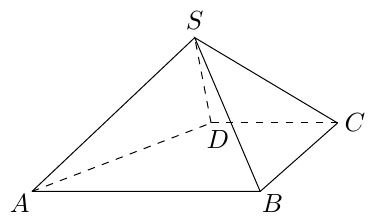
\includegraphics[width=7.4cm]{GaoKao/images/2011/syllabus_science/q19_fig1.png}
\end{center}

        \item 设数列 \(\{a_{n}\}\) 满足 \(a_1 = 0\) 且 \(\frac{1}{1 - a_{n + 1}} -\frac{1}{1 - a_n} = 1\).
\begin{enumerate}
\item 求 \( \{a_{n}\} \) 的通项公式；
\item 设 \( b_n = \frac{1 - \sqrt{a_{n+1}}}{\sqrt{n}} \)，记 \( S_n = \sum_{k=1}^{n} b_k \)，证明：\( S_n < 1 \).
\end{enumerate}

        \item 已知 \(O\) 为坐标原点，\(F\) 为椭圆 \(C: x^2 + \frac{y^2}{2} = 1\) 在 \(y\) 轴正半轴上的焦点，过 \(F\) 且斜率为 \(-\sqrt{2}\) 的直线 \(l\) 与 \(C\) 交于 \(A\)，\(B\) 两点，点 \(P\) 满足 \(\overrightarrow{OA} + \overrightarrow{OB} + \overrightarrow{OP} = 0\).
\begin{enumerate}
\item 证明：点 \(P\) 在 \(C\) 上；
\item 设点 \(P\) 关于点 \(O\) 的对称点为 \(Q\)，证明： \(A\)，\(P\)，\(B\)，\(Q\) 四点在同一圆上.
\end{enumerate}
\begin{center}
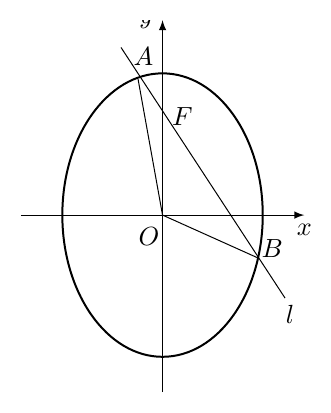
\includegraphics[width=5.5cm]{GaoKao/images/2011/syllabus_science/q21_fig1.png}
\end{center}

    \end{enumerate}

\end{description}

\begin{description}

    \item[四、选考题]

    \begin{enumerate}[leftmargin=5pt]

      \addtocounter{enumi}{+21}

        \item [A]
设函数 \( f(x) = \ln (1 + x) - \frac{2x}{x + 2} \). 证明：当 \( x > 0 \) 时，\( f(x) > 0 \).

        \item [B]
从编号 \(1\) 到 \(100\) 的 \(100\) 张卡片中每次随机抽取一张，然后放回，用这种方式连续抽取 \(20\) 次. 设抽得的 \(20\) 个号码互不相同的概率为 \(p\). 证明：\(p < \left(\frac{9}{10}\right)^{19} < \frac{1}{{\mathrm{e}}^2}\).

    \end{enumerate}

\end{description}


\subsection{2011年大纲卷（文）}\label{gk:2011年大纲卷（文）}

\begin{description}

    \item[一、选择题]

    \begin{enumerate}[leftmargin=5pt]

        \item 设集合 \(U=\{1,2,3,4\}\)，\(M=\{1,2,3\}\)，\(N=\{2,3,4\}\)，则 \(\complement_U(M\cap N)=\)（\quad）

        {\centering\begin{tabular*}{\linewidth}{@{}@{\extracolsep{\fill}}llll@{}}
          \text{A. }\(\{1,2\}\)  &  \text{B. }\(\{2,3\}\)  &  \text{C. }\(\{2,4\}\)  &  \text{D. }\(\{1,4\}\)
        \end{tabular*}\par}

        \item 函数 \(y=2\sqrt{x}\)（\(x\geqslant0\)）的反函数为（\quad）

        {\centering\begin{tabular*}{\linewidth}{@{}@{\extracolsep{\fill}}llll@{}}
          \text{A. }\(y=\frac{x^2}{4}\)（\(x\in\mathbb{R}\)）  &  \text{B. }\(y=\frac{x^2}{4}\)（\(x\geqslant0\)）  &  \text{C. }\(y=4x^2\)（\(x\in\mathbb{R}\)）  &  \text{D. }\(y=4x^2\)（\(x\geqslant0\)）
        \end{tabular*}\par}

        \item 设向量 \(\bm{a}\)，\(\bm{b}\) 满足 \(|\bm{a}|=|\bm{b}|=1\)，\(\bm{a}\cdot\bm{b}=-\frac{1}{2}\)，则 \(|\bm{a}+2\bm{b}|=\)（\quad）

        {\centering\begin{tabular*}{\linewidth}{@{}@{\extracolsep{\fill}}llll@{}}
          \text{A. }\(\sqrt{2}\)  &  \text{B. }\(\sqrt{3}\)  &  \text{C. }\(\sqrt{5}\)  &  \text{D. }\(\sqrt{7}\)
        \end{tabular*}\par}

        \item 若变量 \(x\)，\(y\) 满足约束条件
\(\begin{cases}
x+y\leqslant6,\\
x-3y\leqslant-2,\\
x\geqslant1
\end{cases}\)，则 \(z=2x+3y\) 的最小值为（\quad）

        {\centering\begin{tabular*}{\linewidth}{@{}@{\extracolsep{\fill}}llll@{}}
          \text{A. }\(17\)  &  \text{B. }\(14\)  &  \text{C. }\(5\)  &  \text{D. }\(3\)
        \end{tabular*}\par}

        \item 下面四个条件中，使 \(a>b\) 成立的充分而不必要的条件是（\quad）

        {\centering\begin{tabular*}{\linewidth}{@{}@{\extracolsep{\fill}}llll@{}}
          \text{A. }\(a>b+1\)  &  \text{B. }\(a>b-1\)  &  \text{C. }\(a^2>b^2\)  &  \text{D. }\(a^3>b^3\)
        \end{tabular*}\par}

        \item 设 \(S_n\) 为等差数列 \(\{a_n\}\) 的前 \(n\) 项和. 若 \(a_1=1\)，公差 \(d=2\)，\(S_{k+2}-S_k=24\)，则 \(k=\)（\quad）

        {\centering\begin{tabular*}{\linewidth}{@{}@{\extracolsep{\fill}}llll@{}}
          \text{A. }\(8\)  &  \text{B. }\(7\)  &  \text{C. }\(6\)  &  \text{D. }\(5\)
        \end{tabular*}\par}

        \item 设函数 \(f(x)=\cos\omega x\)（\(\omega>0\)），将 \(y=f(x)\) 的图象向右平移 \(\frac{\pi}{3}\) 个单位长度后，所得的图象与原图象重合，则 \(\omega\) 的最小值等于（\quad）

        {\centering\begin{tabular*}{\linewidth}{@{}@{\extracolsep{\fill}}llll@{}}
          \text{A. }\(\frac{1}{3}\)  &  \text{B. }\(3\)  &  \text{C. }\(6\)  &  \text{D. }\(9\)
        \end{tabular*}\par}

        \item 已知直二面角 \(\alpha-l-\beta\)，点 \(A\in\alpha\)，\(AC\perp l\)，\(C\) 为垂足，点 \(B\in\beta\)，\(BD\perp l\)，\(D\) 为垂足. 若 \(AB=2\)，\(AC=BD=1\)，则 \(CD=\)（\quad）

        {\centering\begin{tabular*}{\linewidth}{@{}@{\extracolsep{\fill}}llll@{}}
          \text{A. }\(2\)  &  \text{B. }\(\sqrt{3}\)  &  \text{C. }\(\sqrt{2}\)  &  \text{D. }\(1\)
        \end{tabular*}\par}

        \item \(4\) 位同学每人从甲，乙，丙 \(3\) 门课程中选修 \(1\) 门，则恰有 \(2\) 人选修课程甲的不同选法共有（\quad）

        {\centering\begin{tabular*}{\linewidth}{@{}@{\extracolsep{\fill}}llll@{}}
          \text{A. }\(12\) 种  &  \text{B. }\(24\) 种  &  \text{C. }\(30\) 种  &  \text{D. }\(36\) 种
        \end{tabular*}\par}

        \item 设 \(f(x)\) 是周期为 \(2\) 的奇函数，当 \(0\leqslant x\leqslant1\) 时，\(f(x)=2x(1-x)\)，则 \(f\left(-\frac{5}{2}\right)=\)（\quad）

        {\centering\begin{tabular*}{\linewidth}{@{}@{\extracolsep{\fill}}llll@{}}
          \text{A. }\(-\frac{1}{2}\)  &  \text{B. }\(-\frac{1}{4}\)  &  \text{C. }\(\frac{1}{4}\)  &  \text{D. }\(\frac{1}{2}\)
        \end{tabular*}\par}

        \item 设两圆 \(C_1\)，\(C_2\) 都和两坐标轴相切，且都过点 \((4,1)\)，则两圆心的距离 \(|C_1C_2|=\)（\quad）

        {\centering\begin{tabular*}{\linewidth}{@{}@{\extracolsep{\fill}}llll@{}}
          \text{A. }\(4\)  &  \text{B. }\(4\sqrt{2}\)  &  \text{C. }\(8\)  &  \text{D. }\(8\sqrt{2}\)
        \end{tabular*}\par}

        \item 已知平面 \(\alpha\) 截一球面得圆 \(M\)，过圆心 \(M\) 且与 \(\alpha\) 成 \(60^{\circ}\) 二面角的平面 \(\beta\) 截该球面得圆 \(N\). 若该球面的半径为 \(4\)，圆 \(M\) 的面积为 \(4\pi\)，则圆 \(N\) 的面积为（\quad）

        {\centering\begin{tabular*}{\linewidth}{@{}@{\extracolsep{\fill}}llll@{}}
          \text{A. }\(7\pi\)  &  \text{B. }\(9\pi\)  &  \text{C. }\(11\pi\)  &  \text{D. }\(13\pi\)
        \end{tabular*}\par}

    \end{enumerate}

\end{description}

\begin{description}

    \item[二、填空题]

    \begin{enumerate}[leftmargin=5pt]

      \addtocounter{enumi}{+12}

        \item \((1-x)^{10}\) 的二项展开式中，\(x\) 的系数与 \(x^9\) 的系数之差为\rule[-0.3ex]{3em}{0.4pt}.

        \item 已知 \(\alpha\in\left(\pi,\frac{3\pi}{2}\right)\)，\(\tan\alpha=2\)，则 \(\cos\alpha=\)\rule[-0.3ex]{3em}{0.4pt}.

        \item 已知正方体 \(ABCD-A_1B_1C_1D_1\) 中，\(E\) 为 \(C_1D_1\) 的中点，则异面直线 \(AE\) 与 \(BC\) 所成角的余弦值为\rule[-0.3ex]{3em}{0.4pt}.

        \item 已知 \(F_1\)，\(F_2\) 分别为双曲线 \(C:\frac{x^2}{9}-\frac{y^2}{27}=1\) 的左，右焦点，点 \(A\in C\)，点 \(M\) 的坐标为 \((2,0)\). \(AM\) 为 \(\angle F_1AF_2\) 的平分线. 则 \(|AF_2|=\)\rule[-0.3ex]{3em}{0.4pt}.

    \end{enumerate}

\end{description}

\begin{description}

    \item[三、解答题]

    \begin{enumerate}[leftmargin=5pt]

      \addtocounter{enumi}{+16}

        \item 设等比数列 \(\{a_n\}\) 的前 \(n\) 项和为 \(S_n\)，已知 \(a_2=6\)，\(6a_1+a_3=30\)，求 \(a_n\) 和 \(S_n\).

        \item \(\triangle ABC\) 的内角 \(A\)，\(B\)，\(C\) 的对边分别为 \(a\)，\(b\)，\(c\). 已知 \(a\sin A+c\sin C-\sqrt{2}a\sin C=b\sin B\).

\begin{enumerate}
\item 求 \(B\)；
\item 若 \(A=75^{\circ}\)，\(b=2\)，求 \(a\)，\(c\).
\end{enumerate}

        \item 根据以往统计资料，某地车主购买甲种保险的概率为 \(0.5\)，购买乙种保险但不购买甲种保险的概率为 \(0.3\). 设各车主购买保险相互独立.

\begin{enumerate}
\item 求该地 \(1\) 位车主至少购买甲，乙两种保险中的 \(1\) 种的概率；
\item 求该地 \(3\) 位车主中恰有 \(1\) 位车主甲，乙两种保险都不购买的概率.
\end{enumerate}

        \item 如图，四棱锥 \(S-ABCD\) 中，\(AB\parallel CD\)，\(BC\perp CD\)，侧面 \(SAB\) 为等边三角形. \(AB=BC=2\)，\(CD=SD=1\).

\begin{enumerate}
\item 证明：\(SD\perp\) 平面 \(SAB\)；
\item 求 \(AB\) 与平面 \(SBC\) 所成角的大小.
\end{enumerate}

\begin{center}
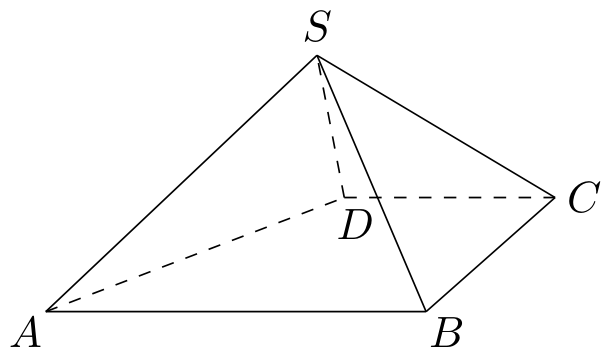
\includegraphics[width=7.1cm]{GaoKao/images/2011/syllabus_liberal/q20_fig1.png}
\end{center}

        \item 已知函数 \(f(x)=x^3+3ax^2+(3-6a)x+12a-4\)（\(a\in\mathbb{R}\)）.

\begin{enumerate}
\item 证明：曲线 \(y=f(x)\) 在 \(x=0\) 处的切线过点 \((2,2)\)；
\item 若 \(f(x)\) 在 \(x=x_0\) 处取得极小值，\(x_0\in(1,3)\)，求 \(a\) 的取值范围.
\end{enumerate}

    \end{enumerate}

\end{description}

\begin{description}

    \item[四、选考题]

    \begin{enumerate}[leftmargin=5pt]

      \addtocounter{enumi}{+21}

        \item \textbf{【选修4-1：几何证明选讲】}

已知 \(O\) 为坐标原点，\(F\) 为椭圆 \(C:x^2+\frac{y^2}{2}=1\) 在 \(y\) 轴正半轴上的焦点，过 \(F\) 且斜率为 \(-\sqrt{2}\) 的直线 \(l\) 与 \(C\) 交于 \(A\)，\(B\) 两点，点 \(P\) 满足 \(\overrightarrow{OA}+\overrightarrow{OB}+\overrightarrow{OP}=0\).

\begin{enumerate}
\item 证明：点 \(P\) 在 \(C\) 上；
\item 设点 \(P\) 关于点 \(O\) 的对称点为 \(Q\)，证明：\(A\)，\(P\)，\(B\)，\(Q\) 四点在同一圆上.
\end{enumerate}

\begin{center}
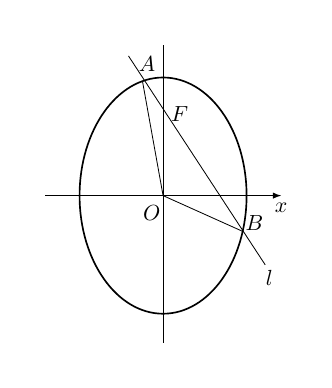
\includegraphics[width=6.0cm]{GaoKao/images/2011/syllabus_liberal/q22_fig1.png}
\end{center}

    \end{enumerate}

\end{description}


\subsection{2011年全国卷（理）}\label{gk:2011年全国卷（理）}

\begin{description}

    \item[一、选择题]

    \begin{enumerate}[leftmargin=5pt]

        \item 复数 \(\frac{2 + \i}{1 - 2\i}\) 的共轭复数是（\quad）

        {\centering\begin{tabular*}{\linewidth}{@{}@{\extracolsep{\fill}}llll@{}}
          \text{A. }\(-\frac{3}{5}\i\)  &  \text{B. }\(\frac{3}{5}\i\)  &  \text{C. }\(-\i\)  &  \text{D. }\(\i\)
        \end{tabular*}\par}

        \item 下列函数中，既是偶函数又在 \(\left(0, +\infty\right)\) 单调递增的函数是（\quad）

        {\centering\begin{tabular*}{\linewidth}{@{}@{\extracolsep{\fill}}llll@{}}
          \text{A. }\(y = x^{3}\)  &  \text{B. }\(y = |x| + 1\)  &  \text{C. }\(y = -x^{2} + 1\)  &  \text{D. }\(y = 2^{-|x|}\)
        \end{tabular*}\par}

        \item 执行如图的程序框图，如果输入的 \(N\) 是 \(6\)，那么输出的 \(p\) 是（\quad）

\begin{center}
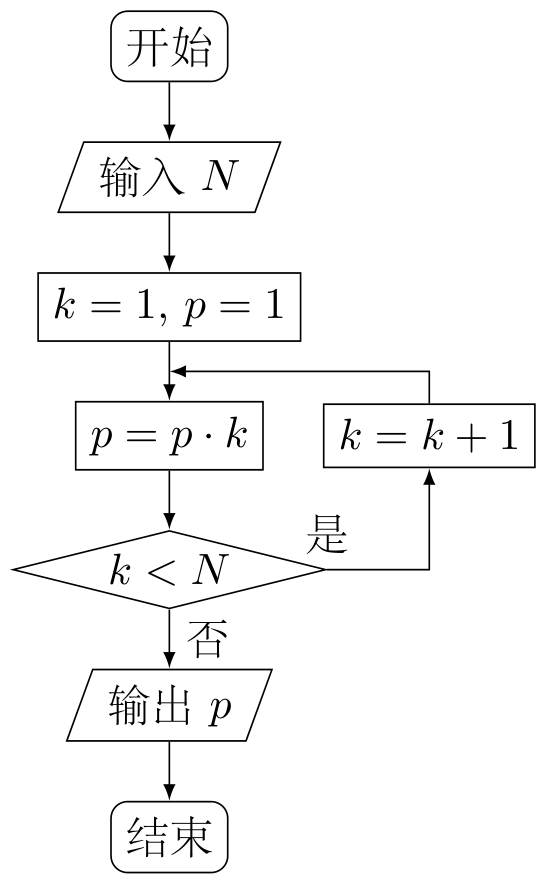
\includegraphics[width=3.2cm]{GaoKao/images/2011/new_curriculum_science/q3_fig1.png}
\end{center}

        {\centering\begin{tabular*}{\linewidth}{@{}@{\extracolsep{\fill}}llll@{}}
          \text{A. }\(120\)  &  \text{B. }\(720\)  &  \text{C. }\(1440\)  &  \text{D. }\(5040\)
        \end{tabular*}\par}

        \item 有 \(3\) 个兴趣小组，甲，乙两位同学各自参加其中一个小组，每位同学参加各个小组的可能性相同，则这两位同学参加同一个兴趣小组的概率为（\quad）

        {\centering\begin{tabular*}{\linewidth}{@{}@{\extracolsep{\fill}}llll@{}}
          \text{A. }\(\frac{1}{3}\)  &  \text{B. }\(\frac{1}{2}\)  &  \text{C. }\(\frac{2}{3}\)  &  \text{D. }\(\frac{3}{4}\)
        \end{tabular*}\par}

        \item 已知角 \(\theta\) 的顶点与原点重合，始边与 \(x\) 轴的正半轴重合，终边在直线 \(y = 2x\) 上，则 \(\cos 2\theta =\)（\quad）

        {\centering\begin{tabular*}{\linewidth}{@{}@{\extracolsep{\fill}}llll@{}}
          \text{A. }\(-\frac{4}{5}\)  &  \text{B. }\(-\frac{3}{5}\)  &  \text{C. }\(\frac{3}{5}\)  &  \text{D. }\(\frac{4}{5}\)
        \end{tabular*}\par}

        \item 在一个几何体的三视图中，正视图和俯视图如下图所示，则相应的侧视图可以为（\quad）

\begin{center}
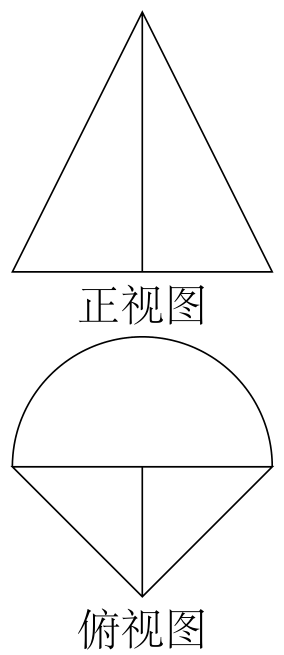
\includegraphics[width=2.8cm]{GaoKao/images/2011/new_curriculum_science/q6_condition.png}
\end{center}

        {\centering\begin{tabular*}{\linewidth}{@{}@{\extracolsep{\fill}}cccc@{}}
          \text{A. }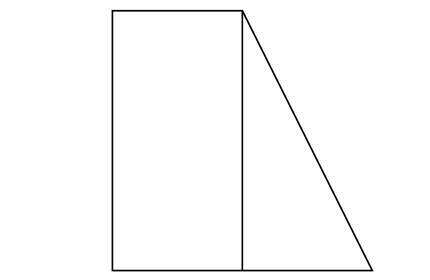
\includegraphics[width=0.15\paperwidth]{GaoKao/images/2011/new_curriculum_science/q6_optA.png}  &  \text{B. }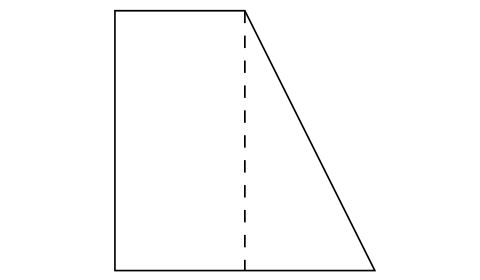
\includegraphics[width=0.15\paperwidth]{GaoKao/images/2011/new_curriculum_science/q6_optB.png}  &  \text{C. }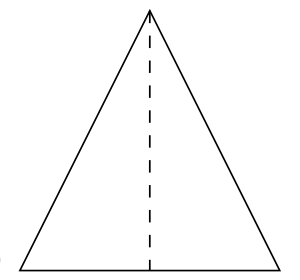
\includegraphics[width=0.15\paperwidth]{GaoKao/images/2011/new_curriculum_science/q6_optC.png}  &  \text{D. }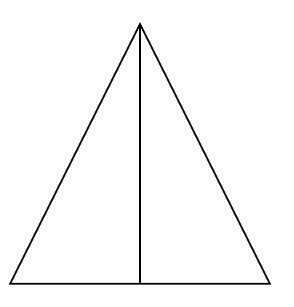
\includegraphics[width=0.15\paperwidth]{GaoKao/images/2011/new_curriculum_science/q6_optD.png}
        \end{tabular*}\par}

        \item 设直线 \(l\) 过双曲线 \(C\) 的一个焦点，且与 \(C\) 的一条对称轴垂直，\(l\) 与 \(C\) 交于 \(A\)，\(B\) 两点，\(|AB|\) 为 \(C\) 的实轴长的 \(2\) 倍，则 \(C\) 的离心率为（\quad）

        {\centering\begin{tabular*}{\linewidth}{@{}@{\extracolsep{\fill}}llll@{}}
          \text{A. }\(\sqrt{2}\)  &  \text{B. }\(\sqrt{3}\)  &  \text{C. }\(2\)  &  \text{D. }\(3\)
        \end{tabular*}\par}

        \item \(\left(x + \frac{a}{x}\right)\left(2x - \frac{1}{x}\right)^5\) 的展开式中各项系数的和为 \(2\)，则该展开式中常数项为（\quad）

        {\centering\begin{tabular*}{\linewidth}{@{}@{\extracolsep{\fill}}llll@{}}
          \text{A. }\(-40\)  &  \text{B. }\(-20\)  &  \text{C. }\(20\)  &  \text{D. }\(40\)
        \end{tabular*}\par}

        \item 由曲线 \(y = \sqrt{x}\)，直线 \(y = x - 2\) 及 \(y\) 轴所围成的图形的面积为（\quad）

        {\centering\begin{tabular*}{\linewidth}{@{}@{\extracolsep{\fill}}llll@{}}
          \text{A. }\(\frac{10}{3}\)  &  \text{B. }\(4\)  &  \text{C. }\( \frac{16}{3} \)  &  \text{D. }\(6\)
        \end{tabular*}\par}

        \item 已知 \(\bm{a}\) 与 \(\bm{b}\) 均为单位向量，其夹角为 \(\theta\)，有下列四个命题：
\begin{enumerate}
    \item \(p_1: |\bm{a} + \bm{b}| > 1 \Leftrightarrow \theta \in \left[0, \frac{2\pi}{3}\right)\)
    \item \(p_2: |\bm{a} + \bm{b}| > 1 \Leftrightarrow \theta \in \left(\frac{2\pi}{3}, \pi\right]\)
    \item \(p_3: |\bm{a} - \bm{b}| > 1 \Leftrightarrow \theta \in \left[0, \frac{\pi}{3}\right)\)
    \item \(p_4: |\bm{a} - \bm{b}| > 1 \Leftrightarrow \theta \in \left(\frac{\pi}{3}, \pi\right]\)
\end{enumerate}
其中的真命题是（\quad）

        {\centering\begin{tabular*}{\linewidth}{@{}@{\extracolsep{\fill}}llll@{}}
          \text{A. }\(p_1\)，\(p_4\)  &  \text{B. }\(p_1\)，\(p_3\)  &  \text{C. }\(p_2\)，\(p_3\)  &  \text{D. }\(p_2\)，\(p_4\)
        \end{tabular*}\par}

        \item 设函数 \( f(x) = \sin\left(\omega x + \varphi\right) + \cos\left(\omega x + \varphi\right) \)（\(\omega > 0\)，\(|\varphi| < \frac{\pi}{2}\)）的最小正周期为 \( \pi \)，且 \( f(-x) = f(x) \)，则（\quad）

        {\centering\begin{tabular*}{\linewidth}{@{}@{\extracolsep{\fill}}llll@{}}
          \text{A. }\(f(x)\) 在 \(\left(0, \frac{\pi}{2}\right)\) 单调递减  &  \text{B. }\(f(x)\) 在 \(\left(\frac{\pi}{4}, \frac{3\pi}{4}\right)\) 单调递减  &  \text{C. }\(f(x)\) 在 \(\left(0, \frac{\pi}{2}\right)\) 单调递增  &  \text{D. }\(f(x)\) 在 \(\left(\frac{\pi}{4}, \frac{3\pi}{4}\right)\) 单调递增
        \end{tabular*}\par}

        \item 函数 \( y = \frac{1}{1 - x} \) 的图象与函数 \( y = 2\sin \pi x \)（\(-2 \leqslant x \leqslant 4\)）的图象所有交点的横坐标之和等于（\quad）

        {\centering\begin{tabular*}{\linewidth}{@{}@{\extracolsep{\fill}}llll@{}}
          \text{A. }\(2\)  &  \text{B. }\(4\)  &  \text{C. }\(6\)  &  \text{D. }\(8\)
        \end{tabular*}\par}

    \end{enumerate}

\end{description}

\begin{description}

    \item[二、填空题]

    \begin{enumerate}[leftmargin=5pt]

      \addtocounter{enumi}{+12}

        \item 若变量 \(x\)，\(y\) 满足约束条件 \(\begin{cases}
3 \leqslant 2x + y \leqslant 9,\\
6 \leqslant x - y \leqslant 9.
\end{cases}\) 则 \(z = x + 2y\) 的最小值为\rule[-0.3ex]{3em}{0.4pt}.

        \item 在平面直角坐标系 \(xOy\) 中，椭圆 \(C\) 的中心为原点，焦点 \(F_{1}\)，\(F_{2}\) 在 \(x\) 轴上，离心率为 \(\frac{\sqrt{2}}{2}\)，过 \(F_{1}\) 的直线 \(l\) 交 \(C\) 于 \(A\)，\(B\) 两点，且 \(\triangle ABF_{2}\) 的周长为 \(16\)，那么 \(C\) 的方程为\rule[-0.3ex]{3em}{0.4pt}.

        \item 已知矩形 \(ABCD\) 的顶点都在半径为 \(4\) 的球 \(O\) 的球面上，且 \(AB = 6\)，\(BC = 2\sqrt{3}\)，则棱锥 \(O - ABCD\) 的体积为\rule[-0.3ex]{3em}{0.4pt}.

        \item 在 \(\triangle ABC\) 中，\(B = 60^{\circ}\)，\(AC = \sqrt{3}\)，则 \(AB + 2BC\) 的最大值为\rule[-0.3ex]{3em}{0.4pt}.

    \end{enumerate}

\end{description}

\begin{description}

    \item[三、解答题]

    \begin{enumerate}[leftmargin=5pt]

      \addtocounter{enumi}{+16}

        \item 等比数列 \(\{a_{n}\}\) 的各项均为正数，且 \(2a_{1} + 3a_{2} = 1\)，\(a_{3}^{2} = 9a_{2}a_{6}\).
\begin{enumerate}
\item 求数列 \( \{a_{n}\} \) 的通项公式；
\item 设 \( b_{n} = \log_{3}a_{1} + \log_{3}a_{2} + \cdots + \log_{3}a_{n} \)，求数列 \( \left\{\frac{1}{b_{n}}\right\} \) 的前 \( n \) 项和.
\end{enumerate}

        \item 如图，四棱锥 \(P - ABCD\) 中，底面 \(ABCD\) 为平行四边形，\(\angle DAB = 60^{\circ}\)，\(AB = 2AD\)，\(PD \perp\) 底面 \(ABCD\).
\begin{enumerate}
\item 证明： \(PA \perp BD\)；
\item 若 \(PD = AD\)，求二面角 \(A - PB - C\) 的余弦值.
\end{enumerate}

\begin{center}
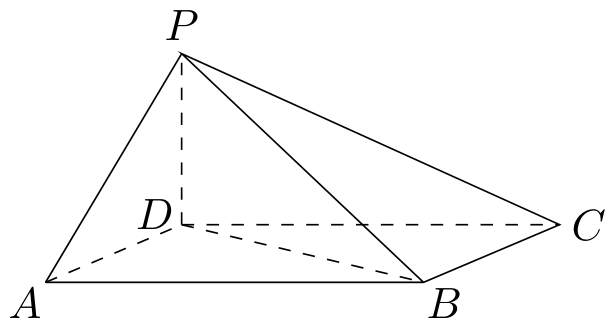
\includegraphics[width=7.6cm]{GaoKao/images/2011/new_curriculum_science/q18_fig1.png}
\end{center}

        \item 某种产品的质量以其质量指标值衡量，质量指标值越大表明质量越好，且质量指标值大于或等于 \(102\) 的产品为优质品. 现用两种新配方（分别称为 A 配方和 B 配方）做试验，各生产了 \(100\) 件这种产品，并测量了每件产品的质量指标值，得到了下面试验结果：

\begin{center}
A 配方的频数分布表

\begin{tabular}{c|c|c|c|c|c}
\hline
指标值分组 & \(\left[90,94\right)\) & \(\left[94,98\right)\) & \(\left[98,102\right)\) & \(\left[102,106\right)\) & \(\left[106,110\right]\) \\
\hline
频数 & \(8\) & \(20\) & \(42\) & \(22\) & \(8\) \\
\hline
\end{tabular}

B 配方的频数分布表

\begin{tabular}{c|c|c|c|c|c}
\hline
指标值分组 & \(\left[90,94\right)\) & \(\left[94,98\right)\) & \(\left[98,102\right)\) & \(\left[102,106\right)\) & \(\left[106,110\right]\) \\
\hline
频数 & \(4\) & \(12\) & \(42\) & \(32\) & \(10\) \\
\hline
\end{tabular}
\end{center}

\begin{enumerate}
\item 分别估计用 A 配方，B 配方生产的产品的优质品率；
\item 已知用 B 配方生产一件产品的利润 \(y\)（单位：元）与其质量指标值 \(t\) 的关系式为 \( y = \begin{cases}
-2, & t < 94,\\
2, & 94 \leqslant t < 102,\\
4, & t \geqslant 102.
\end{cases} \) 从用 B 配方生产的产品中任取一件，其利润记为 \(X\)（单位：元），求 \(X\) 的分布列及数学期望. （以实验结果中质量指标值落入各组的频率作为一件产品的质量指标值落入相应组的概率）.
\end{enumerate}

        \item 在平面直角坐标系 \(xOy\) 中，已知点 \(A\left(0, -1\right)\)，\(B\) 点在直线 \(y = -3\) 上，\(M\) 点满足 \(\overrightarrow{MB} \parallel \overrightarrow{OA}\)，\(\overrightarrow{MA} \cdot \overrightarrow{AB} = \overrightarrow{MB} \cdot \overrightarrow{BA}\)，\(M\) 点的轨迹为曲线 \(C\).
\begin{enumerate}
\item 求 \(C\) 的方程；
\item \(P\) 为 \(C\) 上的动点，\(l\) 为 \(C\) 在 \(P\) 点处的切线，求 \(O\) 点到 \(l\) 距离的最小值.
\end{enumerate}

        \item 已知函数 \( f(x) = a \frac{\ln x}{x + 1} + \frac{b}{x} \)，曲线 \( y = f(x) \) 在点 \(\left(1, f(1)\right)\) 处的切线方程为 \( x + 2y - 3 = 0 \).
\begin{enumerate}
    \item 求 \(a\)，\(b\) 的值；
\item 如果当 \(x > 0\)，且 \(x \neq 1\) 时，\(f(x) > \frac{\ln x}{x - 1} + \frac{k}{x}\)，求 \(k\) 的取值范围.
\end{enumerate}

        \item 如图，\(D\)，\(E\) 分别为 \(\triangle ABC\) 的边 \(AB\)，\(AC\) 上的点，且不与 \(\triangle ABC\) 的顶点重合. 已知 \(AE\) 的长为 \(m\)，\(AC\) 的长为 \(n\)，\(AD\)，\(AB\) 的长是关于 \(x\) 的方程 \(x^{2} - 14x + mn = 0\) 的两个根.
\begin{enumerate}
\item 证明： \(C\)，\(B\)，\(D\)，\(E\) 四点共圆；
\item 若 \(\angle A = 90^{\circ}\)，且 \(m = 4\)，\(n = 6\)，求 \(C\)，\(B\)，\(D\)，\(E\) 所在圆的半径.
\end{enumerate}

\begin{center}
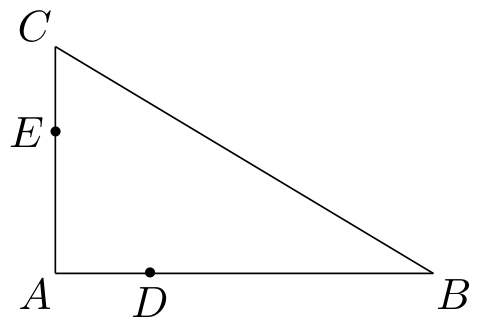
\includegraphics[width=5.9cm]{GaoKao/images/2011/new_curriculum_science/q22_fig1.png}
\end{center}

        \item 在直角坐标系 \(xOy\) 中，曲线 \(C_1\) 的参数方程为 \(\begin{cases}
x = 2\cos \alpha,\\
y = 2 + 2\sin \alpha,
\end{cases}\)（\(\alpha\) 为参数），\(M\) 是 \(C_1\) 上的动点，\(P\) 点满足 \(\overrightarrow{OP} = 2\overrightarrow{OM}\)，\(P\) 点的轨迹为曲线 \(C_2\).
\begin{enumerate}
\item 求 \(C_2\) 的方程；
\item 在以 \(O\) 为极点，\(x\) 轴的正半轴为极轴的极坐标系中，射线 \(\theta = \frac{\pi}{3}\) 与 \(C_1\) 的异于极点的交点为 \(A\)，与 \(C_2\) 的异于极点的交点为 \(B\)，求 \(|AB|\).
\end{enumerate}

        \item 设函数 \(f(x)=|x-a|+3x\)，其中 \(a>0\).
\begin{enumerate}
\item 当 \(a=1\) 时，求不等式 \(f(x)\geqslant 3x+2\) 的解集；
\item 若不等式 \(f(x)\leqslant 0\) 的解集为 \(\{x\mid x\leqslant -1\}\)，求 \(a\) 的值.
\end{enumerate}

    \end{enumerate}

\end{description}


\subsection{2011年全国卷（文）}\label{gk:2011年全国卷（文）}

\begin{description}

    \item[一、选择题]

    \begin{enumerate}[leftmargin=5pt]

        \item 已知集合 \(M = \{0, 1, 2, 3, 4\}\)，\(N = \{1, 3, 5\}\)，\(P = M \cap N\)，则 \(P\) 的子集共有（\quad）

        {\centering\begin{tabular*}{\linewidth}{@{}@{\extracolsep{\fill}}llll@{}}
          \text{A. }\(2\) 个  &  \text{B. }\(4\) 个  &  \text{C. }\(6\) 个  &  \text{D. }\(8\) 个
        \end{tabular*}\par}

        \item 复数 \(\frac{5\i}{1 - 2\i} =\)（\quad）

        {\centering\begin{tabular*}{\linewidth}{@{}@{\extracolsep{\fill}}llll@{}}
          \text{A. }\(2 - \i\)  &  \text{B. }\(1 - 2\i\)  &  \text{C. }\(-2 + \i\)  &  \text{D. }\(-1 + 2\i\)
        \end{tabular*}\par}

        \item 下列函数中，既是偶函数又在 \((0, +\infty)\) 单调递增的函数是（\quad）

        {\centering\begin{tabular*}{\linewidth}{@{}@{\extracolsep{\fill}}llll@{}}
          \text{A. }\(y = x^{3}\)  &  \text{B. }\(y = |x| + 1\)  &  \text{C. }\(y = -x^{2} + 1\)  &  \text{D. }\(y = 2^{-|x|}\)
        \end{tabular*}\par}

        \item 椭圆 \(\frac{x^2}{16} + \frac{y^2}{8} = 1\) 的离心率为（\quad）

        {\centering\begin{tabular*}{\linewidth}{@{}@{\extracolsep{\fill}}llll@{}}
          \text{A. }\( \frac{1}{3} \)  &  \text{B. }\( \frac{1}{2} \)  &  \text{C. }\( \frac{\sqrt{3}}{3} \)  &  \text{D. }\(\frac{\sqrt{2}}{2}\)
        \end{tabular*}\par}

        \item 执行如图的程序框图，如果输入的 \(N\) 是 6，那么输出的 \(p\) 是（\quad）

\begin{center}
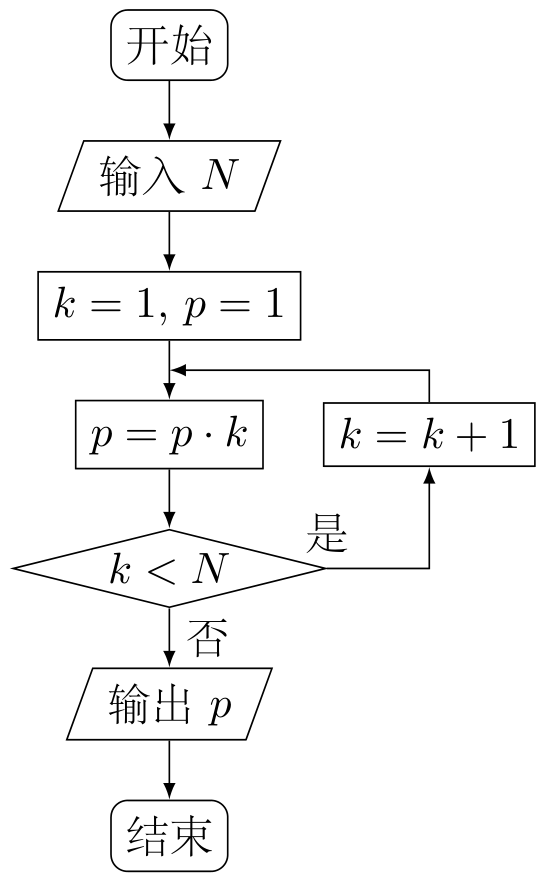
\includegraphics[width=5.1cm]{GaoKao/images/2011/new_curriculum_liberal/q5_flowchart.png}
\end{center}

        {\centering\begin{tabular*}{\linewidth}{@{}@{\extracolsep{\fill}}llll@{}}
          \text{A. }\(120\)  &  \text{B. }\(720\)  &  \text{C. }\(1440\)  &  \text{D. }\(5040\)
        \end{tabular*}\par}

        \item 有 \(3\) 个兴趣小组，甲，乙两位同学各自参加其中一个小组，每位同学参加各个小组的可能性相同，则这两位同学参加同一个兴趣小组的概率为（\quad）

        {\centering\begin{tabular*}{\linewidth}{@{}@{\extracolsep{\fill}}llll@{}}
          \text{A. }\( \frac{1}{3} \)  &  \text{B. }\( \frac{1}{2} \)  &  \text{C. }\( \frac{2}{3} \)  &  \text{D. }\( \frac{3}{4} \)
        \end{tabular*}\par}

        \item 已知角 \(\theta\) 的顶点与原点重合，始边与 \(x\) 轴的正半轴重合，终边在直线 \(y = 2x\) 上，则 \(\cos 2\theta =\)（\quad）

        {\centering\begin{tabular*}{\linewidth}{@{}@{\extracolsep{\fill}}llll@{}}
          \text{A. }\(-\frac{1}{5}\)  &  \text{B. }\(-\frac{3}{5}\)  &  \text{C. }\( \frac{3}{5} \)  &  \text{D. }\( \frac{4}{5} \)
        \end{tabular*}\par}

        \item 在一个几何体的三视图中，正视图和俯视图如下图所示，则相应的侧视图可以为（\quad）

\begin{center}
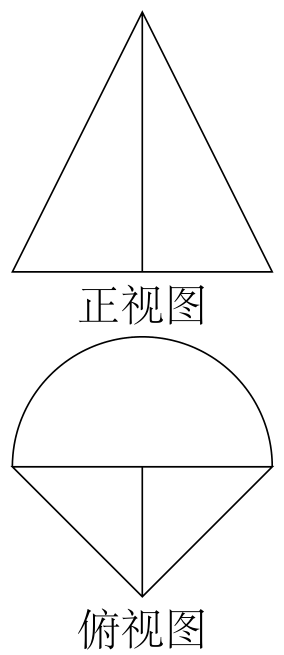
\includegraphics[width=2.8cm]{GaoKao/images/2011/new_curriculum_liberal/q8_condition.png}
\end{center}

        {\centering\begin{tabular*}{\linewidth}{@{}@{\extracolsep{\fill}}cccc@{}}
          \text{A. }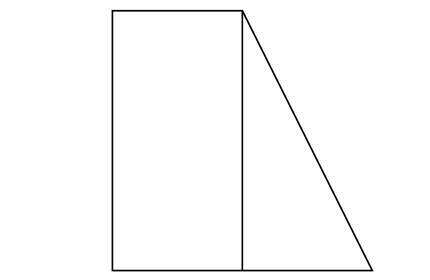
\includegraphics[width=0.15\paperwidth]{GaoKao/images/2011/new_curriculum_liberal/q8_optA.png}  &  \text{B. }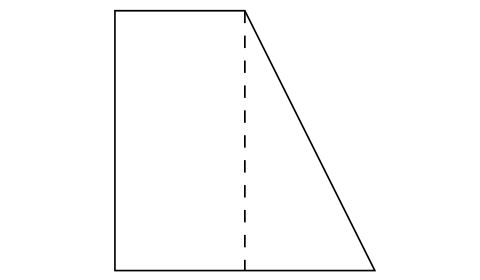
\includegraphics[width=0.15\paperwidth]{GaoKao/images/2011/new_curriculum_liberal/q8_optB.png}  &  \text{C. }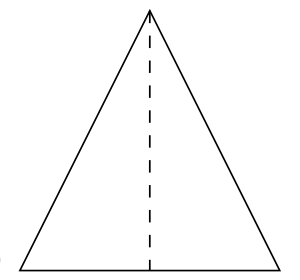
\includegraphics[width=0.15\paperwidth]{GaoKao/images/2011/new_curriculum_liberal/q8_optC.png}  &  \text{D. }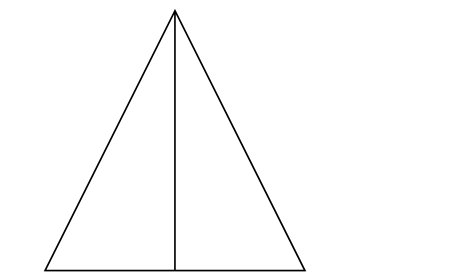
\includegraphics[width=0.15\paperwidth]{GaoKao/images/2011/new_curriculum_liberal/q8_optD.png}
        \end{tabular*}\par}

        \item 已知直线 \(l\) 过抛物线 \(C\) 的焦点，且与 \(C\) 的对称轴垂直，\(l\) 与 \(C\) 交于 \(A, B\) 两点，\( \left|AB\right|=12 \)，\(P\) 为 \(C\) 的准线上一点，则 \( \triangle ABP \) 的面积为（\quad）

        {\centering\begin{tabular*}{\linewidth}{@{}@{\extracolsep{\fill}}llll@{}}
          \text{A. }\(18\)  &  \text{B. }\(24\)  &  \text{C. }\(36\)  &  \text{D. }\(48\)
        \end{tabular*}\par}

        \item 在下列区间中，函数 \( f(x) = {\mathrm{e}}^{x} + 4x - 3 \) 的零点所在的区间为（\quad）

        {\centering\begin{tabular*}{\linewidth}{@{}@{\extracolsep{\fill}}llll@{}}
          \text{A. }\(\left(-\frac{1}{4}, 0\right)\)  &  \text{B. }\(\left(0, \frac{1}{4}\right)\)  &  \text{C. }\(\left(\frac{1}{4}, \frac{1}{2}\right)\)  &  \text{D. }\(\left(\frac{1}{2}, \frac{3}{4}\right)\)
        \end{tabular*}\par}

        \item 设函数 \( f(x) = \sin \left(2x + \frac{\pi}{4}\right) + \cos \left(2x + \frac{\pi}{4}\right) \)，则（\quad）

        {\centering\begin{tabular*}{\linewidth}{@{}@{\extracolsep{\fill}}llll@{}}
          \text{A. }\(y = f(x)\) 在 \(\left(0, \frac{\pi}{2}\right)\) 单调递增，其图象关于直线 \(x = \frac{\pi}{4}\) 对称  &  \text{B. }\(y = f(x)\) 在 \(\left(0, \frac{\pi}{2}\right)\) 单调递增，其图象关于直线 \(x = \frac{\pi}{2}\) 对称  &  \text{C. }\(y = f(x)\) 在 \(\left(0, \frac{\pi}{2}\right)\) 单调递减，其图象关于直线 \(x = \frac{\pi}{4}\) 对称  &  \text{D. }\( y = f(x) \) 在 \( \left(0, \frac{\pi}{2}\right) \) 单调递减，其图象关于直线 \( x = \frac{\pi}{2} \) 对称
        \end{tabular*}\par}

        \item 已知函数 \( y = f(x) \) 的周期为 2，当 \( x \in [-1, 1] \) 时 \( f(x) = x^2 \)，那么函数 \( y = f(x) \) 的图象与函数 \( y = | \lg x | \) 的图象的交点共有（\quad）

        {\centering\begin{tabular*}{\linewidth}{@{}@{\extracolsep{\fill}}llll@{}}
          \text{A. }\(10\) 个  &  \text{B. }\(9\) 个  &  \text{C. }\(8\) 个  &  \text{D. }\(1\) 个
        \end{tabular*}\par}

    \end{enumerate}

\end{description}

\begin{description}

    \item[二、填空题]

    \begin{enumerate}[leftmargin=5pt]

      \addtocounter{enumi}{+12}

        \item 已知 \(\bm{a}\) 与 \(\bm{b}\) 为两个不共线的单位向量，\(k\) 为实数，若向量 \(\bm{a} + \bm{b}\) 与向量 \(k\bm{a} - \bm{b}\) 垂直，则 \(k = \)\rule[-0.3ex]{3em}{0.4pt}.

        \item 若变量 \(x\)，\(y\) 满足约束条件 \(\begin{cases}
3 \leqslant 2x + y \leqslant 9,\\
6 \leqslant x - y \leqslant 9,
\end{cases}\) 则 \(z = x + 2y\) 的最小值为\rule[-0.3ex]{3em}{0.4pt}.

        \item \(\triangle ABC\) 中，\(B = 120^{\circ}\)，\(AC = 7\)，\(AB = 5\)，则 \(\triangle ABC\) 的面积为\rule[-0.3ex]{3em}{0.4pt}.

        \item 已知两个圆锥有公共底面，且两圆锥的顶点和底面的圆周都在同一个球面上. 若圆锥底面面积是这个球面面积的 \(\frac{3}{16}\)，则这两个圆锥中，体积较小者的高与体积较大的高的比值为\rule[-0.3ex]{3em}{0.4pt}.

    \end{enumerate}

\end{description}

\begin{description}

    \item[三、解答题]

    \begin{enumerate}[leftmargin=5pt]

      \addtocounter{enumi}{+16}

        \item 已知等比数列 \(\{a_{n}\}\) 中，\(a_{1} = \frac{1}{3}\)，公比 \(q = \frac{1}{3}\).
\begin{enumerate}
\item 若 \(S_{n}\) 为 \(\{a_{n}\}\) 的前 \(n\) 项和，证明： \(S_{n} = \frac{1 - a_{n}}{2}\)；
\item 设 \(b_{n} = \log_{3} a_{1} + \log_{3} a_{2} + \cdots + \log_{3} a_{n}\)，求数列 \(\{b_{n}\}\) 的通项公式.
\end{enumerate}

        \item 如图，四棱锥 \(P - ABCD\) 中，底面 \(ABCD\) 为平行四边形，\(\angle DAB = 60^{\circ}\)，\(AB = 2AD\)，\(PD \perp\) 底面 \(ABCD\).
\begin{enumerate}
\item 证明： \(PA \perp BD\)；
\item 设 \(PD = AD = 1\)，求棱锥 \(D - PBC\) 的高.
\end{enumerate}

\begin{center}
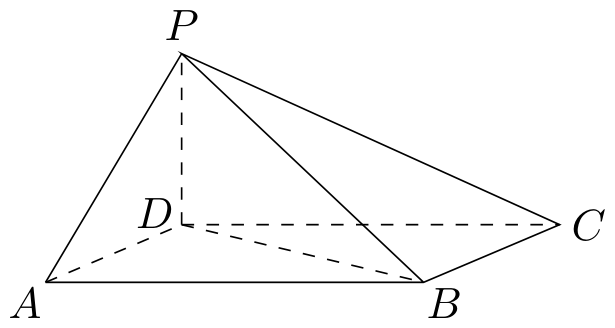
\includegraphics[width=7.6cm]{GaoKao/images/2011/new_curriculum_liberal/q18_pyramid.png}
\end{center}

        \item 某种产品的质量以其质量指标值衡量，质量指标值越大表明质量越好，且质量指标值大于或等于 \(102\) 的产品为优质品. 现用两种新配方（分别称为 A 配方和 B 配方）做试验，各生产了 \(100\) 件这种产品，并测量了每件产品的质量指标值，得到了下面试验结果：

\begin{center}
A 配方的频数分布表

\begin{tabular}{c|ccccc}
\hline
指标值分组 & \(\left[90,94\right)\) & \(\left[94,98\right)\) & \(\left[98,102\right)\) & \(\left[102,106\right)\) & \(\left[106,110\right]\) \\
\hline
频数 & \(8\) & \(20\) & \(42\) & \(22\) & \(8\) \\
\hline
\end{tabular}

B 配方的频数分布表

\begin{tabular}{c|ccccc}
\hline
指标值分组 & \(\left[90,94\right)\) & \(\left[94,98\right)\) & \(\left[98,102\right)\) & \(\left[102,106\right)\) & \(\left[106,110\right]\) \\
\hline
频数 & \(4\) & \(12\) & \(42\) & \(32\) & \(10\) \\
\hline
\end{tabular}
\end{center}

\begin{enumerate}
\item 分别估计用 A 配方，B 配方生产的产品优质品率；
\item 已知用 B 配方生产一件产品的利润 \(y\)（单位：元）与其质量指标值 \(t\) 的关系式为 \(y = \begin{cases}
-2,  t < 94,\\
2,  94 \leqslant t < 102,\\
4,  t \geqslant 102.
\end{cases}\)
估计用 B 配方生产的一件产品的利润大于 \(0\) 的概率，并求用 B 配方生产的上述 \(100\) 件产品平均一件的利润.
\end{enumerate}

        \item 在平面直角坐标系 \(xOy\) 中，曲线 \(y = x^{2} - 6x + 1\) 与坐标轴的交点都在圆 \(C\) 上.
\begin{enumerate}
\item 求圆 \(C\) 的方程；
\item 若圆 \(C\) 与直线 \(x - y + a = 0\) 交于 \(A, B\) 两点，且 \(OA \perp OB\)，求 \(a\) 的值.
\end{enumerate}

        \item 已知函数 \( f(x) = a \frac{\ln x}{x + 1} + \frac{b}{x} \)，曲线 \( y = f(x) \) 在点 \((1, f(1))\) 处的切线方程为 \( x + 2y - 3 = 0 \).
\begin{enumerate}
\item 求 \(a, b\) 的值；
\item 证明：当 \(x > 0\)，且 \(x \neq 1\) 时，\(f(x) > \frac{\ln x}{x - 1}\).
\end{enumerate}

        \item 如图，\(D\)，\(E\) 分别为 \(\triangle ABC\) 的边 \(AB\)，\(AC\) 上的点，且不与 \(\triangle ABC\) 的顶点重合.
已知 \(AE\) 的长为 \(m\)，\(AC\) 的长为 \(n\)，\(AD\)，\(AB\) 的长是关于 \(x\) 的方程 \(x^{2} - 14x + mn = 0\) 的两个根.
\begin{enumerate}
\item 证明： \(C\)，\(B\)，\(D\)，\(E\) 四点共圆；
\item 若 \(\angle A = 90^{\circ}\)，且 \(m = 4\)，\(n = 6\)，求 \(C\)，\(B\)，\(D\)，\(E\) 所在圆的半径.
\end{enumerate}

\begin{center}
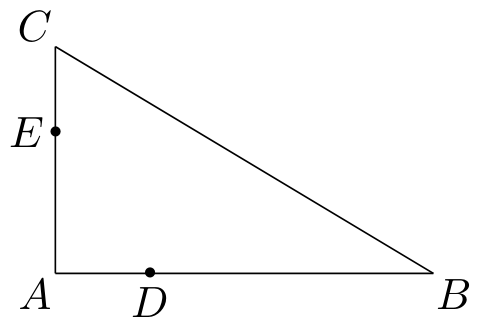
\includegraphics[width=5.9cm]{GaoKao/images/2011/new_curriculum_liberal/q22_triangle.png}
\end{center}

        \item 在直角坐标系 \(xOy\) 中，曲线 \(C_1\) 的参数方程为 \(\begin{cases}
x = 2\cos \alpha,\\
y = 2 + 2\sin \alpha,
\end{cases}\)（\(\alpha\) 为参数），\(M\) 是 \(C_1\) 上的动点，\(P\) 点满足 \(\overrightarrow{OP} = 2\overrightarrow{OM}\)，\(P\) 点的轨迹为曲线 \(C_2\).
\begin{enumerate}
\item 求 \(C_2\) 的方程；
\item 在以 \(O\) 为极点，\(x\) 轴的正半轴为极轴的极坐标系中，射线 \( \theta = \frac{\pi}{3} \) 与 \(C_1\) 的异于极点的交点为 \(A\)，与 \(C_2\) 的异于极点的交点为 \(B\)，求 \(|AB|\).
\end{enumerate}

        \item 设函数 \( f(x) = |x - a| + 3x \)，其中 \( a > 0 \).
\begin{enumerate}
\item 当 \(a = 1\) 时，求不等式 \(f(x) \geqslant 3x + 2\) 的解集；
\item 若不等式 \( f(x) \leqslant 0 \) 的解集为 \( \{x \mid x \leqslant -1\} \)，求 \( a \) 的值.
\end{enumerate}

    \end{enumerate}

\end{description}


\subsection{2011年安徽卷（理）}\label{gk:2011年安徽卷（理）}

\begin{description}

    \item[一、选择题]

    \begin{enumerate}[leftmargin=5pt]

        \item 设 \(\i\) 是虚数单位，复数 \(\frac{1 + a\i}{2 - \i}\) 为纯虚数，则实数 \(a\) 为（\quad）

        {\centering\begin{tabular*}{\linewidth}{@{}@{\extracolsep{\fill}}llll@{}}
          \text{A. }2  &  \text{B. }\(-2\)  &  \text{C. }\(-\frac{1}{2}\)  &  \text{D. }\(\frac{1}{2}\)
        \end{tabular*}\par}

        \item 双曲线 \(2x^{2} - y^{2} = 8\) 的实轴长是（\quad）

        {\centering\begin{tabular*}{\linewidth}{@{}@{\extracolsep{\fill}}llll@{}}
          \text{A. }2  &  \text{B. }\(2\sqrt{2}\)  &  \text{C. }4  &  \text{D. }\(4\sqrt{2}\)
        \end{tabular*}\par}

        \item 设 \( f(x) \) 是定义在 \( \mathbb{R} \) 上的奇函数，当 \( x \leqslant 0 \) 时，\( f(x) = 2x^2 - x \)，则 \( f(1) = \)（\quad）

        {\centering\begin{tabular*}{\linewidth}{@{}@{\extracolsep{\fill}}llll@{}}
          \text{A. }\(-3\)  &  \text{B. }\(-1\)  &  \text{C. }1  &  \text{D. }3
        \end{tabular*}\par}

        \item 设变量 \(x\)，\(y\) 满足 \(|x| + |y| \leqslant 1\)，则 \(x + 2y\) 的最大值和最小值分别为（\quad）

        {\centering\begin{tabular*}{\linewidth}{@{}@{\extracolsep{\fill}}llll@{}}
          \text{A. }1, \(-1\)  &  \text{B. }2, \(-2\)  &  \text{C. }1, \(-2\)  &  \text{D. }2, \(-1\)
        \end{tabular*}\par}

        \item 在极坐标系中，点 \(\left(2, \frac{\pi}{3}\right)\) 到圆 \(\rho = 2\cos \theta\) 的圆心的距离为（\quad）

        {\centering\begin{tabular*}{\linewidth}{@{}@{\extracolsep{\fill}}llll@{}}
          \text{A. }2  &  \text{B. }\(\sqrt{4 + \frac{\pi^2}{9}}\)  &  \text{C. }\(\sqrt{1 + \frac{\pi^2}{9}}\)  &  \text{D. }\(\sqrt{3}\)
        \end{tabular*}\par}

        \item 一个空间几何体的三视图如图所示，则该几何体的表面积为（\quad）

\begin{center}
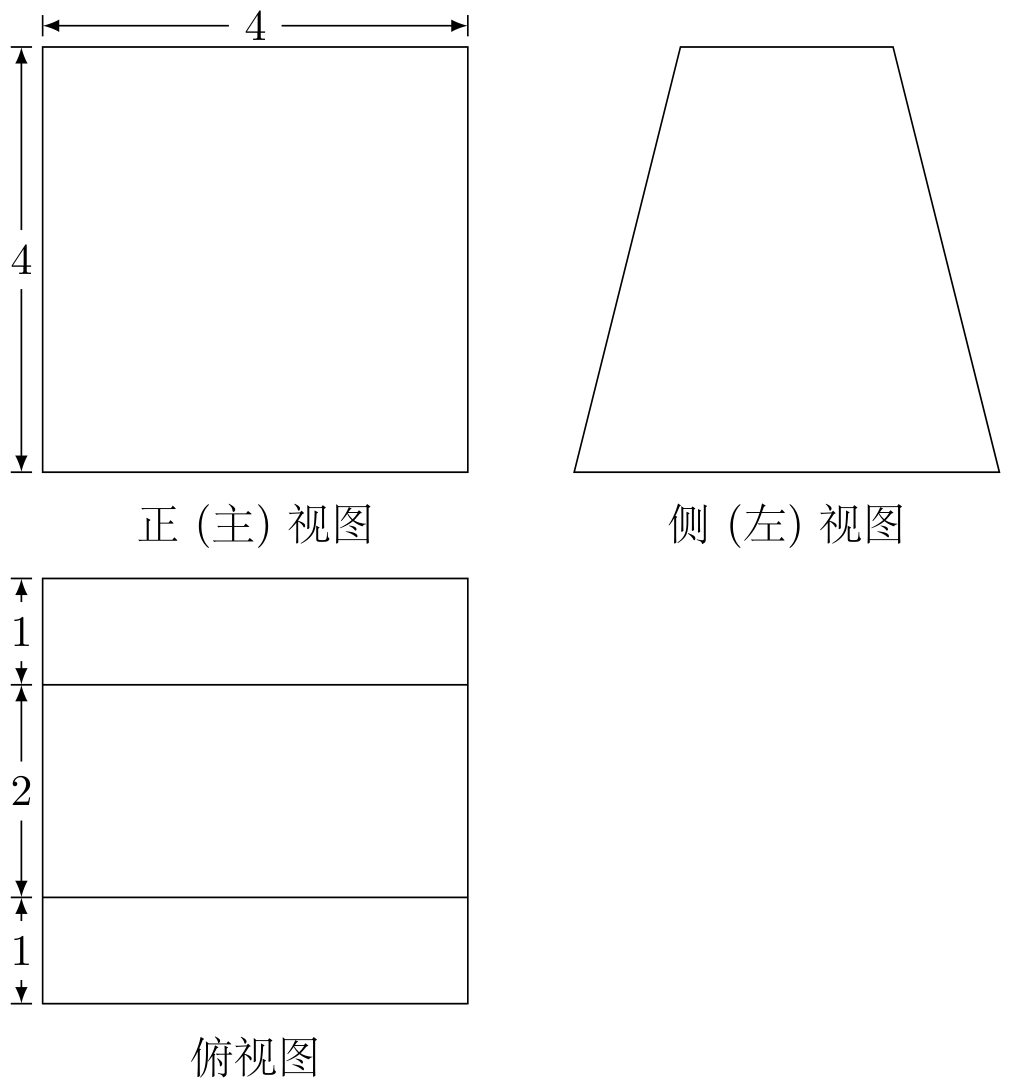
\includegraphics[width=9.9cm]{GaoKao/images/2011/anhui_science/q6_fig1.png}
\end{center}

        {\centering\begin{tabular*}{\linewidth}{@{}@{\extracolsep{\fill}}llll@{}}
          \text{A. }48  &  \text{B. }\(32 + 8\sqrt{17}\)  &  \text{C. }\(48 + 8\sqrt{17}\)  &  \text{D. }80
        \end{tabular*}\par}

        \item 命题“所有能被 2 整除的整数都是偶数”的否定是（\quad）

        {\centering\begin{tabular*}{\linewidth}{@{}@{\extracolsep{\fill}}llll@{}}
          \text{A. }所有不能被 2 整除的整数都是偶数  &  \text{B. }所有能被 2 整除的整数都不是偶数  &  \text{C. }存在一个不能被 2 整除的整数是偶数  &  \text{D. }存在一个能被 2 整除的整数不是偶数
        \end{tabular*}\par}

        \item 设集合 \(A = \{1, 2, 3, 4, 5, 6\}\)，\(B = \{4, 5, 6, 7, 8\}\)，则满足 \(S \subseteq A\) 且 \(S \cap B \neq \varnothing\) 的集合 \(S\) 的个数是（\quad）

        {\centering\begin{tabular*}{\linewidth}{@{}@{\extracolsep{\fill}}llll@{}}
          \text{A. }57  &  \text{B. }56  &  \text{C. }49  &  \text{D. }8
        \end{tabular*}\par}

        \item 已知函数 \( f(x) = \sin (2x + \varphi) \)，其中 \( \varphi \) 为实数，若 \( f(x) \leqslant \left|f\left(\frac{\pi}{6}\right)\right| \) 对 \( x \in \mathbb{R} \) 恒成立，且 \( f\left(\frac{\pi}{2}\right) > f(\pi) \)，则 \( f(x) \) 的单调递增区间是（\quad）

        {\centering\begin{tabular*}{\linewidth}{@{}@{\extracolsep{\fill}}llll@{}}
          \text{A. }\(\left[k\pi - \frac{\pi}{3}, k\pi + \frac{\pi}{6}\right]\)（\(k \in \mathbb{Z}\)）  &  \text{B. }\(\left[k\pi, k\pi + \frac{\pi}{2}\right]\)（\(k \in \mathbb{Z}\)）  &  \text{C. }\(\left[k\pi + \frac{\pi}{6}, k\pi + \frac{2\pi}{3}\right]\)（\(k \in \mathbb{Z}\)）  &  \text{D. }\(\left[k\pi - \frac{\pi}{2}, k\pi\right]\)（\(k \in \mathbb{Z}\)）
        \end{tabular*}\par}

        \item 函数 \( f(x) = ax^{m}(1 - x)^n \) 在区间 \([0,1]\) 上的图象如图所示，则 \(m\)，\(n\) 的值可能是（\quad）

\begin{center}
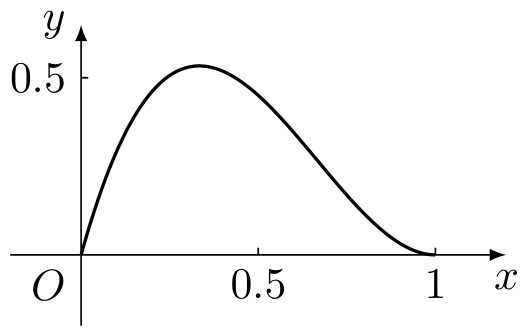
\includegraphics[width=5.0cm]{GaoKao/images/2011/anhui_science/q10_fig1.png}
\end{center}

        {\centering\begin{tabular*}{\linewidth}{@{}@{\extracolsep{\fill}}llll@{}}
          \text{A. }\(m = 1, n = 1\)  &  \text{B. }\(m = 1\)，\(n = 2\)  &  \text{C. }\(m = 2\)，\(n = 1\)  &  \text{D. }\(m = 3\)，\(n = 1\)
        \end{tabular*}\par}

    \end{enumerate}

\end{description}

\begin{description}

    \item[二、填空题]

    \begin{enumerate}[leftmargin=5pt]

      \addtocounter{enumi}{+10}

        \item 如图所示，程序框图（算法流程图）的输出结果是\rule[-0.3ex]{3em}{0.4pt}.

\begin{center}
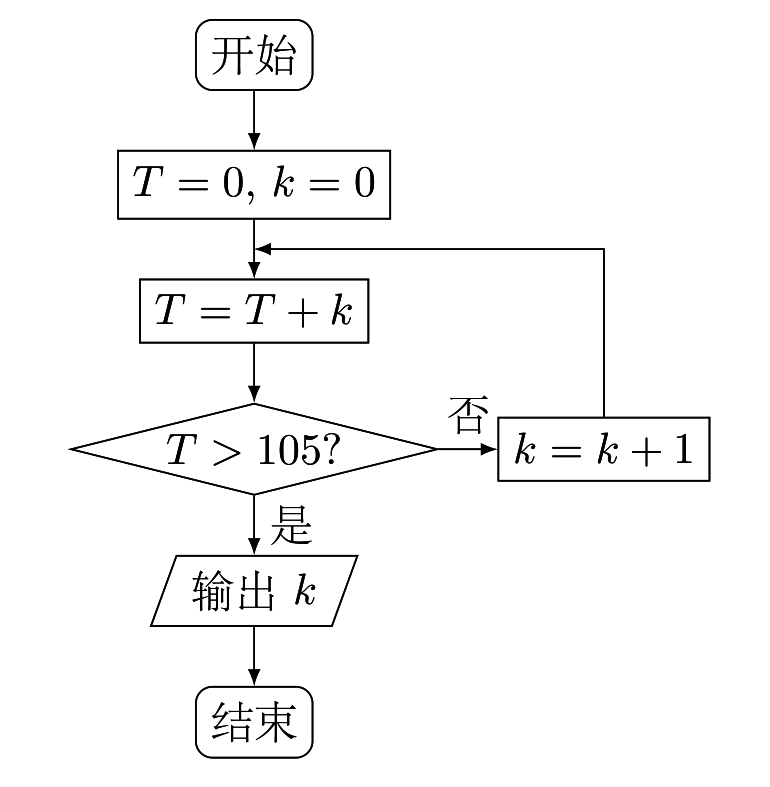
\includegraphics[width=0.42\linewidth]{GaoKao/images/2011/anhui_science/q11_fig1.png}
\end{center}

        \item 设 \((x - 1)^{21} = a_0 + a_1x + a_2x^2 + \dots + a_{21}x^{21}\)，则 \(a_{10} + a_{11} =\rule[-0.3ex]{3em}{0.4pt}\).

        \item 已知向量 \(\bm{a}\)，\(\bm{b}\) 满足 \((\bm{a} + 2\bm{b}) \cdot (\bm{a} - \bm{b}) = -6\)，且 \(|\bm{a}| = 1\)，\(|\bm{b}| = 2\)，则 \(\bm{a}\) 与 \(\bm{b}\) 的夹角为\rule[-0.3ex]{3em}{0.4pt}.

        \item 已知 \(\triangle ABC\) 的一个内角为 \(120^{\circ}\)，并且三边长构成公差为 4 的等差数列，则 \(\triangle ABC\) 的面积为\rule[-0.3ex]{3em}{0.4pt}.

        \item 在平面直角坐标系中，如果 \(x\) 与 \(y\) 都是整数，就称点 \((x, y)\) 为整点，下列命题中正确的是\rule[-0.3ex]{3em}{0.4pt}.（写出所有正确命题的编号）

\begin{enumerate}
\item 存在这样的直线，既不与坐标轴平行又不经过任何整点；
\item 如果 \(k\) 与 \(b\) 都是无理数，则直线 \(y = kx + b\) 不经过任何整点；
\item 直线 \(l\) 经过无穷多个整点，当且仅当 \(l\) 经过两个不同的整点；
\item 直线 \(y = kx + b\) 经过无穷多个整点的充分必要条件是：\(k\) 与 \(b\) 都是有理数；
\item 存在恰经过一个整点的直线.
\end{enumerate}

    \end{enumerate}

\end{description}

\begin{description}

    \item[三、解答题]

    \begin{enumerate}[leftmargin=5pt]

      \addtocounter{enumi}{+15}

        \item 设 \( f(x) = \frac{{\mathrm{e}}^x}{1 + ax^2} \)，其中 \( a \) 为正实数.

\begin{enumerate}
\item 当 \(a=\frac{4}{3}\) 时，求 \( f(x) \) 的极值点；
\item 若 \( f(x) \) 为 \( \mathbb{R} \) 上的单调函数，求 \( a \) 的取值范围.
\end{enumerate}

        \item 如图，\(ABEDFC\) 为多面体，平面 \(ABED\) 与平面 \(ACFD\) 垂直，点 \(O\) 在线段 \(AD\) 上，\(OA = 1\)，\(OD = 2\)，\(\triangle OAB\)，\(\triangle OAC\)，\(\triangle ODE\)，\(\triangle ODF\) 都是正三角形.

\begin{enumerate}
\item 证明直线 \(BC \parallel EF\)；
\item 求棱锥 \(F-OBED\) 的体积.
\end{enumerate}

\begin{center}
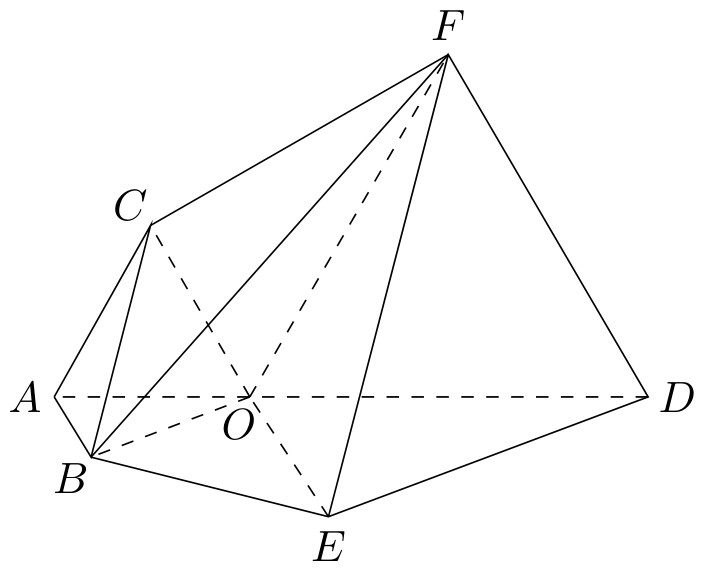
\includegraphics[width=8.2cm]{GaoKao/images/2011/anhui_science/q17_fig1.png}
\end{center}

        \item 在数 1 和 100 之间插入 \(n\) 个实数，使得这 \(n + 2\) 个数构成递增的等比数列，将这 \(n + 2\) 个数的乘积记作 \(T_{n}\)，再令 \(a_{n} = \lg T_{n}\)，\(n \geqslant 1\).

\begin{enumerate}
\item 求数列 \(\{a_{n}\}\) 的通项公式；
\item 设 \(b_{n} = \tan a_{n} \cdot \tan a_{n+1}\)，求数列 \(\{b_{n}\}\) 的前 \(n\) 项和 \(S_{n}\).
\end{enumerate}

        \item \begin{enumerate}
\item 设 \(x \geqslant 1\)，\(y \geqslant 1\)，证明 \(x + y + \frac{1}{xy} \leqslant \frac{1}{x} + \frac{1}{y} + xy\)；
\item \(1 < a \leqslant b \leqslant c\)，证明 \(\log_{a} b + \log_{b} c + \log_{c} a \leqslant \log_{b} a + \log_{c} b + \log_{a} c\).
\end{enumerate}

        \item 工作人员需进入核电站完成某项具有高辐射危险的任务，每次只派一个人进去，且每个人只派一次，工作时间不超过 10 分钟，如果前一个人 10 分钟内不能完成任务则撤出，再派下一个人. 现在一共只有甲，乙，丙三个人可派. 他们各自能完成任务的概率分别 \(p_{1}\)，\(p_{2}\)，\(p_{3}\). 假设 \(p_{1}\)，\(p_{2}\)，\(p_{3}\) 互不相等，且假定各人能否完成任务的事件相互独立.

\begin{enumerate}
\item 如果按甲最先，乙次之，丙最后的顺序派人，求任务能被完成的概率. 若改变三个人被派出的先后顺序，任务能被完成的概率是否发生变化？
\item 若按某指定顺序派人，这三个人各自能完成任务的概率依次为 \(q_{1}\)，\(q_{2}\)，\(q_{3}\)，其中 \(q_{1}\)，\(q_{2}\)，\(q_{3}\) 是 \(p_{1}\)，\(p_{2}\)，\(p_{3}\) 的一个排列. 求所需派出人员数目 \(X\) 的分布列和均值（数学期望）\(E(X)\)；
\item 假定 \(1 > p_{1} > p_{2} > p_{3}\)，试分析以怎样的先后顺序派出人员，可使所需派出的人员数目的均值（数学期望）达到最小.
\end{enumerate}

        \item 设 \(\lambda > 0\)，点 \(A\) 的坐标为 \((1,1)\)，点 \(B\) 在抛物线 \(y = x^2\) 上运动，点 \(Q\) 满足 \(\overrightarrow{BQ} = \lambda \overrightarrow{QA}\)，经过点 \(Q\) 与 \(x\) 轴垂直的直线交抛物线于点 \(M\)，点 \(P\) 满足 \(\overrightarrow{QM} = \lambda \overrightarrow{MP}\)，求点 \(P\) 的轨迹方程.

\begin{center}
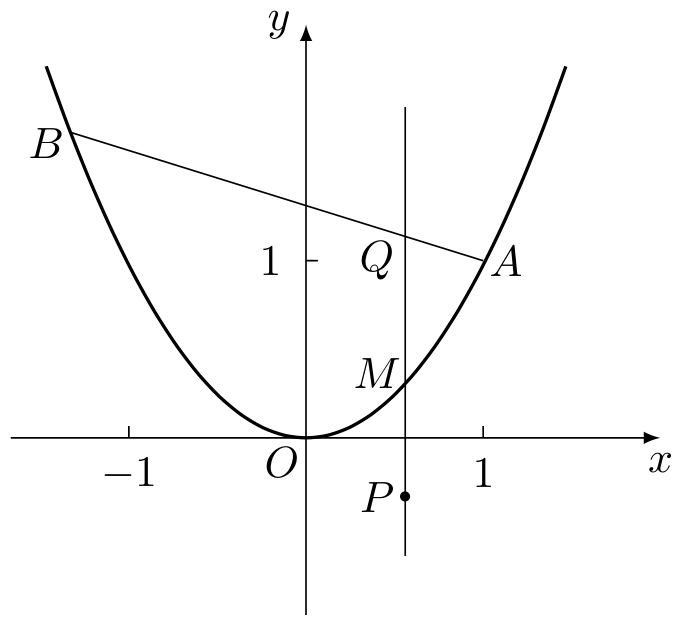
\includegraphics[width=8.5cm]{GaoKao/images/2011/anhui_science/q21_fig1.png}
\end{center}

    \end{enumerate}

\end{description}


\subsection{2011年安徽卷（文）}\label{gk:2011年安徽卷（文）}

\begin{description}

    \item[一、选择题]

    \begin{enumerate}[leftmargin=5pt]

        \item 设 \(\i\) 是虚数单位，复数 \(\frac{1 + a\i}{2 - \i}\) 为纯虚数，则实数 \(a\) 为（\quad）

        {\centering\begin{tabular*}{\linewidth}{@{}@{\extracolsep{\fill}}llll@{}}
          \text{A. }\(2\)  &  \text{B. }\(-2\)  &  \text{C. }\(-\frac{1}{2}\)  &  \text{D. }\(\frac{1}{2}\)
        \end{tabular*}\par}

        \item 集合 \(U = \{1, 2, 3, 4, 5, 6\}\)，\(S = \{1, 4, 5\}\)，\(T = \{2, 3, 4\}\)，则 \(S \cap \left(\complement_{U} T\right)\) 等于（\quad）

        {\centering\begin{tabular*}{\linewidth}{@{}@{\extracolsep{\fill}}llll@{}}
          \text{A. }\(\{1, 4, 5, 6\}\)  &  \text{B. }\(\{1, 5\}\)  &  \text{C. }\(\{4\}\)  &  \text{D. }\(\{1, 2, 3, 4, 5\}\)
        \end{tabular*}\par}

        \item 双曲线 \(2x^{2} - y^{2} = 8\) 的实轴长是（\quad）

        {\centering\begin{tabular*}{\linewidth}{@{}@{\extracolsep{\fill}}llll@{}}
          \text{A. }\(2\)  &  \text{B. }\(2\sqrt{2}\)  &  \text{C. }\(4\)  &  \text{D. }\(4\sqrt{2}\)
        \end{tabular*}\par}

        \item 若直线 \(3x + y + a = 0\) 过圆 \(x^{2} + y^{2} + 2x - 4y = 0\) 的圆心，则 \(a\) 的值为（\quad）

        {\centering\begin{tabular*}{\linewidth}{@{}@{\extracolsep{\fill}}llll@{}}
          \text{A. }\(-1\)  &  \text{B. }\(1\)  &  \text{C. }\(3\)  &  \text{D. }\(-3\)
        \end{tabular*}\par}

        \item 若点 \((a, b)\) 在 \(y = \lg x\) 图象上，\(a \neq 1\)，则下列点中在此图象上的是（\quad）

        {\centering\begin{tabular*}{\linewidth}{@{}@{\extracolsep{\fill}}llll@{}}
          \text{A. }\(\left(\frac{1}{a}, b\right)\)  &  \text{B. }\((10a, 1 - b)\)  &  \text{C. }\(\left(\frac{10}{a}, b + 1\right)\)  &  \text{D. }\((a^{2}, 2b)\)
        \end{tabular*}\par}

        \item 设变量 \(x\)，\(y\) 满足 \(\begin{cases}
x + y \leqslant 1,\\
x - y \leqslant 1,\\
x \geqslant 0,
\end{cases}\)
则 \(x + 2y\) 的最大值和最小值分别为（\quad）

        {\centering\begin{tabular*}{\linewidth}{@{}@{\extracolsep{\fill}}llll@{}}
          \text{A. }\(1\)，\(-1\)  &  \text{B. }\(2\)，\(-2\)  &  \text{C. }\(1\)，\(-2\)  &  \text{D. }\(2\)，\(-1\)
        \end{tabular*}\par}

        \item 若数列 \(\{a_{n}\}\) 的通项公式是 \(a_{n} = (-1)^{n}(3n - 2)\)，则 \(a_{1} + a_{2} + \cdots + a_{10} =\)（\quad）

        {\centering\begin{tabular*}{\linewidth}{@{}@{\extracolsep{\fill}}llll@{}}
          \text{A. }\(15\)  &  \text{B. }\(12\)  &  \text{C. }\(-12\)  &  \text{D. }\(-15\)
        \end{tabular*}\par}

        \item 一个空间几何体的三视图如图所示，则该几何体的表面积为（\quad）

\begin{center}
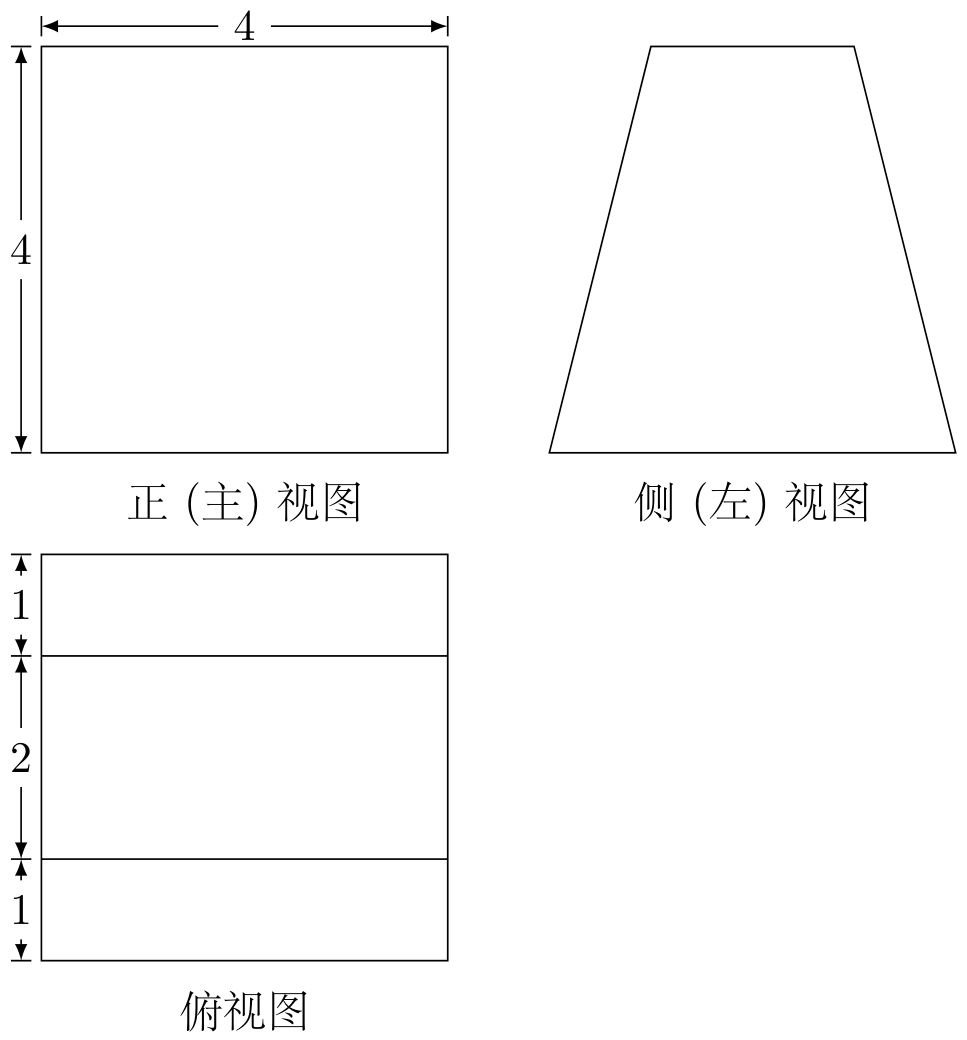
\includegraphics[width=9.5cm]{GaoKao/images/2011/anhui_liberal/q8_fig1.png}
\end{center}

        {\centering\begin{tabular*}{\linewidth}{@{}@{\extracolsep{\fill}}llll@{}}
          \text{A. }\(48\)  &  \text{B. }\(32 + 8\sqrt{17}\)  &  \text{C. }\(48 + 8\sqrt{17}\)  &  \text{D. }\(80\)
        \end{tabular*}\par}

        \item 从正六边形的 6 个顶点中随机选择 4 个顶点，则以它们作为顶点的四边形是矩形的概率等于（\quad）

        {\centering\begin{tabular*}{\linewidth}{@{}@{\extracolsep{\fill}}llll@{}}
          \text{A. }\(\frac{1}{10}\)  &  \text{B. }\(\frac{1}{8}\)  &  \text{C. }\(\frac{1}{6}\)  &  \text{D. }\(\frac{1}{5}\)
        \end{tabular*}\par}

        \item 函数 \(f(x) = ax^{n}(1 - x)^{2}\) 在区间 \([0, 1]\) 上的图象如图所示，则 \(n\) 可能是（\quad）

\begin{center}
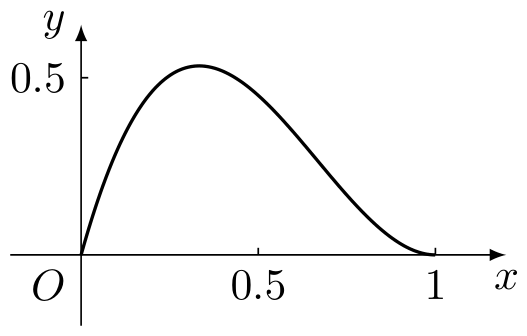
\includegraphics[width=5.0cm]{GaoKao/images/2011/anhui_liberal/q10_fig1.png}
\end{center}

        {\centering\begin{tabular*}{\linewidth}{@{}@{\extracolsep{\fill}}llll@{}}
          \text{A. }\(1\)  &  \text{B. }\(2\)  &  \text{C. }\(3\)  &  \text{D. }\(4\)
        \end{tabular*}\par}

    \end{enumerate}

\end{description}

\begin{description}

    \item[二、填空题]

    \begin{enumerate}[leftmargin=5pt]

      \addtocounter{enumi}{+10}

        \item 设 \(f(x)\) 是定义在 \(\mathbb{R}\) 上的奇函数，当 \(x \leqslant 0\) 时，\(f(x) = 2x^{2} - x\)，则 \(f(1) =\rule[-0.3ex]{3em}{0.4pt}\).

        \item 如图所示，程序框图（算法流程图）的输出结果是\rule[-0.3ex]{3em}{0.4pt}.

\begin{center}
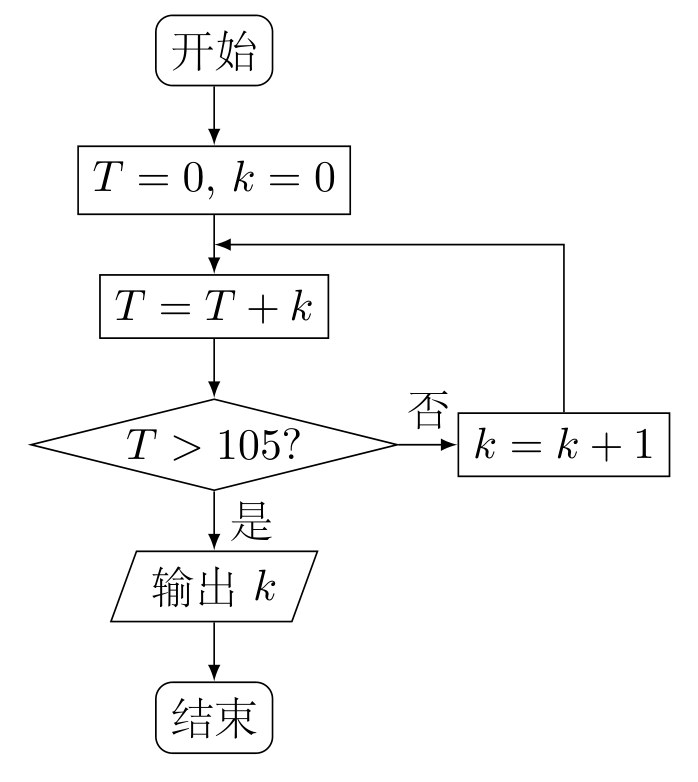
\includegraphics[width=0.5\linewidth]{GaoKao/images/2011/anhui_liberal/q12_fig1.png}
\end{center}

        \item 函数 \(y = \frac{1}{\sqrt{6 - x - x^{2}}}\) 的定义域是\rule[-0.3ex]{3em}{0.4pt}.

        \item 已知向量 \(\bm{a}\)，\(\bm{b}\) 满足 \((\bm{a} + 2\bm{b}) \cdot (\bm{a} - \bm{b}) = -6\)，且 \(|\bm{a}| = 1\)，\(|\bm{b}| = 2\)，则 \(\bm{a}\) 与 \(\bm{b}\) 的夹角为\rule[-0.3ex]{3em}{0.4pt}.

        \item 设 \(f(x) = a\sin 2x + b\cos 2x\)，其中 \(a\)，\(b \in \mathbb{R}\)，\(ab \neq 0\)，若 \(f(x) \leqslant \left|f\left(\frac{\pi}{6}\right)\right|\) 对一切 \(x \in \mathbb{R}\) 恒成立，则
\begin{enumerate}
\item \(f\left(\frac{11\pi}{12}\right) = 0\)；
\item \(f\left(\frac{7\pi}{10}\right) < \left|f\left(\frac{\pi}{5}\right)\right|\)；
\item \(f(x)\) 既不是奇函数，也不是偶函数；
\item \(f(x)\) 的单调递增区间是 \(\left[k\pi + \frac{\pi}{6}, k\pi + \frac{2\pi}{3}\right]\)（\(k \in \mathbb{Z}\)）；
\item 存在经过点 \((a, b)\) 的直线与函数 \(f(x)\) 的图象不相交.
\end{enumerate}
以上结论正确的是\rule[-0.3ex]{3em}{0.4pt}.（写出所有正确结论的编号）

    \end{enumerate}

\end{description}

\begin{description}

    \item[三、解答题]

    \begin{enumerate}[leftmargin=5pt]

      \addtocounter{enumi}{+15}

        \item 在 \(\triangle ABC\) 中，\(a\)，\(b\)，\(c\) 分别为内角 \(A\)，\(B\)，\(C\) 所对的边长，\(a = \sqrt{3}\)，\(b = \sqrt{2}\)，\(1 + 2\cos(B + C) = 0\)，求边 \(BC\) 上的高.

        \item 设直线 \(l_{1} : y = k_{1}x + 1\)，\(l_{2} : y = k_{2}x - 1\)，其中实数 \(k_{1}\)，\(k_{2}\) 满足 \(k_{1}k_{2} + 2 = 0\).
\begin{enumerate}
\item 证明 \(l_{1}\) 与 \(l_{2}\) 相交；
\item 证明 \(l_{1}\) 与 \(l_{2}\) 的交点在椭圆 \(2x^{2} + y^{2} = 1\) 上.
\end{enumerate}

        \item 设 \(f(x) = \frac{{\mathrm{e}}^{x}}{1 + ax^{2}}\)，其中 \(a\) 为正实数.
\begin{enumerate}
\item 当 \(a = \frac{4}{3}\) 时，求 \(f(x)\) 的极值点；
\item 若 \(f(x)\) 为 \(\mathbb{R}\) 上的单调函数，求 \(a\) 的取值范围.
\end{enumerate}

        \item 如图，\(ABEDFC\) 为多面体，平面 \(ABED\) 与平面 \(ACFD\) 垂直，点 \(O\) 在线段 \(AD\) 上，\(OA = 1\)，\(OD = 2\)，\(\triangle OAB\)，\(\triangle OAC\)，\(\triangle ODE\)，\(\triangle ODF\) 都是正三角形.

\begin{enumerate}
\item 证明直线 \(BC \parallel EF\)；
\item 求棱锥 \(F - OBED\) 的体积.
\end{enumerate}

\begin{center}
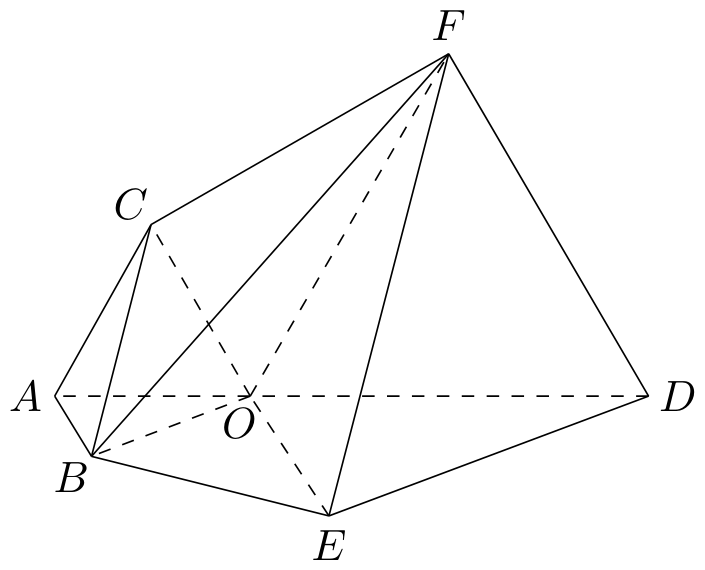
\includegraphics[width=8.8cm]{GaoKao/images/2011/anhui_liberal/q19_fig1.png}
\end{center}

        \item 某地最近十年粮食需求量逐年上升，下表是部分统计数据：

\begin{center}
\begin{tabular}{c|ccccc}
年份 & \(2002\) & \(2004\) & \(2006\) & \(2008\) & \(2010\) \\
\hline
需求量（\(\text{万吨}\)） & \(236\) & \(246\) & \(257\) & \(276\) & \(286\)
\end{tabular}
\end{center}

\begin{enumerate}
\item 利用所给数据求年需求量与年份之间的回归直线方程 \(\hat{y} = bx + a\)；
\item 利用（1）中所求出的直线方程预测该地 \(2012\) 年的粮食需求量.
\end{enumerate}

        \item 在数 \(1\) 和 \(100\) 之间插入 \(n\) 个实数，使得这 \(n + 2\) 个数构成递增的等比数列，将这 \(n + 2\) 个数的乘积记作 \(T_{n}\)，再令 \(a_{n} = \lg T_{n}\)，\(n \geqslant 1\).
\begin{enumerate}
\item 求数列 \(\{a_{n}\}\) 的通项公式；
\item 设 \(b_{n} = \tan a_{n} \cdot \tan a_{n+1}\)，求数列 \(\{b_{n}\}\) 的前 \(n\) 项和 \(S_{n}\).
\end{enumerate}

    \end{enumerate}

\end{description}


\subsection{2011年北京卷（理）}\label{gk:2011年北京卷（理）}

\begin{description}

    \item[一、选择题]

    \begin{enumerate}[leftmargin=5pt]

        \item 已知集合 \(P = \{x \mid x^2 \leqslant 1\}\)，\(M = \{a\}\). 若 \(P \cup M = P\)，则 \(a\) 的取值范围是（\quad）

        {\centering\begin{tabular*}{\linewidth}{@{}@{\extracolsep{\fill}}llll@{}}
          \text{A. }\((- \infty, -1]\)  &  \text{B. }\([1, +\infty)\)  &  \text{C. }\([-1, 1]\)  &  \text{D. }\((- \infty, -1] \cup [1, +\infty)\)
        \end{tabular*}\par}

        \item 复数 \(\frac{\i-2}{1+2\i}=\)（\quad）

        {\centering\begin{tabular*}{\linewidth}{@{}@{\extracolsep{\fill}}llll@{}}
          \text{A. }\(\i\)  &  \text{B. }\(-\i\)  &  \text{C. }\(-\frac{4}{5} - \frac{3}{5}\i\)  &  \text{D. }\(-\frac{4}{5} + \frac{3}{5}\i\)
        \end{tabular*}\par}

        \item 在极坐标系中，圆 \(\rho = -2\sin \theta\) 的圆心的极坐标是（\quad）

        {\centering\begin{tabular*}{\linewidth}{@{}@{\extracolsep{\fill}}llll@{}}
          \text{A. }\(\left(1, \frac{\pi}{2}\right)\)  &  \text{B. }\(\left(1, -\frac{\pi}{2}\right)\)  &  \text{C. }\((1, 0)\)  &  \text{D. }\((1, \pi)\)
        \end{tabular*}\par}

        \item 执行如图所示的程序框图，输出的 \(s\) 的值为（\quad）

\begin{center}
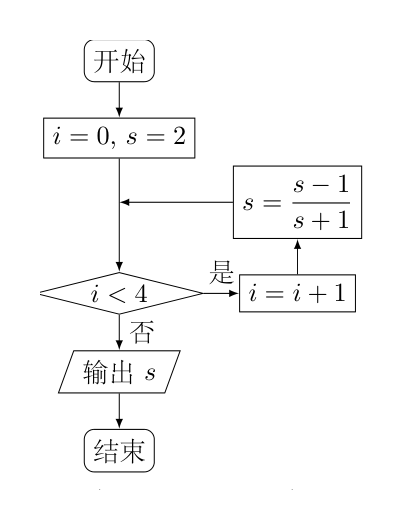
\includegraphics[width=0.65\linewidth]{GaoKao/images/2011/beijing_science/q4_fig1.png}
\end{center}

        {\centering\begin{tabular*}{\linewidth}{@{}@{\extracolsep{\fill}}llll@{}}
          \text{A. }\(-3\)  &  \text{B. }\(\frac{1}{2}\)  &  \text{C. }\(\frac{1}{3}\)  &  \text{D. }\(2\)
        \end{tabular*}\par}

        \item 如图，\(AD\)，\(AE\)，\(BC\) 分别与圆 \(O\) 切于点 \(D\)，\(E\)，\(F\)，延长 \(AF\) 与圆 \(O\) 交于另一点 \(G\). 给出下列三个结论：

\begin{enumerate}
\item \(AD + AE = AB + BC + CA\)；
\item \(AF \cdot AG = AD \cdot AE\)；
\item \(\triangle AFB \sim \triangle ADG\).
\end{enumerate}

其中正确结论的序号是（\quad）

\begin{center}
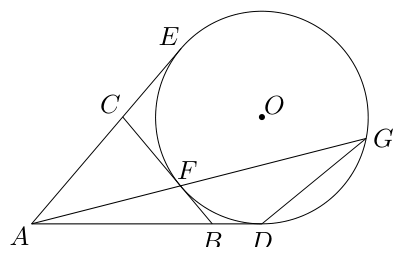
\includegraphics[width=10.0cm]{GaoKao/images/2011/beijing_science/q5_fig1.png}
\end{center}

        {\centering\begin{tabular*}{\linewidth}{@{}@{\extracolsep{\fill}}llll@{}}
          \text{A. }\(\ding{172}\ding{173}\)  &  \text{B. }\(\ding{173}\ding{174}\)  &  \text{C. }\(\ding{172}\ding{174}\)  &  \text{D. }\(\ding{172}\ding{173}\ding{174}\)
        \end{tabular*}\par}

        \item 根据统计，一名工人组装第 \(x\) 件某产品所用的时间（单位：分钟）为
\(f(x) = \begin{cases}
\dfrac{c}{\sqrt{x}}, & x < A,\\
\dfrac{c}{\sqrt{A}}, & x \geqslant A,
\end{cases}\)
（\(A\)，\(c\) 为常数）. 已知工人组装第 \(4\) 件产品用时 \(30\) 分钟，组装第 \(A\) 件产品用时 \(15\) 分钟，那么 \(c\) 和 \(A\) 的值分别是（\quad）

        {\centering\begin{tabular*}{\linewidth}{@{}@{\extracolsep{\fill}}llll@{}}
          \text{A. }\((75, 25)\)  &  \text{B. }\((75, 16)\)  &  \text{C. }\((60, 25)\)  &  \text{D. }\((60, 16)\)
        \end{tabular*}\par}

        \item 某四面体的三视图如图所示，该四面体四个面的面积中最大的是（\quad）

\begin{center}
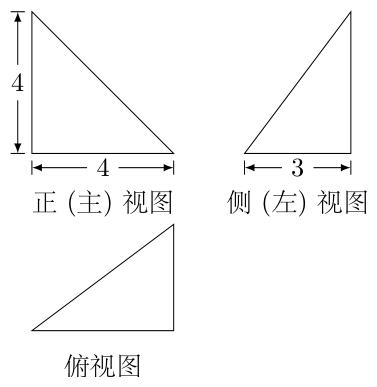
\includegraphics[width=6.2cm]{GaoKao/images/2011/beijing_science/q7_fig1.png}
\end{center}

        {\centering\begin{tabular*}{\linewidth}{@{}@{\extracolsep{\fill}}llll@{}}
          \text{A. }\(8\)  &  \text{B. }\(6\sqrt{2}\)  &  \text{C. }\(10\)  &  \text{D. }\(8\sqrt{2}\)
        \end{tabular*}\par}

        \item 设 \(A(0, 0)\)，\(B(4, 0)\)，\(C(t + 4, 4)\)，\(D(t, 4)\)（\(t \in \mathbb{R}\)）. 记 \(N(t)\) 为平行四边形 \(ABCD\) 内部（不含边界）的整点的个数，其中整点是指横，纵坐标都是整数的点，则函数 \(N(t)\) 的值域为（\quad）

        {\centering\begin{tabular*}{\linewidth}{@{}@{\extracolsep{\fill}}llll@{}}
          \text{A. }\(\{9, 10, 11\}\)  &  \text{B. }\(\{9, 10, 12\}\)  &  \text{C. }\(\{9, 11, 12\}\)  &  \text{D. }\(\{10, 11, 12\}\)
        \end{tabular*}\par}

    \end{enumerate}

\end{description}

\begin{description}

    \item[二、填空题]

    \begin{enumerate}[leftmargin=5pt]

      \addtocounter{enumi}{+8}

        \item 在 \(\triangle ABC\) 中，若 \(b = 5\)，\(\angle B = \frac{\pi}{4}\)，\(\tan A = 2\)，则 \(\sin A=\)\rule[-0.3ex]{3em}{0.4pt}；\(a=\)\rule[-0.3ex]{3em}{0.4pt}.

        \item 已知向量 \(\bm{a} = (\sqrt{3}, 1)\)，\(\bm{b} = (0, -1)\)，\(\bm{c} = (k, \sqrt{3})\). 若 \(\bm{a} - 2\bm{b}\) 与 \(\bm{c}\) 共线，则 \(k=\)\rule[-0.3ex]{3em}{0.4pt}.

        \item 在等比数列 \(\{a_n\}\) 中，\(a_1 = \frac{1}{2}\)，\(a_4 = -4\)，则公比 \(q=\)\rule[-0.3ex]{3em}{0.4pt}；\(|a_1| + |a_2| + \cdots + |a_n| = \)\rule[-0.3ex]{3em}{0.4pt}.

        \item 用数字 \(2\)，\(3\) 组成四位数，且数字 \(2\)，\(3\) 至少都出现一次，这样的四位数共有\rule[-0.3ex]{3em}{0.4pt} 个（用数字作答）.

        \item 已知函数 \(f(x) = \begin{cases}
\dfrac{2}{x}, & x \geqslant 2,\\
(x - 1)^3, & x < 2,
\end{cases}\)
若关于 \(x\) 的方程 \(f(x) = k\) 有两个不同的实根，则实数 \(k\) 的取值范围是\rule[-0.3ex]{3em}{0.4pt}.

        \item 曲线 \(C\) 是平面内与两个定点 \(F_1(-1, 0)\) 和 \(F_2(1, 0)\) 的距离的积等于常数 \(a^2\)（\(a > 1\)）的点的轨迹. 给出下列三个结论：

\begin{enumerate}
\item 曲线 \(C\) 过坐标原点；
\item 曲线 \(C\) 关于坐标原点对称；
\item 若点 \(P\) 在曲线 \(C\) 上，则 \(\triangle F_1PF_2\) 的面积不大于 \(\frac{1}{2}a^2\).
\end{enumerate}

其中所有正确结论的序号是\rule[-0.3ex]{3em}{0.4pt}.

    \end{enumerate}

\end{description}

\begin{description}

    \item[三、解答题]

    \begin{enumerate}[leftmargin=5pt]

      \addtocounter{enumi}{+14}

        \item 已知函数 \(f(x) = 4\cos x\sin \left(x + \frac{\pi}{6}\right) - 1\).

\begin{enumerate}
\item 求 \(f(x)\) 的最小正周期；
\item 求 \(f(x)\) 在区间 \(\left[-\frac{\pi}{6}, \frac{\pi}{4}\right]\) 上的最大值和最小值.
\end{enumerate}

        \item 如图，在四棱锥 \(P - ABCD\) 中，\(PA \perp\) 平面 \(ABCD\)，底面 \(ABCD\) 是菱形，\(AB = 2\)，\(\angle BAD = 60^{\circ}\).

\begin{enumerate}
\item 求证：\(BD \perp\) 平面 \(PAC\)；
\item 若 \(PA = AB\)，求 \(PB\) 与 \(AC\) 所成角的余弦值；
\item 当平面 \(PBC\) 与平面 \(PDC\) 垂直时，求 \(PA\) 的长.
\end{enumerate}

\begin{center}
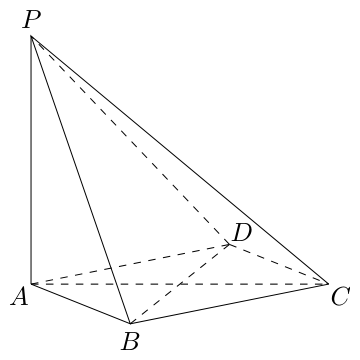
\includegraphics[width=9.7cm]{GaoKao/images/2011/beijing_science/q16_fig1.png}
\end{center}

        \item 以下茎叶图记录了甲，乙两组各四名同学的植树棵数. 乙组记录中有一个数据模糊，无法确认，在图中以 \(X\) 表示.

\begin{center}
\begin{tabular}{c|c|c}
甲组 & 茎 & 乙组 \\
\hline
\(9\quad 9\) & \(0\) & \(X\quad 8\quad 9\) \\
\(1\quad 1\) & \(1\) & \(0\)
\end{tabular}
\end{center}

\begin{enumerate}
\item 如果 \(X = 8\)，求乙组同学植树棵数的平均数和方差；
\item 如果 \(X = 9\)，分别从甲，乙两组中随机选取一名同学，求这两名同学的植树总棵数 \(Y\) 的分布列和数学期望.
\end{enumerate}

（注：方差 \(s^2 = \frac{1}{n}\left[(x_1 - \bar{x})^2 + (x_2 - \bar{x})^2 + \cdots + (x_n - \bar{x})^2\right]\)，其中 \(\bar{x}\) 为 \(x_1\)，\(x_2\)，\(\cdots\)，\(x_n\) 的平均数）

        \item 已知函数 \(f(x) = (x - k)^2{\mathrm{e}}^{\frac{x}{k}}\).

\begin{enumerate}
\item 求 \(f(x)\) 的单调区间；
\item 若对于任意的 \(x \in (0, +\infty)\)，都有 \(f(x) \leqslant \frac{1}{{\mathrm{e}}}\)，求 \(k\) 的取值范围.
\end{enumerate}

        \item 已知椭圆 \(G: \frac{x^2}{4} + y^2 = 1\). 过点 \((m, 0)\) 作圆 \(x^2 + y^2 = 1\) 的切线 \(l\)，交椭圆 \(G\) 于 \(A\)，\(B\) 两点.

\begin{enumerate}
\item 求椭圆 \(G\) 的焦点坐标和离心率；
\item 将 \(\left|AB\right|\) 表示为 \(m\) 的函数，并求 \(\left|AB\right|\) 的最大值.
\end{enumerate}

        \item 若数列 \(A_n : a_1\)，\(a_2\)，\(\cdots\)，\(a_n\)（\(n \geqslant 2\)）满足 \(\left|a_{k+1} - a_k\right| = 1\)（\(k = 1\)，\(2\)，\(\cdots\)，\(n - 1\)），则称 \(A_n\) 为 \(E\) 数列. 记 \(S(A_n) = a_1 + a_2 + \cdots + a_n\).

\begin{enumerate}
\item 写出一个满足 \(a_1 = a_5 = 0\)，且 \(S(A_5) > 0\) 的 \(E\) 数列 \(A_5\)；
\item 若 \(a_1 = 12\)，\(n = 2000\)，证明：\(E\) 数列 \(A_n\) 是递增数列的充要条件是 \(a_n = 2011\)；
\item 对任意给定的整数 \(n\)（\(n \geqslant 2\)），是否存在首项为 \(0\) 的 \(E\) 数列 \(A_n\)，使得 \(S(A_n) = 0\)？如果存在，写出一个满足条件的 \(E\) 数列 \(A_n\)；如果不存在，说明理由.
\end{enumerate}

    \end{enumerate}

\end{description}


\subsection{2011年北京卷（文）}\label{gk:2011年北京卷（文）}

\begin{description}

    \item[一、选择题]

    \begin{enumerate}[leftmargin=5pt]

        \item 已知全集 \(U = \mathbb{R}\)，集合 \(P = \{x \mid x^2 \leqslant 1\}\)，那么 \(\complement_U P =\)（\quad）

        {\centering\begin{tabular*}{\linewidth}{@{}@{\extracolsep{\fill}}llll@{}}
          \text{A. }\((-\infty, -1]\)  &  \text{B. }\([1, +\infty)\)  &  \text{C. }\((-1, 1)\)  &  \text{D. }\((-\infty, -1) \cup (1, +\infty)\)
        \end{tabular*}\par}

        \item 复数 \(\frac{\i - 2}{1 + 2\i} =\)（\quad）

        {\centering\begin{tabular*}{\linewidth}{@{}@{\extracolsep{\fill}}llll@{}}
          \text{A. }\(\i\)  &  \text{B. }\(-\i\)  &  \text{C. }\(-\frac{4}{5} - \frac{3}{5}\i\)  &  \text{D. }\(-\frac{4}{5} + \frac{3}{5}\i\)
        \end{tabular*}\par}

        \item 如果 \(\log_{\frac{1}{2}} x < \log_{\frac{1}{2}} y < 0\)，那么（\quad）

        {\centering\begin{tabular*}{\linewidth}{@{}@{\extracolsep{\fill}}llll@{}}
          \text{A. }\(y < x < 1\)  &  \text{B. }\(x < y < 1\)  &  \text{C. }\(1 < x < y\)  &  \text{D. }\(1 < y < x\)
        \end{tabular*}\par}

        \item 若 \(p\) 是真命题，\(q\) 是假命题，则（\quad）

        {\centering\begin{tabular*}{\linewidth}{@{}@{\extracolsep{\fill}}llll@{}}
          \text{A. }\(p \wedge q\) 是真命题  &  \text{B. }\(p \vee q\) 是假命题  &  \text{C. }\(\neg p\) 是真命题  &  \text{D. }\(\neg q\) 是真命题
        \end{tabular*}\par}

        \item 某四棱锥的三视图如图所示，该四棱锥的表面积是（\quad）

\begin{center}
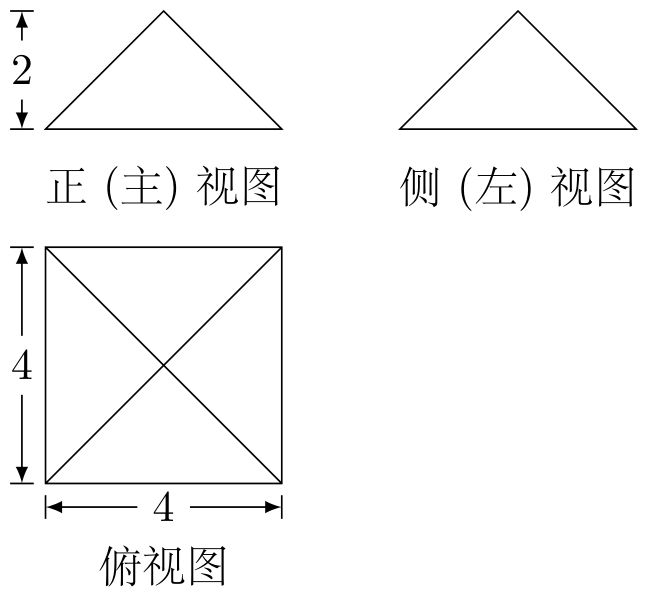
\includegraphics[width=6.3cm]{GaoKao/images/2011/beijing_liberal/q5_fig1.png}
\end{center}

        {\centering\begin{tabular*}{\linewidth}{@{}@{\extracolsep{\fill}}llll@{}}
          \text{A. }\(32\)  &  \text{B. }\(16 + 16\sqrt{2}\)  &  \text{C. }\(48\)  &  \text{D. }\(16 + 32\sqrt{2}\)
        \end{tabular*}\par}

        \item 执行如图所示的程序框图，若输入 \(A\) 的值为 2，则输出的 \(P\) 的值为（\quad）

\begin{center}
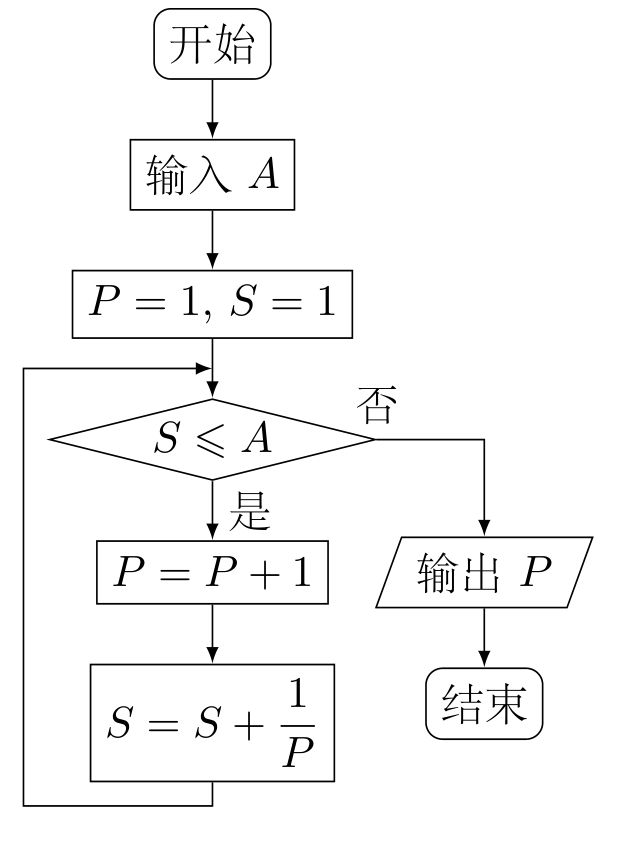
\includegraphics[width=0.38\linewidth]{GaoKao/images/2011/beijing_liberal/q6_fig1.png}
\end{center}

        {\centering\begin{tabular*}{\linewidth}{@{}@{\extracolsep{\fill}}llll@{}}
          \text{A. }\(2\)  &  \text{B. }\(3\)  &  \text{C. }\(4\)  &  \text{D. }\(5\)
        \end{tabular*}\par}

        \item 某车间分批生产某种产品，每批的生产准备费用为 \(800\text{ 元}\). 若每批生产 \(x\) 件，则平均仓储时间为 \(\frac{x}{8}\text{ 天}\)，且每件产品每天的仓储费用为 \(1\text{ 元}\). 为使平均到每件产品的生产准备费用与仓储费用之和最小，每批应生产产品（\quad）

        {\centering\begin{tabular*}{\linewidth}{@{}@{\extracolsep{\fill}}llll@{}}
          \text{A. }\(60\text{ 件}\)  &  \text{B. }\(80\text{ 件}\)  &  \text{C. }\(100\text{ 件}\)  &  \text{D. }\(120\text{ 件}\)
        \end{tabular*}\par}

        \item 已知点 \(A(0,2)\)，\(B(2,0)\). 若点 \(C\) 在函数 \(y = x^2\) 的图象上，则使得 \(\triangle ABC\) 的面积为 2 的点 \(C\) 的个数为（\quad）

        {\centering\begin{tabular*}{\linewidth}{@{}@{\extracolsep{\fill}}llll@{}}
          \text{A. }\(4\)  &  \text{B. }\(3\)  &  \text{C. }\(2\)  &  \text{D. }\(1\)
        \end{tabular*}\par}

    \end{enumerate}

\end{description}

\begin{description}

    \item[二、填空题]

    \begin{enumerate}[leftmargin=5pt]

      \addtocounter{enumi}{+8}

        \item 在 \(\triangle ABC\) 中，若 \(b = 5\)，\(\angle B = \frac{\pi}{4}\)，\(\sin A = \frac{1}{3}\)，则 \(a =\)\rule[-0.3ex]{3em}{0.4pt}.

        \item 已知双曲线 \(x^{2}-\frac{y^{2}}{b^{2}}=1\)（\(b>0\)）的一条渐近线的方程为 \(y = 2x\)，则 \(b=\)\rule[-0.3ex]{3em}{0.4pt}.

        \item 已知向量 \(\bm{a} = (\sqrt{3}, 1)\)，\(\bm{b} = (0, -1)\)，\(\bm{c} = (k, \sqrt{3})\). 若 \(\bm{a} - 2\bm{b}\) 与 \(\bm{c}\) 共线，则 \(k =\)\rule[-0.3ex]{3em}{0.4pt}.

        \item 在等比数列 \(\left\{a_{n}\right\}\) 中，\(a_{1}=\frac{1}{2}\)，\(a_{4}=-4\)，则公比 \(q=\)\rule[-0.3ex]{3em}{0.4pt}；\(a_{1}+a_{2}+\cdots+a_{n}=\)\rule[-0.3ex]{3em}{0.4pt}.

        \item 已知函数 \(f(x) = \begin{cases}
\dfrac{2}{x}, & x \geqslant 2,\\
(x - 1)^3, & x < 2,
\end{cases}\)
若关于 \(x\) 的方程 \(f(x) = k\) 有两个不同的实根，则实数 \(k\) 的取值范围是\rule[-0.3ex]{3em}{0.4pt}.

        \item 设 \(A(0,0)\)，\(B(4,0)\)，\(C(t + 4,3)\)，\(D(t,3) \)（\(t \in \mathbb{R}\)）. 记 \(N(t)\) 为平行四边形 \(ABCD\) 内部（不含边界）的整点的个数. 其中整点是指横，纵坐标都是整数的点，则 \(N(0) =\)\rule[-0.3ex]{3em}{0.4pt}；\(N(t)\) 的所有可能取值为\rule[-0.3ex]{3em}{0.4pt}.

    \end{enumerate}

\end{description}

\begin{description}

    \item[三、解答题]

    \begin{enumerate}[leftmargin=5pt]

      \addtocounter{enumi}{+14}

        \item 已知函数 \( f(x) = 4\cos x\sin \left(x + \frac{\pi}{6}\right) - 1 \).
\begin{enumerate}
\item 求 \( f(x) \) 的最小正周期.
\item 求 \( f(x) \) 在区间 \( \left[-\frac{\pi}{6}, \frac{\pi}{4}\right] \) 上的最大值和最小值.
\end{enumerate}

        \item 以下茎叶图记录了甲，乙两组各四名同学的植树棵数. 乙组记录中有一个数据模糊，无法确认，在图中以 \(X\) 表示.

\begin{center}
\begin{tabular}{r|c|l}
甲组 & & 乙组 \\
\hline
\(9\quad 9\) & 0 & \(X\quad 8\quad 9\) \\
\(1\quad 1\) & 1 & \(0\)
\end{tabular}
\end{center}

\begin{enumerate}
\item 如果 \(X = 8\)，求乙组同学植树棵数的平均数和方差；
\item 如果 \(X = 9\)，分别从甲，乙两组中随机选取一名同学，求这两名同学的植树总棵数为 19 的概率.
\end{enumerate}
（注：方差 \( s^2 = \frac{1}{n}\left[(x_1 - \overline{x})^2 + (x_2 - \overline{x})^2 + \ldots + (x_n - \overline{x})^2\right] \)，其中 \(\overline{x}\) 为 \(x_1\)，\(x_2\)，\(\cdots\)，\(x_n\) 的平均数）

        \item 如图，在四面体 \(PABC\) 中，\(PC \perp AB\)，\(PA \perp BC\)，点 \(D\)，\(E\)，\(F\)，\(G\) 分别是棱 \(AP\)，\(AC\)，\(BC\)，\(PB\) 的中点.

\begin{enumerate}
\item 求证：\(DE \parallel\) 平面 \(BCP\)；
\item 求证：四边形 \(DEFG\) 为矩形；
\item 是否存在点 \(Q\)，到四面体 \(PABC\) 六条棱的中点的距离相等？说明理由.
\end{enumerate}

\begin{center}
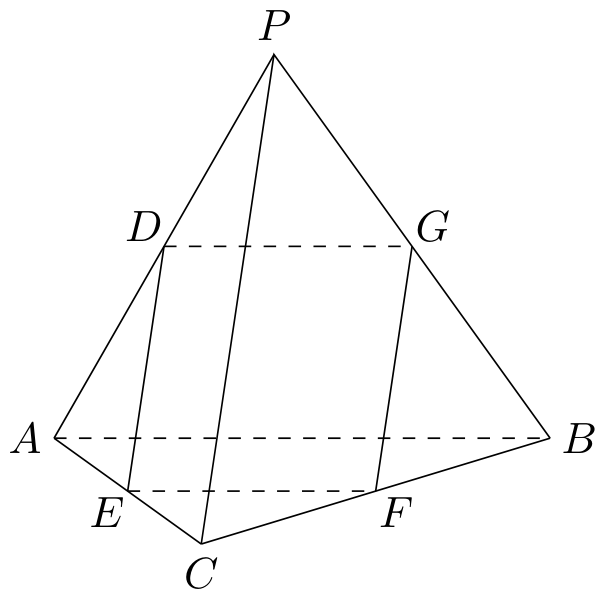
\includegraphics[width=7.5cm]{GaoKao/images/2011/beijing_liberal/q17_fig1.png}
\end{center}

        \item 已知函数 \( f(x) = (x - k){\mathrm{e}}^x \).
\begin{enumerate}
\item 求 \( f(x) \) 的单调区间；
\item 求 \( f(x) \) 在区间 \( [0,1] \) 上的最小值.
\end{enumerate}

        \item 已知椭圆 \(G: \frac{x^2}{a^{2}} + \frac{y^2}{b^{2}} = 1 \) （\(a > b > 0\)）的离心率为 \(\frac{\sqrt{6}}{3}\)，右焦点为 \((2\sqrt{2}, 0)\)，斜率为 1 的直线 \(l\) 与椭圆 \(G\) 交于 \(A\)，\(B\) 两点. 以 \(AB\) 为底边作等腰三角形，顶点为 \(P(-3, 2)\).
\begin{enumerate}
\item 求椭圆 \(G\) 的方程；
\item 求 \( \triangle PAB \) 的面积.
\end{enumerate}

        \item 若数列 \(A_{n}\)：\(a_{1}\)，\(a_{2}\)，\(\cdots\)，\(a_{n}\)（\(n \geqslant 2\)）满足 \(\left|a_{k+1} - a_{k}\right| = 1\)（\(k = 1, 2, \cdots, n-1\)），则称 \(A_{n}\) 为 \(E\) 数列. 记 \(S(A_{n}) = a_{1} + a_{2} + \cdots + a_{n}\).
\begin{enumerate}
\item 写出一个 \(E\) 数列 \(A_{n}\) 满足 \(a_{1}=a_{3}=0\)；
\item 若 \(a_1 = 12\)，\(n = 2000\)，证明：\(E\) 数列 \(A_n\) 是递增数列的充要条件是 \(a_n = 2011\)；
\item 在 \(a_1 = 4\) 的 \(E\) 数列 \(A_n\) 中，求使得 \(S(A_n) = 0\) 成立的 \(n\) 的最小值.
\end{enumerate}

    \end{enumerate}

\end{description}


\subsection{2011年重庆卷（理）}\label{gk:2011年重庆卷（理）}

\begin{description}

    \item[一、选择题]

    \begin{enumerate}[leftmargin=5pt]

        \item 复数 \(\frac{\i^2 + \i^3 + \i^4}{1 - \i} =\)（\quad）

        {\centering\begin{tabular*}{\linewidth}{@{}@{\extracolsep{\fill}}llll@{}}
          \text{A. }\(-\frac{1}{2} - \frac{1}{2}\i\)  &  \text{B. }\(-\frac{1}{2} + \frac{1}{2}\i\)  &  \text{C. }\(\frac{1}{2} - \frac{1}{2}\i\)  &  \text{D. }\(\frac{1}{2} + \frac{1}{2}\i\)
        \end{tabular*}\par}

        \item “\(x < -1\)”是“ \( x^{2} - 1 > 0 \) ”的（\quad）

        {\centering\begin{tabular*}{\linewidth}{@{}@{\extracolsep{\fill}}llll@{}}
          \text{A. }充分而不必要条件  &  \text{B. }必要而不充分条件  &  \text{C. }充要条件  &  \text{D. }既不充分也不必要条件
        \end{tabular*}\par}

        \item 已知 \(\lim\limits_{x\to +\infty}\left(\frac{2}{x - 1} + \frac{ax - 1}{3x}\right) = 2\)，则 \(a =\)（\quad）

        {\centering\begin{tabular*}{\linewidth}{@{}@{\extracolsep{\fill}}llll@{}}
          \text{A. }\(-6\)  &  \text{B. }2  &  \text{C. }3  &  \text{D. }6
        \end{tabular*}\par}

        \item \((1 + 3x)^{n}\) （其中 \(n\in \mathbb{N}\) 且 \(n\geqslant 6\) ）的展开式中 \(x^{5}\) 与 \(x^{6}\) 的系数相等，则（\quad）

        {\centering\begin{tabular*}{\linewidth}{@{}@{\extracolsep{\fill}}llll@{}}
          \text{A. }6  &  \text{B. }7  &  \text{C. }8  &  \text{D. }9
        \end{tabular*}\par}

        \item 下列区间中，函数 \( f(x) = |\ln (2 - x)| \) 在其上为增函数的是（\quad）

        {\centering\begin{tabular*}{\linewidth}{@{}@{\extracolsep{\fill}}llll@{}}
          \text{A. }\((-\infty, 1]\)  &  \text{B. }\(\left[-1, \frac{4}{3}\right]\)  &  \text{C. }\(\left[0, \frac{3}{2}\right)\)  &  \text{D. }\([1,2)\)
        \end{tabular*}\par}

        \item 若 \(\triangle ABC\) 的内角 \(A\)，\(B\)，\(C\) 所对的边 \(a\)，\(b\)，\(c\) 满足 \((a + b)^2 - c^2 = 4\)，且 \(C = 60^\circ\)，则 \(ab\) 的值为（\quad）

        {\centering\begin{tabular*}{\linewidth}{@{}@{\extracolsep{\fill}}llll@{}}
          \text{A. }\( \frac{4}{3} \)  &  \text{B. }\(8 - 4\sqrt{3}\)  &  \text{C. }1  &  \text{D. }\( \frac{2}{3} \)
        \end{tabular*}\par}

        \item 已知 \(a > 0\)，\(b > 0\)，\(a + b = 2\)，则 \(y = \frac{1}{a} + \frac{4}{b}\) 的最小值是（\quad）

        {\centering\begin{tabular*}{\linewidth}{@{}@{\extracolsep{\fill}}llll@{}}
          \text{A. }\( \frac{7}{2} \)  &  \text{B. }4  &  \text{C. }\( \frac{9}{2} \)  &  \text{D. }5
        \end{tabular*}\par}

        \item 在圆 \(x^{2} + y^{2} - 2x - 6y = 0\) 内，过点 \(E(0,1)\) 的最长弦和最短弦分别为 \(AC\) 和 \(BD\)，则四边形 \(ABCD\) 的面积为（\quad）

        {\centering\begin{tabular*}{\linewidth}{@{}@{\extracolsep{\fill}}llll@{}}
          \text{A. }\( 5\sqrt{2} \)  &  \text{B. }\(10\sqrt{2}\)  &  \text{C. }\(15\sqrt{2}\)  &  \text{D. }\(20\sqrt{2}\)
        \end{tabular*}\par}

        \item 高为 \(\frac{\sqrt{2}}{4}\) 的四棱锥 \(S - ABCD\) 的底面是边长为 1 的正方形，点 \(S\)，\(A\)，\(B\)，\(C\)，\(D\) 均在半径为 1 的同一球面上，则底面 \(ABCD\) 的中心与顶点 \(S\) 之间的距离为（\quad）

        {\centering\begin{tabular*}{\linewidth}{@{}@{\extracolsep{\fill}}llll@{}}
          \text{A. }\( \frac{\sqrt{2}}{4} \)  &  \text{B. }\( \frac{\sqrt{2}}{2} \)  &  \text{C. }1  &  \text{D. }\(\sqrt{2}\)
        \end{tabular*}\par}

        \item 设 \(m\)，\(k\) 为整数，方程 \(mx^2 - kx + 2 = 0\) 在区间 \((0,1)\) 内有两个不同的根，则 \(m + k\) 的最小值为（\quad）

        {\centering\begin{tabular*}{\linewidth}{@{}@{\extracolsep{\fill}}llll@{}}
          \text{A. }\(-8\)  &  \text{B. }8  &  \text{C. }12  &  \text{D. }13
        \end{tabular*}\par}

    \end{enumerate}

\end{description}

\begin{description}

    \item[二、填空题]

    \begin{enumerate}[leftmargin=5pt]

      \addtocounter{enumi}{+10}

        \item 在等差数列 \(\{a_{n}\}\) 中，\(a_{3} + a_{7} = 37\)，则 \(a_{2} + a_{4} + a_{6} + a_{8} =\rule[-0.3ex]{3em}{0.4pt}\).

        \item 已知单位向量 \(e_1\)，\(e_2\) 的夹角为 \(60^\circ\)，则 \(|2e_1 - e_2| =\rule[-0.3ex]{3em}{0.4pt}\).

        \item 将一枚均匀的硬币抛掷 6 次，则正面出现的次数比反面出现的次数多的概率为\rule[-0.3ex]{3em}{0.4pt}.

        \item 已知 \(\sin \alpha = \frac{1}{2} + \cos \alpha\)，且 \(\alpha \in \left(0, \frac{\pi}{2}\right)\)，则 \(\frac{\cos 2\alpha}{\sin \left(\alpha - \frac{\pi}{4}\right)}\) 的值为\rule[-0.3ex]{3em}{0.4pt}.

        \item 设圆 \(C\) 位于抛物线 \(y^{2} = 2x\) 与直线 \(x = 3\) 所围成的封闭区域（包含边界）内，则圆 \(C\) 的半径能取到的最大值为\rule[-0.3ex]{3em}{0.4pt}.

    \end{enumerate}

\end{description}

\begin{description}

    \item[三、解答题]

    \begin{enumerate}[leftmargin=5pt]

      \addtocounter{enumi}{+15}

        \item 设 \(a \in \mathbb{R}\)，\(f(x) = \cos x (a \sin x - \cos x) + \cos^2 \left(\frac{\pi}{2} - x\right)\) 满足 \(f\left(-\frac{\pi}{3}\right) = f(0)\)，求函数 \(f(x)\) 在 \(\left[\frac{\pi}{4}, \frac{11\pi}{24}\right]\) 上的最大值和最小值.

        \item 某市公租房的房源位于 \(A\)，\(B\)，\(C\) 三个片区. 设每位申请人只申请其中一个片区的房源. 且申请其中任一个片区的房源是等可能的. 求该市的任 \(4\) 位申请人中：
\begin{enumerate}
\item 恰有 2 人申请 \(A\) 片区的房源的概率；
\item 申请的房源所在片区的个数 \(\xi\) 的分布列与期望.
\end{enumerate}

        \item 设 \( f(x) = x^3 + ax^2 + bx + 1 \) 的导数 \( f'(x) \) 满足 \( f'(1) = 2a \)，\( f'(2) = -b \)，其中常数 \(a\)，\(b \in \mathbb{R}\).
\begin{enumerate}
\item 求曲线 \( y = f(x) \) 在点 \((1, f(1))\) 处的切线方程；
\item 设 \( g(x) = f'(x) {\mathrm{e}}^{-x} \)，求函数 \( g(x) \) 的极值.
\end{enumerate}

        \item 如图，在四面体 \(ABCD\) 中，平面 \(ABC \perp\) 平面 \(ACD\)，\(AB \perp BC\)，\(AD = CD\)，\(\angle CAD = 30^\circ\).
\begin{enumerate}
\item 若 \(AD = 2\)，\(AB = 2BC\)，求四面体 \(ABCD\) 的体积；
\item 若二面角 \(C - AB - D\) 为 \(60^{\circ}\)，求异面直线 \(AD\) 与 \(BC\) 所成角的余弦值.
\end{enumerate}

\begin{center}
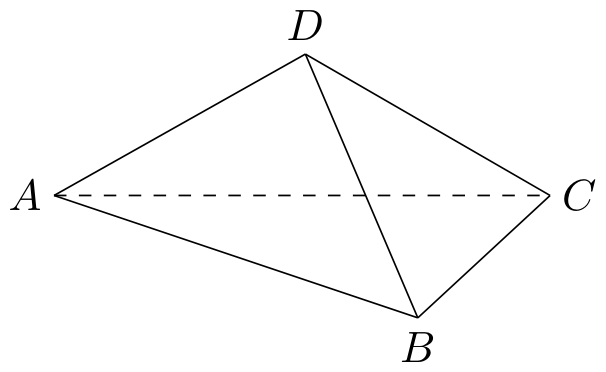
\includegraphics[width=7.5cm]{GaoKao/images/2011/chongqing_science/q19_fig1.png}
\end{center}

        \item 如图，椭圆的中心为原点 \(O\)，离心率 \(e = \frac{\sqrt{2}}{2}\)，一条准线的方程为 \(x = 2\sqrt{2}\).
\begin{enumerate}
\item 求该椭圆的标准方程；
\item 设动点 \(P\) 满足： \(\overrightarrow{OP} = \overrightarrow{OM} + 2\overrightarrow{ON}\)，其中 \(M\)，\(N\) 是椭圆上的点，直线 \(OM\) 与 \(ON\) 的斜率之积为 \(-\frac{1}{2}\). 问：是否存在两个定点 \(F_1\)，\(F_2\)，使得 \(|PF_1| + |PF_2|\) 为定值？若存在，求 \(F_1\)，\(F_2\) 的坐标；若不存在，说明理由.
\end{enumerate}

\begin{center}
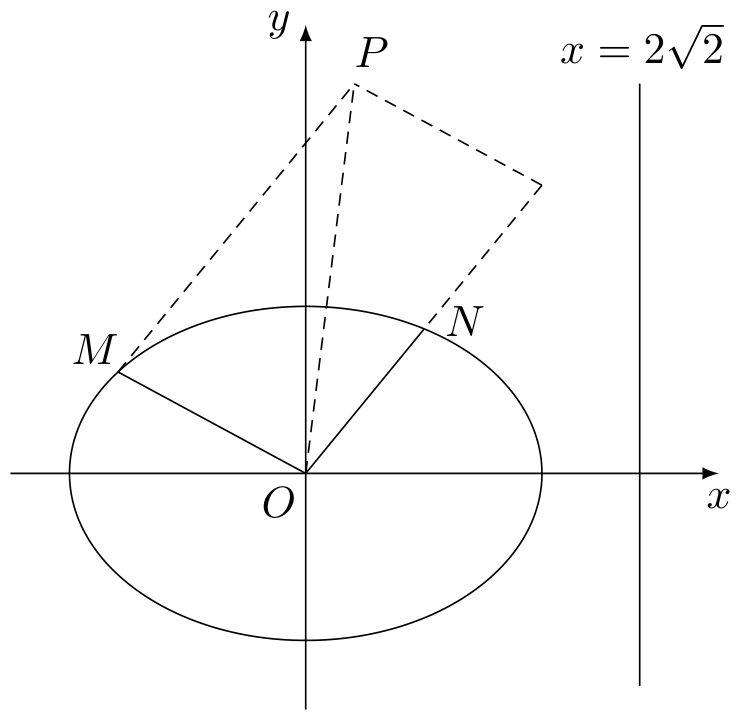
\includegraphics[width=8.9cm]{GaoKao/images/2011/chongqing_science/q20_fig1.png}
\end{center}

        \item 设实数数列 \(\{a_{n}\}\) 的前 \(n\) 项和 \(S_{n}\) 满足 \(S_{n + 1} = a_{n + 1}S_n\) （\(n\in \mathbb{N}^*\)）.
\begin{enumerate}
\item 若 \(a_{1}\)，\(S_{2}\)，\(-2a_{2}\) 成等比数列，求 \(S_{2}\) 和 \(a_{3}\)；
\item 求证：对 \(k \geqslant 3\) 有 \(0 \leqslant a_{k+1} \leqslant a_k \leqslant \frac{4}{3}\).
\end{enumerate}

    \end{enumerate}

\end{description}


\subsection{2011年重庆卷（文）}\label{gk:2011年重庆卷（文）}

\begin{description}

    \item[一、选择题]

    \begin{enumerate}[leftmargin=5pt]

        \item 在等差数列 \(\{a_{n}\}\) 中，\(a_{2} = 2\)，\(a_{3} = 4\)，则 \(a_{10} =\)（\quad）

        {\centering\begin{tabular*}{\linewidth}{@{}@{\extracolsep{\fill}}llll@{}}
          \text{A. }\(12\)  &  \text{B. }\(14\)  &  \text{C. }\(16\)  &  \text{D. }\(18\)
        \end{tabular*}\par}

        \item 设 \(U = \mathbb{R}\)，\(M = \{x \mid x^2 - 2x > 0\}\)，则 \(\complement_U M =\)（\quad）

        {\centering\begin{tabular*}{\linewidth}{@{}@{\extracolsep{\fill}}llll@{}}
          \text{A. }\(\left[0,2\right]\)  &  \text{B. }\(\left(0,2\right)\)  &  \text{C. }\(\left(-\infty,0\right)\cup\left(2,+\infty\right)\)  &  \text{D. }\(\left(-\infty,0\right]\cup\left[2,+\infty\right)\)
        \end{tabular*}\par}

        \item 曲线 \( y = -x^{3} + 3x^{2} \) 在点\(\left(1,2\right)\)处的切线方程为（\quad）

        {\centering\begin{tabular*}{\linewidth}{@{}@{\extracolsep{\fill}}llll@{}}
          \text{A. }\(y = 3x - 1\)  &  \text{B. }\(y = -3x + 5\)  &  \text{C. }\(y = 3x + 5\)  &  \text{D. }\(y = 2x\)
        \end{tabular*}\par}

        \item 从一堆苹果中任取 \(10\) 只，称得它们的质量如下（单位：\(\text{克}\)）：\(125\)，\(120\)，\(122\)，\(105\)，\(130\)，\(114\)，\(116\)，\(95\)，\(120\)，\(134\)，则样本数据落在 \(\left[114.5,124.5\right]\) 内的频率为（\quad）

        {\centering\begin{tabular*}{\linewidth}{@{}@{\extracolsep{\fill}}llll@{}}
          \text{A. }\(0.2\)  &  \text{B. }\(0.3\)  &  \text{C. }\(0.4\)  &  \text{D. }\(0.5\)
        \end{tabular*}\par}

        \item 已知向量 \(\bm{a} = (1, k)\)，\(\bm{b} = (2, 2)\)，且 \(\bm{a} + \bm{b}\) 与 \(\bm{a}\) 共线，那么 \(\bm{a} \cdot \bm{b}\) 的值为（\quad）

        {\centering\begin{tabular*}{\linewidth}{@{}@{\extracolsep{\fill}}llll@{}}
          \text{A. }\(1\)  &  \text{B. }\(2\)  &  \text{C. }\(3\)  &  \text{D. }\(4\)
        \end{tabular*}\par}

        \item 设 \(a = \log_{\frac{1}{3}} \frac{1}{2}\)，\(b = \log_{\frac{1}{3}} \frac{2}{3}\)，\(c = \log_3 \frac{4}{3}\)，则 \(a\)，\(b\)，\(c\) 的大小关系是（\quad）

        {\centering\begin{tabular*}{\linewidth}{@{}@{\extracolsep{\fill}}llll@{}}
          \text{A. }\(a < b < c\)  &  \text{B. }\(c < b < a\)  &  \text{C. }\(b < a < c\)  &  \text{D. }\(b < c < a\)
        \end{tabular*}\par}

        \item 若函数 \( f(x) = x + \frac{1}{x - 2} \)（\(x > 2\)）在 \( x = a \) 处取最小值，则 \( a = \)（\quad）

        {\centering\begin{tabular*}{\linewidth}{@{}@{\extracolsep{\fill}}llll@{}}
          \text{A. }\(1 + \sqrt{2}\)  &  \text{B. }\(1 + \sqrt{3}\)  &  \text{C. }\(3\)  &  \text{D. }\(4\)
        \end{tabular*}\par}

        \item 若 \(\triangle ABC\) 的内角 \(A\)，\(B\)，\(C\) 满足 \(6\sin A = 4\sin B = 3\sin C\)，则 \(\cos B =\)（\quad）

        {\centering\begin{tabular*}{\linewidth}{@{}@{\extracolsep{\fill}}llll@{}}
          \text{A. }\(\frac{\sqrt{15}}{4}\)  &  \text{B. }\(\frac{3}{4}\)  &  \text{C. }\(\frac{3\sqrt{15}}{16}\)  &  \text{D. }\(\frac{11}{16}\)
        \end{tabular*}\par}

        \item 设双曲线的左准线与两条渐近线交于 \(A\)，\(B\) 两点，左焦点在以 \(AB\) 为直径的圆内，则该双曲线的离心率取值范围为（\quad）

        {\centering\begin{tabular*}{\linewidth}{@{}@{\extracolsep{\fill}}llll@{}}
          \text{A. }\(\left(0,\sqrt{2}\right)\)  &  \text{B. }\(\left(1,\sqrt{2}\right)\)  &  \text{C. }\(\left(\frac{\sqrt{2}}{2}, 1\right)\)  &  \text{D. }\(\left(\sqrt{2},+\infty\right)\)
        \end{tabular*}\par}

        \item 高为 \(\sqrt{2}\) 的四棱锥 \(S - ABCD\) 的底面是边长为 \(1\) 的正方形，点 \(S\)，\(A\)，\(B\)，\(C\)，\(D\) 均在半径为 \(1\) 的同一球面上，则底面 \(ABCD\) 的中心与顶点 \(S\) 之间的距离为（\quad）

        {\centering\begin{tabular*}{\linewidth}{@{}@{\extracolsep{\fill}}llll@{}}
          \text{A. }\(\frac{\sqrt{10}}{2}\)  &  \text{B. }\(\frac{\sqrt{2} + \sqrt{3}}{2}\)  &  \text{C. }\(\frac{3}{2}\)  &  \text{D. }\(\sqrt{2}\)
        \end{tabular*}\par}

    \end{enumerate}

\end{description}

\begin{description}

    \item[二、填空题]

    \begin{enumerate}[leftmargin=5pt]

      \addtocounter{enumi}{+10}

        \item \(\left(1 + 2x\right)^{6}\) 的展开式中 \(x^{4}\) 的系数是\rule[-0.3ex]{3em}{0.4pt}.

        \item 若 \(\cos \alpha = -\frac{3}{5}\)，且 \(\alpha \in \left(\pi, \frac{3\pi}{2}\right)\)，则 \(\tan \alpha =\)\rule[-0.3ex]{3em}{0.4pt}.

        \item 过原点的直线与圆 \(x^{2} + y^{2} - 2x - 4y + 4 = 0\) 相交所得弦的长为\(2\)，则该直线的方程为\rule[-0.3ex]{3em}{0.4pt}.

        \item 从甲，乙等\(10\)位同学中任选\(3\)位去参加某项活动，则所选\(3\)位中有甲但没有乙的概率为\rule[-0.3ex]{3em}{0.4pt}.

        \item 若实数 \(a\)，\(b\)，\(c\) 满足 \(2^{a} + 2^{b} = 2^{a + b}\)，\(2^{a} + 2^{b} + 2^{c} = 2^{a + b + c}\)，则 \(c\) 的最大值是\rule[-0.3ex]{3em}{0.4pt}.

    \end{enumerate}

\end{description}

\begin{description}

    \item[三、解答题]

    \begin{enumerate}[leftmargin=5pt]

      \addtocounter{enumi}{+15}

        \item 设 \(\{a_{n}\}\) 是公比为正数的等比数列，\(a_{1} = 2\)，\(a_{3} = a_{2} + 4\).
\begin{enumerate}
\item 求 \( \{a_{n}\} \) 的通项公式；
\item 设 \( \{b_{n}\} \) 是首项为 1，公差为 2 的等差数列. 求数列 \( \{a_{n} + b_{n}\} \) 的前 \(n\) 项和 \(S_{n}\).
\end{enumerate}

        \item 某市公租房的房源位于 \(A\)，\(B\)，\(C\) 三个片区. 设每位申请人只申请其中一个片区的房源，且申请其中任一个片区的房源是等可能的，求该市的任 \(4\) 位申请人中：
\begin{enumerate}
\item 没有人申请 \(A\) 片区房源的概率；
\item 每个片区的房源都有人申请的概率.
\end{enumerate}

        \item 设函数 \(f(x) = \sin x \cos x - \sqrt{3}\cos\left(\pi + x\right)\cos x\) （\(x \in \mathbb{R}\)）.
\begin{enumerate}
\item 求 \(f(x)\) 的最小正周期；
\item 若函数 \(y = f(x)\) 的图象按 \(\bm{b} = \left(\frac{\pi}{4}, \frac{\sqrt{3}}{2}\right)\) 平移后得到函数 \(y = g(x)\) 的图象，求 \(y = g(x)\) 在 \(\left[0, \frac{\pi}{4}\right]\) 上的最大值.
\end{enumerate}

        \item 设 \( f(x) = 2x^{3} + ax^{2} + bx + 1 \) 的导数为 \( f'(x) \). 若函数 \( y = f'(x) \) 的图象关于直线 \( x = -\frac{1}{2} \) 对称，且 \( f'(1) = 0 \).
\begin{enumerate}
\item 求实数 \(a\)，\(b\) 的值；
\item 求函数 \( f(x) \) 的极值.
\end{enumerate}

        \item 如图，在四面体 \(ABCD\) 中，平面 \(ABC \perp\) 平面 \(ACD\)，\(AB \perp BC\)，\(AC = AD = 2\)，\(BC = CD = 1\).
\begin{enumerate}
\item 求四面体 \(ABCD\) 的体积；
\item 求二面角 \(C - AB - D\) 的平面角的正切值.
\end{enumerate}
\begin{center}
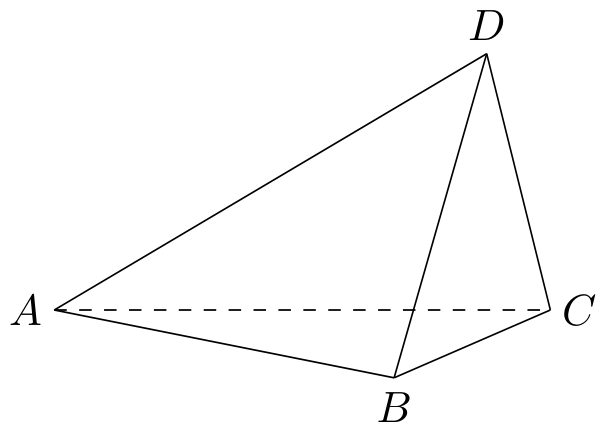
\includegraphics[width=7.5cm]{GaoKao/images/2011/chongqing_liberal/q20_fig1.png}
\end{center}

        \item 如图，椭圆的中心为原点 \(O\)，离心率 \( e = \frac{\sqrt{2}}{2} \)，一条准线的方程是 \( x = 2\sqrt{2} \).
\begin{enumerate}
\item 求该椭圆的标准方程；
\item 设动点 \(P\) 满足： \(\overrightarrow{OP} = \overrightarrow{OM} + 2\overrightarrow{ON}\)，其中 \(M\)，\(N\) 是椭圆上的点，直线 \(OM\) 与 \(ON\) 的斜率之积为 \(-\frac{1}{2}\)，问：是否存在定点 \(F\)，使得 \(|PF|\) 与点 \(P\) 到直线 \(l: x = 2\sqrt{10}\) 的距离之比为定值？ 若存在，求 \(F\) 的坐标；若不存在，说明理由.
\end{enumerate}
\begin{center}
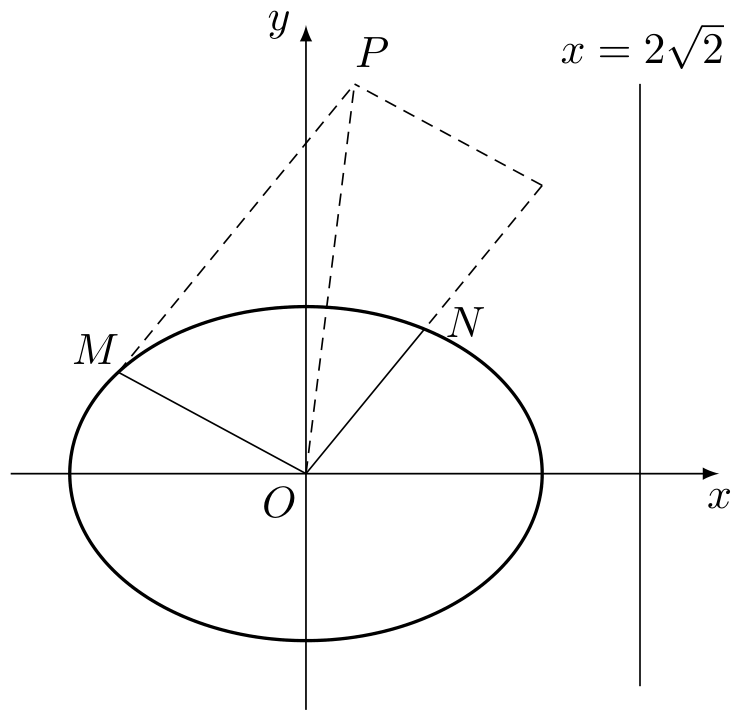
\includegraphics[width=9.3cm]{GaoKao/images/2011/chongqing_liberal/q21_fig1.png}
\end{center}

    \end{enumerate}

\end{description}


\subsection{2011年福建卷（理）}\label{gk:2011年福建卷（理）}

\begin{description}

    \item[一、选择题]

    \begin{enumerate}[leftmargin=5pt]

        \item \(\i\) 是虚数单位，若集合 \(S = \{-1, 0, 1\}\)，则（\quad）

        {\centering\begin{tabular*}{\linewidth}{@{}@{\extracolsep{\fill}}llll@{}}
          \text{A. }\(\i \in S\)  &  \text{B. }\(\i^2\in S\)  &  \text{C. }\(\i^3\in S\)  &  \text{D. }\(\frac{2}{\i} \in S\)
        \end{tabular*}\par}

        \item 若 \(a \in \mathbb{R}\)，则 “\(a = 2\)” 是 “\((a - 1)(a - 2) = 0\)” 的（\quad）

        {\centering\begin{tabular*}{\linewidth}{@{}@{\extracolsep{\fill}}llll@{}}
          \text{A. }充分而不必要条件  &  \text{B. }必要而不充分条件  &  \text{C. }充要条件  &  \text{D. }既不充分也不必要条件
        \end{tabular*}\par}

        \item 若 \(\tan \alpha = 3\)，则 \(\frac{\sin 2\alpha}{\cos^2 \alpha}\) 的值等于（\quad）

        {\centering\begin{tabular*}{\linewidth}{@{}@{\extracolsep{\fill}}llll@{}}
          \text{A. }2  &  \text{B. }3  &  \text{C. }4  &  \text{D. }6
        \end{tabular*}\par}

        \item 如图，矩形 \(ABCD\) 中，点 \(E\) 为边 \(CD\) 的中点，若在矩形 \(ABCD\) 内部随机取一个点 \(Q\)，则点 \(Q\) 取自 \(\triangle ABE\) 内部的概率等于（\quad）

\begin{center}
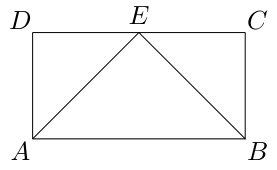
\includegraphics[width=5.7cm]{GaoKao/images/2011/fujian_science/q4_fig1.png}
\end{center}

        {\centering\begin{tabular*}{\linewidth}{@{}@{\extracolsep{\fill}}llll@{}}
          \text{A. }\( \frac{1}{4} \)  &  \text{B. }\( \frac{1}{3} \)  &  \text{C. }\( \frac{1}{2} \)  &  \text{D. }\( \frac{2}{3} \)
        \end{tabular*}\par}

        \item \(\int_{0}^{1}\left({\mathrm{e}}^{x} + 2x\right)\mathrm{d}x\) 等于（\quad）

        {\centering\begin{tabular*}{\linewidth}{@{}@{\extracolsep{\fill}}llll@{}}
          \text{A. }1  &  \text{B. }\({\mathrm{e}}\) - 1  &  \text{C. }\({\mathrm{e}}\)  &  \text{D. }\({\mathrm{e}}\) + 1
        \end{tabular*}\par}

        \item \((1 + 2x)^{5}\) 的展开式中，\(x^{2}\) 的系数等于（\quad）

        {\centering\begin{tabular*}{\linewidth}{@{}@{\extracolsep{\fill}}llll@{}}
          \text{A. }80  &  \text{B. }40  &  \text{C. }20  &  \text{D. }10
        \end{tabular*}\par}

        \item 设圆锥曲线 \(T\) 的两个焦点分别为 \(F_{1}\)，\(F_{2}\). 若曲线 \(T\) 上存在点 \(P\) 满足 \(|PF_{1}|: |F_{1}F_{2}|: |PF_{2}| = 4:3:2\)，则曲线 \(T\) 的离心率等于（\quad）

        {\centering\begin{tabular*}{\linewidth}{@{}@{\extracolsep{\fill}}llll@{}}
          \text{A. }\(\frac{1}{2}\) 或 \(\frac{3}{2}\)  &  \text{B. }\(\frac{2}{3}\) 或 2  &  \text{C. }\(\frac{1}{2}\) 或 2  &  \text{D. }\(\frac{2}{3}\) 或 \(\frac{3}{2}\)
        \end{tabular*}\par}

        \item 已知 \(O\) 是坐标原点，点 \(A(-1,1)\)，若点 \(M(x,y)\) 为平面区域 \(\begin{cases}
x+y\geqslant 2,\\
x\leqslant 1,\\
y\leqslant 2
\end{cases}\) 上的一个动点，则 \(\overrightarrow{OA}\cdot\overrightarrow{OM}\) 的取值范围是（\quad）

        {\centering\begin{tabular*}{\linewidth}{@{}@{\extracolsep{\fill}}llll@{}}
          \text{A. }\([-1,0]\)  &  \text{B. }\([0,1]\)  &  \text{C. }\([0,2]\)  &  \text{D. }\([-1,2]\)
        \end{tabular*}\par}

        \item 对于函数 \(f(x)=a\sin x+bx+c\)（其中 \(a\)，\(b\in\mathbb{R}\)，\(c\in\mathbb{Z}\)），选取 \(a\)，\(b\)，\(c\) 的一组值计算 \(f(1)\) 和 \(f(-1)\)，所得出的正确结果一定不可能是（\quad）

        {\centering\begin{tabular*}{\linewidth}{@{}@{\extracolsep{\fill}}llll@{}}
          \text{A. }4 和 6  &  \text{B. }3 和 1  &  \text{C. }2 和 4  &  \text{D. }1 和 2
        \end{tabular*}\par}

        \item 已知函数 \(f(x)={\mathrm{e}}^{x}+x\). 对于曲线 \(y=f(x)\) 上横坐标成等差数列的三个点 \(A\)，\(B\)，\(C\)，给出以下判断：

\begin{enumerate}
\item \(\triangle ABC\) 一定是钝角三角形；
\item \(\triangle ABC\) 可能是直角三角形；
\item \(\triangle ABC\) 可能是等腰三角形；
\item \(\triangle ABC\) 不可能是等腰三角形.
\end{enumerate}

其中，正确的判断是（\quad）

        {\centering\begin{tabular*}{\linewidth}{@{}@{\extracolsep{\fill}}llll@{}}
          \text{A. }\ding{172}\ding{174}  &  \text{B. }\ding{172}\ding{175}  &  \text{C. }\ding{173}\ding{174}  &  \text{D. }\ding{173}\ding{175}
        \end{tabular*}\par}

    \end{enumerate}

\end{description}

\begin{description}

    \item[二、填空题]

    \begin{enumerate}[leftmargin=5pt]

      \addtocounter{enumi}{+10}

        \item 运行如图所示的程序，输出的结果是\rule[-0.3ex]{3em}{0.4pt}.

\begin{center}
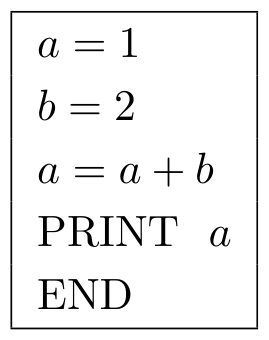
\includegraphics[width=3.3cm]{GaoKao/images/2011/fujian_science/q11_fig1.png}
\end{center}

        \item 三棱锥 \(P - ABC\) 中，\(PA \perp\) 底面 \(ABC\)，\(PA = 3\)，底面 \(ABC\) 是边长为 \(2\) 的正三角形，则三棱锥 \(P - ABC\) 的体积等于\rule[-0.3ex]{3em}{0.4pt}.

        \item 盒中装有形状，大小完全相同的 \(5\) 个球，其中红色球 \(3\) 个，黄色球 \(2\) 个. 若从中随机取出 \(2\) 个球，则所取出的 \(2\) 个球颜色不同的概率等于\rule[-0.3ex]{3em}{0.4pt}.

        \item 如图，\(\triangle ABC\) 中，\(AB = AC = 2\)，\(BC = 2\sqrt{3}\)，点 \(D\) 在 \(BC\) 边上，\(\angle ADC = 45^\circ\)，则 \(AD\) 的长度等于\rule[-0.3ex]{3em}{0.4pt}.

\begin{center}
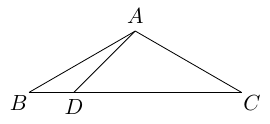
\includegraphics[width=6.5cm]{GaoKao/images/2011/fujian_science/q14_fig1.png}
\end{center}

        \item 设 \(V\) 是全体平面向量构成的集合. 若映射 \(f:V\to\mathbb{R}\) 满足：对任意向量 \(a=(x_1,y_1)\in V\)，\(b=(x_2,y_2)\in V\)，以及任意 \(\lambda\in\mathbb{R}\)，均有 \(f\left(\lambda a+(1-\lambda)b\right)=\lambda f(a)+(1-\lambda)f(b)\)，则称映射 \(f\) 具有性质 \(P\). 现给出如下映射：

\begin{enumerate}
\item \(f_1:V\to\mathbb{R}\)，\(f_1(m)=x-y\)，\(m=(x,y)\in V\)；
\item \(f_2:V\to\mathbb{R}\)，\(f_2(m)=x^2+y\)，\(m=(x,y)\in V\)；
\item \(f_3:V\to\mathbb{R}\)，\(f_3(m)=x+y+1\)，\(m=(x,y)\in V\).
\end{enumerate}

其中，具有性质 \(P\) 的映射的序号为\rule[-0.3ex]{3em}{0.4pt}（写出所有具有性质 \(P\) 的映射的序号）.

    \end{enumerate}

\end{description}

\begin{description}

    \item[三、解答题]

    \begin{enumerate}[leftmargin=5pt]

      \addtocounter{enumi}{+15}

        \item 已知等比数列 \(\{a_n\}\) 的公比 \(q=3\)，前 \(3\) 项和 \(S_3=\frac{13}{3}\).

\begin{enumerate}
\item 求数列 \(\{a_n\}\) 的通项公式；
\item 若函数 \(f(x)=A\sin\left(2x+\varphi\right)\)（\(A>0\)，\(0<\varphi<\pi\)）在 \(x=\frac{\pi}{6}\) 处取得最大值，且最大值为 \(a_3\)，求函数 \(f(x)\) 的解析式.
\end{enumerate}

        \item 已知直线 \(l:y=x+m\)，\(m\in\mathbb{R}\).

\begin{enumerate}
\item 若以点 \(M(2,0)\) 为圆心的圆与直线 \(l\) 相切于点 \(P\)，且点 \(P\) 在 \(y\) 轴上，求该圆的方程；
\item 若直线 \(l\) 关于 \(x\) 轴对称的直线为 \(l'\)，问直线 \(l'\) 与抛物线 \(C:x^2=4y\) 是否相切？说明理由.
\end{enumerate}

        \item 某商场销售某种商品的经验表明，该商品每日的销售量 \(y\)（单位：千克）与销售价格 \(x\)（单位：元/千克）满足关系式 \(y=\frac{a}{x-3}+10(x-6)^2\)，其中 \(3<x<6\)，\(a\) 为常数. 已知销售价格为 \(5\text{ 元/千克}\) 时，每日可售出该商品 \(11\text{ 千克}\).

\begin{enumerate}
\item 求 \(a\) 的值；
\item 若该商品的成本为 \(3\text{ 元/千克}\)，试确定销售价格 \(x\) 的值，使商场每日销售该商品所获得的利润最大.
\end{enumerate}

        \item 某产品按行业生产标准分成 \(8\) 个等级，等级系数 \(X\) 依次为 \(1\)，\(2\)，\(\dots\)，\(8\)，其中 \(X\geqslant 5\) 为标准 \(A\)，\(X\geqslant 3\) 为标准 \(B\). 已知甲厂执行标准 \(A\) 生产该产品，产品的零售价为 \(6\text{ 元/件}\)；乙厂执行标准 \(B\) 生产该产品，产品的零售价为 \(4\text{ 元/件}\)，假定甲，乙两厂的产品都符合相应的执行标准.

\begin{enumerate}
\item 已知甲厂产品的等级系数 \(X_1\) 的概率分布如下表所示：

\begin{center}
\begin{tabular}{|c|c|c|c|c|}
\hline
\(X_1\) & 5 & 6 & 7 & 8 \\
\hline
\(P\) & 0.4 & \(a\) & \(b\) & 0.1 \\
\hline
\end{tabular}
\end{center}

且 \(E(X_1)=6\). 求 \(a\)，\(b\) 的值；
\item 为分析乙厂产品的等级系数 \(X_2\)，从该厂生产的产品中随机抽取 \(30\) 件，相应的等级系数组成一个样本. 数据如下：

\begin{center}
\begin{tabular}{cccccccccc}
3 & 5 & 3 & 3 & 8 & 5 & 5 & 6 & 3 & 4 \\
6 & 3 & 4 & 7 & 5 & 3 & 4 & 8 & 5 & 3 \\
8 & 3 & 4 & 3 & 4 & 4 & 7 & 5 & 6 & 7
\end{tabular}
\end{center}

用这个样本的频率分布估计总体分布，将频率视为概率，求等级系数 \(X_2\) 的数学期望；
\item 在前两问的条件下，若以“性价比”为判断标准，则哪个工厂的产品更具可购买性？说明理由.
\end{enumerate}

注：

\begin{enumerate}
\item 产品的“性价比”\(=\frac{\text{产品的等级系数的数学期望}}{\text{产品的零售价}}\)；
\item “性价比”大的产品更具可购买性.
\end{enumerate}

        \item 如图，四棱锥 \(P-ABCD\) 中，\(PA\perp\) 底面 \(ABCD\)，四边形 \(ABCD\) 中，\(AB\perp AD\)，\(AB+AD=4\)，\(CD=\sqrt{2}\)，\(\angle CDA=45^\circ\).

\begin{enumerate}
\item 求证：平面 \(PAB\perp\) 平面 \(PAD\)；
\item 设 \(AB=AP\).

\begin{enumerate}
\item 若直线 \(PB\) 与平面 \(PCD\) 所成的角为 \(30^\circ\)，求线段 \(AB\) 的长；
\item 在线段 \(AD\) 上是否存在一个点 \(G\)，使得点 \(G\) 到点 \(P\)，\(B\)，\(C\)，\(D\) 的距离都相等？说明理由.
\end{enumerate}
\end{enumerate}

\begin{center}
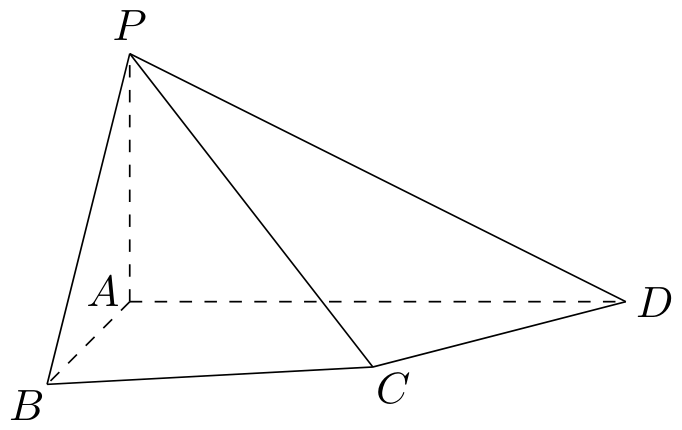
\includegraphics[width=8.5cm]{GaoKao/images/2011/fujian_science/q20_fig1.png}
\end{center}

    \end{enumerate}

\end{description}

\begin{description}

    \item[四、选考题]

    \begin{enumerate}[leftmargin=5pt]

      \addtocounter{enumi}{+20}

        \item 设矩阵 \(M = \begin{pmatrix} a & 0 \\ 0 & b \end{pmatrix}\)（其中 \(a > 0\)，\(b > 0\)）

\begin{enumerate}
\item 若 \(a = 2\)，\(b = 3\)，求矩阵 \(M\) 的逆矩阵 \(M^{-1}\)；
\item 若曲线 \(C: x^{2} + y^{2} = 1\) 在矩阵 \(M\) 所对应的线性变换作用下得到曲线
\(C' : \frac{x^{2}}{4} + y^{2} = 1\)，求 \(a\)，\(b\) 的值.
\end{enumerate}

        \item \textbf{【选修4-4：坐标系与参数方程】}

在直角坐标系 \(xOy\) 中，直线 \(l\) 的方程为 \(x-y+4=0\)，曲线 \(C\) 的参数方程为 \(\begin{cases}
x=\sqrt{3}\cos\alpha,\\
y=\sin\alpha
\end{cases}\)（\(\alpha\) 为参数）.

\begin{enumerate}
\item 已知在极坐标（与直角坐标系 \(xOy\) 取相同的长度单位，且以原点 \(O\) 为极点，以 \(x\) 轴正半轴为极轴）中，点 \(P\) 的极坐标为 \(\left(4,\frac{\pi}{2}\right)\)，判断点 \(P\) 与直线 \(l\) 的位置关系；
\item 设点 \(Q\) 是曲线 \(C\) 上的一个动点，求它到直线 \(l\) 的距离的最小值.
\end{enumerate}

        \item \textbf{【选修4-5：不等式选讲】}

设不等式 \(|2x-1|<1\) 的解集为 \(M\).

\begin{enumerate}
\item 求集合 \(M\)；
\item 若 \(a\)，\(b\in M\)，试比较 \(ab+1\) 与 \(a+b\) 的大小.
\end{enumerate}

    \end{enumerate}

\end{description}


\subsection{2011年福建卷（文）}\label{gk:2011年福建卷（文）}

\begin{description}

    \item[一、选择题]

    \begin{enumerate}[leftmargin=5pt]

        \item 若集合 \(M = \{-1, 0, 1\}\)，\(N = \{0, 1, 2\}\)，则 \(M \cap N\) 等于（\quad）

        {\centering\begin{tabular*}{\linewidth}{@{}@{\extracolsep{\fill}}llll@{}}
          \text{A. }\(\{0, 1\}\)  &  \text{B. }\( \{-1,0,1\} \)  &  \text{C. }\(\{0,1,2\}\)  &  \text{D. }\(\{-1,0,1,2\}\)
        \end{tabular*}\par}

        \item \(\i\) 是虚数单位，\( 1 + \i^{3} \) 等于（\quad）

        {\centering\begin{tabular*}{\linewidth}{@{}@{\extracolsep{\fill}}llll@{}}
          \text{A. }\(\i\)  &  \text{B. }\(-\i\)  &  \text{C. }\(1 + \i\)  &  \text{D. }\(1 - \i\)
        \end{tabular*}\par}

        \item 若 \(a \in \mathbb{R}\)，则“\(a = 1\)”是“\(\lvert a \rvert = 1\)”的（\quad）

        {\centering\begin{tabular*}{\linewidth}{@{}@{\extracolsep{\fill}}llll@{}}
          \text{A. }充分而不必要条件  &  \text{B. }必要而不充分条件  &  \text{C. }充要条件  &  \text{D. }既不充分也不必要条件
        \end{tabular*}\par}

        \item 某校选修乒乓球课程的学生中，高一年级有 30 名，高二年级有 40 名. 现用分层抽样的方法在这 70 名学生中抽取一个样本，已知在高一年级的学生中抽取了 6 名，则在高二年级的学生中应抽取的人数为（\quad）

        {\centering\begin{tabular*}{\linewidth}{@{}@{\extracolsep{\fill}}llll@{}}
          \text{A. }6  &  \text{B. }8  &  \text{C. }10  &  \text{D. }12
        \end{tabular*}\par}

        \item 阅读如图所示的程序框图，运行相应的程序，输出的结果是（\quad）

\begin{center}
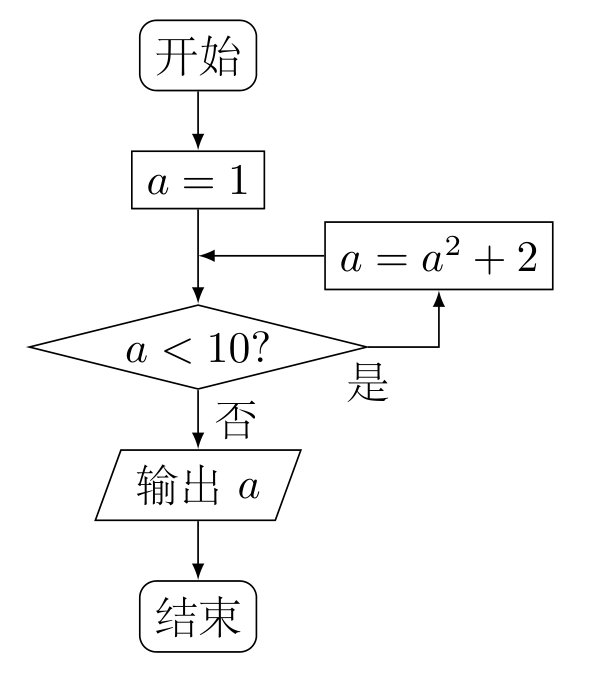
\includegraphics[width=0.34\linewidth]{GaoKao/images/2011/fujian_liberal/q5_fig1.png}
\end{center}

        {\centering\begin{tabular*}{\linewidth}{@{}@{\extracolsep{\fill}}llll@{}}
          \text{A. }3  &  \text{B. }11  &  \text{C. }38  &  \text{D. }123
        \end{tabular*}\par}

        \item 若关于 \(x\) 的方程 \(x^{2} + mx + 1 = 0\) 有两个不相等的实数根，则实数 \(m\) 的取值范围是（\quad）

        {\centering\begin{tabular*}{\linewidth}{@{}@{\extracolsep{\fill}}llll@{}}
          \text{A. }\((-1, 1)\)  &  \text{B. }\((-2, 2)\)  &  \text{C. }\((- \infty, -2) \cup (2, +\infty)\)  &  \text{D. }\((-\infty, -1) \cup (1, +\infty)\)
        \end{tabular*}\par}

        \item 如图，矩形 \(ABCD\) 中，点 \(E\) 为边 \(CD\) 的中点，若在矩形 \(ABCD\) 内部随机取一个点 \(Q\)，则点 \(Q\) 取自 \(\triangle ABE\) 内部的概率等于（\quad）

\begin{center}
\begin{center}
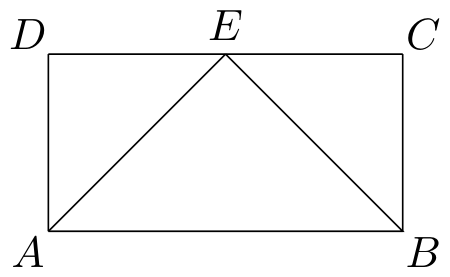
\includegraphics[width=5.6cm]{GaoKao/images/2011/fujian_liberal/q7_fig1.png}
\end{center}
\end{center}

        {\centering\begin{tabular*}{\linewidth}{@{}@{\extracolsep{\fill}}llll@{}}
          \text{A. }\( \frac{1}{4} \)  &  \text{B. }\( \frac{1}{3} \)  &  \text{C. }\( \frac{1}{2} \)  &  \text{D. }\( \frac{2}{3} \)
        \end{tabular*}\par}

        \item 已知函数 \( f(x) = \begin{cases}
2^x, & x > 0,\\
x + 1, & x \leqslant 0.
\end{cases} \) 若 \( f(a) + f(1) = 0 \)，则实数 \( a \) 的值等于（\quad）

        {\centering\begin{tabular*}{\linewidth}{@{}@{\extracolsep{\fill}}llll@{}}
          \text{A. }\(-3\)  &  \text{B. }\(-1\)  &  \text{C. }1  &  \text{D. }3
        \end{tabular*}\par}

        \item 若 \(\alpha \in \left(0, \frac{\pi}{2}\right)\)，且 \(\sin^2\alpha + \cos 2\alpha = \frac{1}{4}\)，则 \(\tan \alpha\) 的值等于（\quad）

        {\centering\begin{tabular*}{\linewidth}{@{}@{\extracolsep{\fill}}llll@{}}
          \text{A. }\(\frac{\sqrt{2}}{2}\)  &  \text{B. }\( \frac{\sqrt{3}}{3} \)  &  \text{C. }\(\sqrt{2}\)  &  \text{D. }\(\sqrt{3}\)
        \end{tabular*}\par}

        \item 若 \(a > 0\)，\(b > 0\)，且函数 \(f(x) = 4x^3 - ax^2 - 2bx + 2\) 在 \(x = 1\) 处有极值，则 \(ab\) 的最大值等于（\quad）

        {\centering\begin{tabular*}{\linewidth}{@{}@{\extracolsep{\fill}}llll@{}}
          \text{A. }2  &  \text{B. }3  &  \text{C. }6  &  \text{D. }9
        \end{tabular*}\par}

        \item 设圆锥曲线 \(\Gamma\) 的两个焦点分别为 \(F_{1}\)，\(F_{2}\). 若曲线 \(\Gamma\) 上存在点 \(P\) 满足 \(|PF_{1}|: |F_{1}F_{2}|: |PF_{2}| = 4:3:2\)，则曲线 \(\Gamma\) 的离心率等于（\quad）

        {\centering\begin{tabular*}{\linewidth}{@{}@{\extracolsep{\fill}}llll@{}}
          \text{A. }\(\frac{1}{2}\) 或 \(\frac{3}{2}\)  &  \text{B. }\(\frac{2}{3}\) 或 2  &  \text{C. }\(\frac{1}{2}\) 或 2  &  \text{D. }\(\frac{2}{3}\) 或 \(\frac{3}{2}\)
        \end{tabular*}\par}

        \item 在整数集 \(\mathbb{Z}\) 中，被 5 除所得余数为 \(k\) 的所有整数组成一个“类”，记为 \([k]\)，即 \([k] = \{5n + k \mid n \in \mathbb{Z}\}\)，\(k = 0\)，\(1\)，\(2\)，\(3\)，\(4\). 给出如下四个结论：

\begin{enumerate}
\item \(2011 \in [1]\)；
\item \(-3 \in [3]\)；
\item \(\mathbb{Z} = [0] \cup [1] \cup [2] \cup [3] \cup [4]\)；
\item “整数 \(a\)，\(b\) 属于同一‘类’”的充要条件是 “\(a - b \in [0]\)”.
\end{enumerate}

其中，正确结论的个数是（\quad）

        {\centering\begin{tabular*}{\linewidth}{@{}@{\extracolsep{\fill}}llll@{}}
          \text{A. }1  &  \text{B. }2  &  \text{C. }3  &  \text{D. }4
        \end{tabular*}\par}

    \end{enumerate}

\end{description}

\begin{description}

    \item[二、填空题]

    \begin{enumerate}[leftmargin=5pt]

      \addtocounter{enumi}{+12}

        \item 若向量 \(\bm{a}=(1,1)\)，\(\bm{b}=(-1,2)\)，则 \(\bm{a} \cdot \bm{b}\) 等于\rule[-0.3ex]{3em}{0.4pt}.

        \item 若 \(\triangle ABC\) 的面积为 \(\sqrt{3}\)，\(BC = 2\)，\(C = 60^{\circ}\)，则边 \(AB\) 的长度等于\rule[-0.3ex]{3em}{0.4pt}.

        \item 如图，正方体 \(ABCD - A_{1}B_{1}C_{1}D_{1}\) 中，\(AB = 2\)，点 \(E\) 为 \(AD\) 的中点，点 \(F\) 在 \(CD\) 上，

若 \(EF \parallel\) 平面 \(AB_{1}C\)，则线段 \(EF\) 的长度等于\rule[-0.3ex]{3em}{0.4pt}.

\begin{center}
\begin{center}
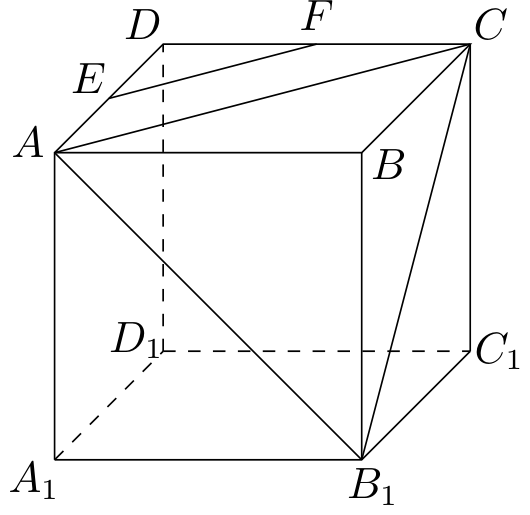
\includegraphics[width=5.3cm]{GaoKao/images/2011/fujian_liberal/q15_fig1.png}
\end{center}
\end{center}

        \item 商家通常依据“乐观系数准则”确定商品销售价格，即根据商品的最低销售限价 \(a\)，最高销售限价 \(b\)（\(b > a\)）以及实数 \(x\)（\(0 < x < 1\)）确定实际销售价格 \( c = a + x (b - a) \). 这里，\(x\) 被称为乐观系数. 经验表明，最佳乐观系数 \(x\) 恰好使得 \( (c - a) \) 是 \( (b - c) \) 和 \( (b - a) \) 的等比中项. 据此可得，最佳乐观系数 \(x\) 的值等于\rule[-0.3ex]{3em}{0.4pt}.

    \end{enumerate}

\end{description}

\begin{description}

    \item[三、解答题]

    \begin{enumerate}[leftmargin=5pt]

      \addtocounter{enumi}{+16}

        \item 已知等差数列 \(\{a_{n}\}\) 中，\(a_{1} = 1\)，\(a_{3} = -3\).

\begin{enumerate}
\item 求数列 \( \{a_{n}\} \) 的通项公式；
\item 若数列 \( \{a_{n}\} \) 的前 \(k\) 项和 \( S_{k} = -35 \)，求 \(k\) 的值.
\end{enumerate}

        \item 如图，直线 \(l\)：\(y = x + b\) 与抛物线 \(C\)：\(x^2 = 4y\) 相切于点 \(A\).

\begin{enumerate}
\item 求实数 \(b\) 的值；
\item 求以点 \(A\) 为圆心，且与抛物线 \(C\) 的准线相切的圆的方程.
\end{enumerate}

\begin{center}
\begin{center}
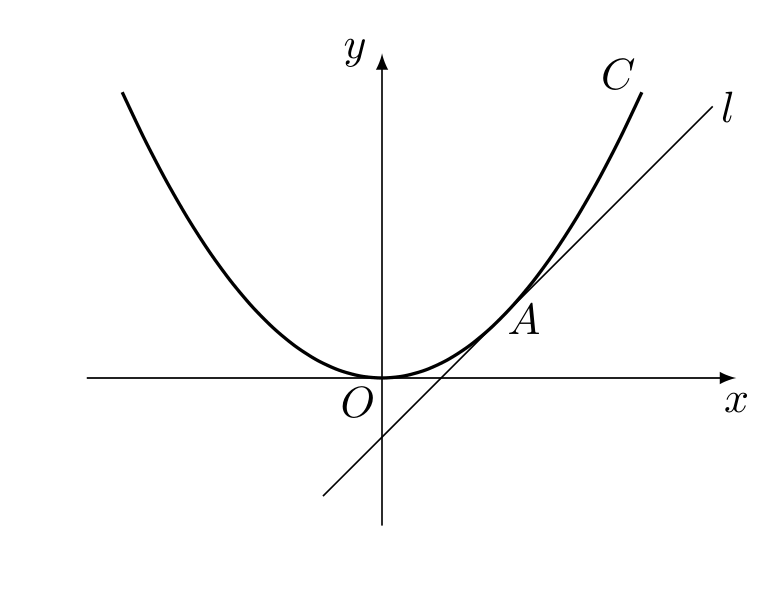
\includegraphics[width=9.0cm]{GaoKao/images/2011/fujian_liberal/q18_fig1.png}
\end{center}
\end{center}

        \item 某日用品按行业质量标准分成五个等级. 等级系数 \(X\) 依次为 \(1\)，\(2\)，\(3\)，\(4\)，\(5\). 现从一批该日用品中随机抽取 20 件，对其等级系数进行统计分析，得到频率分布表如下：

\begin{center}
\begin{tabular}{c|ccccc}
\(X\) & \(1\) & \(2\) & \(3\) & \(4\) & \(5\) \\
\hline
\(f\) & \(a\) & \(0.2\) & \(0.45\) & \(b\) & \(c\)
\end{tabular}
\end{center}

\begin{enumerate}
\item 若所抽取的 20 件日用品中，等级系数为 4 的恰有 3 件，等级系数为 5 的恰有 2 件，求 \(a\)，\(b\)，\(c\) 的值；
\item 在上问的条件下，将等级系数为 4 的 3 件日用品记为 \(x_{1}\)，\(x_{2}\)，\(x_{3}\)，等级系数为 5 的 2 件日用品记为 \(y_{1}\)，\(y_{2}\). 现从 \(x_{1}\)，\(x_{2}\)，\(x_{3}\)，\(y_{1}\)，\(y_{2}\) 这 5 件日用品中任取两件（假定每件日用品被取出的可能性相同），写出所有可能的结果，并求这两件日用品的等级系数恰好相等的概率.
\end{enumerate}

        \item 如图，四棱锥 \(P - ABCD\) 中，\(PA \perp\) 底面 \(ABCD\)，\(AB \perp AD\)，点 \(E\) 在线段 \(AD\) 上，且 \(CE \parallel AB\).

\begin{enumerate}
\item 求证：\( CE \perp \) 平面 \(PAD\)；
\item 若 \(PA = AB = 1\)，\(AD = 3\)，\(CD = \sqrt{2}\)，\(\angle CDA = 45^{\circ}\)，求四棱锥 \(P - ABCD\) 的体积.
\end{enumerate}

\begin{center}
\begin{center}
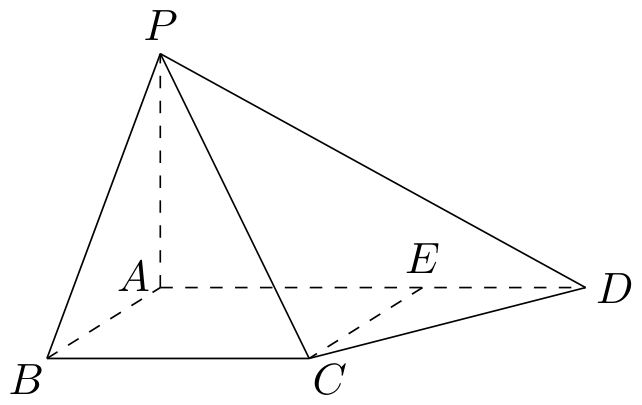
\includegraphics[width=6.3cm]{GaoKao/images/2011/fujian_liberal/q20_fig1.png}
\end{center}
\end{center}

        \item 设函数 \( f(\theta) = \sqrt{3}\sin \theta + \cos \theta \)，其中，角 \( \theta \) 的顶点与坐标原点重合，始边与 \( x \) 轴非负半轴重合，终边经过点 \( P(x, y) \)，且 \( 0 \leqslant \theta \leqslant \pi \).

\begin{enumerate}
\item 若点 \(P\) 的坐标为 \(\left(\frac{1}{2}, \frac{\sqrt{3}}{2}\right)\)，求 \(f(\theta)\) 的值；
\item 若点 \(P(x, y)\) 为平面区域 \(\Omega\)：\(\begin{cases}
x + y \geqslant 1,\\
x \leqslant 1,\\
y \leqslant 1
\end{cases}\) 上的一个动点，试确定角 \(\theta\) 的取值范围，并求函数 \(f(\theta)\) 的最小值和最大值.
\end{enumerate}

        \item 已知 \(a\)，\(b\) 为常数，且 \(a \neq 0\). 函数 \(f(x) = -ax + b + ax \ln x\)，\(f({\mathrm{e}}) = 2\)（\({\mathrm{e}} = 2.71828 \cdots\) 是自然对数的底数）.

\begin{enumerate}
\item 求实数 \(b\) 的值；
\item 求函数 \( f(x) \) 的单调区间；
\item 当 \(a = 1\) 时，是否同时存在实数 \(m\) 和 \(M\)（\(m < M\)），使得对每一个 \(t \in [m, M]\)，直线 \(y = t\) 与曲线 \(y = f(x)\)（\(x \in \left[ \frac{1}{2}, {\mathrm{e}} \right]\)）都有公共点？若存在，求出最小的实数 \(m\) 和最大的实数 \(M\)；若不存在，说明理由.
\end{enumerate}

    \end{enumerate}

\end{description}


\subsection{2011年广东卷（理）}\label{gk:2011年广东卷（理）}

\begin{description}

    \item[一、选择题]

    \begin{enumerate}[leftmargin=5pt]

        \item 设复数 \(z\) 满足 \((1 + \i)z = 2\)，其中 \(\i\) 为虚数单位，则 \(z =\)（\quad）

        {\centering\begin{tabular*}{\linewidth}{@{}@{\extracolsep{\fill}}llll@{}}
          \text{A. }\(1 + \i\)  &  \text{B. }\(1 - \i\)  &  \text{C. }\(2 + 2\i\)  &  \text{D. }\(2 - 2\i\)
        \end{tabular*}\par}

        \item 已知集合 \(A = \{(x, y) | x, y\) 为实数，且 \(x^2 + y^2 = 1\}\)，\(B = \{(x, y) | x, y\) 为实数，且 \(y = x\}\)，则 \(A \cap B\) 的元素个数为（\quad）

        {\centering\begin{tabular*}{\linewidth}{@{}@{\extracolsep{\fill}}llll@{}}
          \text{A. }\(0\)  &  \text{B. }\(1\)  &  \text{C. }\(2\)  &  \text{D. }\(3\)
        \end{tabular*}\par}

        \item 若非零向量 \(a\)，\(b\)，\(c\) 满足 \(a \parallel b\) 且 \(a \perp c\)，则 \(c \cdot (a + 2b) =\)（\quad）

        {\centering\begin{tabular*}{\linewidth}{@{}@{\extracolsep{\fill}}llll@{}}
          \text{A. }\(4\)  &  \text{B. }\(3\)  &  \text{C. }\(2\)  &  \text{D. }\(0\)
        \end{tabular*}\par}

        \item 设函数 \( f(x) \) 和 \( g(x) \) 分别是 \( \mathbb{R} \) 上的偶函数和奇函数，则下列结论恒成立的是（\quad）

        {\centering\begin{tabular*}{\linewidth}{@{}@{\extracolsep{\fill}}llll@{}}
          \text{A. }\(f(x) + |g(x)|\) 是偶函数  &  \text{B. }\(f(x) - |g(x)|\) 是奇函数  &  \text{C. }\(|f(x)| + g(x)\) 是偶函数  &  \text{D. }\( |f(x)| - g(x) \) 是奇函数
        \end{tabular*}\par}

        \item 已知平面直角坐标系 \(xOy\) 上的区域 \(D\) 由不等式组 \(\begin{cases}
0 \leqslant x \leqslant \sqrt{2},\\
y \leqslant 2,\\
x \leqslant \sqrt{2} y
\end{cases}\) 给定. 若 \(M(x,y)\) 为 \(D\) 上的动点，点 \(A\) 的坐标为 \((\sqrt{2},1)\)，则 \(z = \overrightarrow{OM} \cdot \overrightarrow{OA}\) 的最大值为（\quad）

        {\centering\begin{tabular*}{\linewidth}{@{}@{\extracolsep{\fill}}llll@{}}
          \text{A. }\(4\sqrt{2}\)  &  \text{B. }\(3\sqrt{2}\)  &  \text{C. }4  &  \text{D. }3
        \end{tabular*}\par}

        \item 甲，乙两队进行排球决赛. 现在的情形是甲队只要再赢一局就获冠军，乙队需要再赢两局才能得冠军. 若两队胜每局的概率相同，则甲队获得冠军的概率为（\quad）

        {\centering\begin{tabular*}{\linewidth}{@{}@{\extracolsep{\fill}}llll@{}}
          \text{A. }\(\frac{1}{2}\)  &  \text{B. }\( \frac{3}{5} \)  &  \text{C. }\( \frac{2}{3} \)  &  \text{D. }\( \frac{3}{4} \)
        \end{tabular*}\par}

        \item 如图，某几何体的正视图（主视图）是平行四边形，侧视图（左视图）和俯视图都是矩形，则该几何体的体积为（\quad）

\begin{center}
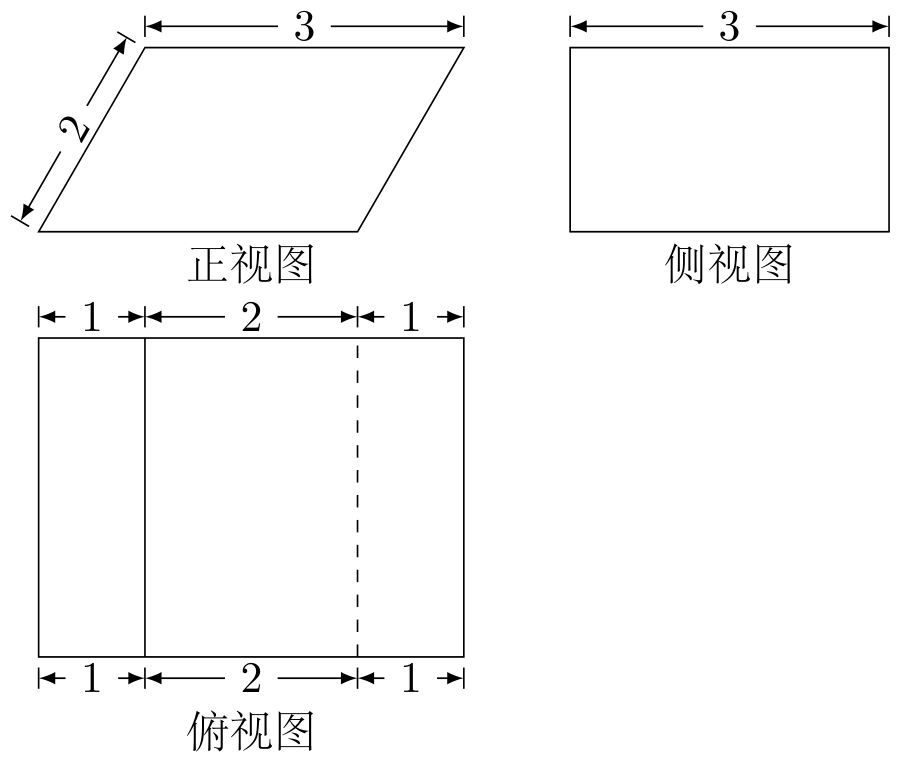
\includegraphics[width=8.8cm]{GaoKao/images/2011/guangdong_science/q7_fig1.png}
\end{center}

        {\centering\begin{tabular*}{\linewidth}{@{}@{\extracolsep{\fill}}llll@{}}
          \text{A. }\(6\sqrt{3}\)  &  \text{B. }\(9\sqrt{3}\)  &  \text{C. }\(12\sqrt{3}\)  &  \text{D. }\(18\sqrt{3}\)
        \end{tabular*}\par}

        \item 设 \(S\) 是整数集 \(\mathbb{Z}\) 的非空子集，如果对于 \(\forall a,b\in S\)，有 \(ab \in S\)，则称 \(S\) 关于数的乘法是封闭的. 若 \(T\)，\(V\) 是 \(\mathbb{Z}\) 的两个不相交的非空子集，\(T \cup V = \mathbb{Z}\). 且对于 \(\forall a,b,c\in T\)，有 \(abc \in T\)，\(\forall x,y,z\in V\)，有 \(xyz \in V\). 则下列结论恒成立的是（\quad）

        {\centering\begin{tabular*}{\linewidth}{@{}@{\extracolsep{\fill}}llll@{}}
          \text{A. }\(T\)，\( V\) 中至少有一个关于乘法是封闭的  &  \text{B. }\(T\)，\(V\) 中至多有一个关于乘法是封闭的  &  \text{C. }\(T\)，\(V\) 中有且只有一个关于乘法是封闭的  &  \text{D. }\(T\)，\(V\) 中每一个关于乘法都是封闭的
        \end{tabular*}\par}

    \end{enumerate}

\end{description}

\begin{description}

    \item[二、填空题]

    \begin{enumerate}[leftmargin=5pt]

      \addtocounter{enumi}{+8}

        \item 不等式 \(|x + 1| - |x - 3| \geqslant 0\) 的解集是\rule[-0.3ex]{3em}{0.4pt}.

        \item \(x\left(x - \frac{2}{x}\right)^7\) 的展开式中，\(x^4\) 的系数是\rule[-0.3ex]{3em}{0.4pt}. （用数字作答）

        \item 等差数列 \(\{a_{n}\}\) 前9项的和等于前4项的和. 若 \(a_{1} = 1\)，\(a_{k} + a_{4} = 0\)，则 \(k = \)\rule[-0.3ex]{3em}{0.4pt}.

        \item 函数 \( f(x) = x^3 - 3x^2 + 1 \) 在 \( x =\rule[-0.3ex]{3em}{0.4pt} \) 处取得极小值.

        \item 某数学老师身高 \(176\mathrm{~cm}\)，他爷爷，父亲和儿子的身高分别是 \(173\mathrm{~cm}\)，\(170\mathrm{~cm}\) 和 \(182\mathrm{~cm}\). 因儿子的身高与父亲的身高有关，该老师用线性回归分析的方法预测他孙子的身高为\rule[-0.3ex]{3em}{0.4pt}\(\mathrm{cm}\).

    \end{enumerate}

\end{description}

\begin{description}

    \item[三、选考题]

    \begin{enumerate}[leftmargin=5pt]

      \addtocounter{enumi}{+13}

        \item \textbf{【选修4-4：坐标系与参数方程】}

已知两曲线参数方程分别为 \(\begin{cases}
x = \sqrt{5} \cos \theta,\\
y = \sin \theta,
\end{cases}\)（\(0 \leqslant \theta < \pi\)）和 \(\begin{cases}
x = \frac{5}{4} t^2,\\
y = t,
\end{cases}\)（\(t \in \mathbb{R}\)），它们的交点坐标为\rule[-0.3ex]{3em}{0.4pt}.

        \item \textbf{【选修4-1：几何证明选讲】}

如图，过圆 \(O\) 外一点 \(P\) 分别作圆的切线和割线，交于 \(A\)，\(B\)，且 \(PB = 7\)，\(C\) 是圆上一点，使得 \(BC = 5\)，\(\angle BAC = \angle APB\)，则 \(AB =\rule[-0.3ex]{3em}{0.4pt}\).

\begin{center}
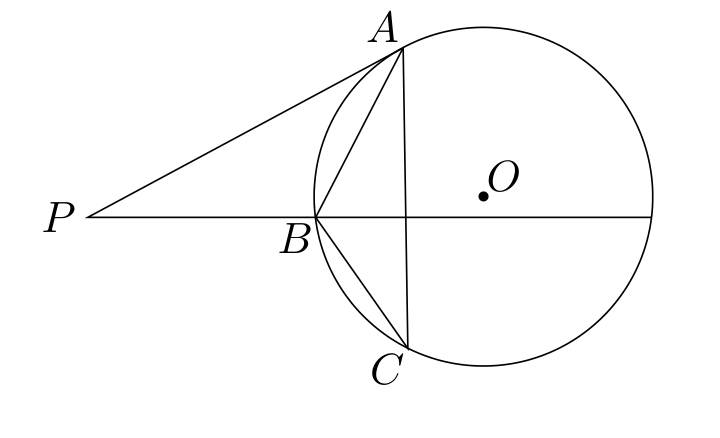
\includegraphics[width=6.5cm]{GaoKao/images/2011/guangdong_science/q15_fig1.png}
\end{center}

    \end{enumerate}

\end{description}

\begin{description}

    \item[四、解答题]

    \begin{enumerate}[leftmargin=5pt]

      \addtocounter{enumi}{+15}

        \item \begin{enumerate}
\item 已知函数 \(f(x) = 2\sin \left(\frac{1}{3} x - \frac{\pi}{6}\right)\)，\(x \in \mathbb{R}\). 求 \( f\left(\frac{5\pi}{4}\right) \) 的值.
\item 设 \(\alpha\)，\(\beta \in \left[0, \frac{\pi}{2}\right]\)，\(f\left(3\alpha + \frac{\pi}{2}\right) = \frac{10}{13}\)，\(f(3\beta + 2\pi) = \frac{6}{5}\)，求 \(\cos (\alpha + \beta)\) 的值.
\end{enumerate}

        \item 为了解甲，乙两厂的产品质量，采用分层抽样的方法从甲，乙两厂生产的产品中分别抽取 14 件和 5 件，测量产品中微量元素 \(x\)，\(y\) 的含量（单位：毫克）. 下表是乙厂的 5 件产品的测量数据：

\begin{center}
\begin{tabular}{|c|c|c|c|c|c|}
\hline
编号 & 1 & 2 & 3 & 4 & 5 \\
\hline
\(x\) & 169 & 178 & 166 & 175 & 180 \\
\hline
\(y\) & 75 & 80 & 77 & 70 & 81 \\
\hline
\end{tabular}
\end{center}

\begin{enumerate}
\item 已知甲厂生产的产品共有 98 件，求乙厂生产的产品数量.
\item 当产品中的微量元素 \(x\)，\(y\) 满足 \(x \geqslant 175\) 且 \(y \geqslant 75\) 时，该产品为优等品. 用上述样本数据估计乙厂生产的优等品的数量.
\item 从乙厂抽出的上述 5 件产品中，随机抽取 2 件，求抽取的 2 件产品中优等品数 \(\xi\) 的分布列及其均值（即数学期望）.
\end{enumerate}

        \item 如图，在锥体 \(P - ABCD\) 中，\(ABCD\) 是边长为 1 的菱形，且 \(\angle DAB = 60^{\circ}\)，\(PA = PD = \sqrt{2}\)，\(PB = 2\)，\(E\)，\(F\) 分别是 \(BC\)，\(PC\) 的中点.

\begin{enumerate}
\item 证明：\(AD \perp\) 平面 \(DEF\).
\item 求二面角 \(P-AD-B\) 的余弦值.
\end{enumerate}

\begin{center}
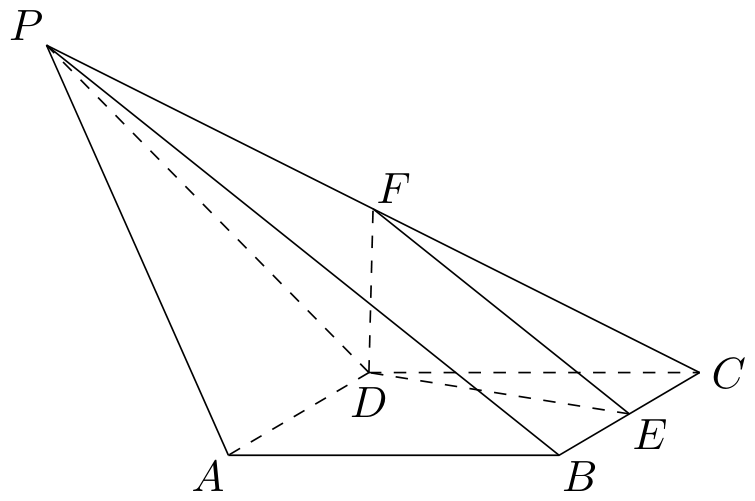
\includegraphics[width=9.4cm]{GaoKao/images/2011/guangdong_science/q18_fig1.png}
\end{center}

        \item \begin{enumerate}
\item 设圆 \(C\) 与两圆 \((x + \sqrt{5})^2 + y^2 = 4\)，\((x - \sqrt{5})^2 + y^2 = 4\) 中的一个内切，另一个外切. 求 \(C\) 的圆心轨迹 \(L\) 的方程.
\item 已知点 \(M\left(\frac{3\sqrt{5}}{5}, \frac{4\sqrt{5}}{5}\right)\)，\(F(\sqrt{5}, 0)\)，且 \(P\) 为 \(L\) 上动点，求 \(\|MP\| - \|FP\|\) 的最大值及此时点 \(P\) 的坐标.
\end{enumerate}

        \item \begin{enumerate}
\item 设 \(b > 0\)，数列 \(\{a_{n}\}\) 满足 \(a_{1} = b\)，\(a_{n} = \frac{nba_{n-1}}{a_{n-1} + 2n - 2}\)（\(n \geqslant 2\)）. 求数列 \(\{a_{n}\}\) 的通项公式.
\item 证明：对于一切正整数 \(n\)，\(a_{n} \leqslant \frac{b^{n+1}}{2^{n+1}} + 1\).
\end{enumerate}

        \item \begin{enumerate}
\item 在平面直角坐标系 \(xOy\) 上，给定抛物线 \(L: y = \frac{1}{4} x^2\). 实数 \(p\)，\(q\) 满足 \(p^2 - 4q \geqslant 0\)，\(x_1\)，\(x_2\) 是方程 \(x^2 - px + q = 0\) 的两根. 记 \(\varphi(p, q) = \max \{|x_1|, |x_2|\}\). 过点 \(A\left(p_0, \frac{1}{4} p_0^2\right)\)（\(p_0 \neq 0\)）作 \(L\) 的切线交 \(y\) 轴于点 \(B\). 证明：对线段 \(AB\) 上的任一点 \(Q(p, q)\)，有 \(\varphi(p, q) = \frac{|p_0|}{2}\).
\item 设 \(M(a, b)\) 是定点，其中 \(a\)，\(b\) 满足 \(a^2 - 4b > 0\)，\(a \neq 0\). 过点 \(M(a, b)\) 作 \(L\) 的两条切线 \(l_1\)，\(l_2\)，切点分别为 \(E\left(p_1, \frac{1}{4} p_1^2\right)\)，\(E'\left(p_2, \frac{1}{4} p_2^2\right)\)，\(l_1\)，\(l_2\) 与 \(y\) 分别交于 \(F\)，\(F'\). 线段 \(EF\) 上异于两端点的点集记为 \(X\). 证明：\(M(a, b) \in X \Leftrightarrow |p_1| > |p_2| \Leftrightarrow \varphi(a, b) = \frac{|p_1|}{2}\).
\item 设 \(D = \left\{(x, y) \mid y \leqslant x - 1, y \geqslant \frac{1}{4} (x + 1)^2 - \frac{5}{4}\right\}\). 当点 \((p, q)\) 取遍 D 时，求 \(\varphi(p, q)\) 的最小值（记为 \(\varphi_{\min}\)）和最大值（记为 \(\varphi_{\max}\)）.
\end{enumerate}

    \end{enumerate}

\end{description}


\subsection{2011年广东卷（文）}\label{gk:2011年广东卷（文）}

\begin{description}

    \item[一、选择题]

    \begin{enumerate}[leftmargin=5pt]

        \item 设复数 \(z\) 满足 \(\i z = 1\)，其中 \(\i\) 为虚数单位，则 \(z =\)（\quad）

        {\centering\begin{tabular*}{\linewidth}{@{}@{\extracolsep{\fill}}llll@{}}
          \text{A. }\(-\i\)  &  \text{B. }\(\i\)  &  \text{C. }\(-1\)  &  \text{D. }\(1\)
        \end{tabular*}\par}

        \item 已知集合 \(A = \{(x, y) | x, y\) 为实数，且 \(x^2 + y^2 = 1\}\)，\(B = \{(x, y) | x, y\) 为实数，且 \(x + y = 1\}\)，则 \(A \cap B\) 的元素个数为（\quad）

        {\centering\begin{tabular*}{\linewidth}{@{}@{\extracolsep{\fill}}llll@{}}
          \text{A. }\(4\)  &  \text{B. }\(3\)  &  \text{C. }\(2\)  &  \text{D. }\(1\)
        \end{tabular*}\par}

        \item 已知向量 \(\bm{a} = (1, 2)\)，\(\bm{b} = (1, 0)\)，\(\bm{c} = (3, 4)\). 若 \(\lambda\) 为实数，\((\bm{a} + \lambda \bm{b}) \parallel \bm{c}\)，则 \(\lambda = \)（\quad）

        {\centering\begin{tabular*}{\linewidth}{@{}@{\extracolsep{\fill}}llll@{}}
          \text{A. }\( \frac{1}{4} \)  &  \text{B. }\( \frac{1}{2} \)  &  \text{C. }\(1\)  &  \text{D. }\(2\)
        \end{tabular*}\par}

        \item 函数 \( f(x) = \frac{1}{1 - x} + \lg (1 + x) \) 的定义域是（\quad）

        {\centering\begin{tabular*}{\linewidth}{@{}@{\extracolsep{\fill}}llll@{}}
          \text{A. }\((-\infty, -1)\)  &  \text{B. }\((1, +\infty)\)  &  \text{C. }\((-1,1)\cup (1, + \infty)\)  &  \text{D. }\((-\infty, +\infty)\)
        \end{tabular*}\par}

        \item 不等式 \(2x^{2} - x - 1 > 0\) 的解集是（\quad）

        {\centering\begin{tabular*}{\linewidth}{@{}@{\extracolsep{\fill}}llll@{}}
          \text{A. }\( \left(-\frac{1}{2},1\right) \)  &  \text{B. }\((1, + \infty)\)  &  \text{C. }\((-\infty, 1) \cup (2, +\infty)\)  &  \text{D. }\(\left(-\infty, -\frac{1}{2}\right) \cup (1, +\infty)\)
        \end{tabular*}\par}

        \item 已知平面直角坐标系 \(xOy\) 上的区域 \(D\) 由不等式组 \(\begin{cases}
0 \leqslant x \leqslant \sqrt{2},\\
y \leqslant 2,\\
x \leqslant \sqrt{2}y
\end{cases}\) 给定。若 \(M(x, y)\) 为 \(D\) 上的动点，点 \(A\) 的坐标为 \((\sqrt{2}, 1)\)，则 \(z = \overrightarrow{OM} \cdot \overrightarrow{OA}\) 的最大值为（\quad）

        {\centering\begin{tabular*}{\linewidth}{@{}@{\extracolsep{\fill}}llll@{}}
          \text{A. }\(3\)  &  \text{B. }\(4\)  &  \text{C. }\( 3\sqrt{2} \)  &  \text{D. }\(4\sqrt{2}\)
        \end{tabular*}\par}

        \item 正五棱柱中，不同在任何侧面且不同在任何底面的两顶点的连线称为它的对角线，那么一个正五棱柱对角线的条数共有（\quad）

        {\centering\begin{tabular*}{\linewidth}{@{}@{\extracolsep{\fill}}llll@{}}
          \text{A. }\(20\)  &  \text{B. }\(15\)  &  \text{C. }\(12\)  &  \text{D. }\(10\)
        \end{tabular*}\par}

        \item 设圆 \(C\) 与圆 \(x^{2}+(y-3)^{2}=1\) 外切，且与直线 \(y=0\) 相切，则 \(C\) 的圆心轨迹为（\quad）

        {\centering\begin{tabular*}{\linewidth}{@{}@{\extracolsep{\fill}}llll@{}}
          \text{A. }抛物线  &  \text{B. }双曲线  &  \text{C. }椭圆  &  \text{D. }圆
        \end{tabular*}\par}

        \item 如图，某几何体的正视图（主视图）、侧视图（左视图）和俯视图分别是等边三角形、等腰三角形和菱形，则该几何体的体积为（\quad）

\begin{center}
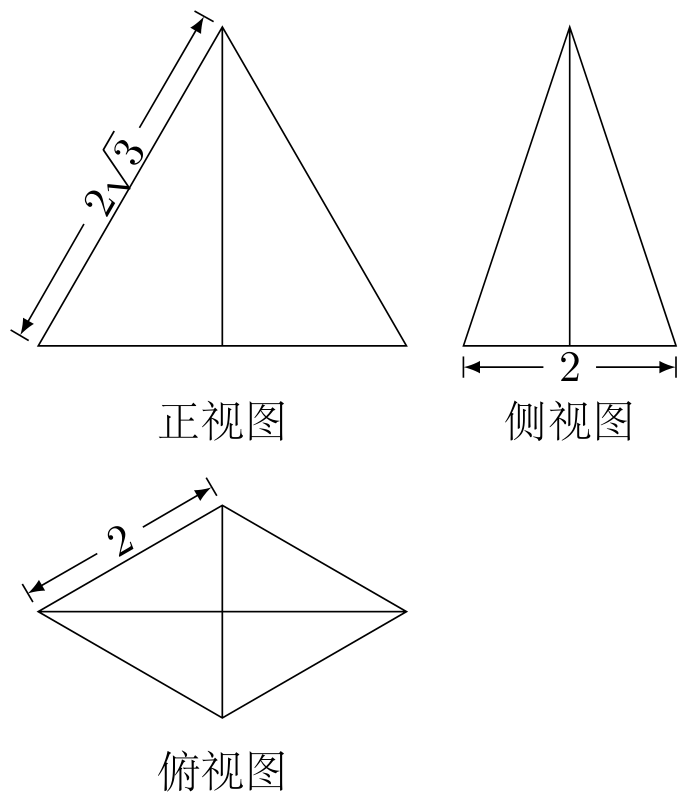
\includegraphics[width=6.8cm]{GaoKao/images/2011/guangdong_liberal/q9_fig1.png}
\end{center}

        {\centering\begin{tabular*}{\linewidth}{@{}@{\extracolsep{\fill}}llll@{}}
          \text{A. }\(4\sqrt{3}\)  &  \text{B. }\(4\)  &  \text{C. }\(2 \sqrt{3}\)  &  \text{D. }\(2\)
        \end{tabular*}\par}

        \item 设 \(f(x)\)，\(g(x)\)，\(h(x)\) 是 \(\mathbb{R}\) 上的任意实值函数. 如下定义两个函数 \((f \circ g)(x)\) 和 \((f \bullet g)(x)\)：对任意 \(x \in \mathbb{R}\)，\((f \circ g)(x) = f(g(x))\)；\((f \bullet g)(x) = f(x)g(x)\)，则下列等式恒成立的是（\quad）

        {\centering\begin{tabular*}{\linewidth}{@{}@{\extracolsep{\fill}}llll@{}}
          \text{A. }\(\big((f\circ g)\bullet h\big)(x) = \big((f\bullet h)\circ (g\bullet h)\big)(x)\)  &  \text{B. }\(\big((f\bullet g)\circ h\big)(x) = \big((f\circ h)\bullet (g\circ h)\big)(x)\)  &  \text{C. }\(\big((f\circ g)\circ h\big)(x) = \big((f\circ h)\circ (g\circ h)\big)(x)\)  &  \text{D. }\(\big((f\bullet g)\bullet h\big)(x) = \big((f\bullet h)\bullet (g\bullet h)\big)(x)\)
        \end{tabular*}\par}

    \end{enumerate}

\end{description}

\begin{description}

    \item[二、填空题]

    \begin{enumerate}[leftmargin=5pt]

      \addtocounter{enumi}{+10}

        \item 已知 \(\{a_{n}\}\) 是递增的等比数列，\(a_{2} = 2\)，\(a_{4} - a_{3} = 4\). 则此数列的公比 \(q = \)\rule[-0.3ex]{3em}{0.4pt}.

        \item 设函数 \( f(x) = x^{3}\cos x + 1 \). 若 \( f(a) = 11 \)，则 \( f(-a) = \)\rule[-0.3ex]{3em}{0.4pt}.

        \item 为了解篮球爱好者小李的投篮命中率与打篮球时间之间的关系. 下表记录了小李某月 \(1\) 号到 \(5\) 号每天打篮球时间 \(x\)（单位：小时）与当天投篮命中率 \(y\) 之间的关系：

\begin{center}
\begin{tabular}{c|ccccc}
时间 \(x\) & \(1\) & \(2\) & \(3\) & \(4\) & \(5\) \\
\hline
命中率 \(y\) & \(0.4\) & \(0.5\) & \(0.6\) & \(0.6\) & \(0.4\)
\end{tabular}
\end{center}

小李这 5 天的平均投篮命中率为\rule[-0.3ex]{3em}{0.4pt}；用线性回归分析的方法，预测小李该月 6 号打 6 小时篮球的投篮命中率为\rule[-0.3ex]{3em}{0.4pt}.

    \end{enumerate}

\end{description}

\begin{description}

    \item[三、选考题]

    \begin{enumerate}[leftmargin=5pt]

      \addtocounter{enumi}{+13}

        \item \textbf{【选修4-4：坐标系与参数方程】}

已知两曲线参数方程分别为 \(\begin{cases}
x = \sqrt{5} \cos \theta,\\
y = \sin \theta,
\end{cases}\) （\(0 \leqslant \theta < \pi\)） 和 \(\begin{cases}
x = \frac{5}{4} t^2,\\
y = t,
\end{cases}\) （\(t \in \mathbb{R}\)） ，它们的交点坐标为\rule[-0.3ex]{3em}{0.4pt}.

        \item 如图，在梯形 \(ABCD\) 中，\(AB \parallel CD\)，\(AB = 4\)，\(CD = 2\)，\(E\)，\(F\) 分别为 \(AD\)，\(BC\) 上的点，且 \(EF = 3\)，\(EF \parallel AB\)，则梯形 \(ABFE\) 与梯形 \(EFCD\) 的面积比为\rule[-0.3ex]{3em}{0.4pt}.

\begin{center}
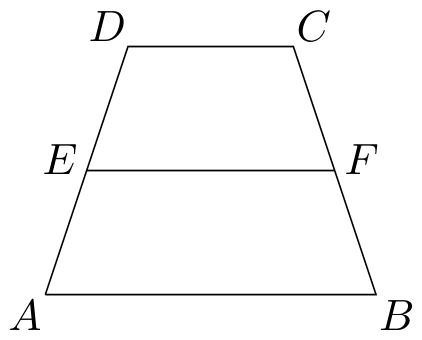
\includegraphics[width=5.1cm]{GaoKao/images/2011/guangdong_liberal/q15_fig1.png}
\end{center}

    \end{enumerate}

\end{description}

\begin{description}

    \item[四、解答题]

    \begin{enumerate}[leftmargin=5pt]

      \addtocounter{enumi}{+15}

        \item 已知函数 \(f(x) = 2\sin \left(\frac{1}{3} x - \frac{\pi}{6}\right)\)，\(x \in \mathbb{R}\).
\begin{enumerate}
\item 求 \( f(0) \) 的值；
\item 设 \(\alpha\)，\(\beta \in \left[0, \frac{\pi}{2}\right]\)，\(f\left(3\alpha + \frac{\pi}{2}\right) = \frac{10}{13}\)，\(f(3\beta + 2\pi) = \frac{6}{5}\)，求 \(\sin (\alpha + \beta)\) 的值.
\end{enumerate}

        \item 在某次测验中，有 6 位同学的平均成绩为 75 分. 用 \( x_{n} \) 表示编号为 \(n\) （\(n = 1, 2, \cdots, 6\)）的同学所得成绩，且前 5 位同学的成绩如下：

\begin{center}
\begin{tabular}{c|ccccc}
编号 \(n\) & \(1\) & \(2\) & \(3\) & \(4\) & \(5\) \\
\hline
成绩 \(x_{n}\) & \(70\) & \(76\) & \(72\) & \(70\) & \(72\)
\end{tabular}
\end{center}

\begin{enumerate}
\item 求第 6 位同学的成绩 \(x_6\)，及这 6 位同学成绩的标准差 \(s\)；
\item 从前 5 位同学中，随机地选 2 位同学，求恰有 1 位同学成绩在区间 \((68, 75)\) 中的概率.
\end{enumerate}

        \item 如图所示的几何体是将高为 2、底面半径为 1 的直圆柱沿过轴的平面切开后，将其中一半沿切面向右水平平移后得到的. \(A\)，\(A'\)，\(B\)，\(B'\) 分别为 \(\overset{\frown}{CD}\)，\(\overset{\frown}{C'D'}\)，\(\overset{\frown}{DE}\)，\(\overset{\frown}{D'E'}\) 的中点，\(O_1\)，\(O_1'\)，\(O_2\)，\(O_2'\) 分别为 \(CD\)，\(C'D'\)，\(DE\)，\(D'E'\) 的中点.

\begin{enumerate}
\item 证明： \(O_{1}^{\prime}\)，\(A^{\prime}\)，\(O_{2}\)，\(B\) 四点共面；
\item 设 G 为 \( A^{\prime}A \) 中点，延长 \( A^{\prime}O_{1}^{\prime} \) 到 \( H^{\prime} \)，使得 \( O_{1}^{\prime}H^{\prime}=A^{\prime}O_{1}^{\prime} \)，证明： \( BO_{2}^{\prime}\perp \) 平面 \( H^{\prime}B^{\prime}G \).
\end{enumerate}

\begin{center}
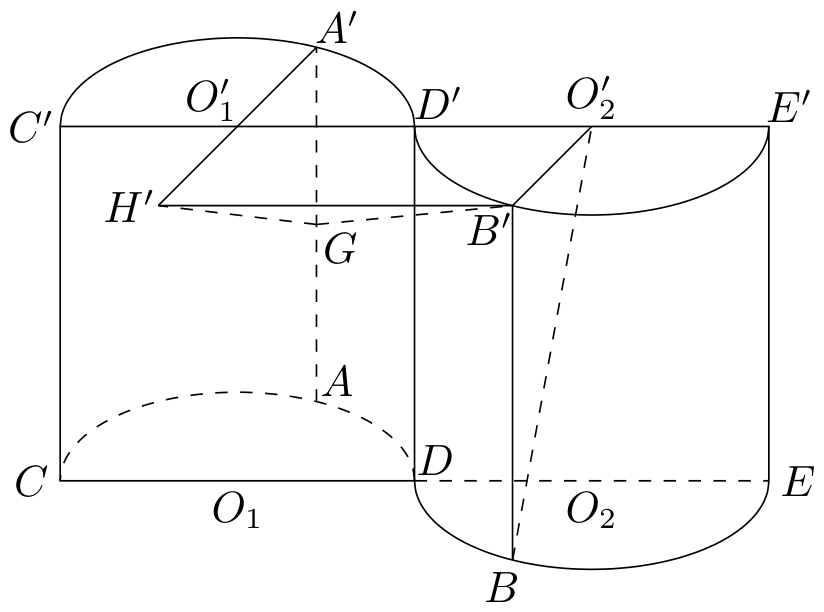
\includegraphics[width=7.8cm]{GaoKao/images/2011/guangdong_liberal/q18_fig1.png}
\end{center}

        \item 设 \(a > 0\)，讨论函数 \(f(x) = \ln x + a(1 - a)x^2 - 2(1 - a)x\) 的单调性.

        \item 设 \(b > 0\)，数列 \(\{a_{n}\}\) 满足 \(a_{1} = b\)，\(a_{n} = \frac{nba_{n - 1}}{a_{n - 1} + n - 1} \)（\(n \geqslant 2\)）.
\begin{enumerate}
\item 求数列 \( \{a_{n}\} \) 的通项公式；
\item 证明：对于一切正整数 \(n\)，\(2a_{n} \leqslant b^{n+1} + 1\).
\end{enumerate}

        \item 在平面直角坐标系 \(xOy\) 中，直线 \(l: x = -2\) 交 \(x\) 轴于点 \(A\). 设 \(P\) 是 \(l\) 上一点，\(M\) 是线段 \(OP\) 的垂直平分线上一点，且满足 \(\angle MPO = \angle AOP\).
\begin{enumerate}
\item 当点 \(P\) 在 \(l\) 上运动时，求点 \(M\) 的轨迹 \(E\) 的方程；
\item 已知 \(T(1,-1)\)，设 \(H\) 是 \(E\) 上动点，求 \( |HO| + |HT| \) 的最小值，并给出此时点 \(H\) 的坐标；
\item 过点 \(T(1, -1)\) 且不平行于 \(y\) 轴的直线 \(l_{1}\) 与轨迹 E 有且只有两个不同的交点，求直线 \(l_{1}\) 的斜率 \(k\) 的取值范围.
\end{enumerate}

    \end{enumerate}

\end{description}


\subsection{2011年湖北卷（理）}\label{gk:2011年湖北卷（理）}

\begin{description}

    \item[一、选择题]

    \begin{enumerate}[leftmargin=5pt]

        \item \(\i\) 为虚数单位，则 \( \left(\frac{1+\i}{1-\i}\right)^{2011}= \)（\quad）

        {\centering\begin{tabular*}{\linewidth}{@{}@{\extracolsep{\fill}}llll@{}}
          \text{A. }\(-\i\)  &  \text{B. }\(-1\)  &  \text{C. }\(\i\)  &  \text{D. }\(1\)
        \end{tabular*}\par}

        \item 已知 \(U = \{y \mid y = \log_2 x, x > 1\}\)，\(P = \left\{y \mid y = \frac{1}{x}, x > 2\right\}\)，则 \(\complement_U P =\)（\quad）

        {\centering\begin{tabular*}{\linewidth}{@{}@{\extracolsep{\fill}}llll@{}}
          \text{A. }\(\left[\frac{1}{2}, +\infty\right)\)  &  \text{B. }\(\left(0, \frac{1}{2}\right)\)  &  \text{C. }\((0, +\infty)\)  &  \text{D. }\((- \infty, 0) \cup \left[\frac{1}{2}, +\infty\right)\)
        \end{tabular*}\par}

        \item 已知函数 \(f(x) = \sqrt{3}\sin x - \cos x\)，\(x \in \mathbb{R}\). 若 \( f(x) \geqslant 1 \)，则 \( x \) 的取值范围为（\quad）

        {\centering\begin{tabular*}{\linewidth}{@{}@{\extracolsep{\fill}}llll@{}}
          \text{A. }\(\left\{x\mid k\pi +\frac{\pi}{3}\leqslant x\leqslant k\pi +\pi ,k\in \mathbb{Z}\right\}\)  &  \text{B. }\(\left\{x\mid 2k\pi +\frac{\pi}{3}\leqslant x\leqslant 2k\pi +\pi ,k\in \mathbb{Z}\right\}\)  &  \text{C. }\(\left\{x\mid k\pi +\frac{\pi}{6}\leqslant x\leqslant k\pi +\frac{5\pi}{6},k\in \mathbb{Z}\right\}\)  &  \text{D. }\(\left\{x\mid 2k\pi +\frac{\pi}{6}\leqslant x\leqslant 2k\pi +\frac{5\pi}{6},k\in \mathbb{Z}\right\}\)
        \end{tabular*}\par}

        \item 将两个顶点在抛物线 \( y^{2} = 2px  \) （\(p > 0\)）上，另一个顶点是此抛物线焦点的正三角形个数记为 \(n\)，则（\quad）

        {\centering\begin{tabular*}{\linewidth}{@{}@{\extracolsep{\fill}}llll@{}}
          \text{A. }\(n = 0\)  &  \text{B. }\(n = 1\)  &  \text{C. }\(n = 2\)  &  \text{D. }\(n \geqslant 3\)
        \end{tabular*}\par}

        \item 已知随机变量 \(\xi\) 服从正态分布 \(N(2, \sigma^2)\)，且 \(P(\xi < 4) = 0.8\)，则 \(P(0 < \xi < 2) =\)（\quad）

        {\centering\begin{tabular*}{\linewidth}{@{}@{\extracolsep{\fill}}llll@{}}
          \text{A. }\(0.6\)  &  \text{B. }\(0.4\)  &  \text{C. }\(0.3\)  &  \text{D. }\(0.2\)
        \end{tabular*}\par}

        \item 已知定义在 \(\mathbb{R}\) 上的奇函数 \(f(x)\) 和偶函数 \(g(x)\) 满足 \(f(x) + g(x) = a^x - a^{-x} + 2\)（\(a > 0\)，且 \(a \neq 1\)）. 若 \(g(2) = a\)，则 \(f(2) =\)（\quad）

        {\centering\begin{tabular*}{\linewidth}{@{}@{\extracolsep{\fill}}llll@{}}
          \text{A. }\(2\)  &  \text{B. }\(\frac{15}{4}\)  &  \text{C. }\(\frac{17}{4}\)  &  \text{D. }\(a^2\)
        \end{tabular*}\par}

        \item 如图，用 \(K\)，\(A_{1}\)，\(A_{2}\) 三类不同的元件连接成一个系统. 当 \(K\) 正常工作且 \(A_{1}\)，\(A_{2}\) 至少有一个正常工作时，系统正常工作. 已知 \(K\)，\(A_{1}\)，\(A_{2}\) 正常工作的概率依次为 0.9，0.8，0.8，则系统正常工作的概率为（\quad）

\begin{center}
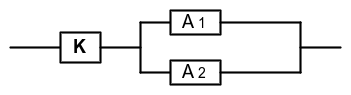
\includegraphics[width=9.3cm]{GaoKao/images/2011/hubei_science/q7_fig1.png}
\end{center}

        {\centering\begin{tabular*}{\linewidth}{@{}@{\extracolsep{\fill}}llll@{}}
          \text{A. }\(0.960\)  &  \text{B. }\(0.864\)  &  \text{C. }\(0.720\)  &  \text{D. }\(0.576\)
        \end{tabular*}\par}

        \item 已知向量 \(\bm{a} = (x + z, 3)\)，\(\bm{b} = (2, y - z)\)，且 \(\bm{a} \perp \bm{b}\). 若 \(x\)，\(y\) 满足不等式 \(|x| + |y| \leqslant 1\)，则 \(z\) 的取值范围为（\quad）

        {\centering\begin{tabular*}{\linewidth}{@{}@{\extracolsep{\fill}}llll@{}}
          \text{A. }\([-2, 2]\)  &  \text{B. }\([-2,3]\)  &  \text{C. }\([-3,2]\)  &  \text{D. }\([-3,3]\)
        \end{tabular*}\par}

        \item 若实数 \(a\)，\(b\) 满足 \(a \geqslant 0\)，\(b \geqslant 0\)，且 \(ab = 0\)，则称 \(a\) 与 \(b\) 互补. 记 \(\varphi(a, b) = \sqrt{a^2 + b^2} - a - b\)，那么 \(\varphi(a, b) = 0\) 是 \(a\) 与 \(b\) 互补的（\quad）

        {\centering\begin{tabular*}{\linewidth}{@{}@{\extracolsep{\fill}}llll@{}}
          \text{A. }必要而不充分条件  &  \text{B. }充分而不必要条件  &  \text{C. }充要条件  &  \text{D. }既不充分也不必要条件
        \end{tabular*}\par}

        \item 放射性元素由于不断有原子放射出微粒子而变成其他元素，其含量不断减少，这种现象称为衰变. 假设在放射性同位素铯 137 的衰变过程中，其含量 \(M\)（单位：太贝克）与时间 \(t\)（单位：年）满足函数关系：\(M(t) = M_0 2^{-t/30}\)，其中 \(M_0\) 为 \(t = 0\) 时铯 137 的含量. 已知 \(t = 30\) 时，铯 137 含量的变化率是 \(-10 \ln 2\)（太贝克/年），则 \(M(60) =\)（\quad）

        {\centering\begin{tabular*}{\linewidth}{@{}@{\extracolsep{\fill}}llll@{}}
          \text{A. }\(5\text{ 太贝克}\)  &  \text{B. }\(75 \ln 2\text{ 太贝克}\)  &  \text{C. }\(150 \ln 2\text{ 太贝克}\)  &  \text{D. }\(150\text{ 太贝克}\)
        \end{tabular*}\par}

    \end{enumerate}

\end{description}

\begin{description}

    \item[二、填空题]

    \begin{enumerate}[leftmargin=5pt]

      \addtocounter{enumi}{+10}

        \item \(\left(x - \frac{1}{3\sqrt{x}}\right)^{18}\) 的展开式中含 \(x^{15}\) 的项的系数为\rule[-0.3ex]{3em}{0.4pt}.（结果用数值表示）

        \item 在 \(30\) 瓶饮料中，有 \(3\) 瓶已过了保质期. 从这 \(30\) 瓶饮料中任取 \(2\) 瓶，则至少取到 \(1\) 瓶已过保质期饮料的概率为\rule[-0.3ex]{3em}{0.4pt}.（结果用最简分数表示）

        \item 《九章算术》“竹九节”问题：现有一根 \(9\) 节的竹子，自上而下各节的容积成等差数列，上面 \(4\) 节的容积共 \(3\text{ 升}\)，下面 \(3\) 节的容积共 \(4\text{ 升}\)，则第 \(5\) 节的容积为\rule[-0.3ex]{3em}{0.4pt}\(\text{升}\).

        \item 如图，直角坐标系 \(xOy\) 所在的平面为 \(\alpha\)，直角坐标系 \(x'Oy'\)（其中 \(y'\) 轴与 \(y\) 轴重合）所在的平面为 \(\beta\)，\(\angle xOx' = 45^\circ\).

\begin{enumerate}
\item 已知平面 \(\beta\) 内有一点 \(P'(2\sqrt{2}, 2)\)，则点 \(P'\) 在平面 \(\alpha\) 内的射影 \(P\) 的坐标为\rule[-0.3ex]{3em}{0.4pt}.
\item 已知平面 \(\beta\) 内的曲线 \(C'\) 的方程是 \(\left(x' - \sqrt{2}\right)^2 + 2y'^2 - 2 = 0\)，则曲线 \(C'\) 在平面 \(\alpha\) 内的射影 \(C\) 的方程是\rule[-0.3ex]{3em}{0.4pt}.
\end{enumerate}

\begin{center}
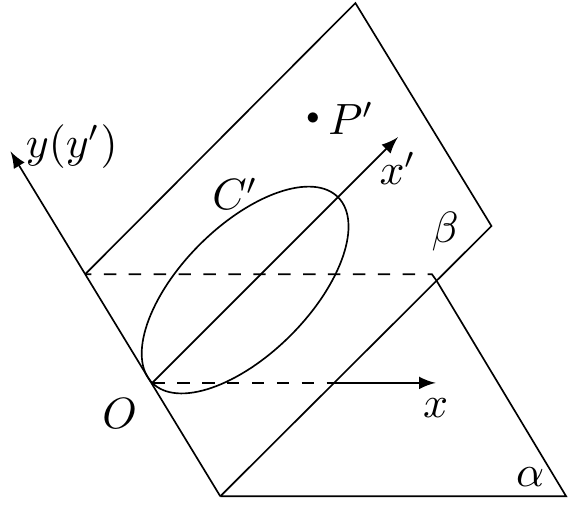
\includegraphics[width=5.4cm]{GaoKao/images/2011/hubei_science/q14_fig1.png}
\end{center}

        \item 给 \(n\) 个自上而下相连的正方形着黑色或白色，当 \(n \leqslant 4\) 时，在所有不同的着色方案中，黑色正方形互不相邻的着色方案如图所示：

由此推断，当 \(n = 6\) 时，黑色正方形互不相邻的着色方案共有\rule[-0.3ex]{3em}{0.4pt} 种，至少有两个黑色正方形相邻的着色方案共有\rule[-0.3ex]{3em}{0.4pt} 种. （结果用数值表示）
{\begin{center}
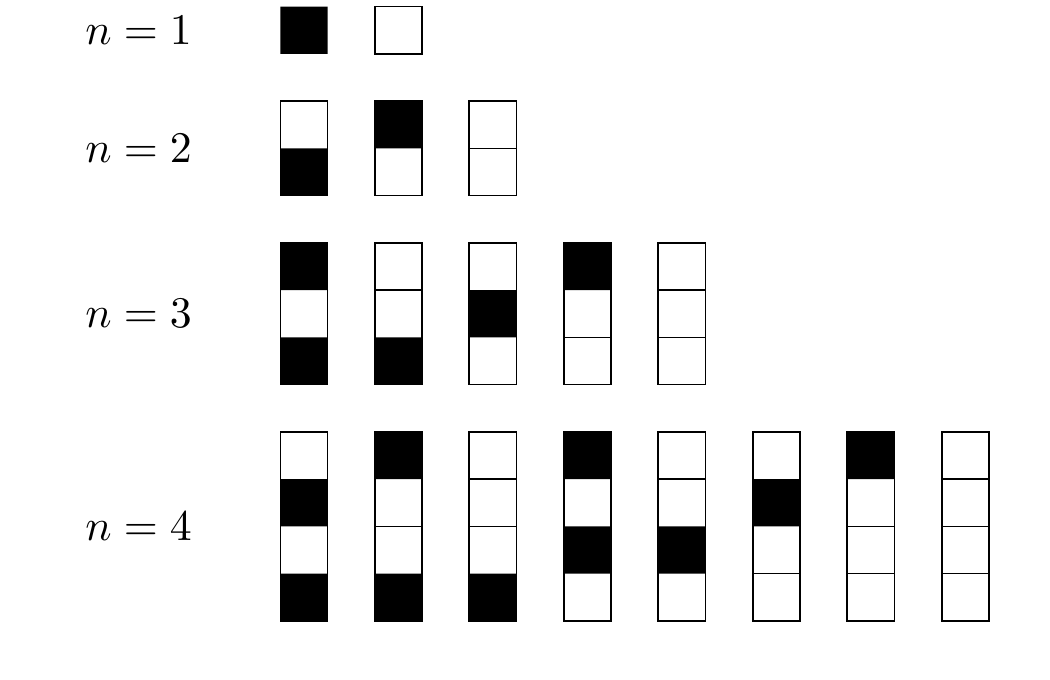
\includegraphics[width=9.0cm]{GaoKao/images/2011/hubei_science/q15_fig1.png}
\end{center}}

    \end{enumerate}

\end{description}

\begin{description}

    \item[三、解答题]

    \begin{enumerate}[leftmargin=5pt]

      \addtocounter{enumi}{+15}

        \item 设 \(\triangle ABC\) 的内角 \(A\)，\(B\)，\(C\) 所对的边分别为 \(a\)，\(b\)，\(c\). 已知 \(a = 1\)，\(b = 2\)，\(\cos C = \frac{1}{4}\).
\begin{enumerate}
\item 求 \( \triangle ABC \) 的周长；
\item 求 \( \cos(A-C) \) 的值.
\end{enumerate}

        \item 提高过江大桥的车辆通行能力可改善整个城市的交通状况. 在一般情况下，大桥上的车流速度 \(v\)（单位：千米/小时）是车流密度 \(x\)（单位：辆/千米）的函数. 当桥上的车流密度达到 \(200\text{ 辆/千米}\) 时，造成堵塞. 此时车流速度为 \(0\)；当车流密度不超过 \(20\text{ 辆/千米}\) 时，车流速度为 \(60\text{ 千米/小时}\)；研究表明：当 \(20 \leqslant x \leqslant 200\) 时，车流速度 \(v\) 是车流密度 \(x\) 的一次函数.
\begin{enumerate}
\item 当 \( 0 \leqslant x \leqslant 200 \) 时，求函数 \( v(x) \) 的表达式；
\item 当车流密度 \(x\) 为多大时，车流量（单位时间内通过桥上某观测点的车辆数，单位：辆/小时）\(f(x) = x \cdot v(x)\) 可以达到最大，并求出最大值.（精确到 \(1\text{ 辆/小时}\)）
\end{enumerate}

        \item 如图，已知正三棱柱 \(ABC - A_{1}B_{1}C_{1}\) 的各棱长都是 \(4\)，\(E\) 是 \(BC\) 的中点，动点 \(F\) 在侧棱 \(CC_{1}\) 上，且不与点 \(C\) 重合.
\begin{enumerate}
\item 当 \(CF=1\) 时，求证：\(EF \perp A_{1}C_{1}\)；
\item 设二面角 \(C - AF - E\) 的大小为 \(\theta\)，求 \(\tan \theta\) 的最小值.
\end{enumerate}

\begin{center}
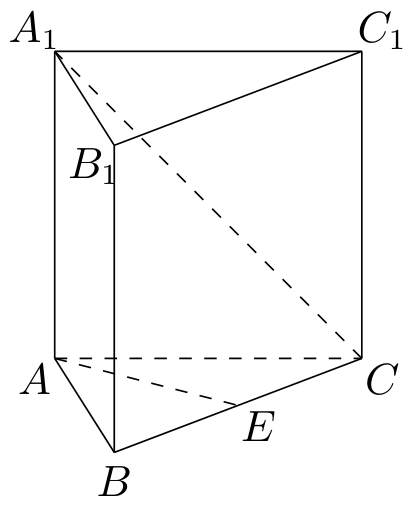
\includegraphics[width=4.2cm]{GaoKao/images/2011/hubei_science/q18_fig1.png}
\end{center}

        \item 已知数列 \(\{a_{n}\}\) 的前 \(n\) 项和为 \(S_{n}\)，且满足 \(a_{1} = a\)，\(a \neq 0\)，\(a_{n+1} = rS_{n}\)，\(n \in \mathbf{N}^{*}\)，\(r \in \mathbb{R}\)，\(r \neq -1\).
\begin{enumerate}
\item 求数列 \( \{a_{n}\} \) 的通项公式；
\item 若存在 \(k \in \mathbf{N}^*\)，使得 \(S_{k+1}\)，\(S_k\)，\(S_{k+2}\) 成等差数列，试判断：对于任意的 \(m \in \mathbf{N}^*\)，且 \(m \geqslant 2\)，\(a_{m+1}\)，\(a_m\)，\(a_{m+2}\) 是否成等差数列，并证明你的结论.
\end{enumerate}

        \item 平面内与两定点 \(A_{1}(-a,0)\)，\(A_{2}(a,0)\)（\(a > 0\)）连线的斜率之积等于非零常数 \(m\) 的点的轨迹. 加上 \(A_{1}\)，\(A_{2}\) 两点所成的曲线 \(C\) 可以是圆，椭圆或双曲线.
\begin{enumerate}
\item 求曲线 \(C\) 的方程，并讨论 \(C\) 的形状与 \(m\) 值的关系；
\item 当 \(m = -1\) 时，对应的曲线为 \(C_1\)；对给定的 \(m \in (-1,0) \cup (0, +\infty)\)，对应的曲线为 \(C_2\). 设 \(F_1\)，\(F_2\) 是 \(C_2\) 的两个焦点. 试问：在 \(C_1\) 上，是否存在点 \(N\)，使得 \(\triangle F_1NF_2\) 的面积 \(S = |m|a^2\)？ 若存在，求 \(\tan \angle F_1NF_2\) 的值；若不存在，请说明理由.
\end{enumerate}

        \item \begin{enumerate}
\item 已知函数 \(f(x) = \ln x - x + 1\)，\(x \in (0, +\infty)\)，求函数 \( f(x) \) 的最大值.

\item 设 \(a_k\)，\(b_k\)（\(k = 1\)，\(2\)，\(\dots\)，\(n\)）均为正数，证明：

\begin{enumerate}
\item 若 \(a_1b_1 + a_2b_2 + \dots + a_nb_n \leqslant b_1 + b_2 + \dots + b_n\)，则 \(a_1^{b_1} a_2^{b_2} \cdots a_n^{b_n} \leqslant 1\)；
\item 若 \(b_{1} + b_{2} + \dots + b_{n} = 1\)，则 \(\frac{1}{n} \leqslant b_{1}^{b_{1}} b_{2}^{b_{2}} \cdots b_{n}^{b_{n}} \leqslant b_{1}^{2} + b_{2}^{2} + \dots + b_{n}^{2}\).
\end{enumerate}
\end{enumerate}

    \end{enumerate}

\end{description}


\subsection{2011年湖北卷（文）}\label{gk:2011年湖北卷（文）}

\begin{description}

    \item[一、选择题]

    \begin{enumerate}[leftmargin=5pt]

        \item 已知 \( U = \{1, 2, 3, 4, 5, 6, 7, 8\} \)， \( A = \{1, 3, 5, 7\} \)， \( B = \{2, 4, 5\} \)，则 \( \complement_{U}(A \cup B) = \)（\quad）

        {\centering\begin{tabular*}{\linewidth}{@{}@{\extracolsep{\fill}}llll@{}}
          \text{A. }\(\{6, 8\}\)  &  \text{B. }\(\{5,7\}\)  &  \text{C. }\( \{4, 6, 7\} \)  &  \text{D. }\(\{1, 3, 5, 6, 8\}\)
        \end{tabular*}\par}

        \item 若向量 \(\bm{a} = (1, 2)\)，\(\bm{b} = (1, -1)\)，则 \(2\bm{a} + \bm{b}\) 与 \(\bm{a} - \bm{b}\) 的夹角等于（\quad）

        {\centering\begin{tabular*}{\linewidth}{@{}@{\extracolsep{\fill}}llll@{}}
          \text{A. }\(-\frac{\pi}{4}\)  &  \text{B. }\( \frac{\pi}{6} \)  &  \text{C. }\( \frac{\pi}{4} \)  &  \text{D. }\(\frac{3\pi}{4}\)
        \end{tabular*}\par}

        \item 若定义在 \(\mathbb{R}\) 上的偶函数 \(f(x)\) 和奇函数 \(g(x)\) 满足 \(f(x) + g(x) = {\mathrm{e}}^{x}\)，则 \(g(x) =\)（\quad）

        {\centering\begin{tabular*}{\linewidth}{@{}@{\extracolsep{\fill}}llll@{}}
          \text{A. }\({\mathrm{e}}^x - {\mathrm{e}}^{-x}\)  &  \text{B. }\(\frac{1}{2} ({\mathrm{e}}^x + {\mathrm{e}}^{-x})\)  &  \text{C. }\(\frac{1}{2} ({\mathrm{e}}^{-x} - {\mathrm{e}}^{x})\)  &  \text{D. }\(\frac{1}{2} ({\mathrm{e}}^{x} - {\mathrm{e}}^{-x})\)
        \end{tabular*}\par}

        \item 将两个顶点在抛物线 \( y^{2} = 2px \)（\(p > 0\)） 上，另一个顶点是此抛物线焦点的正三角形个数记为 \( n \)，则（\quad）

        {\centering\begin{tabular*}{\linewidth}{@{}@{\extracolsep{\fill}}llll@{}}
          \text{A. }\(n = 0\)  &  \text{B. }\(n = 1\)  &  \text{C. }\(n = 2\)  &  \text{D. }\(n \geqslant 3\)
        \end{tabular*}\par}

        \item 有一个容量为 \(200\) 的样本，其频率分布直方图如图所示，根据样本的频率分布直方图估计，样本数据落在区间 \([10,12)\) 内的频数为（\quad）

\begin{center}
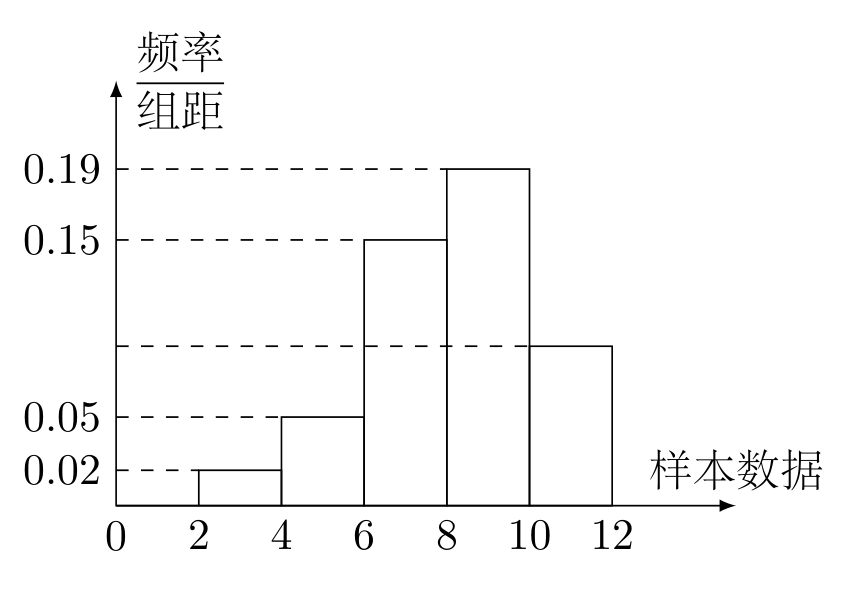
\includegraphics[width=0.42\linewidth]{GaoKao/images/2011/hubei_liberal/q5_fig1.png}
\end{center}

        {\centering\begin{tabular*}{\linewidth}{@{}@{\extracolsep{\fill}}llll@{}}
          \text{A. }\(18\)  &  \text{B. }\(36\)  &  \text{C. }\(54\)  &  \text{D. }\(72\)
        \end{tabular*}\par}

        \item 已知函数 \(f(x) = \sqrt{3}\sin x - \cos x\)，\(x \in \mathbb{R}\). 若 \( f(x) \geqslant 1 \)，则 \( x \) 的取值范围为（\quad）

        {\centering\begin{tabular*}{\linewidth}{@{}@{\extracolsep{\fill}}llll@{}}
          \text{A. }\(\left\{x\mid 2k\pi +\frac{\pi}{3}\leqslant x\leqslant 2k\pi +\pi ,k\in \mathbb{Z}\right\}\)  &  \text{B. }\(\left\{x\mid k\pi +\frac{\pi}{3}\leqslant x\leqslant k\pi +\pi,k\in \mathbb{Z}\right\}\)  &  \text{C. }\(\left\{x\mid 2k\pi +\frac{\pi}{6}\leqslant x\leqslant 2k\pi +\frac{5\pi}{6},k\in \mathbb{Z}\right\}\)  &  \text{D. }\(\left\{x\mid k\pi +\frac{\pi}{6}\leqslant x\leqslant k\pi +\frac{5\pi}{6},k\in \mathbb{Z}\right\}\)
        \end{tabular*}\par}

        \item 设球的体积为 \(V_{1}\). 它的内接正方体的体积为 \(V_{2}\). 下列说法中最合适的是（\quad）

        {\centering\begin{tabular*}{\linewidth}{@{}@{\extracolsep{\fill}}llll@{}}
          \text{A. }\(V_{1}\) 比 \(V_{2}\) 大约多一半  &  \text{B. }\(V_{1}\) 比 \(V_{2}\) 大约多两倍半  &  \text{C. }\(V_{1}\) 比 \(V_{2}\) 大约多一倍  &  \text{D. }\(V_{1}\) 比 \(V_{2}\) 大约多一倍半
        \end{tabular*}\par}

        \item 直线 \(2x + y - 10 = 0\) 与不等式组 \(\begin{cases}
x \geqslant 0,\\
y \geqslant 0,\\
x - y \geqslant -2,\\
4x + 3y \leqslant 20
\end{cases}\) 表示的平面区域的公共点有（\quad）

        {\centering\begin{tabular*}{\linewidth}{@{}@{\extracolsep{\fill}}llll@{}}
          \text{A. }\(0\text{ 个}\)  &  \text{B. }\(1\text{ 个}\)  &  \text{C. }\(2\text{ 个}\)  &  \text{D. }无数个
        \end{tabular*}\par}

        \item 《九章算术》“竹九节”问题：现有一根 \(9\) 节的竹子，自上而下各节的容积成等差数列，上面 \(4\) 节的容积共 \(3\text{ 升}\)，下面 \(3\) 节的容积共 \(4\text{ 升}\)，则第 \(5\) 节的容积为（\quad）

        {\centering\begin{tabular*}{\linewidth}{@{}@{\extracolsep{\fill}}llll@{}}
          \text{A. }\(1\text{ 升}\)  &  \text{B. }\(\frac{67}{66}\text{ 升}\)  &  \text{C. }\(\frac{47}{44}\text{ 升}\)  &  \text{D. }\(\frac{37}{33}\text{ 升}\)
        \end{tabular*}\par}

        \item 若实数 \(a\)，\(b\) 满足 \(a \geqslant 0\)，\(b \geqslant 0\)，且 \(ab = 0\)，则称 \(a\) 与 \(b\) 互补. 记 \(\varphi(a, b) = \sqrt{a^2 + b^2} - a - b\)，那么 \(\varphi(a, b) = 0\) 是 \(a\) 与 \(b\) 互补的（\quad）

        {\centering\begin{tabular*}{\linewidth}{@{}@{\extracolsep{\fill}}llll@{}}
          \text{A. }必要而不充分条件  &  \text{B. }充分而不必要条件  &  \text{C. }充要条件  &  \text{D. }既不充分也不必要条件
        \end{tabular*}\par}

    \end{enumerate}

\end{description}

\begin{description}

    \item[二、填空题]

    \begin{enumerate}[leftmargin=5pt]

      \addtocounter{enumi}{+10}

        \item 某市有大型超市 \(200\text{ 家}\)，中型超市 \(400\text{ 家}\)，小型超市 \(1400\text{ 家}\). 为掌握各类超市的营业情况，现按分层抽样方法抽取一个容量为 \(100\) 的样本，应抽取中型超市\rule[-0.3ex]{3em}{0.4pt} 家.

        \item \(\left(x - \frac{1}{3\sqrt{x}}\right)^{18}\) 的展开式中含 \(x^{15}\) 的项的系数为\rule[-0.3ex]{3em}{0.4pt}. （结果用数值表示）

        \item 在 \(30\) 瓶饮料中，有 \(3\) 瓶已过了保质期. 从这 \(30\) 瓶饮料中任取 \(2\) 瓶，则至少取到 \(1\) 瓶已过保质期饮料的概率为\rule[-0.3ex]{3em}{0.4pt}. （结果用最简分数表示）

        \item 过点 \((-1, -2)\) 的直线 \(t\) 被圆 \(x^{2} + y^{2} - 2x - 2y + 1 = 0\) 截得的弦长为 \(\sqrt{2}\)，则直线 \(t\) 的斜率为\rule[-0.3ex]{3em}{0.4pt}.

        \item 里氏震级 \(M\) 的计算公式为： \(M = \lg A - \lg A_0\). 其中 \(A\) 是测震仪记录的地震曲线的最大振幅，\(A_0\) 是相应的标准地震的振幅. 假设在一次地震中，测震仪记录的最大振幅是 \(1000\)，此时标准地震的振幅为 \(0.001\)，则此次地震的震级为\rule[-0.3ex]{3em}{0.4pt}\(\text{级}\)；\(9\text{ 级}\)地震的最大的振幅是 \(5\text{ 级}\)地震最大振幅的\rule[-0.3ex]{3em}{0.4pt}\(\text{倍}\).

    \end{enumerate}

\end{description}

\begin{description}

    \item[三、解答题]

    \begin{enumerate}[leftmargin=5pt]

      \addtocounter{enumi}{+15}

        \item 设 \(\triangle ABC\) 的内角 \(A\)，\(B\)，\(C\) 所对的边分别为 \(a\)，\(b\)，\(c\). 已知 \(a = 1\)，\(b = 2\)，\(\cos C = \frac{1}{4}\).
\begin{enumerate}
\item 求 \( \triangle ABC \) 的周长；
\item 求 \( \cos(A-C) \) 的值.
\end{enumerate}

        \item 成等差数列的三个正数的和等于 \(15\)，并且这三个数分别加上 \(2\)，\(5\)，\(13\) 后成为等比数列 \(\{b_n\}\) 中的 \(b_3\)，\(b_4\)，\(b_5\).
\begin{enumerate}
\item 求数列 \( \{b_{n}\} \) 的通项公式；
\item 数列 \( \{b_{n}\} \) 的前 \(n\) 项和为 \( S_{n} \)，求证：数列 \( \left\{S_{n}+\frac{5}{4}\right\} \) 是等比数列.
\end{enumerate}

        \item 如图，已知正三棱柱 \(ABC - A_{1}B_{1}C_{1}\) 的底面边长为 \(2\)，侧棱长为 \(3\sqrt{2}\)，点 \(E\) 在侧棱 \(AA_{1}\) 上，点 \(F\) 在侧棱 \(BB_{1}\) 上，且 \(AE = 2\sqrt{2}\)，\(BF = \sqrt{2}\).

\begin{enumerate}
\item 求证：\(CF \perp C_{1}E\).
\item 求二面角 \(E - CF - C_1\) 的大小.
\end{enumerate}

\begin{center}
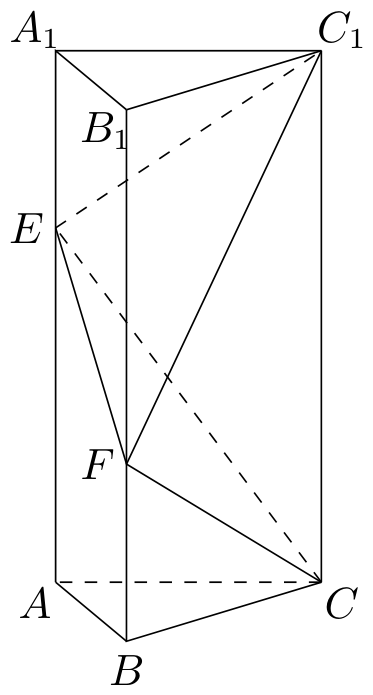
\includegraphics[width=3.7cm]{GaoKao/images/2011/hubei_liberal/q18_fig1.png}
\end{center}

        \item 提高过江大桥的车辆通行能力可改善整个城市的交通状况. 在一般情况下，大桥上的车流速度 \(v\)（单位：千米/小时）是车流密度 \(x\)（单位：辆/千米）的函数. 当桥上的车流密度达到 \(200\text{ 辆/千米}\) 时，造成堵塞，此时车流速度为 \(0\)；当车流密度不超过 \(20\text{ 辆/千米}\) 时，车流速度为 \(60\text{ 千米/小时}\). 研究表明：当 \(20 \leqslant x \leqslant 200\) 时，车流速度 \(v\) 是车流密度 \(x\) 的一次函数.
\begin{enumerate}
\item 当 \(0 \leqslant x \leqslant 200\) 时，求函数 \(v(x)\) 的表达式；
\item 当车流密度 \(x\) 为多大时，车流量（单位时间内通过桥上某观测点的车辆数，单位：辆/小时）\(f(x) = x \cdot v(x)\) 可以达到最大，并求出最大值. （精确到 \(1\text{ 辆/小时}\)）
\end{enumerate}

        \item 设函数 \( f(x) = x^{3} + 2ax^{2} + bx + a \)，\( g(x) = x^{2} - 3x + 2 \)，其中 \( x \in \mathbb{R} \)，\(a\)，\(b\) 为常数，已知曲线 \( y = f(x) \) 与 \( y = g(x) \) 在点 \((2,0)\) 处有相同的切线 \( l \).
\begin{enumerate}
\item 求 \(a\)，\(b\) 的值，并写出切线 \(l\) 的方程；
\item 若方程 \( f(x) + g(x) = mx \) 有三个互不相同的实根 \(0\)，\(x_1\)，\(x_2\)，其中 \( x_1 < x_2 \)，且对任意的 \( x \in [x_1, x_2] \)，\( f(x) + g(x) < m (x - 1) \) 恒成立，求实数 \( m \) 的取值范围.
\end{enumerate}

        \item 平面内与两定点 \(A_{1}(-a,0)\)，\(A_{2}(a,0) \)（\(a > 0\)） 连线的斜率之积等于非零常数 \(m\) 的点的轨迹，加上 \(A_{1}\)，\(A_{2}\) 两点所成的曲线 \(C\) 可以是圆，椭圆或双曲线.
\begin{enumerate}
\item 求曲线 C 的方程，并讨论 C 的形状与 m 值的关系；
\item 当 \(m = -1\) 时，对应的曲线为 \(C_1\)；对给定的 \(m \in (-1,0) \cup (0,+\infty)\)，对应的曲线为 \(C_2\). 设 \(F_1\)，\(F_2\) 是 \(C_2\) 的两个焦点. 试问：在 \(C_1\) 上，是否存在点 \(N\)，使得 \(\triangle F_1NF_2\) 的面积 \(S = |m|a^2\)？若存在，求 \(\tan \angle F_1NF_2\) 的值；若不存在，请说明理由.
\end{enumerate}

    \end{enumerate}

\end{description}


\subsection{2011年湖南卷（理）}\label{gk:2011年湖南卷（理）}

\begin{description}

    \item[一、选择题]

    \begin{enumerate}[leftmargin=5pt]

        \item 若 \(a,b \in \mathbb{R}\)，\(\i\) 为虚数单位，且 \((a + \i)\i = b + \i\)，则（\quad）

        {\centering\begin{tabular*}{\linewidth}{@{}@{\extracolsep{\fill}}llll@{}}
          \text{A. }\(a = 1\)，\(b = 1\)  &  \text{B. }\(a = -1\)，\(b = 1\)  &  \text{C. }\(a = -1\)，\(b = -1\)  &  \text{D. }\(a = 1\)，\(b = -1\)
        \end{tabular*}\par}

        \item 设 \(M = \{1, 2\}\)，\(N = \{a^2\}\)，则 “\(a = 1\)” 是 “\(N \subseteq M\)” 的（\quad）

        {\centering\begin{tabular*}{\linewidth}{@{}@{\extracolsep{\fill}}llll@{}}
          \text{A. }充分不必要条件  &  \text{B. }必要不充分条件  &  \text{C. }充分必要条件  &  \text{D. }既不充分又不必要条件
        \end{tabular*}\par}

        \item 如图是某几何体的三视图，则该几何体的体积为（\quad）

\begin{center}
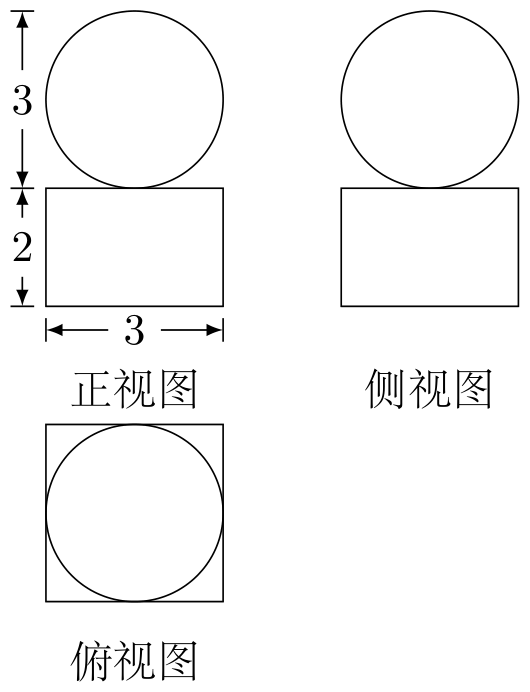
\includegraphics[width=2.1cm]{GaoKao/images/2011/hunan_science/q3_fig1.png}
\end{center}

        {\centering\begin{tabular*}{\linewidth}{@{}@{\extracolsep{\fill}}llll@{}}
          \text{A. }\(\frac{9}{2}\pi + 12\)  &  \text{B. }\(\frac{9}{2}\pi + 18\)  &  \text{C. }\(9\pi + 42\)  &  \text{D. }\(36\pi + 18\)
        \end{tabular*}\par}

        \item 通过随机询问 \(110\text{ 名}\) 性别不同的大学生是否爱好某项运动，得到如下的列联表：

\begin{center}
\begin{tabular}{c|ccc}
 & 男 & 女 & 总计 \\
\hline
爱好 & 40 & 20 & 60 \\
不爱好 & 20 & 30 & 50 \\
总计 & 60 & 50 & 110
\end{tabular}
\end{center}

由 \(K^2 = \frac{n(ad - bc)^2}{(a + b)(c + d)(a + c)(b + d)}\) 算得 \(K^{2} = \frac{110 \times (40 \times 30 - 20 \times 20)^{2}}{60 \times 50 \times 60 \times 50} \approx 7.8\). 附表：

\begin{center}
\begin{tabular}{c|ccc}
\(P(K^2\geqslant k)\) & 0.050 & 0.010 & 0.001 \\
\hline
\(k\) & 3.841 & 6.635 & 10.828
\end{tabular}
\end{center}

参照附表，得到的正确结论是（\quad）

        {\centering\begin{tabular*}{\linewidth}{@{}@{\extracolsep{\fill}}llll@{}}
          \text{A. }在犯错误的概率不超过 \(0.1\%\) 的前提下，认为“爱好该项运动与性别有关”  &  \text{B. }在犯错误的概率不超过 \(0.1\%\) 的前提下，认为“爱好该项运动与性别无关”  &  \text{C. }有 \(99\%\) 以上的把握认为“爱好该项运动与性别有关”  &  \text{D. }有 \(99\%\) 以上的把握认为“爱好该项运动与性别无关”
        \end{tabular*}\par}

        \item 设双曲线 \(\frac{x^2}{a^2} - \frac{y^2}{9} = 1\)（\(a > 0\)）的渐近线方程为 \(3x \pm 2y = 0\)，则 \(a\) 的值为（\quad）

        {\centering\begin{tabular*}{\linewidth}{@{}@{\extracolsep{\fill}}llll@{}}
          \text{A. }4  &  \text{B. }3  &  \text{C. }2  &  \text{D. }1
        \end{tabular*}\par}

        \item 由直线 \(x = -\frac{\pi}{3}\)，\(x = \frac{\pi}{3}\)，\(y = 0\) 与曲线 \(y = \cos x\) 所围成的封闭图形的面积为（\quad）

        {\centering\begin{tabular*}{\linewidth}{@{}@{\extracolsep{\fill}}llll@{}}
          \text{A. }\(\frac{1}{2}\)  &  \text{B. }1  &  \text{C. }\(\frac{\sqrt{3}}{2}\)  &  \text{D. }\(\sqrt{3}\)
        \end{tabular*}\par}

        \item 设 \(m > 1\)，在约束条件 \(\begin{cases}
y \geqslant x,\\
y \leqslant mx,\\
x + y \leqslant 1
\end{cases}\) 下，目标函数 \(z = x + my\) 的最大值小于 \(2\)，则 \(m\) 的取值范围为（\quad）

        {\centering\begin{tabular*}{\linewidth}{@{}@{\extracolsep{\fill}}llll@{}}
          \text{A. }\((1, 1 + \sqrt{2})\)  &  \text{B. }\((1 + \sqrt{2}, +\infty)\)  &  \text{C. }\((1,3)\)  &  \text{D. }\((3, +\infty)\)
        \end{tabular*}\par}

        \item 设直线 \(x = t\) 与函数 \(f(x) = x^2\)，\(g(x) = \ln x\) 的图象分别交于点 \(M\)，\(N\)，则当 \(|MN|\) 达到最小时 \(t\) 的值为（\quad）

        {\centering\begin{tabular*}{\linewidth}{@{}@{\extracolsep{\fill}}llll@{}}
          \text{A. }1  &  \text{B. }\( \frac{1}{2} \)  &  \text{C. }\(\frac{\sqrt{5}}{2}\)  &  \text{D. }\(\frac{\sqrt{2}}{2}\)
        \end{tabular*}\par}

    \end{enumerate}

\end{description}

\begin{description}

    \item[二、填空题]

    \begin{enumerate}[leftmargin=5pt]

      \addtocounter{enumi}{+8}

        \item 在直角坐标系 \(xOy\) 中，曲线 \(C_1\) 的参数方程为 \(\begin{cases}
x = \cos \alpha,\\
y = 1 + \sin \alpha
\end{cases}\) （\(\alpha\) 为参数），在极坐标系（与直角坐标系 \(xOy\) 取相同的长度单位，且以原点 \(O\) 为极点，以 \(x\) 轴正半轴为极轴）中，曲线 \(C_2\) 的方程为 \(\rho (\cos \theta - \sin \theta) + 1 = 0\)，则 \(C_1\) 与 \(C_2\) 的交点个数为\rule[-0.3ex]{3em}{0.4pt}.

        \item 设 \(x,y \in \mathbb{R}\)，且 \(xy \neq 0\)，则 \(\left(x^2 + \frac{1}{y^2}\right)\left(\frac{1}{x^2} + 4y^2\right)\) 的最小值为\rule[-0.3ex]{3em}{0.4pt}.

        \item 如图，\(A\)，\(E\) 是半圆周上的两个三等分点，直径 \(BC=4\)，\(AD\perp BC\)，垂足为 \(D\)，\(BE\) 与 \(AD\) 相交于点 \(F\)，则 \(AF\) 的长为\rule[-0.3ex]{3em}{0.4pt}.

\begin{center}
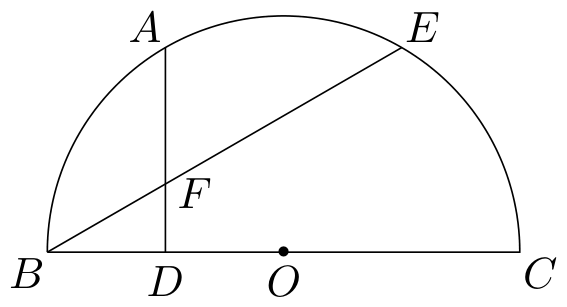
\includegraphics[width=7.0cm]{GaoKao/images/2011/hunan_science/q11_fig1.png}
\end{center}

        \item 设 \(S_{n}\) 是等差数列 \(\{a_{n}\}\)（\(n \in \mathbf{N}^{*}\)）的前 \(n\) 项和，且 \(a_{1} = 1\)，\(a_{4} = 7\)，则 \(S_{5} =\)\rule[-0.3ex]{3em}{0.4pt}.

        \item 若执行如图所示的框图，输入 \(x_{1} = 1\)，\(x_{2} = 2\)，\(x_{3} = 3\)，\(\overline{x} = 2\)，则输出的数等于\rule[-0.3ex]{3em}{0.4pt}.

\begin{center}
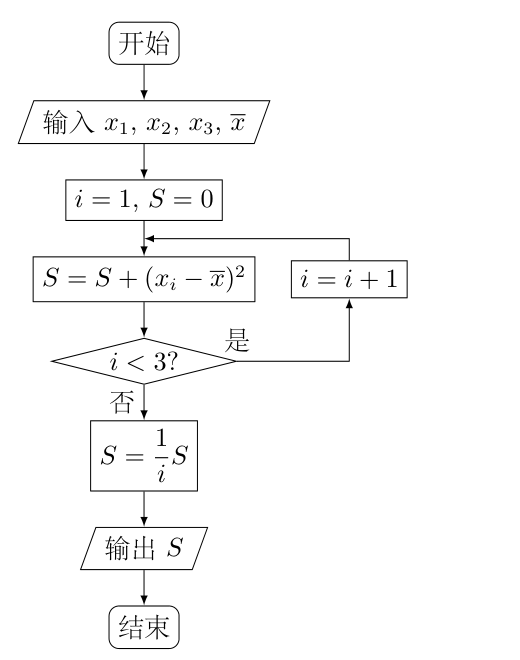
\includegraphics[width=0.32\linewidth]{GaoKao/images/2011/hunan_science/q13_fig1.png}
\end{center}

        \item 在边长为 1 的正三角形 \(ABC\) 中，设 \(\overrightarrow{BC} = 2\overrightarrow{BD}\)，\(\overrightarrow{CA} = 3\overrightarrow{CE}\)，则 \(\overrightarrow{AD} \cdot \overrightarrow{BE} =\)\rule[-0.3ex]{3em}{0.4pt}.

        \item 如图所示，\(EFGH\) 是以 \(O\) 为圆心，半径为 1 的圆的内接正方形，将一颗豆子随机地扔到该圆内，用 \(A\) 表示事件“豆子落在正方形 \(EFGH\) 内”，\(B\) 表示事件“豆子落在扇形 \(OHE\)（阴影部分）内”，则
\begin{enumerate}
\item \(P(A)=\)\rule[-0.3ex]{3em}{0.4pt}；
\item \(P(B|A)=\)\rule[-0.3ex]{3em}{0.4pt}.
\end{enumerate}

\begin{center}
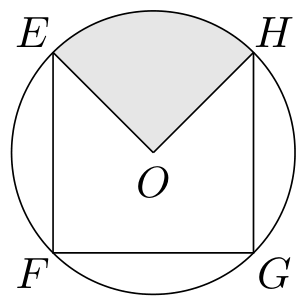
\includegraphics[width=3.7cm]{GaoKao/images/2011/hunan_science/q15_fig1.png}
\end{center}

        \item 对于 \(n \in \mathbf{N}^*\)，将 \(n\) 表示为 \(n = a_0 \times 2^k + a_1 \times 2^{k-1} + a_2 \times 2^{k-2} + \cdots + a_{k-1} \times 2^1 + a_k \times 2^0\). 当 \(i = 0\) 时，\(a_i = 1\)，当 \(1 \leqslant i \leqslant k\) 时，\(a_i\) 为 0 或 1. 记 \(I(n)\) 为上述表示中 \(a_i\) 为 0 的个数 （例如： \(1 = 1 \times 2^0\)，\(4 = 1 \times 2^2 + 0 \times 2^1 + 0 \times 2^0\)，则 \(I(1) = 0\)，\(I(4) = 2\)），则
\begin{enumerate}
    \item \(I(12) =\)\rule[-0.3ex]{3em}{0.4pt}；
    \item \(\displaystyle\sum_{n=1}^{127} 2^{I(n)}=\)\rule[-0.3ex]{3em}{0.4pt}.
\end{enumerate}

    \end{enumerate}

\end{description}

\begin{description}

    \item[三、解答题]

    \begin{enumerate}[leftmargin=5pt]

      \addtocounter{enumi}{+16}

        \item 在 \(\triangle ABC\) 中，角 \(A\)，\(B\)，\(C\) 所对的边分别为 \(a\)，\(b\)，\(c\). 且满足 \(c \sin A = a \cos C\).
\begin{enumerate}
\item 求角 \(C\) 的大小；
\item 求 \(\sqrt{3} \sin A - \cos \left(B + \frac{\pi}{4}\right)\) 的最大值，并求取得最大值时角 A，B 的大小.
\end{enumerate}

        \item 某商店试销某种商品 \(20\text{ 天}\)，获得如下数据：

\begin{center}
\begin{tabular}{c|cccc}
日销售量（件） & 0 & 1 & 2 & 3 \\
\hline
频数 & 1 & 5 & 9 & 5
\end{tabular}
\end{center}

试销结束后（假设该商品的日销售量的分布规律不变），设某天开始营业时有该商品 \(3\text{ 件}\)，当天营业结束后检查存货，若发现存货少于 \(2\text{ 件}\)，则当天进货补充至 \(3\text{ 件}\)，否则不进货，将频率视为概率.

\begin{enumerate}
\item 求当天商品不进货的概率；
\item 记 \(X\) 为第二天开始营业时该商品的件数，求 \(X\) 的分布列和数学期望.
\end{enumerate}

        \item 如图，在圆锥 \(PO\) 中，已知 \(PO = \sqrt{2}\)，\(\odot O\) 的直径 \(AB = 2\)，\(C\) 是 \(\widehat{AB}\) 的中点，\(D\) 为 \(AC\) 的中点.
\begin{enumerate}
\item 证明：平面 \(POD \perp\) 平面 \(PAC\)；
\item 求二面角 \(B - PA - C\) 的余弦值.
\end{enumerate}

\begin{center}
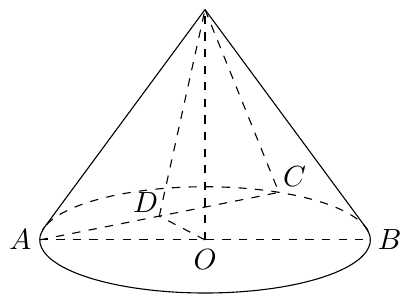
\includegraphics[width=6.9cm]{GaoKao/images/2011/hunan_science/q19_fig1.png}
\end{center}

        \item 如图，长方体物体 \(E\) 在雨中沿面 \(P\)（面积为 \(S\)）的垂直方向作匀速移动，速度为 \(v\)（\(v > 0\)），雨速沿 \(E\) 移动方向的分速度为 \(c\)（\(c \in \mathbb{R}\)）. \(E\) 移动时单位时间内的淋雨量包括两部分：
\begin{enumerate}
\item \(P\) 或 \(P\) 的平行面 （只有一个面淋雨） 的淋雨量，假设其值与 \(|v - c| \times S\) 成正比，比例系数为 \(\frac{1}{10}\)；
\item 其它面的淋雨量之和，其值为 \(\frac{1}{2}\)；
\end{enumerate}
记 \(y\) 为 \(E\) 移动过程中的总淋雨量，当移动距离 \(d = 100\)，面积 \(S = \frac{3}{2}\) 时.
\begin{enumerate}
\item 写出 \(y\) 的表达式；
\item 设 \(0 < v \leqslant 10\)，\(0 < c \leqslant 5\)，试根据 \(c\) 的不同取值范围，确定移动速度 \(v\)，使 \(y\) 最少.
\end{enumerate}


\begin{center}
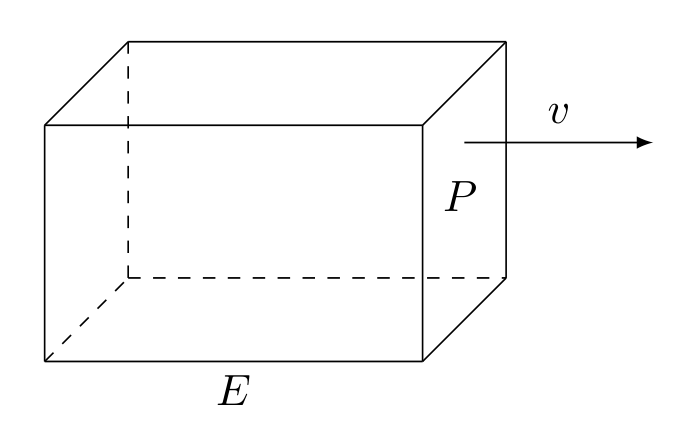
\includegraphics[width=5.3cm]{GaoKao/images/2011/hunan_science/q20_fig1.png}
\end{center}

        \item 如图，椭圆 \(C_{1}:\frac{x^{2}}{a^{2}} +\frac{y^{2}}{b^{2}} = 1\)（\(a > b > 0\)）的离心率为 \(\frac{\sqrt{3}}{2}\)，\(x\) 轴被曲线 \(C_2\)：\(y = x^{2} - b\) 截得的线段长等于 \(C_1\) 的长半轴长.
\begin{enumerate}
\item 求 \(C_1\)，\(C_2\) 的方程；
\item 设 \(C_2\) 与 \(y\) 轴的交点为 \(M\)，过坐标原点 \(O\) 的直线 \(l\) 与 \(C_2\) 相交于点 \(A\)，B，直线 \(MA\)，\(MB\) 分别与 \(C_1\) 相交于点 \(D\)，\(E\).
\begin{enumerate}
\item 证明：\(MD \perp ME\)；
\item 记 \(\triangle MAB\)，\(\triangle MDE\) 的面积分别是 \(S_{1}\)，\(S_{2}\). 问：是否存在直线 \(l\)，使得 \(\frac{S_{1}}{S_{2}} = \frac{17}{32}\)，请说明理由.
\end{enumerate}
\end{enumerate}

\begin{center}
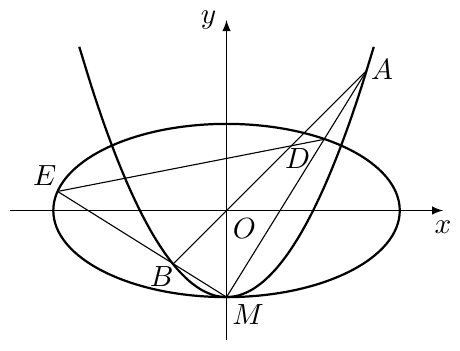
\includegraphics[width=8.6cm]{GaoKao/images/2011/hunan_science/q21_fig1.png}
\end{center}

        \item 已知函数 \(f(x) = x^3\)，\(g(x) = x + \sqrt{x}\).
\begin{enumerate}
\item 求函数 \( h(x) = f(x) - g(x) \) 的零点个数，并说明理由；
\item 设数列 \(\{a_{n}\}\)（\(n \in \mathbf{N}^{*}\)）满足 \(a_{1} = a\)（\(a > 0\)），\(f(a_{n+1}) = g(a_{n})\)，证明：存在常数 \(M\)，使得对于任意的 \(n \in \mathbf{N}^{*}\)，都有 \(a_{n} \leqslant M\).
\end{enumerate}

    \end{enumerate}

\end{description}


\subsection{2011年湖南卷（文）}\label{gk:2011年湖南卷（文）}

\begin{description}

    \item[一、选择题]

    \begin{enumerate}[leftmargin=5pt]

        \item 设全集 \(U = M \cup N = \{1, 2, 3, 4, 5\}\)，\(M \cap \complement_U N = \{2, 4\}\)，则 \(N =\)（\quad）

        {\centering\begin{tabular*}{\linewidth}{@{}@{\extracolsep{\fill}}llll@{}}
          \text{A. }\(\{1, 2, 3\}\)  &  \text{B. }\(\{1,3,5\}\)  &  \text{C. }\(\{1,4,5\}\)  &  \text{D. }\(\{2,3,4\}\)
        \end{tabular*}\par}

        \item 若 \(a,b\in\mathbb{R}\)，\(\i\) 为虚数单位，且 \((a + \i)\i = b + \i\)，则（\quad）

        {\centering\begin{tabular*}{\linewidth}{@{}@{\extracolsep{\fill}}llll@{}}
          \text{A. }\(a = 1\)，\(b = 1\)  &  \text{B. }\(a = -1\)，\(b = 1\)  &  \text{C. }\(a = 1\)，\(b = -1\)  &  \text{D. }\(a = -1\)，\(b = -1\)
        \end{tabular*}\par}

        \item “\(x>1\)”是“\(|x|>1\)”的（\quad）

        {\centering\begin{tabular*}{\linewidth}{@{}@{\extracolsep{\fill}}llll@{}}
          \text{A. }充分不必要条件  &  \text{B. }必要不充分条件  &  \text{C. }充分必要条件  &  \text{D. }既不充分又不必要条件
        \end{tabular*}\par}

        \item 如图是某几何体的三视图，则该几何体的体积为

\begin{center}
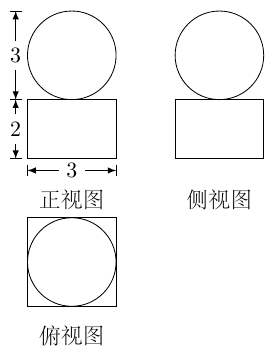
\includegraphics[width=2.2cm]{GaoKao/images/2011/hunan_liberal/q4_fig1.png}
\end{center}

        {\centering\begin{tabular*}{\linewidth}{@{}@{\extracolsep{\fill}}llll@{}}
          \text{A. }\(9\pi + 42\)  &  \text{B. }\(36\pi + 18\)  &  \text{C. }\(\frac{9}{2}\pi + 12\)  &  \text{D. }\(\frac{9}{2}\pi + 18\)
        \end{tabular*}\par}

        \item 通过随机询问 \(110\) 名性别不同的大学生是否爱好某项运动，得到如下的列联表：
\begin{center}
\begin{tabular}{c|ccc}
 & 男 & 女 & 总计 \\
\hline
爱好 & \(40\) & \(20\) & \(60\) \\
不爱好 & \(20\) & \(30\) & \(50\) \\
\hline
总计 & \(60\) & \(50\) & \(110\)
\end{tabular}
\end{center}
由 \(K^2 = \frac{n(ad-bc)^2}{(a + b)(c + d)(a + c)(b + d)}\) 算得，\(K^2 = \frac {110 \times (40 \times 30 - 20 \times 20) ^{2}}{60 \times 50 \times 60 \times 50} \approx 7.8\). 附表：
\begin{center}
\begin{tabular}{c|ccc}
\(P(K^2 \geqslant k)\) & \(0.050\) & \(0.010\) & \(0.001\) \\
\hline
\(k\) & \(3.841\) & \(6.635\) & \(10.828\)
\end{tabular}
\end{center}
参照附表，得到的正确结论是（\quad）

        {\centering\begin{tabular*}{\linewidth}{@{}@{\extracolsep{\fill}}llll@{}}
          \text{A. }有 \(99\%\) 以上的把握认为“爱好该项运动与性别有关”  &  \text{B. }有 \(99\%\) 以上的把握认为“爱好该项运动与性别无关”  &  \text{C. }在犯错误的概率不超过 0.1\% 的前提下，认为“爱好该项运动与性别有关”  &  \text{D. }在犯错误的概率不超过 0.1\% 的前提下，认为“爱好该项运动与性别无关”
        \end{tabular*}\par}

        \item 设双曲线 \(\frac{x^2}{a^2} - \frac{y^2}{9} = 1 \) （\(a > 0\)）的渐近线方程为 \(3x \pm 2y = 0\)，则 \(a\) 的值为（\quad）

        {\centering\begin{tabular*}{\linewidth}{@{}@{\extracolsep{\fill}}llll@{}}
          \text{A. }4  &  \text{B. }3  &  \text{C. }2  &  \text{D. }1
        \end{tabular*}\par}

        \item 曲线 \( y = \frac{\sin x}{\sin x + \cos x} - \frac{1}{2} \) 在点 \( M\left(\frac{\pi}{4}, 0\right) \) 处的切线的斜率为（\quad）

        {\centering\begin{tabular*}{\linewidth}{@{}@{\extracolsep{\fill}}llll@{}}
          \text{A. }\(-\frac{1}{2}\)  &  \text{B. }\( \frac{1}{2} \)  &  \text{C. }\( -\frac{\sqrt{2}}{2} \)  &  \text{D. }\( \frac{\sqrt{2}}{2} \)
        \end{tabular*}\par}

        \item 已知函数 \(f(x) = {\mathrm{e}}^{x} - 1\)，\(g(x) = -x^{2} + 4x - 3\)，若有 \( f(a) = g(b) \)，则 \( b \) 的取值范围为（\quad）

        {\centering\begin{tabular*}{\linewidth}{@{}@{\extracolsep{\fill}}llll@{}}
          \text{A. }\([2 - \sqrt{2}, 2 + \sqrt{2}]\)  &  \text{B. }\((2 - \sqrt{2}, 2 + \sqrt{2})\)  &  \text{C. }\([1,3]\)  &  \text{D. }\((1,3)\)
        \end{tabular*}\par}

    \end{enumerate}

\end{description}

\begin{description}

    \item[二、选做题]

    \begin{enumerate}[leftmargin=5pt]

      \addtocounter{enumi}{+8}

        \item \textbf{【选修4-4：坐标系与参数方程】}

在直角坐标系 \(xOy\) 中，曲线 \(C_1\) 的参数方程为 \(\begin{cases}
x = 2\cos \alpha,\\
y = \sqrt{3}\sin \alpha,
\end{cases}\)（\(\alpha\) 为参数）在极坐标系（与直角坐标系 \(xOy\) 取相同的长度单位，且以原点 \(O\) 为极点，以 \(x\) 轴正半轴为极轴）中，曲线 \(C_2\) 的方程为 \(\rho(\cos \theta - \sin \theta) + 1 = 0\)，则 \(C_1\) 与 \(C_2\) 的交点个数为\rule[-0.3ex]{3em}{0.4pt}.

        \item 已知某试验范围为 \([10,90]\)，若用分数法进行 \(4\) 次优选试验，则第二次试点可以是\rule[-0.3ex]{3em}{0.4pt}.

    \end{enumerate}

\end{description}

\begin{description}

    \item[三、填空题]

    \begin{enumerate}[leftmargin=5pt]

      \addtocounter{enumi}{+10}

        \item 若执行如图所示的框图，输入 \(x_{1} = 1\)，\(x_{2} = 2\)，\(x_{3} = 4\)，\(x_{4} = 8\)，则输出的数等于\rule[-0.3ex]{3em}{0.4pt}.

\begin{center}
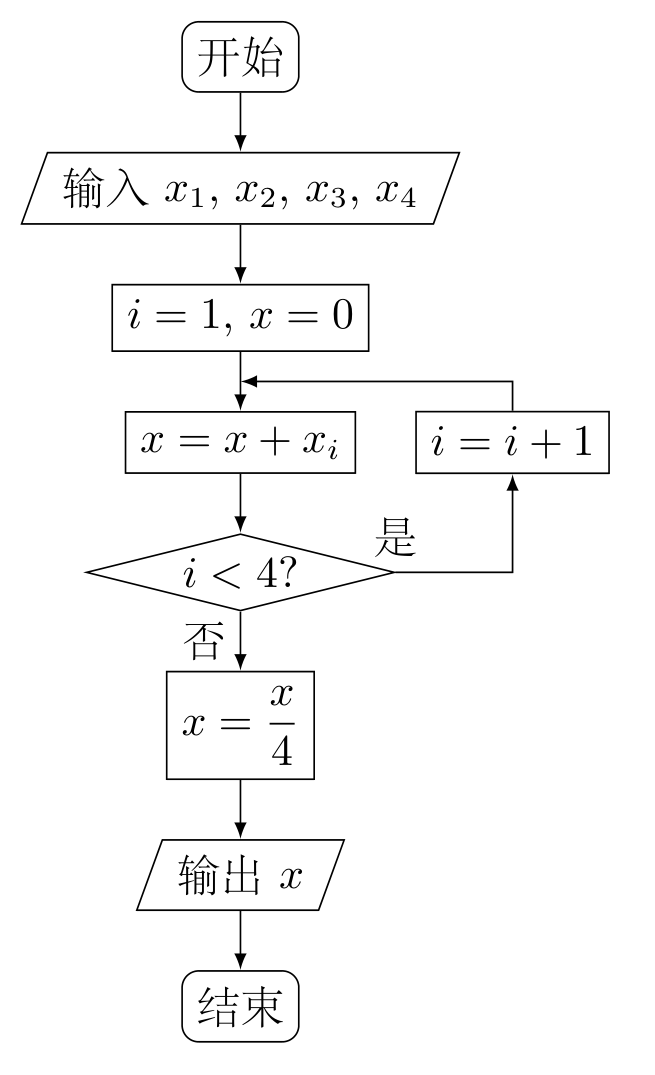
\includegraphics[width=0.30\linewidth]{GaoKao/images/2011/hunan_liberal/q11_fig1.png}
\end{center}

        \item 已知 \( f(x) \) 为奇函数，\( g(x) = f(x) + 9 \)，\( g(-2) = 3 \)，则 \( f(2) = \)\rule[-0.3ex]{3em}{0.4pt}.

        \item 设向量 \(\bm{a}\)，\(\bm{b}\) 满足 \(|\bm{a}| = 2\sqrt{5}\)，\(\bm{b} = (2, 1)\)，且 \(\bm{a}\) 与 \(\bm{b}\) 的方向相反，则 \(\bm{a}\) 的坐标为\rule[-0.3ex]{3em}{0.4pt}.

        \item 设 \(m > 1\)，在约束条件 \(\begin{cases}
y \geqslant x,\\
y \leqslant mx,\\
x + y \leqslant 1
\end{cases}\) 下目标函数 \(z = x + 5y\) 的最大值为 \(4\)，则 \(m\) 的值为\rule[-0.3ex]{3em}{0.4pt}.

        \item 已知圆 \(C: x^{2} + y^{2} = 12\)，直线 \(l: 4x + 3y = 25\).
\begin{enumerate}
\item 圆 \(C\) 的圆心到直线 \(l\) 的距离为\rule[-0.3ex]{3em}{0.4pt}；
\item 圆 \(C\) 上任意一点 \(A\) 到直线 \(l\) 的距离小于 2 的概率为\rule[-0.3ex]{3em}{0.4pt}.
\end{enumerate}

        \item 给定 \(k \in \mathbb{N}^*\)，设函数 \(f: \mathbb{N}^* \to \mathbb{N}^*\) 满足：对于任意大于 \(k\) 的正整数 \(n\)，\(f(n) = n - k\).
\begin{enumerate}
\item 设 \(k = 1\)，则其中一个函数 \(f\) 在 \(n = 1\) 处的函数值为\rule[-0.3ex]{3em}{0.4pt}；
\item 设 \(k = 4\)，且当 \(n \leqslant 4\) 时，\(2 \leqslant f(n) \leqslant 3\)，则不同的函数 \(f\) 的个数为\rule[-0.3ex]{3em}{0.4pt}.
\end{enumerate}

    \end{enumerate}

\end{description}

\begin{description}

    \item[四、解答题]

    \begin{enumerate}[leftmargin=5pt]

      \addtocounter{enumi}{+16}

        \item 在 \(\triangle ABC\) 中，角 \(A\)，\(B\)，\(C\) 所对的边分别为 \(a\)，\(b\)，\(c\)，且满足 \(c \sin A = a \cos C\).
\begin{enumerate}
\item 求角 \(C\) 的大小；
\item 求 \( \sqrt{3}\sin A - \cos\left(B + \frac{\pi}{4}\right) \) 的最大值，并求取得最大值时角 \(A\)，\(B\) 的大小.
\end{enumerate}

        \item 某河流上的一座水力发电站，每年六月份的发电量 \(Y\)（单位：\(\text{万千瓦时}\)）与该河上游在六月份的降雨量 \(X\)（单位：\(\text{毫米}\)）有关，据统计，当 \(X = 70\) 时，\(Y = 460\)；\(X\) 每增加 \(10\)，\(Y\) 增加 \(5\). 已知近 \(20\) 年 \(X\) 的值为：\(140\)，\(110\)，\(160\)，\(70\)，\(200\)，\(160\)，\(140\)，\(160\)，\(220\)，\(200\)，\(110\)，\(160\)，\(160\)，\(200\)，\(140\)，\(110\)，\(160\)，\(220\)，\(140\)，\(160\).

\begin{enumerate}
\item 完成如下的频率分布表：

\begin{center}
\begin{tabular}{c|cccccc}
降雨量 & \(70\) & \(110\) & \(140\) & \(160\) & \(200\) & \(220\) \\
\hline
频率 & \(\frac{1}{20}\) &\rule[-0.3ex]{3em}{0.4pt} & \(\frac{4}{20}\) &\rule[-0.3ex]{3em}{0.4pt} &\rule[-0.3ex]{3em}{0.4pt} & \(\frac{2}{20}\)
\end{tabular}
\end{center}

\item 假定今年六月份的降雨量与近 \(20\) 年六月份降雨量的分布规律相同，并将频率视为概率，求今年六月份该水力发电站的发电量低于 \(490\text{ 万千瓦时}\) 或超过 \(530\text{ 万千瓦时}\) 的概率.
\end{enumerate}

        \item 如图，在圆锥 \(PO\) 中，已知 \(PO = \sqrt{2}\)，\(\odot O\) 的直径 \(AB = 2\)，点 \(C\) 在 \(\widehat{AB}\) 上，且 \(\angle CAB = 30^{\circ}\)，\(D\) 为 \(AC\) 的中点.

\begin{enumerate}
\item 证明： \(AC \perp\) 平面 \(POD\)；
\item 求直线 \(OC\) 和平面 \(PAC\) 所成角的正弦值.
\end{enumerate}

\begin{center}
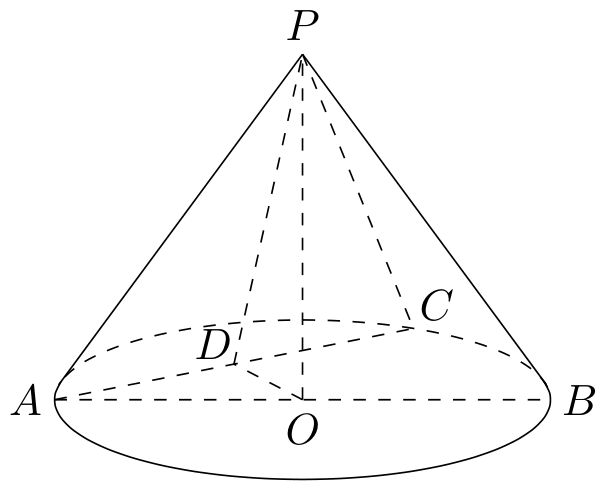
\includegraphics[width=7.0cm]{GaoKao/images/2011/hunan_liberal/q19_fig1.png}
\end{center}

        \item 某企业在第\(1\)年初购买一台价值为 \(120\text{ 万元}\) 的设备 \(M\)，\(M\) 的价值在使用过程中逐年减少. 从第\(2\)年到第\(6\)年，每年初 \(M\) 的价值比上年初减少 \(10\text{ 万元}\)；从第\(7\)年开始，每年初 \(M\) 的价值为上年初的 \(75\%\).
\begin{enumerate}
\item 求第 \(n\) 年初 \(M\) 的价值 \(a_{n}\) 的表达式；
\item 设 \(A_{n} = \frac{a_{1} + a_{2} + \cdots + a_{n}}{n}\)，若 \(A_{n}\) 大于 \(80\text{ 万元}\)，则 \(M\) 继续使用，否则须在第\(n\)年初对 \(M\) 更新，证明：须在第\(9\)年初对 \(M\) 更新.
\end{enumerate}

        \item 已知平面内一动点 \(P\) 到点 \(F(1,0)\) 的距离与点 \(P\) 到 \(y\) 轴的距离的差等于 \(1\).
\begin{enumerate}
\item 求动点 \(P\) 的轨迹 \(C\) 的方程；
\item 过点 \(F\) 作两条斜率存在且互相垂直的直线 \(l_{1}\)，\(l_{2}\)，设 \(l_{1}\) 与轨迹 \(C\) 相交于点 \(A\)，\(B\)，\(l_{2}\) 与轨迹 \(C\) 相交于点 \(D\)，\(E\)，求 \(\overrightarrow{AD} \cdot \overrightarrow{EB}\) 的最小值.
\end{enumerate}

        \item 设函数 \( f(x) = x - \frac{1}{x} - a \ln x  \)（\(a \in \mathbb{R}\)）.
\begin{enumerate}
\item 讨论函数 \( f(x) \) 的单调性.
\item 若 \( f(x) \) 有两个极值点 \( x_{1} \) 和 \( x_{2} \)，记过点 \( A(x_{1}, f(x_{1})) \)，\( B(x_{2}, f(x_{2})) \) 的直线斜率为 \( k \). 问：是否存在 \( a \)，使得 \( k = 2 - a^{2} \)？若存在，求出 \( a \) 的值；若不存在，请说明理由.
\end{enumerate}

    \end{enumerate}

\end{description}


\subsection{2011年江苏卷}\label{gk:2011年江苏卷}

\begin{description}

    \item[一、填空题]

    \begin{enumerate}[leftmargin=5pt]

        \item 已知集合 \(A = \{-1, 1, 2, 4\}\)，\(B = \{-1, 0, 2\}\). 则 \(A \cap B =\rule[-0.3ex]{3em}{0.4pt}.\)

        \item 函数 \(f(x)=\log_{5}(2x+1)\) 的单调增区间是\rule[-0.3ex]{3em}{0.4pt}.

        \item 设复数 \(z\) 满足 \(\i(z+1)=-3+2\i\)（\(\i\) 是虚数单位），则 \(z\) 的实部是\rule[-0.3ex]{3em}{0.4pt}.

        \item 根据如图所示伪代码，当输入 \(a\)，\(b\) 分别为 \(2, 3\) 时，最后输出的 \(m\) 的值是\rule[-0.3ex]{3em}{0.4pt}.

\begin{center}
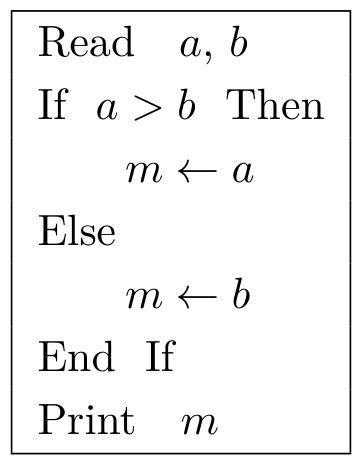
\includegraphics[width=4.3cm]{GaoKao/images/2011/jiangsu/q4_fig1.png}
\end{center}

        \item 从 \(1\)，\(2\)，\(3\)，\(4\) 这四个数中一次随机取两个数，则其中一个数是另一个的两倍的概率是\rule[-0.3ex]{3em}{0.4pt}.

        \item 某老师从星期一到星期五收到信件数分别是 \(10\)，\(6\)，\(8\)，\(5\)，\(6\)，则该组数据的方差 \(s^2=\)\rule[-0.3ex]{3em}{0.4pt}.

        \item 已知 \(\tan\left(x+\frac{\pi}{4}\right)=2\)，则 \(\frac{\tan x}{\tan 2x}\) 的值为\rule[-0.3ex]{3em}{0.4pt}.

        \item 在平面直角坐标系 \(xOy\) 中，过坐标原点的一条直线与函数 \(f(x)=\frac{2}{x}\) 的图象交于 \(P\)，\(Q\) 两点，则线段 \(PQ\) 长的最小值是\rule[-0.3ex]{3em}{0.4pt}.

        \item 函数 \(f(x)=A\sin(\omega x+\varphi)\)（\(A\)，\(\omega\)，\(\varphi\) 是常数，\(A>0\)，\(\omega>0\)）的部分图象如图所示，则 \(f(0)=\)\rule[-0.3ex]{3em}{0.4pt}.

\begin{center}
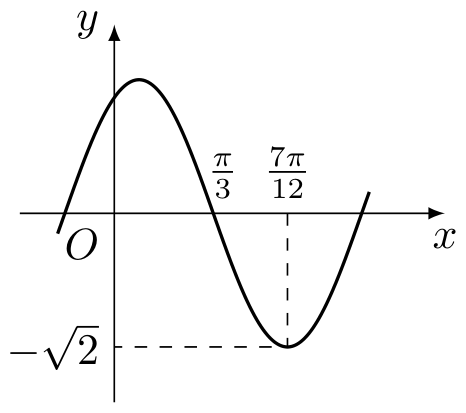
\includegraphics[width=4.8cm]{GaoKao/images/2011/jiangsu/q9_fig1.png}
\end{center}

        \item 已知 \(\bm{e}_1\)，\(\bm{e}_2\) 是夹角为 \(\frac{2\pi}{3}\) 的两个单位向量，\(\bm{a}=\bm{e}_1-2\bm{e}_2\)，\(\bm{b}=k\bm{e}_1+\bm{e}_2\). 若 \(\bm{a}\cdot\bm{b}=0\)，则 \(k\) 的值为\rule[-0.3ex]{3em}{0.4pt}.

        \item 已知实数 \(a\neq 0\)，函数 \(f(x)=\begin{cases}
2x+a, & x<1,\\
-x-2a, & x\geqslant 1.
\end{cases}\)
若 \(f(1-a)=f(1+a)\)，则 \(a\) 的值为\rule[-0.3ex]{3em}{0.4pt}.

        \item 在平面直角坐标系 \(xOy\) 中，已知点 \(P\) 是函数 \(f(x)={\mathrm{e}}^x\) （\(x>0\)）的图象上的动点，该图象在 \(P\) 处的切线 \(l\) 交 \(y\) 轴于点 \(M\). 过点 \(P\) 作 \(l\) 的垂线交 \(y\) 轴于点 \(N\). 设线段 \(MN\) 的中点的纵坐标为 \(t\)，则 \(t\) 的最大值是\rule[-0.3ex]{3em}{0.4pt}.

        \item 设 \(1=a_{1}\leqslant a_{2}\leqslant \cdots \leqslant a_{7}\)，其中 \(a_{1}\)，\(a_{3}\)，\(a_{5}\)，\(a_{7}\) 成公比为 \(q\) 的等比数列，\(a_{2}\)，\(a_{4}\)，\(a_{6}\) 成公差为 \(1\) 的等差数列，则 \(q\) 的最小值是\rule[-0.3ex]{3em}{0.4pt}.

        \item 设集合 \(A=\left\{(x,y)\mid \frac{m}{2}\leqslant (x-2)^2+y^2\leqslant m^2,\ x,y\in\mathbb{R}\right\}\).

集合 \(B=\left\{(x,y)\mid 2m\leqslant x+y\leqslant 2m+1,\ x,y\in\mathbb{R}\right\}\).
若 \(A\cap B\neq\emptyset\)，则实数 \(m\) 的取值范围是\rule[-0.3ex]{3em}{0.4pt}.

    \end{enumerate}

\end{description}

\begin{description}

    \item[二、解答题]

    \begin{enumerate}[leftmargin=5pt]

      \addtocounter{enumi}{+14}

        \item 在 \(\triangle ABC\) 中，角 \(A\)，\(B\)，\(C\) 所对应的边为 \(a\)，\(b\)，\(c\).
\begin{enumerate}
\item 若 \(\sin\left(A+\frac{\pi}{6}\right)=2\cos A\)，求 \(A\) 的值；
\item 若 \(\cos A=\frac{1}{3}\)，\(b=3c\)，求 \(\sin C\) 的值.
\end{enumerate}

        \item 如图，在四棱锥 \(P-ABCD\) 中，平面 \(PAD\perp\) 平面 \(ABCD\)，\(AB=AD\)，\(\angle BAD=60^\circ\)，\(E\)，\(F\) 分别是 \(AP\)，\(AD\) 的中点. 求证：
\begin{enumerate}
\item 直线 \(EF\parallel\) 平面 \(PCD\)；
\item 平面 \(BEF\perp\) 平面 \(PAD\).
\end{enumerate}
\begin{center}
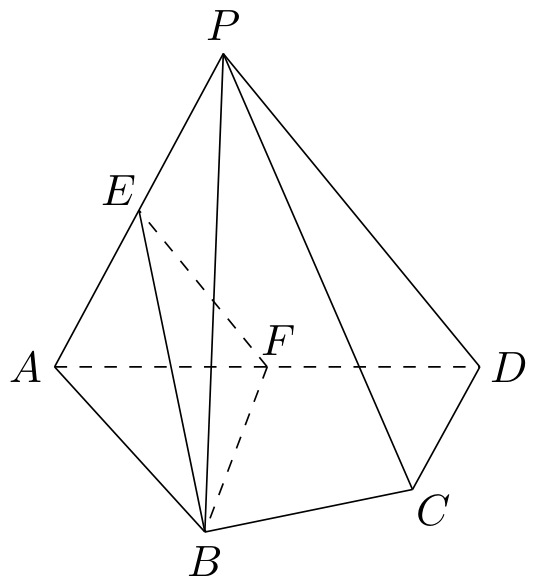
\includegraphics[width=6.7cm]{GaoKao/images/2011/jiangsu/q16_fig1.png}
\end{center}

        \item 请你设计一个包装盒. 如图所示，\(ABCD\) 是边长为 \(60\mathrm{~cm}\) 的正方形硬纸片，切去阴影部分所示的四个全等的等腰直角三角形，再沿虚线折起，使得 \(A\)，\(B\)，\(C\)，\(D\) 四个点重合于图中的点 \(P\)，正好形成一个正四棱柱形状的包装盒，\(E\)，\(F\) 在 \(AB\) 上，是被切去的等腰直角三角形斜边的两个端点. 设 \(AE=FB=x\)（\(\mathrm{cm}\)）.

\begin{enumerate}
\item 若广告商要求包装盒侧面积 \(S\)（\(\mathrm{cm}^2\)）最大，试问 \(x\) 应取何值？
\item 若广告商要求包装盒容积 \(V\)（\(\mathrm{cm}^3\)）最大，试问 \(x\) 应取何值？ 并求出此时包装盒的高与底面边长的比值.
\end{enumerate}
\begin{center}
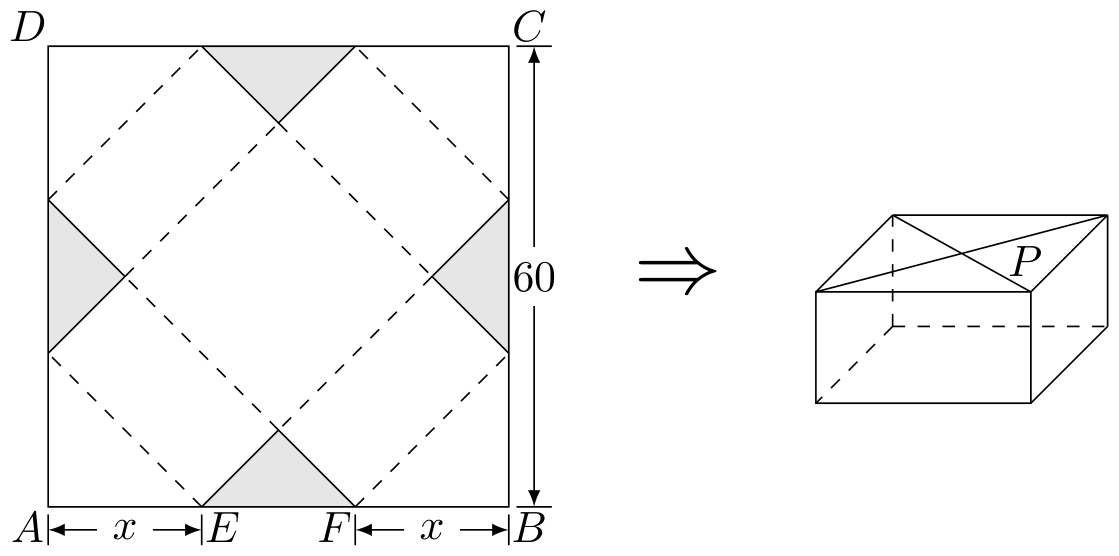
\includegraphics[width=10.9cm]{GaoKao/images/2011/jiangsu/q17_fig1.png}
\end{center}

        \item 如图，在平面直角坐标系 \(xOy\) 中，\(M\)，\(N\) 分别是椭圆 \(\frac{x^2}{4}+\frac{y^2}{2}=1\) 的顶点，过坐标原点的直线交椭圆于 \(P\)，\(A\) 两点，其中点 \(P\) 在第一象限，过 \(P\) 作 \(x\) 轴的垂线，垂足为 \(C\)，连接 \(AC\)，并延长交椭圆于点 \(B\)，设直线 \(PA\) 的斜率为 \(k\).

\begin{enumerate}
\item 当直线 \(PA\) 平分线段 \(MN\) 时，求 \(k\) 的值；
\item 当 \(k=2\) 时，求点 \(P\) 到直线 \(AB\) 的距离 \(d\)；
\item 对任意 \(k>0\)，求证：\(PA\perp PB\).
\end{enumerate}
\begin{center}
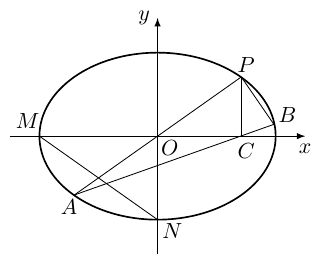
\includegraphics[width=8.0cm]{GaoKao/images/2011/jiangsu/q18_fig1.png}
\end{center}

        \item 已知 \(a\)，\(b\) 是实数，函数 \(f(x)=x^3+ax\)，\(g(x)=x^2+bx\)，\(f'(x)\) 和 \(g'(x)\) 分别是 \(f(x)\)，\(g(x)\) 的导函数，若 \(f'(x)g'(x)\geqslant 0\) 在区间 \(I\) 上恒成立，则称 \(f(x)\) 和 \(g(x)\) 在区间 \(I\) 上单调性一致.

\begin{enumerate}
\item 设 \(a>0\)，若函数 \(f(x)\) 和 \(g(x)\) 在区间 \([-1,+\infty)\) 上单调性一致，求实数 \(b\) 的取值范围；
\item 设 \(a<0\) 且 \(a\neq b\)，若 \(f(x)\) 和 \(g(x)\) 在以 \(a\)，\(b\) 为端点的开区间上单调性一致，求 \(|a-b|\) 的最大值.
\end{enumerate}

        \item 设 \(M\) 为部分正整数组成的集合，数列 \(\{a_{n}\}\) 的首项 \(a_{1}=1\)，前 \(n\) 项和为 \(S_{n}\)，已知对任意整数 \(k\in M\)，当整数 \(n>k\) 时，\(S_{n+k}+S_{n-k}=2(S_{n}+S_{k})\) 都成立.

\begin{enumerate}
\item 设 \(M=\{1\}\)，\(a_{2}=2\)，求 \(a_{5}\) 的值；
\item 设 \(M=\{3,4\}\)，求数列 \(\{a_{n}\}\) 的通项公式.
\end{enumerate}

    \end{enumerate}

\end{description}

\begin{description}

    \item[三、附加题]

    \begin{enumerate}[leftmargin=5pt]

      \addtocounter{enumi}{+20}

        \item [A]
如图，圆 \(O_{1}\) 与圆 \(O_{2}\) 内切于点 \(A\)，其半径分别为 \(r_1\) 与 \(r_2\)（\(r_1>r_2\)），圆 \(O_{1}\) 的弦 \(AB\) 交圆 \(O_{2}\) 于点 \(C\)（\(O_{1}\) 不在 \(AB\) 上），求证：\(AB:AC\) 为定值.

\begin{center}
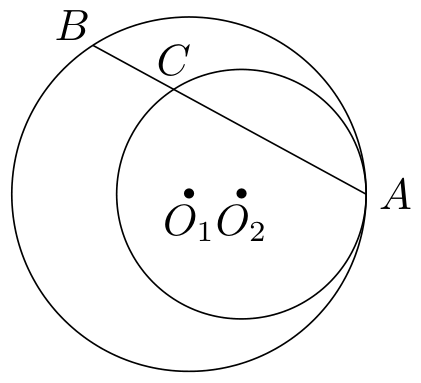
\includegraphics[width=4.9cm]{GaoKao/images/2011/jiangsu/q21_fig1.png}
\end{center}

        \item [B]
已知矩阵 \(A=\begin{bmatrix}1&1\\ 2&1\end{bmatrix}\)，向量 \(\bm{\beta}=\begin{bmatrix}1\\ 2\end{bmatrix}\)，求向量 \(\bm{\alpha}\)，使得 \(A^{2}\bm{\alpha}=\bm{\beta}\).

        \item [C]
在平面直角坐标系 \(xOy\) 中，求过椭圆 \(\begin{cases}
x=5\cos\varphi,\\
y=3\sin\varphi,
\end{cases}\)
（\(\varphi\) 为参数）的右焦点，且与直线 \(\begin{cases}
x=4-2t,\\
y=3-t,
\end{cases}\)
（\(t\) 为参数）平行的直线的普通方程.

        \item [D]
解不等式：\(x+|2x-1|<3\).

        \item 如图，在正四棱柱 \(ABCD-A_{1}B_{1}C_{1}D_{1}\) 中，\(AA_{1}=2\)，\(AB=1\)，点 \(N\) 是 \(BC\) 的中点，点 \(M\) 在 \(CC_{1}\) 上. 设二面角 \(A_{1}-DN-M\) 的大小为 \(\theta\).
\begin{enumerate}
\item 当 \(\theta=90^\circ\) 时，求 \(AM\) 的长；
\item 当 \(\cos\theta=\frac{\sqrt{6}}{6}\) 时，求 \(CM\) 的长.
\end{enumerate}
\begin{center}
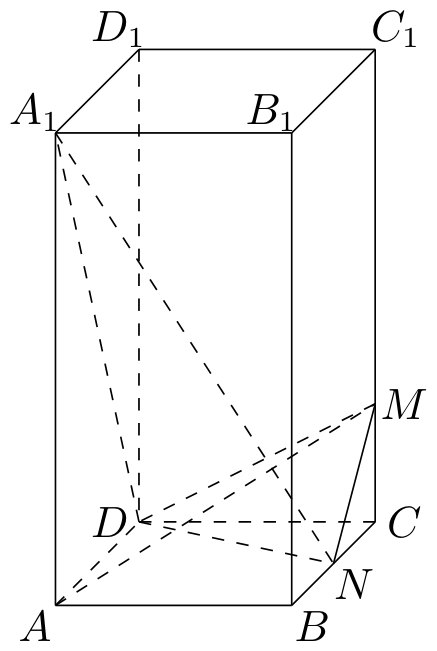
\includegraphics[width=4.4cm]{GaoKao/images/2011/jiangsu/q22_fig1.png}
\end{center}

        \item 设整数 \(n\geqslant 4\)，\(P(a,b)\) 是平面直角坐标系 \(xOy\) 中的点，其中 \(a,b\in\{1,2,3,\dots,n\}\)，\(a>b\).
\begin{enumerate}
\item 记 \(A_{n}\) 为满足 \(a-b=3\) 的点 \(P\) 的个数，求 \(A_{n}\)；
\item 记 \(B_{n}\) 为满足 \(\frac{1}{3}(a-b)\) 是整数的点 \(P\) 的个数，求 \(B_{n}\).
\end{enumerate}

    \end{enumerate}

\end{description}


\subsection{2011年江西卷（理）}\label{gk:2011年江西卷（理）}

\begin{description}

    \item[一、选择题]

    \begin{enumerate}[leftmargin=5pt]

        \item 若 \(z = \frac{1 + 2\i}{\i}\)，则复数 \(z =\)（\quad）

        {\centering\begin{tabular*}{\linewidth}{@{}@{\extracolsep{\fill}}llll@{}}
          \text{A. }\(-2 - \i\)  &  \text{B. }\(-2 + \i\)  &  \text{C. }\(2 - \i\)  &  \text{D. }\(2 + \i\)
        \end{tabular*}\par}

        \item 若集合 \(A = \{x \mid -1 \leqslant 2x + 1 \leqslant 3\}\)，\(B = \left\{x \left| \frac{x - 2}{x} \leqslant 0 \right.\right\}\)，则 \(A \cap B =\)（\quad）

        {\centering\begin{tabular*}{\linewidth}{@{}@{\extracolsep{\fill}}llll@{}}
          \text{A. }\(\{x\mid -1\leqslant x < 0\}\)  &  \text{B. }\(\{x\mid 0 < x\leqslant 1\}\)  &  \text{C. }\(\{x\mid 0\leqslant x\leqslant 2\}\)  &  \text{D. }\(\{x\mid 0\leqslant x\leqslant 1\}\)
        \end{tabular*}\par}

        \item 若 \( f(x) = \frac{1}{\sqrt{\log_{\frac{1}{2}}(2x + 1)}} \)，则 \( f(x) \) 定义域为（\quad）

        {\centering\begin{tabular*}{\linewidth}{@{}@{\extracolsep{\fill}}llll@{}}
          \text{A. }\(\left(-\frac{1}{2},0\right)\)  &  \text{B. }\(\left(-\frac{1}{2},0\right]\)  &  \text{C. }\(\left(-\frac{1}{2}, +\infty\right)\)  &  \text{D. }\((0, +\infty)\)
        \end{tabular*}\par}

        \item 若 \( f(x) = x^2 - 2x - 4\ln x \)，则 \( f'(x) > 0 \) 的解集为（\quad）

        {\centering\begin{tabular*}{\linewidth}{@{}@{\extracolsep{\fill}}llll@{}}
          \text{A. }\((0, +\infty)\)  &  \text{B. }\((-1,0)\cup (2, + \infty)\)  &  \text{C. }\((2, +\infty)\)  &  \text{D. }\((-1,0)\)
        \end{tabular*}\par}

        \item 已知数列 \(\{a_{n}\}\) 的前 \(n\) 项和 \(S_{n}\) 满足： \(S_{n} + S_{m} = S_{n + m}\)，且 \(a_{1} = 1\)，那么 \(a_{10} =\)（\quad）

        {\centering\begin{tabular*}{\linewidth}{@{}@{\extracolsep{\fill}}llll@{}}
          \text{A. }1  &  \text{B. }9  &  \text{C. }10  &  \text{D. }55
        \end{tabular*}\par}

        \item 变量 \(X\) 与 \(Y\) 相对应的一组数据为 \((10, 1)\)，\((11.3, 2)\)，\((11.8, 3)\)，\((12.5, 4)\)，\((13, 5)\)；变量 \(U\) 与 \(V\) 相对应的一组数据为 \((10, 5)\)，\((11.3, 4)\)，\((11.8, 3)\)，\((12.5, 2)\)，\((13, 1)\). \(r_{1}\) 表示变量 \(Y\) 与 \(X\) 之间的线性相关系数；\(r_{2}\) 表示变量 \(V\) 与 \(U\) 之间的线性相关系数，则（\quad）

        {\centering\begin{tabular*}{\linewidth}{@{}@{\extracolsep{\fill}}llll@{}}
          \text{A. }\(r_2 < r_1 < 0\)  &  \text{B. }\(0 < r_2 < r_1\)  &  \text{C. }\(r_2 < 0 < r_1\)  &  \text{D. }\(r_2 = r_1\)
        \end{tabular*}\par}

        \item 观察下列各式： \(5^{5} = 3125\)，\(5^{6} = 15625\)，\(5^{7} = 78125\)，\(\cdots\)，则 \(5^{2011}\) 的末四位数字为（\quad）

        {\centering\begin{tabular*}{\linewidth}{@{}@{\extracolsep{\fill}}llll@{}}
          \text{A. }3125  &  \text{B. }5625  &  \text{C. }0625  &  \text{D. }8125
        \end{tabular*}\par}

        \item 已知 \(\alpha_{1}\)，\(\alpha_{2}\)，\(\alpha_{3}\) 是三个相互平行的平面，平面 \(\alpha_{1}\)，\(\alpha_{2}\) 之间的距离为 \(d_{1}\)，平面 \(\alpha_{2}\)，\(\alpha_{3}\) 之间的距离为 \(d_{2}\). 直线 \(l\) 与 \(\alpha_{1}\)，\(\alpha_{2}\)，\(\alpha_{3}\) 分别交于 \(P_{1}\)，\(P_{2}\)，\(P_{3}\). 那么“\(P_{1}P_{2} = P_{2}P_{3}\)”是“\(d_{1} = d_{2}\)”的（\quad）

        {\centering\begin{tabular*}{\linewidth}{@{}@{\extracolsep{\fill}}llll@{}}
          \text{A. }充分不必要条件  &  \text{B. }必要不充分条件  &  \text{C. }充分必要条件  &  \text{D. }既不充分也不必要条件
        \end{tabular*}\par}

        \item 若曲线 \(C_{1}: x^{2} + y^{2} - 2x = 0\) 与曲线 \(C_{2}: y (y - mx - m) = 0\) 有四个不同的交点，则实数 \(m\) 的取值范围是（\quad）

        {\centering\begin{tabular*}{\linewidth}{@{}@{\extracolsep{\fill}}llll@{}}
          \text{A. }\(\left(-\frac{\sqrt{3}}{3}, \frac{\sqrt{3}}{3}\right)\)  &  \text{B. }\(\left(-\frac{\sqrt{3}}{3}, 0\right) \cup \left(0, \frac{\sqrt{3}}{3}\right)\)  &  \text{C. }\(\left[-\frac{\sqrt{3}}{3}, \frac{\sqrt{3}}{3}\right]\)  &  \text{D. }\(\left(-\infty, -\frac{\sqrt{3}}{3}\right) \cup \left(\frac{\sqrt{3}}{3}, +\infty\right)\)
        \end{tabular*}\par}

        \item 如图，一个直径为 1 的小圆沿着直径为 2 的大圆内壁逆时针方向滚动，\(M\) 和 \(N\) 是小圆的一条固定直径的两个端点. 那么，当小圆这样滚过大圆内壁一周，点 \(M\)，\(N\) 在大圆内所绘出的图形大致是（\quad）

\begin{center}
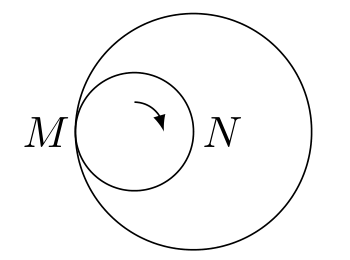
\includegraphics[width=4.8cm]{GaoKao/images/2011/jiangxi_science/q10_fig1.png}
\end{center}

        {\centering\begin{tabular*}{\linewidth}{@{}@{\extracolsep{\fill}}cccc@{}}
          \text{A. }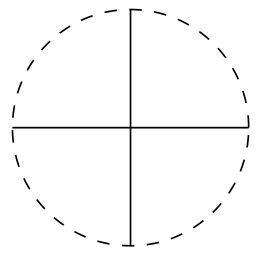
\includegraphics[width=0.15\paperwidth]{GaoKao/images/2011/jiangxi_science/q10_optA.png}  &  \text{B. }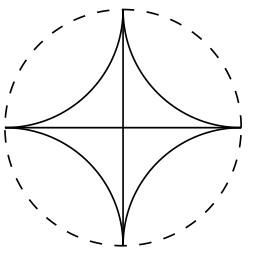
\includegraphics[width=0.15\paperwidth]{GaoKao/images/2011/jiangxi_science/q10_optB.png}  &  \text{C. }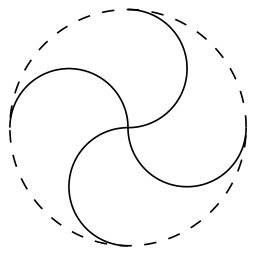
\includegraphics[width=0.15\paperwidth]{GaoKao/images/2011/jiangxi_science/q10_optC.png}  &  \text{D. }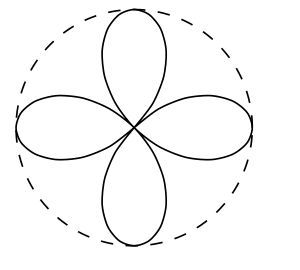
\includegraphics[width=0.15\paperwidth]{GaoKao/images/2011/jiangxi_science/q10_optD.png}
        \end{tabular*}\par}

    \end{enumerate}

\end{description}

\begin{description}

    \item[二、填空题]

    \begin{enumerate}[leftmargin=5pt]

      \addtocounter{enumi}{+10}

        \item 已知 \(|a| = |b| = 2\)，\((a + 2b) \cdot (a - b) = -2\)，则 \(a\) 与 \(b\) 的夹角为\rule[-0.3ex]{3em}{0.4pt}.

        \item 小波通过做游戏的方式来确定周末活动，他随机地往单位圆内投掷一点，若此点到圆心的距离大于 \(\frac{1}{2}\)，则周末去看电影；若此点到圆心的距离小于 \(\frac{1}{4}\)，则去打篮球；否则，在家看书. 则小波周末不在家看书的概率为\rule[-0.3ex]{3em}{0.4pt}.

        \item 下图是某算法程序框图，则程序运行后输出的结果是\rule[-0.3ex]{3em}{0.4pt}.

\begin{center}
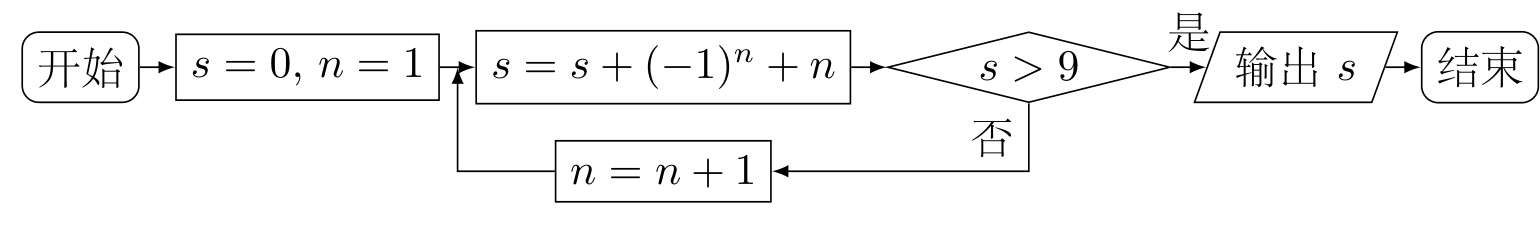
\includegraphics[width=0.96\linewidth]{GaoKao/images/2011/jiangxi_science/q13_fig1.png}
\end{center}

        \item 若椭圆 \(\frac{x^2}{a^2} + \frac{y^2}{b^2} = 1\) 的焦点在 \(x\) 轴上，过点 \(\left(1, \frac{1}{2}\right)\) 作圆 \(x^2 + y^2 = 1\) 的切线. 切点分别为 \(A\)，\(B\)，直线 \(AB\) 恰好经过椭圆的右焦点和上顶点，则椭圆方程是\rule[-0.3ex]{3em}{0.4pt}.

    \end{enumerate}

\end{description}

\begin{description}

    \item[三、选做题]

    \begin{enumerate}[leftmargin=5pt]

      \addtocounter{enumi}{+14}

        \item \textbf{【选修4-4：坐标系与参数方程】}

[A]
若曲线的极坐标方程为 \(\rho = 2 \sin \theta + 4 \cos \theta\)，以极点为原点，极轴为 \(x\) 轴正半轴建立直角坐标系，则该曲线的直角坐标方程为\rule[-0.3ex]{3em}{0.4pt}.

        \item [B]
对于实数 \(x\)，\(y\)，若 \(|x - 1| \leqslant 1\)，\(|y - 2| \leqslant 1\)，则 \(|x - 2y + 1|\) 的最大值为\rule[-0.3ex]{3em}{0.4pt}.

    \end{enumerate}

\end{description}

\begin{description}

    \item[四、解答题]

    \begin{enumerate}[leftmargin=5pt]

      \addtocounter{enumi}{+16}

        \item 某饮料公司招聘一名员工，现对其进行一项测试，以便确定工资级别. 公司准备了两种不同的饮料共 \(8\text{ 杯}\)，其颜色完全相同，并且其中 \(4\text{ 杯}\) 为 A 饮料，另外 \(4\text{ 杯}\) 为 B 饮料，公司要求此员工一一品尝后，从 \(8\text{ 杯}\) 饮料中选出 \(4\text{ 杯}\) A 饮料. 若 \(4\text{ 杯}\) 都选对，则月工资定为 \(3500\text{ 元}\)；若 \(4\text{ 杯}\) 选对 \(3\text{ 杯}\)，则月工资定为 \(2800\text{ 元}\)；否则月工资定为 \(2100\text{ 元}\). 令 \(X\) 表示此人选对 A 饮料的杯数. 假设此人对 A 和 B 两种饮料没有鉴别能力.

\begin{enumerate}
\item 求 \(X\) 的分布列；
\item 求此员工月工资的期望.
\end{enumerate}

        \item 在 \(\triangle ABC\) 中，角 \(A\)，\(B\)，\(C\) 的对边分别是 \(a\)，\(b\)，\(c\)，已知 \(\sin C + \cos C = 1 - \sin \frac{C}{2}\).
\begin{enumerate}
\item 求 \(\sin C\) 的值；
\item 若 \(a^2 + b^2 = 4(a + b) - 8\)，求边 \(c\) 的值.
\end{enumerate}

        \item 已知两个等比数列 \(\{a_{n}\}\)，\(\{b_{n}\}\)，满足 \(a_{1} = a\)（\(a > 0\)），\(b_{1} - a_{1} = 1\)，\(b_{2} - a_{2} = 2\)，\(b_{3} - a_{3} = 3\).
\begin{enumerate}
\item 若 \(a = 1\)，求数列 \(\{a_{n}\}\) 的通项公式；
\item 若数列 \(\{a_{n}\}\) 唯一，求 \(a\) 的值.
\end{enumerate}

        \item 设 \( f(x) = -\frac{1}{3} x^3 + \frac{1}{2} x^2 + 2ax \).
\begin{enumerate}
\item 若 \( f(x) \) 在 \( \left(\frac{2}{3}, +\infty\right) \) 上存在单调递增区间，求 \(a\) 的取值范围；
\item 当 \(0 < a < 2\) 时，\( f(x) \) 在 \([1, 4]\) 上的最小值为 \(-\frac{16}{3}\)，求 \( f(x) \) 在该区间上的最大值.
\end{enumerate}

        \item \(P(x_0, y_0)\)（\(x_0 \neq \pm a\)）是双曲线 \(E: \frac{x^2}{a^2} - \frac{y^2}{b^2} = 1\)（\(a > 0\)，\(b > 0\)）上一点，\(M\)，\(N\) 分别是双曲线 \(E\) 的左，右顶点. 直线 \(PM\)，\(PN\) 的斜率之积为 \(\frac{1}{5}\).
\begin{enumerate}
\item 求双曲线的离心率；
\item 过双曲线 \(E\) 的右焦点且斜率为 1 的直线交双曲线于 \(A\)，\(B\) 两点，\(O\) 为坐标原点，\(C\) 为双曲线上的一点. 满足 \(\overrightarrow{OC} = \lambda \overrightarrow{OA} + \overrightarrow{OB}\)，求 \(\lambda\) 的值.
\end{enumerate}

        \item \begin{enumerate}
    \item 如图，对于任一给定的四面体 \(A_{1}A_{2}A_{3}A_{4}\)，找出依次排列的四个相互平行的平面 \(\alpha_{1}\)，\(\alpha_{2}\)，\(\alpha_{3}\)，\(\alpha_{4}\)，使得 \(A_{i} \in \alpha_{i}\) （\(i = 1\)，\(2\)，\(3\)，\(4\)），且其中每相邻两个平面间的距离都相等；
    \item 给定依次排列的四个相互平行的平面 \(\alpha_{1}\)，\(\alpha_{2}\)，\(\alpha_{3}\)，\(\alpha_{4}\)，其中每相邻两个平面间的距离都为 1，若一个正四面体 \(A_{1}A_{2}A_{3}A_{4}\) 的四个顶点满足： \(A_{i} \in \alpha_{i}\) （\(i = 1\)，\(2\)，\(3\)，\(4\)），求该正四面体 \(A_{1}A_{2}A_{3}A_{4}\) 的体积.
\end{enumerate}

\begin{center}
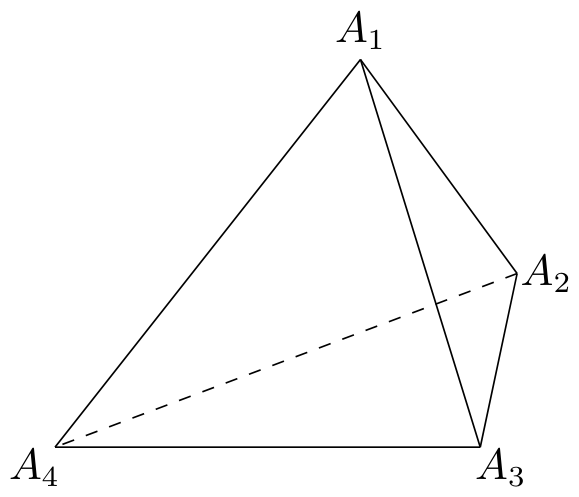
\includegraphics[width=5.6cm]{GaoKao/images/2011/jiangxi_science/q21_fig1.png}
\end{center}

    \end{enumerate}

\end{description}


\subsection{2011年江西卷（文）}\label{gk:2011年江西卷（文）}

\begin{description}

    \item[一、选择题]

    \begin{enumerate}[leftmargin=5pt]

        \item 若 \((x - \i)\i = y + 2\i\)，\(x\)，\(y \in \mathbb{R}\)，则复数 \(x + y\i =\)（\quad）

        {\centering\begin{tabular*}{\linewidth}{@{}@{\extracolsep{\fill}}llll@{}}
          \text{A. }\(-2 + \i\)  &  \text{B. }\(2 + \i\)  &  \text{C. }\(1 - 2\i\)  &  \text{D. }\(1 + 2\i\)
        \end{tabular*}\par}

        \item 若全集 \(U = \{1, 2, 3, 4, 5, 6\}\)，\(M = \{2, 3\}\)，\(N = \{1, 4\}\)，则集合 \(\{5, 6\}\) 等于（\quad）

        {\centering\begin{tabular*}{\linewidth}{@{}@{\extracolsep{\fill}}llll@{}}
          \text{A. }\(M \cup N\)  &  \text{B. }\(M \cap N\)  &  \text{C. }\((\complement_U M) \cup (\complement_U N)\)  &  \text{D. }\((\complement_U M) \cap (\complement_U N)\)
        \end{tabular*}\par}

        \item 若 \( f(x) = \frac{1}{\log_{\frac{1}{2}}(2x + 1)} \)，则 \( f(x) \) 的定义域为（\quad）

        {\centering\begin{tabular*}{\linewidth}{@{}@{\extracolsep{\fill}}llll@{}}
          \text{A. }\(\left(-\frac{1}{2}, 0\right)\)  &  \text{B. }\(\left(-\frac{1}{2}, +\infty\right)\)  &  \text{C. }\(\left(-\frac{1}{2}, 0\right) \cup (0, +\infty)\)  &  \text{D. }\(\left(-\frac{1}{2}, 2\right)\)
        \end{tabular*}\par}

        \item 曲线 \( y = {\mathrm{e}}^{x} \) 在点 \( A(0,1) \) 处的切线斜率为（\quad）

        {\centering\begin{tabular*}{\linewidth}{@{}@{\extracolsep{\fill}}llll@{}}
          \text{A. }\(1\)  &  \text{B. }\(2\)  &  \text{C. }\({\mathrm{e}}\)  &  \text{D. }\(\frac{1}{{\mathrm{e}}}\)
        \end{tabular*}\par}

        \item 设 \(\{a_{n}\}\) 为等差数列，公差 \(d = -2\)，\(S_{n}\) 为其前 \(n\) 项和. 若 \(S_{10} = S_{11}\)，则 \(a_{1} =\)（\quad）

        {\centering\begin{tabular*}{\linewidth}{@{}@{\extracolsep{\fill}}llll@{}}
          \text{A. }\(18\)  &  \text{B. }\(20\)  &  \text{C. }\(22\)  &  \text{D. }\(24\)
        \end{tabular*}\par}

        \item 观察下列各式： \(7^{2} = 49\)，\(7^{3} = 343\)，\(7^{4} = 2401\)，\(\cdots\)，则 \(7^{2011}\) 的末两位数字为（\quad）

        {\centering\begin{tabular*}{\linewidth}{@{}@{\extracolsep{\fill}}llll@{}}
          \text{A. }\(01\)  &  \text{B. }\(43\)  &  \text{C. }\(07\)  &  \text{D. }\(49\)
        \end{tabular*}\par}

        \item 为了普及环保知识，增强环保意识，某大学随机抽取 30 名学生参加环保知识测试，得分 （十分制） 如图所示，假设得分值的中位数为 \(m_{e}\)，众数为 \(m_{o}\)，平均值为 \(\overline{x}\)，则（\quad）

\begin{center}
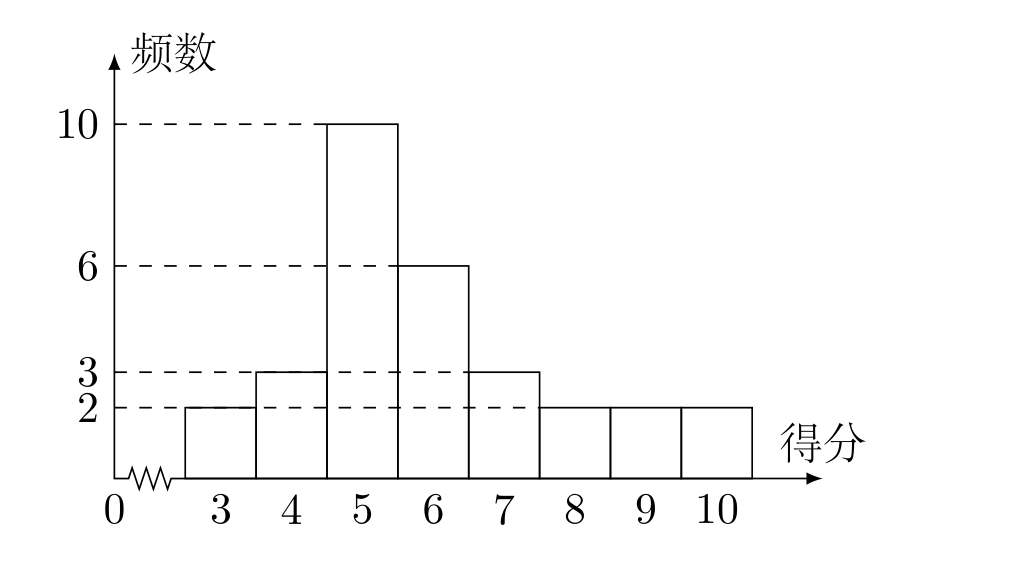
\includegraphics[width=0.72\linewidth]{GaoKao/images/2011/jiangxi_liberal/q7_fig1.png}
\end{center}

        {\centering\begin{tabular*}{\linewidth}{@{}@{\extracolsep{\fill}}llll@{}}
          \text{A. }\(m_{e} = m_{o} = \overline{x}\)  &  \text{B. }\(m_{e} = m_{o} < \overline{x}\)  &  \text{C. }\(m_{e} < m_{o} < \overline{x}\)  &  \text{D. }\(m_{o} < m_{e} < \overline{x}\)
        \end{tabular*}\par}

        \item 为了解儿子身高与其父亲身高的关系，随机抽取 5 对父子的身高数据如下：
\begin{center}
\renewcommand{\arraystretch}{1.1}
\begin{tabular}{c|ccccc}
父亲身高 \(x(\mathrm{cm})\) & 174 & 176 & 176 & 176 & 178 \\
\hline
儿子身高 \(y(\mathrm{cm})\) & 175 & 175 & 176 & 177 & 177
\end{tabular}
\end{center}
则 \(y\) 对 \(x\) 的线性回归方程为（\quad）

        {\centering\begin{tabular*}{\linewidth}{@{}@{\extracolsep{\fill}}llll@{}}
          \text{A. }\(y = x - 1\)  &  \text{B. }\(y = x + 1\)  &  \text{C. }\(y = 88 + \frac{1}{2} x\)  &  \text{D. }\(y = 176\)
        \end{tabular*}\par}

        \item 将长方体截去一个四棱锥，得到的几何体如图所示，则该几何体的左视图为（\quad）

\begin{center}
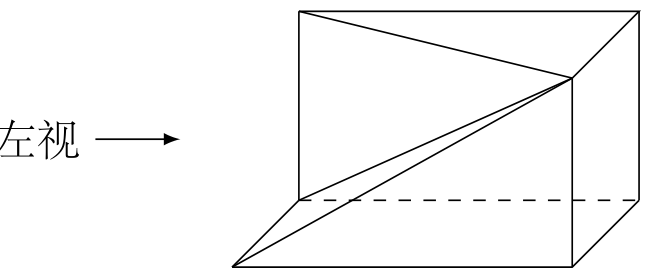
\includegraphics[width=5.9cm]{GaoKao/images/2011/jiangxi_liberal/q9_fig1.png}
\end{center}

        {\centering\begin{tabular*}{\linewidth}{@{}@{\extracolsep{\fill}}cccc@{}}
          \text{A. }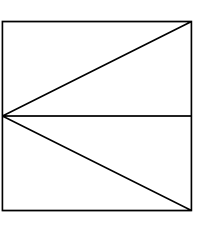
\includegraphics[width=0.15\paperwidth]{GaoKao/images/2011/jiangxi_liberal/q9_choiceA.png}  &  \text{B. }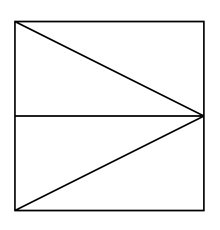
\includegraphics[width=0.15\paperwidth]{GaoKao/images/2011/jiangxi_liberal/q9_choiceB.png}  &  \text{C. }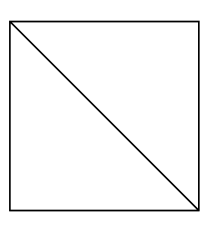
\includegraphics[width=0.15\paperwidth]{GaoKao/images/2011/jiangxi_liberal/q9_choiceC.png}  &  \text{D. }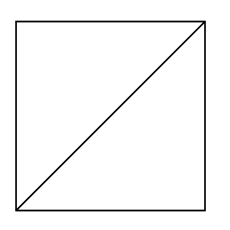
\includegraphics[width=0.15\paperwidth]{GaoKao/images/2011/jiangxi_liberal/q9_choiceD.png}
        \end{tabular*}\par}

        \item 如图，一个“凸轮”放置于直角坐标系 \(x\) 轴上方，其“底端”落在原点 \(O\) 处，一顶点及中心 \(M\) 在 \(y\) 轴正半轴上，它的外围由以正三角形的顶点为圆心，以正三角形的边长为半径的三段等弧组成. 今使“凸轮”沿 \(x\) 轴正向滚动前进，在滚动过程中“凸轮”每时每刻都有一个“最高点”，其中心也在不断移动位置. 则在“凸轮”滚动一周的过程中，将其“最高点”和“中心点”所形成的图形按上，下放置，应大致为（\quad）

\begin{center}
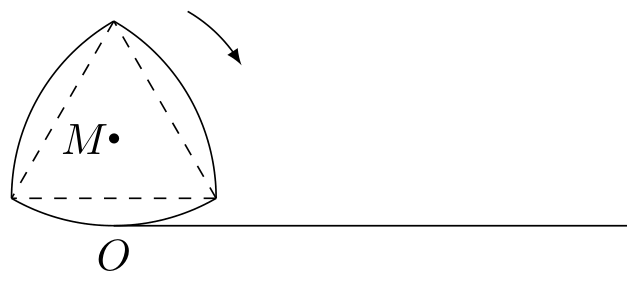
\includegraphics[width=5.5cm]{GaoKao/images/2011/jiangxi_liberal/q10_fig1.png}
\end{center}

        {\centering\begin{tabular*}{\linewidth}{@{}@{\extracolsep{\fill}}cccc@{}}
          \text{A. }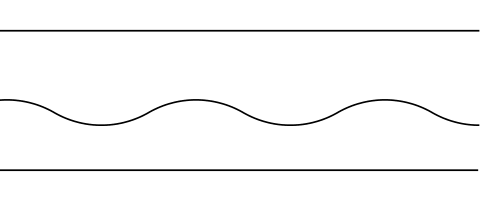
\includegraphics[width=0.15\paperwidth]{GaoKao/images/2011/jiangxi_liberal/q10_choiceA.png}  &  \text{B. }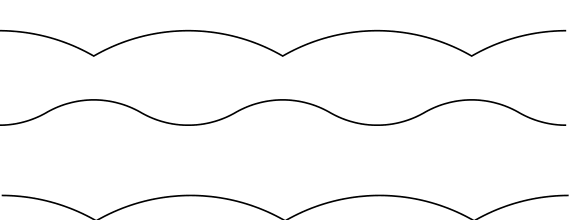
\includegraphics[width=0.15\paperwidth]{GaoKao/images/2011/jiangxi_liberal/q10_choiceB.png}  &  \text{C. }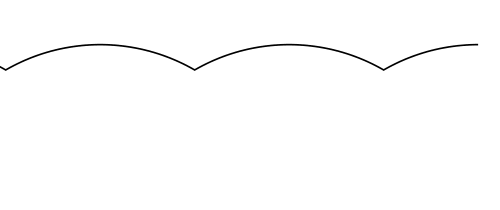
\includegraphics[width=0.15\paperwidth]{GaoKao/images/2011/jiangxi_liberal/q10_choiceC.png}  &  \text{D. }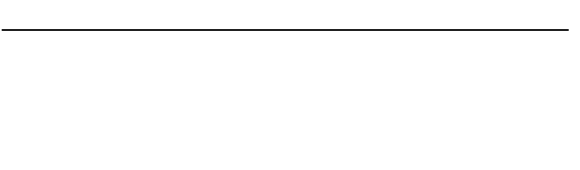
\includegraphics[width=0.15\paperwidth]{GaoKao/images/2011/jiangxi_liberal/q10_choiceD.png}
        \end{tabular*}\par}

    \end{enumerate}

\end{description}

\begin{description}

    \item[二、填空题]

    \begin{enumerate}[leftmargin=5pt]

      \addtocounter{enumi}{+10}

        \item 已知两个单位向量 \(e_{1}\)，\(e_{2}\) 的夹角为 \( \frac{\pi}{3} \)，若向量 \(b_{1} = e_{1} - 2e_{2}\)，\(b_{2} = 3e_{1} + 4e_{2}\)，则 \( b_{1} \cdot b_{2} = \)\rule[-0.3ex]{3em}{0.4pt}.

        \item 若双曲线 \(\frac{y^2}{16} - \frac{x^2}{m} = 1\) 的离心率 \(e = 2\)，则 \(m = \)\rule[-0.3ex]{3em}{0.4pt}.

        \item 下图是某算法程序框图，则程序运行后输出的结果是\rule[-0.3ex]{3em}{0.4pt}.

\begin{center}
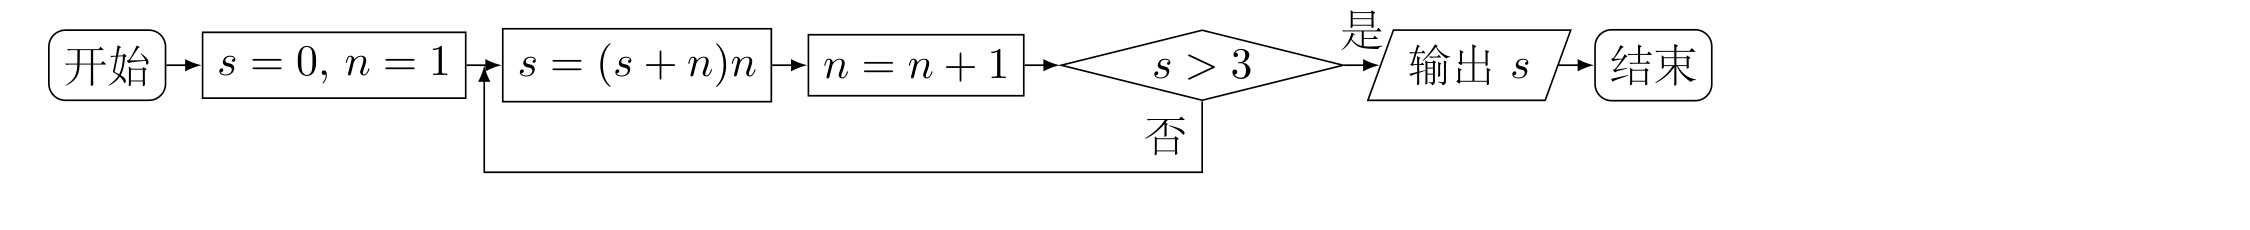
\includegraphics[width=0.96\linewidth]{GaoKao/images/2011/jiangxi_liberal/q13_fig1.png}
\end{center}

        \item 已知角 \(\theta\) 的顶点为坐标原点，始边为 \(x\) 轴的正半轴. 若 \(P(4, y)\) 是角 \(\theta\) 终边上一点，且 \(\sin \theta = -\frac{2\sqrt{5}}{5}\)，则 \(y =\rule[-0.3ex]{3em}{0.4pt}\).

        \item 对于 \(x \in \mathbb{R}\)，不等式 \(|x + 10| - |x - 2| \geqslant 8\) 的解集为\rule[-0.3ex]{3em}{0.4pt}.

    \end{enumerate}

\end{description}

\begin{description}

    \item[三、解答题]

    \begin{enumerate}[leftmargin=5pt]

      \addtocounter{enumi}{+15}

        \item 某饮料公司对一名员工进行测试以便确定其考评级别. 公司准备了两种不同的饮料共5杯，其颜色完全相同，并且其中3杯为A饮料，另外2杯为B饮料，公司要求此员工一一品尝后，从5杯饮料中选出3杯A饮料. 若 该员工3杯都选对，则评为优秀；若3杯选对2杯，则评为良好；否则评为及格. 假设此人对 \(A\) 和 \(B\) 两种饮料没有鉴别能力.
\begin{enumerate}
\item 求此人被评为优秀的概率；
\item 求此人被评为良好及以上的概率.
\end{enumerate}

        \item 在 \(\triangle ABC\) 中，\(A\)，\(B\)，\(C\) 的对边分别是 \(a\)，\(b\)，\(c\). 已知 \(3a \cos A = c \cos B + b \cos C\).
\begin{enumerate}
\item 求 \( \cos A \) 的值；
\item 若 \(a = 1\)，\(\cos B + \cos C = \frac{2\sqrt{3}}{3}\)，求边 \(c\) 的值.
\end{enumerate}

        \item 如图，在 \(\triangle ABC\) 中，\(\angle B = \frac{\pi}{2}\)，\(AB = BC = 2\). \(P\) 为 \(AB\) 边上动一点，\(PD \parallel BC\) 交 \(AC\) 于点 \(D\)，现将 \(\triangle PDA\) 沿 \(PD\) 翻折至 \(\triangle PDA'\)，使平面 \(PDA' \perp\) 平面 \(PBCD\).
\begin{enumerate}
\item 当棱锥 \(A' - PBCD\) 的体积最大时，求 \(PA\) 的长；
\item 若点 \(P\) 为 \(AB\) 的中点，\(E\) 为 \(A'C\) 的中点，求证： \(A'B \perp DE\).
\end{enumerate}

\begin{center}
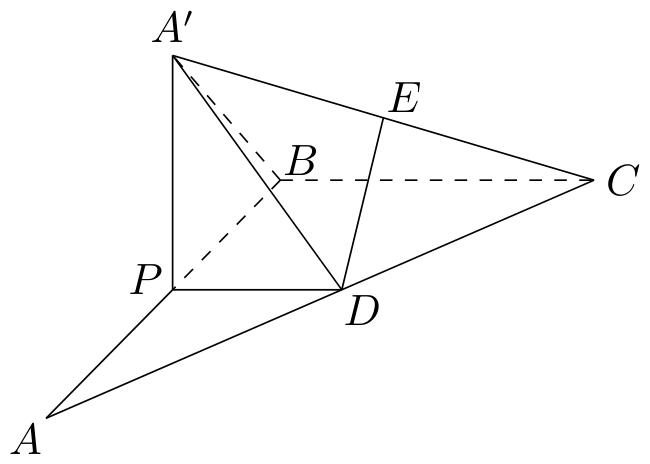
\includegraphics[width=6.4cm]{GaoKao/images/2011/jiangxi_liberal/q18_fig1.png}
\end{center}

        \item 已知过抛物线 \( y^{2} = 2px \) （\( p > 0 \)） 的焦点，斜率为 \( 2\sqrt{2} \) 的直线交抛物线于 \( A(x_{1}, y_{1}) \)，\( B(x_{2}, y_{2}) \) （\( x_{1} < x_{2} \)） 两点，且 \( |AB| = 9 \).
\begin{enumerate}
\item 求该抛物线的方程；
\item O 为坐标原点，C 为抛物线上一点. 若 \( \overrightarrow{OC} = \overrightarrow{OA} + \lambda \overrightarrow{OB} \)，求 \( \lambda \) 的值.
\end{enumerate}

        \item 设 \( f(x) = \frac{1}{3} x^3 + mx^2 + nx \).
\begin{enumerate}
\item 如果 \( g(x) = f'(x) - 2x - 3 \) 在 \( x = -2 \) 处取得最小值 \(-5\)，求 \( f(x) \) 的解析式；
\item 如果 \(m + n < 10\) （\(m\)，\(n \in \mathbf{N}_+\)），\(f(x)\) 的单调递减区间的长度是正整数，试求 \(m\) 和 \(n\) 的值. （注：区间 \((a, b)\) 的长度为 \(b - a\)）
\end{enumerate}

        \item \begin{enumerate}
\item 已知两个等比数列 \(\{a_{n}\}\)，\(\{b_{n}\}\)，满足 \(a_{1} = a\)（\(a > 0\)），\(b_{1} - a_{1} = 1\)，\(b_{2} - a_{2} = 2\)，\(b_{3} - a_{3} = 3\)，若数列 \(\{a_{n}\}\) 唯一，求 \(a\) 的值；
\item 是否存在两个等比数列 \(\{a_{n}\}\)，\(\{b_{n}\}\)，使得 \(b_{1} - a_{1}\)，\(b_{2} - a_{2}\)，\(b_{3} - a_{3}\)，\(b_{4} - a_{4}\) 成公差不为 0 的等差数列？ 若存在，求 \(\{a_{n}\}\)，\(\{b_{n}\}\) 的通项公式；若不存在，说明理由.
\end{enumerate}

    \end{enumerate}

\end{description}


\subsection{2011年辽宁卷（理）}\label{gk:2011年辽宁卷（理）}

\begin{description}

    \item[一、选择题]

    \begin{enumerate}[leftmargin=5pt]

        \item 若 \(a\) 为正实数，\(\i\) 为虚数单位，\(\left|\frac{a + \i}{\i}\right| = 2\)，则 \(a =\)（\quad）

        {\centering\begin{tabular*}{\linewidth}{@{}@{\extracolsep{\fill}}llll@{}}
          \text{A. }2  &  \text{B. }\(\sqrt{3}\)  &  \text{C. }\(\sqrt{2}\)  &  \text{D. }1
        \end{tabular*}\par}

        \item 已知 \(M\)，\(N\) 为集合 \(I\) 的非空真子集，且 \(M\)，\(N\) 不相等，若 \(N \cap \complement_I M = \varnothing\)，则 \(M \cup N =\)（\quad）

        {\centering\begin{tabular*}{\linewidth}{@{}@{\extracolsep{\fill}}llll@{}}
          \text{A. }M  &  \text{B. }N  &  \text{C. }I  &  \text{D. }\(\varnothing\)
        \end{tabular*}\par}

        \item 已知 \(F\) 是抛物线 \(y^{2} = x\) 的焦点，\(A\)，\(B\) 是该抛物线上的两点，\(|AF| + |BF| = 3\)，则线段 \(AB\) 的中点到 \(y\) 轴的距离为（\quad）

        {\centering\begin{tabular*}{\linewidth}{@{}@{\extracolsep{\fill}}llll@{}}
          \text{A. }\( \frac{3}{4} \)  &  \text{B. }1  &  \text{C. }\( \frac{5}{4} \)  &  \text{D. }\( \frac{7}{4} \)
        \end{tabular*}\par}

        \item \(\triangle ABC\) 的三个内角 \(A\)，\(B\)，\(C\) 所对的边分别为 \(a\)，\(b\)，\(c\)，并且有 \(a \sin A \sin B + b \cos^2 A = \sqrt{2} a\)，则 \(\frac{b}{a} =\)（\quad）

        {\centering\begin{tabular*}{\linewidth}{@{}@{\extracolsep{\fill}}llll@{}}
          \text{A. }\(2 \sqrt{3}\)  &  \text{B. }\(2 \sqrt{2}\)  &  \text{C. }\(\sqrt{3}\)  &  \text{D. }\(\sqrt{2}\)
        \end{tabular*}\par}

        \item 从 1， 2， 3， 4， 5 中任取 2 个不同的数，事件 \(A =\) “取到的 2 个数之和为偶数”，事件 \(B =\) “取到的 2 个数均为偶数”，则 \( P(B \mid A) = \)（\quad）

        {\centering\begin{tabular*}{\linewidth}{@{}@{\extracolsep{\fill}}llll@{}}
          \text{A. }\(\frac{1}{8}\)  &  \text{B. }\(\frac{1}{4}\)  &  \text{C. }\(\frac{2}{5}\)  &  \text{D. }\(\frac{1}{2}\)
        \end{tabular*}\par}

        \item 执行下面的程序框图，如果输入的 \(n\) 是 4，则输出的 \(p\) 是（\quad）

\begin{center}
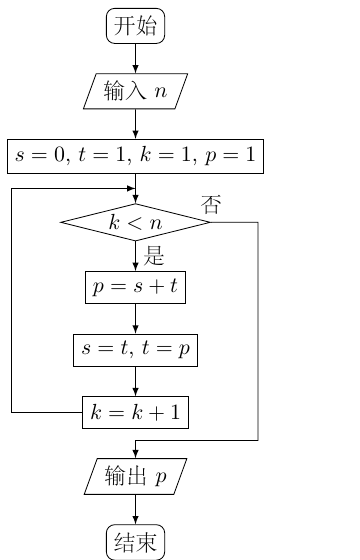
\includegraphics[width=0.42\linewidth]{GaoKao/images/2011/liaoning_science/q6_fig1.png}
\end{center}

        {\centering\begin{tabular*}{\linewidth}{@{}@{\extracolsep{\fill}}llll@{}}
          \text{A. }8  &  \text{B. }5  &  \text{C. }3  &  \text{D. }2
        \end{tabular*}\par}

        \item 设 \(\sin \left(\frac{\pi}{4} + \theta\right) = \frac{1}{3}\)，则 \(\sin 2\theta =\)（\quad）

        {\centering\begin{tabular*}{\linewidth}{@{}@{\extracolsep{\fill}}llll@{}}
          \text{A. }\(-\frac{7}{9}\)  &  \text{B. }\(-\frac{1}{9}\)  &  \text{C. }\( \frac{1}{9} \)  &  \text{D. }\( \frac{7}{9} \)
        \end{tabular*}\par}

        \item 如图，四棱锥 \(S - ABCD\) 的底面为正方形，\(SD \perp\) 底面 \(ABCD\)，则下列结论中不正确的是（\quad）

\begin{center}
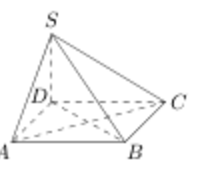
\includegraphics[width=4.1cm]{GaoKao/images/2011/liaoning_science/q8_fig1.png}
\end{center}

        {\centering\begin{tabular*}{\linewidth}{@{}@{\extracolsep{\fill}}llll@{}}
          \text{A. }\(AC \perp SB\)  &  \text{B. }\(AB \parallel\) 平面 \(SCD\)  &  \text{C. }\(SA\) 与平面 \(SBD\) 所成的角等于 \(SC\) 与平面 \(SBD\) 所成的角  &  \text{D. }\(AB\) 与 \(SC\) 所成的角等于 \(DC\) 与 \(SA\) 所成的角
        \end{tabular*}\par}

        \item 设函数 \( f(x) = \begin{cases}
2^{1 - x}, & x \leqslant 1,\\
1 - \log_2 x, & x > 1,
\end{cases} \) 则满足 \( f(x) \leqslant 2 \) 的 \( x \) 取值范围是（\quad）

        {\centering\begin{tabular*}{\linewidth}{@{}@{\extracolsep{\fill}}llll@{}}
          \text{A. }\([-1, 2]\)  &  \text{B. }\([0,2]\)  &  \text{C. }\([1, +\infty)\)  &  \text{D. }\([0, +\infty)\)
        \end{tabular*}\par}

        \item 若 \(a\)，\(b\)，\(c\) 均为单位向量，且 \(a \cdot b = 0\)，\((a - c) \cdot (b - c) \leqslant 0\)，则 \(\lvert a + b - c \rvert\) 的最大值为（\quad）

        {\centering\begin{tabular*}{\linewidth}{@{}@{\extracolsep{\fill}}llll@{}}
          \text{A. }\(\sqrt{2} - 1\)  &  \text{B. }1  &  \text{C. }\(\sqrt{2}\)  &  \text{D. }2
        \end{tabular*}\par}

        \item 函数 \( f(x) \) 的定义域为 \( \mathbb{R} \)，\( f(-1) = 2 \)，对任意 \( x \in \mathbb{R} \)，\( f'(x) > 2 \)，则 \( f(x) > 2x + 4 \) 的解集为（\quad）

        {\centering\begin{tabular*}{\linewidth}{@{}@{\extracolsep{\fill}}llll@{}}
          \text{A. }\((-1, 1)\)  &  \text{B. }\((-1, +\infty)\)  &  \text{C. }\((- \infty, -1)\)  &  \text{D. }\((-\infty, +\infty)\)
        \end{tabular*}\par}

        \item 已知球的直径 \(SC = 4\)，\(A\)，\(B\) 是该球球面上的两点，\(AB = \sqrt{3}\)，\(\angle ASC = \angle BSC = 30^\circ\)，则棱锥 \(S - ABC\) 的体积为（\quad）

        {\centering\begin{tabular*}{\linewidth}{@{}@{\extracolsep{\fill}}llll@{}}
          \text{A. }\(3\sqrt{3}\)  &  \text{B. }\(2\sqrt{3}\)  &  \text{C. }\(\sqrt{3}\)  &  \text{D. }1
        \end{tabular*}\par}

    \end{enumerate}

\end{description}

\begin{description}

    \item[二、填空题]

    \begin{enumerate}[leftmargin=5pt]

      \addtocounter{enumi}{+12}

        \item 已知点 \((2,3)\) 在双曲线 \(C: \frac{x^2}{a^2} - \frac{y^2}{b^2} = 1 \) （\(a > 0, b > 0\)）上，\(C\) 的焦距为 4，则它的离心率为\rule[-0.3ex]{3em}{0.4pt}.

        \item 调查了某地若干户家庭的年收入 \(x\) （单位：万元） 和年饮食支出 \(y\) （单位：万元），调查显示年收入 \(x\) 与年饮食支出 \(y\) 具有线性相关关系. 并由调查数据得到 \(y\) 对 \(x\) 的回归直线方程： \(\hat{y} = 0.254x + 0.321\). 由回归直线方程可知，家庭收入每增加 1 万元，年饮食支出平均增加\rule[-0.3ex]{3em}{0.4pt} 万元.

        \item 一个正三棱柱的侧棱长和底面边长相等，体积为 \(2 \sqrt{3}\)，它的三视图中的俯视图如图所示，左视图是一个矩形，则这个矩形的面积是\rule[-0.3ex]{3em}{0.4pt}

\begin{center}
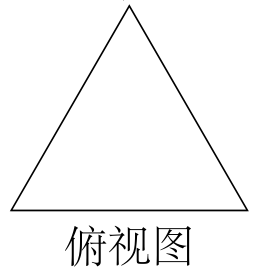
\includegraphics[width=2.5cm]{GaoKao/images/2011/liaoning_science/q15_fig1.png}
\end{center}

        \item 已知函数 \( f(x) = A \tan (\omega x + \varphi) \)（\( \omega > 0, |\varphi| < \frac{\pi}{2} \)），\( y = f(x) \) 的部分图象如图，则 \( f\left(\frac{\pi}{24}\right) = \)\rule[-0.3ex]{3em}{0.4pt}.

\begin{center}
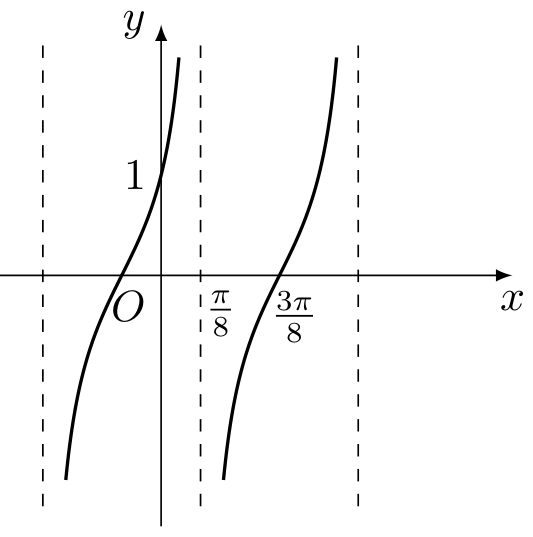
\includegraphics[width=7.6cm]{GaoKao/images/2011/liaoning_science/q16_fig1.png}
\end{center}

    \end{enumerate}

\end{description}

\begin{description}

    \item[三、解答题]

    \begin{enumerate}[leftmargin=5pt]

      \addtocounter{enumi}{+16}

        \item 已知等差数列 \(\{a_{n}\}\) 满足 \(a_{2} = 0\)，\(a_{6} + a_{8} = -10\).
\begin{enumerate}
\item 求数列 \( \{a_{n}\} \) 的通项公式；
\item 求数列 \( \left\{\frac{a_{n}}{2^{n-1}}\right\} \) 的前 \(n\) 项和.
\end{enumerate}

        \item 如图，四边形 \(ABCD\) 为正方形，\(PD \perp\) 平面 \(ABCD\)，\(PD \parallel QA\)，\(QA = AB = \frac{1}{2} PD\).
\begin{enumerate}
\item 证明：平面 \(PQC \perp\) 平面 \(DCQ\)；
\item 求二面角 \(Q - BP - C\) 的余弦值.
\end{enumerate}

\begin{center}
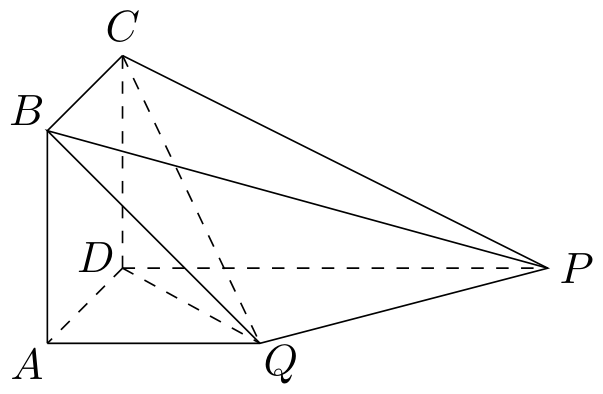
\includegraphics[width=7.2cm]{GaoKao/images/2011/liaoning_science/q18_fig1.png}
\end{center}

        \item 某农场计划种植某种新作物，为此对这种作物的两个品种（分别称为品种甲和品种乙）进行田间试验，选取两大块地. 每大块地分成 \(n\) 小块地. 在总共 \(2n\) 小块地中，随机选 \(n\) 小块地种植品种甲，另外 \(n\) 小块地种植品种乙.
\begin{enumerate}
\item 假设 \(n = 4\)，在第一大块地中，种植品种甲的小块地的数目记为 \(X\)，求 \(X\) 的分布列和数学期望.
\item 试验时每大块地分成 \(8\) 小块，即 \(n = 8\)，试验结束后得到品种甲和品种乙在各小块地上的每公顷产量 （单位： \(\mathrm{kg/hm^2}\)）如下表：
\begin{center}
\begin{tabular}{c|cccccccc}
\hline
品种甲 & 403 & 397 & 390 & 404 & 388 & 400 & 412 & 406 \\
\hline
品种乙 & 419 & 403 & 412 & 418 & 408 & 423 & 400 & 413 \\
\hline
\end{tabular}
\end{center}
分别求品种甲和品种乙每公顷产量的样本平均数和样本方差；根据试验结果，你应该种植哪一品种？

附：样本数据 \(x_{1}\)，\(x_{2}\)，\(\cdots\)，\(x_{n}\) 的样本方差 \(s^{2} = \frac{1}{n}[(x_{1} - \overline{x})^{2} + (x_{2} - \overline{x})^{2} + \cdots + (x_{n} - \overline{x})^{2}]\)，其中 \(\overline{x}\) 为样本平均数.
\end{enumerate}

        \item 已知函数 \( f(x) = \ln x - ax^2 + (2 - a)x \).
\begin{enumerate}
\item 讨论 \(f(x)\) 的单调性；
\item 设 \(a > 0\)，证明：当 \(0 < x < \frac{1}{a}\) 时，\(f\left(\frac{1}{a} + x\right) > f\left(\frac{1}{a} - x\right)\)；
\item 若函数 \( y = f(x) \) 的图象与 \( x \) 轴交于 \(A\)，\(B\) 两点，线段 \(AB\) 中点的横坐标为 \( x_0 \)，证明：\( f'(x_0) < 0 \).
\end{enumerate}

        \item 如图，已知椭圆 \(C_1\) 的中心在原点 \(O\)，长轴左，右端点 \(M\)，\(N\) 在 \(x\) 轴上，椭圆 \(C_2\) 的短轴为 \(MN\)，且 \(C_1\)，\(C_2\) 的离心率都为 \(e\). 直线 \(l \perp MN\)，\(l\) 与 \(C_1\) 交于两点，与 \(C_2\) 交于两点，这四点按纵坐标从大到小依次为 \(A\)，\(B\)，\(C\)，\(D\).
\begin{enumerate}
\item 设 \(e = \frac{1}{2}\)，求 \(|BC|\) 与 \(|AD|\) 的比值.
\item 当 \(e\) 变化时，是否存在直线 \(l\)，使得 \(BO \parallel AN\)，并说明理由.
\end{enumerate}

\begin{center}
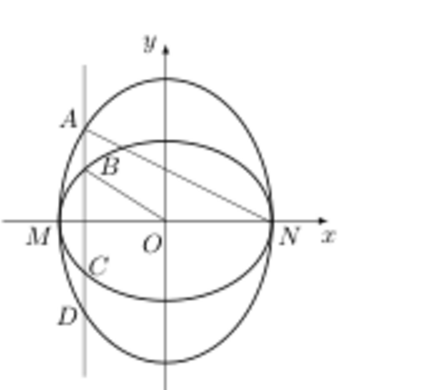
\includegraphics[width=6.0cm]{GaoKao/images/2011/liaoning_science/q20_fig1.png}
\end{center}

    \end{enumerate}

\end{description}

\begin{description}

    \item[四、选考题]

    \begin{enumerate}[leftmargin=5pt]

      \addtocounter{enumi}{+21}

        \item \textbf{【选修4-1：几何证明选讲】}

如图，\(A\)，\(B\)，\(C\)，\(D\) 四点在同一圆上，\(AD\) 的延长线与 \(BC\) 的延长线交于 \(E\) 点，且 \(EC = ED\).
\begin{enumerate}
\item 证明： \(CD \parallel AB\)；
\item 延长 \(CD\) 到 \(F\)，延长 \(DC\) 到 \(G\)，使得 \(EF = EG\)，证明： \(A\)，\(B\)，\(G\)，\(F\) 四点共圆.
\end{enumerate}

\begin{center}
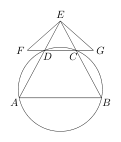
\includegraphics[width=5.6cm]{GaoKao/images/2011/liaoning_science/q22_fig1.png}
\end{center}

        \item \textbf{【选修4-4：坐标系与参数方程】}

在平面直角坐标系 \(xOy\) 中，曲线 \(C_1\) 的参数方程为 \(\begin{cases}
x = \cos \varphi,\\
y = \sin \varphi.
\end{cases}\) （\(\varphi\) 为参数）. 曲线 \(C_2\) 的参数方程为 \(\begin{cases}
x = a\cos \varphi,\\
y = b\sin \varphi,
\end{cases}\) （\(a > b > 0\)，\(\varphi\) 为参数）. 在以 \(O\) 为极点，\(x\) 轴的正半轴为极轴的极坐标系中，射线 \(l: \theta = \alpha\) 与 \(C_1\)，\(C_2\) 各有一个交点. 当 \(\alpha = 0\) 时，这两个交点间的距离为 2，当 \(\alpha = \frac{\pi}{2}\) 时，这两个交点重合.
\begin{enumerate}
\item 分别说明 \(C_1\)，\(C_2\) 是什么曲线，并求出 \(a\) 与 \(b\) 的值；
\item 设当 \(\alpha = \frac{\pi}{2}\) 时，\(l\) 与 \(C_1\)，\(C_2\) 的交点分别为 \(A_1\)，\(B_1\)，当 \(\alpha = -\frac{\pi}{4}\) 时，\(l\) 与 \(C_1\)，\(C_2\) 的交点分别为 \(A_2\)，\(B_2\)，求四边形 \(A_1A_2B_2B_1\) 的面积.
\end{enumerate}

        \item \textbf{【选修4-5：不等式选讲】}

已知函数 \(f(x) = |x - 2| - |x - 5|\).
\begin{enumerate}
\item 证明： \(-3 \leqslant f(x) \leqslant 3\).
\item 求不等式 \( f(x) \geqslant x^{2} - 8x + 15 \) 的解集.
\end{enumerate}

    \end{enumerate}

\end{description}


\subsection{2011年辽宁卷（文）}\label{gk:2011年辽宁卷（文）}

\begin{description}

    \item[一、选择题]

    \begin{enumerate}[leftmargin=5pt]

        \item 已知集合 \(A = \{x \mid x > 1\}\)，\(B = \{x \mid -1 < x < 2\}\)，则 \(A \cap B =\)（\quad）

        {\centering\begin{tabular*}{\linewidth}{@{}@{\extracolsep{\fill}}llll@{}}
          \text{A. }\(\{x\mid -1 < x < 2\}\)  &  \text{B. }\( \{x \mid x > -1\} \)  &  \text{C. }\( \{x \mid -1 < x < 1\} \)  &  \text{D. }\( \{x \mid 1 < x < 2\} \)
        \end{tabular*}\par}

        \item \(\i\) 为虚数单位，\(\frac{1}{\i} + \frac{1}{\i^{3}} + \frac{1}{\i^{5}} + \frac{1}{\i^{7}} =\)（\quad）

        {\centering\begin{tabular*}{\linewidth}{@{}@{\extracolsep{\fill}}llll@{}}
          \text{A. }\(0\)  &  \text{B. }\(2\i\)  &  \text{C. }\(-2\i\)  &  \text{D. }\(4\i\)
        \end{tabular*}\par}

        \item 已知向量 \(\bm{a} = (2,1)\)，\(\bm{b} = (-1,k)\)，\(\bm{a} \cdot (2\bm{a} - \bm{b}) = 0\)，则 \(k =\)（\quad）

        {\centering\begin{tabular*}{\linewidth}{@{}@{\extracolsep{\fill}}llll@{}}
          \text{A. }\(-12\)  &  \text{B. }\(-6\)  &  \text{C. }\(6\)  &  \text{D. }\(12\)
        \end{tabular*}\par}

        \item 已知命题 \(p: \exists n \in \mathbb{N}\)，\(2^n > 1000\)，则 \(\neg p\) 为（\quad）

        {\centering\begin{tabular*}{\linewidth}{@{}@{\extracolsep{\fill}}llll@{}}
          \text{A. }\(\forall n\in \mathbb{N},2^{n}\leqslant 1000\)  &  \text{B. }\(\forall n\in \mathbb{N}\)，\(2^n >1000\)  &  \text{C. }\(\exists n\in \mathbb{N}\)，\(2^n\leqslant 1000\)  &  \text{D. }\(\exists n\in \mathbb{N}\)，\(2^n < 1000\)
        \end{tabular*}\par}

        \item 若等比数列 \(\{a_{n}\}\) 满足 \(a_{n}a_{n + 1} = 16^{n}\)，则公比为（\quad）

        {\centering\begin{tabular*}{\linewidth}{@{}@{\extracolsep{\fill}}llll@{}}
          \text{A. }\(2\)  &  \text{B. }\(4\)  &  \text{C. }\(8\)  &  \text{D. }\(16\)
        \end{tabular*}\par}

        \item 若函数 \( f(x) = \frac{x}{(2x + 1)(x - a)} \) 为奇函数，则 \( a = \)（\quad）

        {\centering\begin{tabular*}{\linewidth}{@{}@{\extracolsep{\fill}}llll@{}}
          \text{A. }\(\frac{1}{2}\)  &  \text{B. }\( \frac{2}{3} \)  &  \text{C. }\(\frac{3}{4}\)  &  \text{D. }\(1\)
        \end{tabular*}\par}

        \item 已知 \(F\) 是抛物线 \(y^{2}=x\) 的焦点，\(A\)，\(B\) 是该抛物线上的两点，\(|AF|+|BF|=3\)，则线段 \(AB\) 的中点到 \(y\) 轴的距离为（\quad）

        {\centering\begin{tabular*}{\linewidth}{@{}@{\extracolsep{\fill}}llll@{}}
          \text{A. }\( \frac{3}{4} \)  &  \text{B. }\(1\)  &  \text{C. }\( \frac{5}{4} \)  &  \text{D. }\( \frac{7}{4} \)
        \end{tabular*}\par}

        \item 一个正三棱柱的侧棱长和底面边长相等，体积为 \(2\sqrt{3}\)，它的三视图中的俯视图如图所示，左视图是一个矩形，则这个矩形的面积是（\quad）

\begin{center}
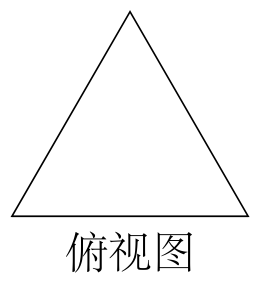
\includegraphics[width=2.5cm]{GaoKao/images/2011/liaoning_liberal/q8_fig1.png}
\end{center}

        {\centering\begin{tabular*}{\linewidth}{@{}@{\extracolsep{\fill}}llll@{}}
          \text{A. }\(4\)  &  \text{B. }\(2\sqrt{3}\)  &  \text{C. }\(2\)  &  \text{D. }\(\sqrt{3}\)
        \end{tabular*}\par}

        \item 执行下面的程序框图，如果输入的 \(n\) 是 4，则输出的 \(p\) 是（\quad）

\begin{center}
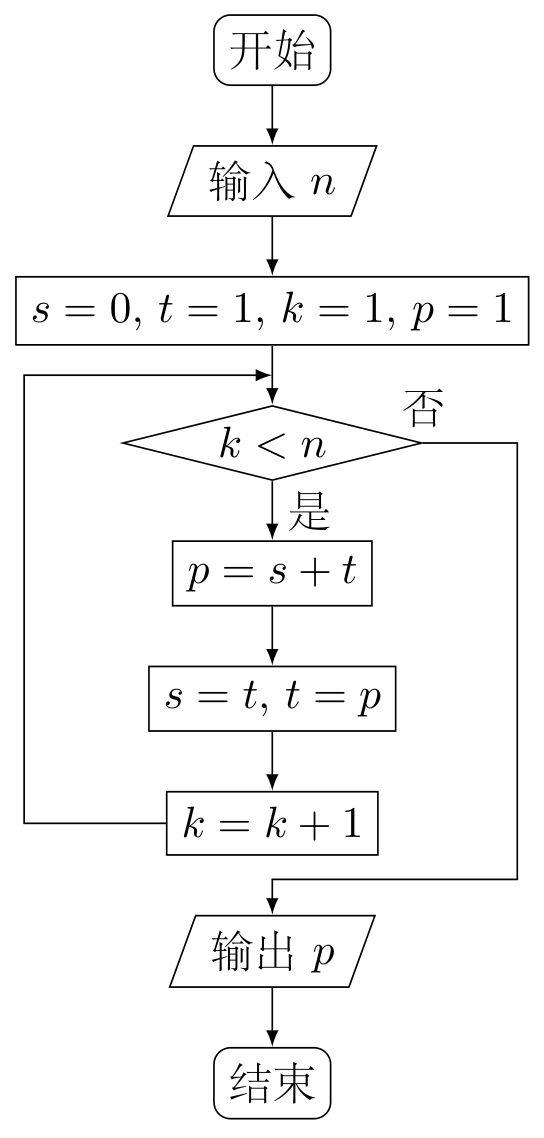
\includegraphics[width=0.52\linewidth]{GaoKao/images/2011/liaoning_liberal/q10_fig1.png}
\end{center}

        {\centering\begin{tabular*}{\linewidth}{@{}@{\extracolsep{\fill}}llll@{}}
          \text{A. }\(8\)  &  \text{B. }\(5\)  &  \text{C. }\(3\)  &  \text{D. }\(2\)
        \end{tabular*}\par}

        \item 已知球的直径 \(SC = 4\)，\(A\)，\(B\) 是该球球面上的两点，\(AB = 2\)，\(\angle ASC = \angle BSC = 45^\circ\)，则棱锥 \(S-ABC\) 的体积为（\quad）

        {\centering\begin{tabular*}{\linewidth}{@{}@{\extracolsep{\fill}}llll@{}}
          \text{A. }\(\frac{\sqrt{3}}{3}\)  &  \text{B. }\(\frac{2\sqrt{3}}{3}\)  &  \text{C. }\(\frac{4\sqrt{3}}{3}\)  &  \text{D. }\(\frac{5\sqrt{3}}{3}\)
        \end{tabular*}\par}

        \item \(f(x)\) 的定义域为 \(\mathbb{R}\)，\(f(-1) = 2\)，对任意 \(x \in \mathbb{R}\)，\(f'(x) > 2\)，则 \(f(x) > 2x + 4\) 的解集为（\quad）

        {\centering\begin{tabular*}{\linewidth}{@{}@{\extracolsep{\fill}}llll@{}}
          \text{A. }\((-1,1)\)  &  \text{B. }\((-1,+\infty)\)  &  \text{C. }\((-\infty,-1)\)  &  \text{D. }\((-\infty,+\infty)\)
        \end{tabular*}\par}

        \item 已知函数 \(f(x) = A \tan(\omega x + \varphi)\)（\(\omega > 0\)，\(|\varphi| < \frac{\pi}{2}\)），\(y = f(x)\) 的部分图象如图，则 \(f\left(\frac{\pi}{24}\right) =\)（\quad）

\begin{center}
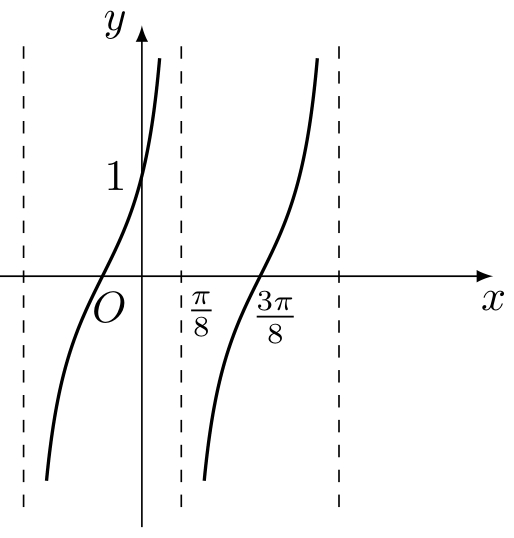
\includegraphics[width=7.4cm]{GaoKao/images/2011/liaoning_liberal/q12_fig1.png}
\end{center}

        {\centering\begin{tabular*}{\linewidth}{@{}@{\extracolsep{\fill}}llll@{}}
          \text{A. }\(2 + \sqrt{3}\)  &  \text{B. }\(\sqrt{3}\)  &  \text{C. }\(\frac{\sqrt{3}}{3}\)  &  \text{D. }\(2 - \sqrt{3}\)
        \end{tabular*}\par}

    \end{enumerate}

\end{description}

\begin{description}

    \item[二、填空题]

    \begin{enumerate}[leftmargin=5pt]

      \addtocounter{enumi}{+12}

        \item 已知圆 \(C\) 经过 \(A(5,1)\)，\(B(1,3)\) 两点，圆心在 \(x\) 轴上，则 \(C\) 的方程为\rule[-0.3ex]{3em}{0.4pt}.

        \item 调查了某地若干户家庭的年收入 \(x\)（单位：万元）和年饮食支出 \(y\)（单位：万元）. 调查显示年收入 \(x\) 与年饮食支出 \(y\) 具有线性相关关系，并由调查数据得到 \(y\) 对 \(x\) 的回归直线方程：\(\hat{y} = 0.254x + 0.321\). 由回归直线方程可知，家庭年收入每增加 \(1\) 万元，年饮食支出平均增加\rule[-0.3ex]{3em}{0.4pt} 万元.

        \item \(S_{n}\) 为等差数列 \(\{a_{n}\}\) 的前 \(n\) 项和，\(S_{2} = S_{6}\)，\(a_{4} = 1\)，则 \(a_{5} =\)\rule[-0.3ex]{3em}{0.4pt}.

        \item 已知函数 \(f(x) = {\mathrm{e}}^{x} - 2x + a\) 有零点，则 \(a\) 的取值范围是\rule[-0.3ex]{3em}{0.4pt}.

    \end{enumerate}

\end{description}

\begin{description}

    \item[三、解答题]

    \begin{enumerate}[leftmargin=5pt]

      \addtocounter{enumi}{+16}

        \item \(\triangle ABC\) 的三个内角 \(A\)，\(B\)，\(C\) 所对的边分别为 \(a\)，\(b\)，\(c\)，\(a \sin A \sin B + b \cos^{2} A = \sqrt{2}a\).
\begin{enumerate}
\item 求 \(\frac{b}{a}\)；
\item 若 \(c^{2} = b^{2} + \sqrt{3}a^{2}\)，求 \(B\).
\end{enumerate}

        \item 如图，四边形 \(ABCD\) 为正方形，\(QA \perp\) 平面 \(ABCD\)，\(PD \parallel QA\)，\(QA = AB = \frac{1}{2}PD\).
\begin{enumerate}
\item 证明：\(PQ \perp\) 平面 \(DCQ\)；
\item 求棱锥 \(Q-ABCD\) 的体积与棱锥 \(P-DCQ\) 的体积比值.
\end{enumerate}

\begin{center}
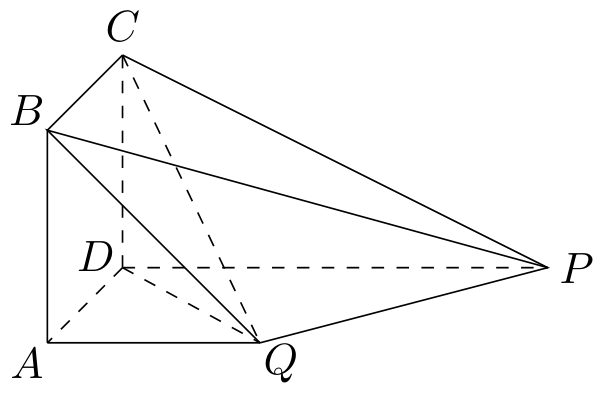
\includegraphics[width=7.2cm]{GaoKao/images/2011/liaoning_liberal/q18_fig1.png}
\end{center}

        \item 某农场计划种植某种新作物，为此对这种作物的两个品种（分别称为品种甲和品种乙）进行田间试验，选取两大块地. 每大块地分成 \(n\) 小块地. 在总共 \(2n\) 小块地中，随机选 \(n\) 小块地种植品种甲，另外 \(n\) 小块地种植品种乙.
\begin{enumerate}
\item 假设 \(n = 2\)，求第一大块地都种植品种甲的概率；
\item 试验时每大块地分成 \(8\) 小块，即 \(n = 8\)，试验结束后得到品种甲和品种乙在各小块地上的每公顷产量（单位：\(\mathrm{kg/hm^2}\)）如下表：
\begin{center}
\begin{tabular}{c|cccccccc}
\hline
品种甲 & \(403\) & \(397\) & \(390\) & \(404\) & \(388\) & \(400\) & \(412\) & \(406\) \\
\hline
品种乙 & \(419\) & \(403\) & \(412\) & \(418\) & \(408\) & \(423\) & \(400\) & \(413\) \\
\hline
\end{tabular}
\end{center}
分别求品种甲和品种乙每公顷产量的样本平均数和样本方差；根据试验结果，你应该种植哪一品种？
\end{enumerate}

附：样本数据 \(x_{1}\)，\(x_{2}\)，\(\cdots\)，\(x_{n}\) 的样本方差 \(s^{2} = \frac{1}{n}[(x_{1} - \overline{x})^{2} + (x_{2} - \overline{x})^{2} + \cdots + (x_{n} - \overline{x})^{2}]\)，其中 \(\overline{x}\) 为样本平均数.

        \item 设函数 \(f(x) = x + ax^{2} + b \ln x\)，曲线 \(y = f(x)\) 过 \(P(1,0)\)，且在 \(P\) 点处的切线斜率为 \(2\).
\begin{enumerate}
\item 求 \(a\)，\(b\) 的值；
\item 证明：\(f(x) \leqslant 2x - 2\).
\end{enumerate}

        \item 如图，已知椭圆 \(C_{1}\) 的中心在原点 \(O\)，长轴左，右端点 \(M\)，\(N\) 在 \(x\) 轴上，椭圆 \(C_{2}\) 的短轴为 \(MN\)，且 \(C_{1}\)，\(C_{2}\) 的离心率都为 \(e\). 直线 \(l \perp MN\)，\(l\) 与 \(C_{1}\) 交于两点，与 \(C_{2}\) 交于两点，这四点按纵坐标从大到小依次为 \(A\)，\(B\)，\(C\)，\(D\).
\begin{enumerate}
\item 设 \(e = \frac{1}{2}\)，求 \(|BC|\) 与 \(|AD|\) 的比值；
\item 当 \(e\) 变化时，是否存在直线 \(l\)，使得 \(BO \parallel AN\)，并说明理由.
\end{enumerate}

\begin{center}
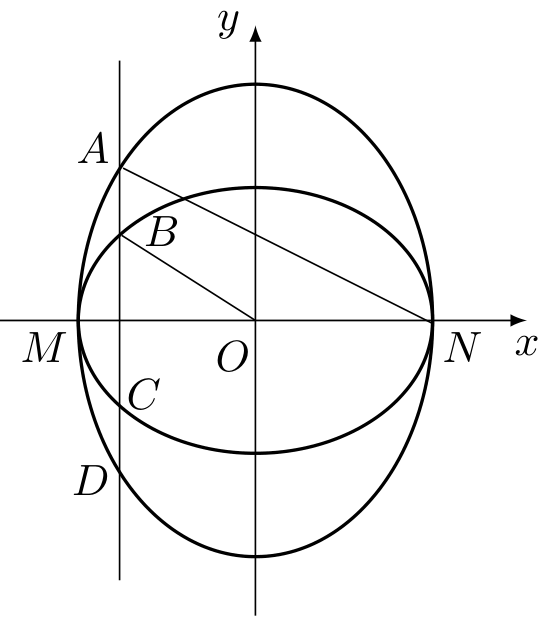
\includegraphics[width=2.0cm]{GaoKao/images/2011/liaoning_liberal/q21_fig1.png}
\end{center}

    \end{enumerate}

\end{description}

\begin{description}

    \item[四、选考题]

    \begin{enumerate}[leftmargin=5pt]

      \addtocounter{enumi}{+21}

        \item \textbf{【选修4-1：几何证明选讲】}

如图，\(A\)，\(B\)，\(C\)，\(D\) 四点在同一圆上，\(AD\) 的延长线与 \(BC\) 的延长线交于 \(E\) 点，且 \(EC = ED\).
\begin{enumerate}
\item 证明： \(CD \parallel AB\)；
\item 延长 \(CD\) 到 \(F\)，延长 \(DC\) 到 \(G\)，使得 \(EF = EG\)，证明： \(A\)，\(B\)，\(G\)，\(F\) 四点共圆.
\end{enumerate}

\begin{center}
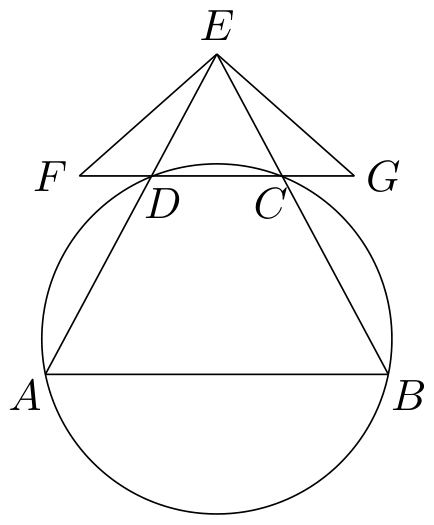
\includegraphics[width=5.4cm]{GaoKao/images/2011/liaoning_liberal/q22_fig1.png}
\end{center}

        \item \textbf{【选修4-4：坐标系与参数方程】}

在平面直角坐标系 \(xOy\) 中，曲线 \(C_{1}\) 的参数方程为 \(\begin{cases}
x = \cos \varphi,\\
y = \sin \varphi,
\end{cases}\)（\(\varphi\) 为参数）. 曲线 \(C_{2}\) 的参数方程为 \(\begin{cases}
x = a\cos \varphi,\\
y = b\sin \varphi,
\end{cases}\)（\(a > b > 0\)，\(\varphi\) 为参数）. 在以 \(O\) 为极点，\(x\) 轴的正半轴为极轴的极坐标系中，射线 \(l: \theta = \alpha\) 与 \(C_{1}\)，\(C_{2}\) 各有一个交点. 当 \(\alpha = 0\) 时，这两个交点间的距离为 \(2\)，当 \(\alpha = \frac{\pi}{2}\) 时，这两个交点重合.
\begin{enumerate}
\item 分别说明 \(C_{1}\)，\(C_{2}\) 是什么曲线，并求出 \(a\) 与 \(b\) 的值；
\item 设当 \(\alpha = \frac{\pi}{2}\) 时，\(l\) 与 \(C_{1}\)，\(C_{2}\) 的交点分别为 \(A_{1}\)，\(B_{1}\)，当 \(\alpha = -\frac{\pi}{4}\) 时，\(l\) 与 \(C_{1}\)，\(C_{2}\) 的交点分别为 \(A_{2}\)，\(B_{2}\)，求四边形 \(A_{1}A_{2}B_{2}B_{1}\) 的面积.
\end{enumerate}

        \item \textbf{【选修4-5：不等式选讲】}

已知函数 \(f(x) = |x - 2| - |x - 5|\).
\begin{enumerate}
\item 证明： \(-3 \leqslant f(x) \leqslant 3\)；
\item 求不等式 \(f(x) \geqslant x^{2} - 8x + 15\) 的解集.
\end{enumerate}

    \end{enumerate}

\end{description}


\subsection{2011年上海卷（理）}\label{gk:2011年上海卷（理）}

\begin{description}

    \item[一、填空题]

    \begin{enumerate}[leftmargin=5pt]

        \item 函数 \( f(x) = \frac{1}{x - 2} \) 的反函数为 \( f^{-1}(x) = \)\rule[-0.3ex]{3em}{0.4pt}.

        \item 若全集 \(U = \mathbb{R}\)，集合 \(A = \{x \mid x \geqslant 1\} \cup \{x \mid x \leqslant 0\}\)，则 \(\complement_U A =\rule[-0.3ex]{3em}{0.4pt}\).

        \item 设 \(m\) 为常数，若点 \(F(0,5)\) 是双曲线 \(\frac{y^2}{m} - \frac{x^2}{9} = 1\) 的一个焦点，则 \(m =\rule[-0.3ex]{3em}{0.4pt}\).

        \item 不等式 \(\frac{x + 1}{x} \leqslant 3\) 的解集为\rule[-0.3ex]{3em}{0.4pt}.

        \item 在极坐标系中，直线 \(\rho(2\cos \theta + \sin \theta) = 2\) 与直线 \(\rho\cos \theta = 1\) 的夹角大小为\rule[-0.3ex]{3em}{0.4pt}. （结果用反三角函数值表示）

        \item 在相距 2 千米的 \(A, B\) 两点处测量目标 \(C\)，若 \(\angle CAB = 75^{\circ}\)，\(\angle CBA = 60^{\circ}\)，则 \(A, C\) 两点之间的距离为\rule[-0.3ex]{3em}{0.4pt}\text{千米}.

        \item 若圆锥的侧面积为 \(2\pi\)，底面积为 \(\pi\)，则该圆锥的体积为\rule[-0.3ex]{3em}{0.4pt}.

        \item 函数 \( y = \sin \left(\frac{\pi}{2} + x\right) \cos \left(\frac{\pi}{6} - x\right) \) 的最大值为\rule[-0.3ex]{3em}{0.4pt}.

        \item 马老师从课本上抄录一个随机变量 \(\xi\) 的概率分布列如下表：

\begin{center}
\begin{tabular}{|c|c|c|c|}
\hline
\(X\) & 1 & 2 & 3 \\
\hline
\(P(\xi=x)\) & ? & ! & ? \\
\hline
\end{tabular}
\end{center}

请小牛同学计算 \( \xi \) 的数学期望，尽管“!”处无法完全看清，且两个“?”处字迹模糊，但能肯定这两个“?”处的数值相同. 据此，小牛给出了正确答案 \(E(\xi)=\)\rule[-0.3ex]{3em}{0.4pt}.

        \item 行列式 \(\begin{vmatrix}a & b\\ c & d \end{vmatrix}\) （\(a,b,c,d\in \{-1,1,2\}\)）所有可能的值中，最大的是\rule[-0.3ex]{3em}{0.4pt}.

        \item 在正三角形 \(ABC\) 中，\(D\) 是 \(BC\) 上的点. 若 \(AB = 3\)，\(BD = 1\)，则 \(\overrightarrow{AB} \cdot \overrightarrow{AD} =\rule[-0.3ex]{3em}{0.4pt}.\)

        \item 随机抽取的 9 位同学中，至少有 2 位同学在同一月份出生的概率为\rule[-0.3ex]{3em}{0.4pt}. （默认每个月的天数相同，结果精确到 0.001）

        \item 设 \(g(x)\) 是定义在 \(\mathbb{R}\) 上，以 1 为周期的函数，若函数 \(f(x) = x + g(x)\) 在区间 \([3,4]\) 上的值域为 \([-2,5]\)，则 \(f(x)\) 在区间 \([-10,10]\) 上的值域为\rule[-0.3ex]{3em}{0.4pt}.

        \item 已知点 \(O(0,0)\)，\(Q_0(0,1)\) 和点 \(R_0(3,1)\)，记 \(Q_0R_0\) 的中点为 \(P_1\)，取 \(Q_0P_1\) 和 \(P_1R_0\) 中的一条，记其端点为 \(Q_1\)，\(R_1\)，使之满足 \((|OQ_1| - 2)(|OR_1| - 2) < 0\)，记 \(Q_1R_1\) 的中点为 \(P_2\)，取 \(Q_1P_2\) 和 \(P_2R_1\) 中的一条，记其端点为 \(Q_2\)，\(R_2\)，使之满足 \((|OQ_2| - 2)(|OR_2| - 2) < 0\). 依次下去，得到 \(P_1\)，\(P_2\)，\(\cdots\)，\(P_n\)，\(\cdots\)，则 \(\lim\limits_{n \to \infty} \left|Q_0P_n\right| =\rule[-0.3ex]{3em}{0.4pt} \).

    \end{enumerate}

\end{description}

\begin{description}

    \item[二、选择题]

    \begin{enumerate}[leftmargin=5pt]

      \addtocounter{enumi}{+14}

        \item 若 \(a\)，\(b \in \mathbb{R}\)，且 \(ab > 0\)，则下列不等式中，恒成立的是（\quad）

        {\centering\begin{tabular*}{\linewidth}{@{}@{\extracolsep{\fill}}llll@{}}
          \text{A. }\(a^{2} + b^{2} > 2ab\)  &  \text{B. }\(a + b \geqslant 2\sqrt{ab}\)  &  \text{C. }\(\frac{1}{a} + \frac{1}{b} > \frac{2}{\sqrt{ab}}\)  &  \text{D. }\(\frac{b}{a} + \frac{a}{b} \geqslant 2\)
        \end{tabular*}\par}

        \item 下列函数中，既是偶函数，又是在区间 \((0,+\infty)\) 上单调递减的函数是（\quad）

        {\centering\begin{tabular*}{\linewidth}{@{}@{\extracolsep{\fill}}llll@{}}
          \text{A. }\(y = \ln \frac{1}{|x|}\)  &  \text{B. }\(y = x^{3}\)  &  \text{C. }\(y = 2^{|x|}\)  &  \text{D. }\(y = \cos x\)
        \end{tabular*}\par}

        \item 设 \(A_1\)，\(A_2\)，\(A_3\)，\(A_4\)，\(A_5\) 是平面上给定的 5 个不同点，则使 \(\overrightarrow{MA_1} + \overrightarrow{MA_2} + \overrightarrow{MA_3} + \overrightarrow{MA_4} + \overrightarrow{MA_5} = \vec{0}\) 成立的点 \(M\) 的个数为（\quad）

        {\centering\begin{tabular*}{\linewidth}{@{}@{\extracolsep{\fill}}llll@{}}
          \text{A. }\(0\)  &  \text{B. }\(1\)  &  \text{C. }\(5\)  &  \text{D. }\(10\)
        \end{tabular*}\par}

        \item 设 \(\{a_n\}\) 是各项为正数的无穷数列，\(A_i\) 是边长为 \(a_i\)，\(a_{i+1}\) 的矩形面积 （\(i = 1, 2, \cdots\)），则 \(\{A_n\}\) 为等比数列的充要条件为（\quad）

        {\centering\begin{tabular*}{\linewidth}{@{}@{\extracolsep{\fill}}llll@{}}
          \text{A. }\(\{a_n\}\) 是等比数列  &  \text{B. }\(\{a_1, a_3, \cdots, a_{2n-1}, \cdots\}\) 或 \(\{a_2, a_4, \cdots, a_{2n}, \cdots\}\) 是等比数列  &  \text{C. }\(\{a_1, a_3, \cdots, a_{2n-1}, \cdots\}\) 和 \(\{a_2, a_4, \cdots, a_{2n}, \cdots\}\) 均是等比数列  &  \text{D. }\(\{a_1, a_3, \cdots, a_{2n-1}, \cdots\}\) 和 \(\{a_2, a_4, \cdots, a_{2n}, \cdots\}\) 均是等比数列，且公比相同
        \end{tabular*}\par}

    \end{enumerate}

\end{description}

\begin{description}

    \item[三、解答题]

    \begin{enumerate}[leftmargin=5pt]

      \addtocounter{enumi}{+18}

        \item 已知复数 \(z_1\) 满足 \((z_1 - 2)(1 + \i) = 1 - \i\)（\(\i\) 为虚数单位），复数 \(z_2\) 的虚部为 2，且 \(z_1 \cdot z_2\) 是实数，求 \(z_2\).

        \item 已知函数 \(f(x) = a \cdot 2^{x} + b \cdot 3^{x}\)，其中常数 \(a\)，\(b\) 满足 \(a \cdot b \neq 0\).

\begin{enumerate}
\item 若 \(a \cdot b > 0\)，判断函数 \(f(x)\) 的单调性；
\item 若 \(a \cdot b < 0\)，求 \(f(x+1) > f(x)\) 时的 \(x\) 的取值范围.
\end{enumerate}

        \item 已知 \(ABCD - A_{1}B_{1}C_{1}D_{1}\) 是底面边长为 1 的正四棱柱，\(O_1\) 为 \(A_1C_1\) 与 \(B_1D_1\) 的交点.

\begin{enumerate}
\item 设 \(AB_1\) 与底面 \(A_1B_1C_1D_1\) 所成角的大小为 \(\alpha\)，二面角 \(A - B_{1}D_{1} - A_1\) 的大小为 \(\beta\). 求证：\(\tan \beta = \sqrt{2}\tan \alpha\)；
\item 若点 \(C\) 到平面 \(AB_1D_1\) 的距离为 \(\frac{4}{3}\)，求正四棱柱 \(ABCD - A_{1}B_{1}C_{1}D_{1}\) 的高.
\end{enumerate}

\begin{center}
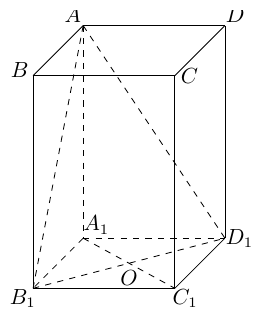
\includegraphics[width=5.3cm]{GaoKao/images/2011/shanghai_science/q21_fig1.png}
\end{center}

        \item 已知数列 \(\{a_n\}\) 和 \(\{b_n\}\) 的通项公式分别为 \(a_n = 3n + 6\)，\(b_n = 2n + 7\) （\(n \in \mathbf{N}^{*}\)），将集合 \(\{x \mid x = a_n, n \in \mathbf{N}^{*}\} \cup \{x \mid x = b_n, n \in \mathbf{N}^{*}\}\) 中的元素从小到大依次排列，构成数列 \(c_1\)，\(c_2\)，\(c_3\)，\(\cdots\)，\(c_n\)，\(\cdots\).

\begin{enumerate}
\item 求 \(c_1\)，\(c_2\)，\(c_3\)，\(c_4\)；
\item 求证：在数列 \(\{a_n\}\) 中，但不在数列 \(\{b_n\}\) 中的项恰为 \(a_2\)，\(a_4\)，\(\cdots\)，\(a_{2n}\)，\(\cdots\)；
\item 求数列 \(\{c_n\}\) 的通项公式.
\end{enumerate}

        \item 已知平面上的线段 \(l\) 及点 \(P\)，在 \(l\) 上任取一点 \(Q\)，线段 \(PQ\) 长度的最小值称为点 \(P\) 到线段 \(l\) 的距离，记作 \(d(P, l)\).

\begin{enumerate}
\item 求点 \(P(1,1)\) 到线段 \(l: x - y - 3 = 0\)（\(3 \leqslant x \leqslant 5\)）的距离 \(d(P, l)\)；
\item 设 \(l\) 是长为 2 的线段，求点的集合 \(D = \{P \mid d(P, l) \leqslant 1\}\) 所表示的图形面积；
\item 写出到两条线段 \(l_1\)，\(l_2\) 距离相等的点的集合 \(\Omega = \{P \mid d(P, l_1) = d(P, l_2)\}\)，其中 \(l_1 = AB\)，\(l_2 = CD\)，\(A\)，\(B\)，\(C\)，\(D\) 是下列三组点中的一组.

\begin{enumerate}
\item \(A(1,3)\)，\(B(1,0)\)，\(C(-1,3)\)，\(D(-1,0)\).
\item \(A(1,3)\)，\(B(1,0)\)，\(C(-1,3)\)，\(D(-1,-2)\).
\item \(A(0,1)\)，\(B(0,0)\)，\(C(0,0)\)，\(D(2,0)\).
\end{enumerate}
\end{enumerate}

    \end{enumerate}

\end{description}


\subsection{2011年上海卷（文）}\label{gk:2011年上海卷（文）}

\begin{description}

    \item[一、填空题]

    \begin{enumerate}[leftmargin=5pt]

        \item 若全集 \(U = \mathbb{R}\)，集合 \(A = \{x \mid x \geqslant 1\}\)，则 \(\complement_U A =\rule[-0.3ex]{3em}{0.4pt}\).

        \item \(\lim\limits_{n\to \infty}\left(1 - \frac{3n}{n + 3}\right) =\rule[-0.3ex]{3em}{0.4pt}\).

        \item 若函数 \( f(x) = 2x + 1 \) 的反函数为 \( f^{-1}(x) \)，则 \( f^{-1}(-2) = \)\rule[-0.3ex]{3em}{0.4pt}.

        \item 函数 \( y = 2\sin x - \cos x \) 的最大值为\rule[-0.3ex]{3em}{0.4pt}.

        \item 若直线 \(l\) 过点 \( (3,4) \)，且 \( (1,2) \) 是它的一个法向量，则直线 \(l\) 的方程为\rule[-0.3ex]{3em}{0.4pt}.

        \item 不等式 \(\frac{1}{x} < 1\) 的解集为\rule[-0.3ex]{3em}{0.4pt}.

        \item 若一个圆锥的主视图（如图所示）是边长为 \(3\)，\(3\)，\(2\) 的三角形，则该圆锥的侧面积为\rule[-0.3ex]{3em}{0.4pt}.
\begin{center}
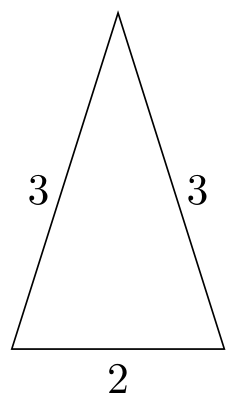
\includegraphics[width=2.3cm]{GaoKao/images/2011/shanghai_liberal/q7_fig1.png}
\end{center}

        \item 在相距 \(2\mathrm{~km}\) 的 \(A\)，\(B\) 两点处测量目标点 \(C\)，若 \(\angle CAB = 75^{\circ}\)，\(\angle CBA = 60^{\circ}\)，则 \(A\)，\(C\) 两点之间的距离是\rule[-0.3ex]{3em}{0.4pt}\(\mathrm{~km}\).

        \item 若变量 \(x\)，\(y\) 满足条件 \(\begin{cases}
3x - y \leqslant 0,\\
x - 3y + 5 \geqslant 0,
\end{cases}\) 则 \(z = x + y\) 的最大值为\rule[-0.3ex]{3em}{0.4pt}.

        \item 课题组进行城市空气质量调查，按地域把 \(24\) 个城市分成甲，乙，丙三组，对应的城市数分别为 \(4\)，\(12\)，\(8\)，若用分层抽样抽取 \(6\) 个城市，则丙组中应抽取的城市数为\rule[-0.3ex]{3em}{0.4pt}.

        \item 行列式 \(\begin{vmatrix}a & b\\ c & d \end{vmatrix}\) （\(a, b, c, d \in \{-1,1,2\}\)） 所有可能的值中，最大的是\rule[-0.3ex]{3em}{0.4pt}.

        \item 在正三角形 \(ABC\) 中，\(D\) 是 \(BC\) 上的点. 若 \(AB = 3\)，\(BD = 1\)，则 \(\overrightarrow{AB} \cdot \overrightarrow{AD} =\)\rule[-0.3ex]{3em}{0.4pt}.

        \item 随机抽取的 \(9\) 位同学中，至少有 \(2\) 位同学在同一月份出生的概率为\rule[-0.3ex]{3em}{0.4pt}（默认每个月的天数相同，结果精确到 \(0.001\)）.

        \item 设 \(g(x)\) 是定义在 \(\mathbb{R}\) 上，以 1 为周期的函数，若函数 \(f(x) = x + g(x)\) 在区间 \([0,1]\) 上的值域为 \([-2,5]\)，则 \(f(x)\) 在区间 \([0,3]\) 上的值域为\rule[-0.3ex]{3em}{0.4pt}.

    \end{enumerate}

\end{description}

\begin{description}

    \item[二、选择题]

    \begin{enumerate}[leftmargin=5pt]

      \addtocounter{enumi}{+14}

        \item 下列函数中，既是偶函数，又在区间 \((0, +\infty)\) 上单调递减的是（\quad）

        {\centering\begin{tabular*}{\linewidth}{@{}@{\extracolsep{\fill}}llll@{}}
          \text{A. }\( y = x^{-2} \)  &  \text{B. }\( y = x^{-1} \)  &  \text{C. }\( y = x^{2} \)  &  \text{D. }\( y = x^{\frac{1}{3}} \)
        \end{tabular*}\par}

        \item 若 \(a\)，\(b \in \mathbb{R}\)，且 \(ab > 0\)，则下列不等式中，恒成立的是（\quad）

        {\centering\begin{tabular*}{\linewidth}{@{}@{\extracolsep{\fill}}llll@{}}
          \text{A. }\(a^2 + b^2 > 2ab\)  &  \text{B. }\(a + b \geqslant 2\sqrt{ab}\)  &  \text{C. }\(\frac{1}{a} + \frac{1}{b} > \frac{2}{\sqrt{ab}}\)  &  \text{D. }\(\frac{b}{a} + \frac{a}{b} \geqslant 2\)
        \end{tabular*}\par}

        \item 若三角方程 \(\sin x = 0\) 与 \(\sin 2x = 0\) 的解集分别为 \(E\)，\(F\)，则（\quad）

        {\centering\begin{tabular*}{\linewidth}{@{}@{\extracolsep{\fill}}llll@{}}
          \text{A. }\(E \subsetneq F\)  &  \text{B. }\(E \supsetneq F\)  &  \text{C. }\(E = F\)  &  \text{D. }\(E \cap F = \varnothing\)
        \end{tabular*}\par}

        \item 设 \(A_{1}\)，\(A_{2}\)，\(A_{3}\)，\(A_{4}\) 是平面上给定的 4 个不同点，则使 \(\overrightarrow{MA_{1}} + \overrightarrow{MA_{2}} + \overrightarrow{MA_{3}} + \overrightarrow{MA_{4}} = \overrightarrow{0}\) 成立的点 \(M\) 的个数为（\quad）

        {\centering\begin{tabular*}{\linewidth}{@{}@{\extracolsep{\fill}}llll@{}}
          \text{A. }0  &  \text{B. }1  &  \text{C. }2  &  \text{D. }4
        \end{tabular*}\par}

    \end{enumerate}

\end{description}

\begin{description}

    \item[三、解答题]

    \begin{enumerate}[leftmargin=5pt]

      \addtocounter{enumi}{+18}

        \item 已知复数 \(z_{1}\) 满足 \((z_{1} - 2)(1 + \i) = 1 - \i\)（\(\i\) 为虚数单位），复数 \(z_{2}\) 的虚部为 2，且 \(z_{1} \cdot z_{2}\) 是实数，求 \(z_{2}\).

        \item 已知 \(ABCD - A_{1}B_{1}C_{1}D_{1}\) 是底面边长为 \(1\) 的正四棱柱，高 \(AA_{1} = 2\)，求：
\begin{enumerate}
\item 异面直线 \(BD\) 与 \(AB_{1}\) 所成角的余弦值；
\item 四面体 \(AB_{1}D_{1}C\) 的体积.
\end{enumerate}
\begin{center}
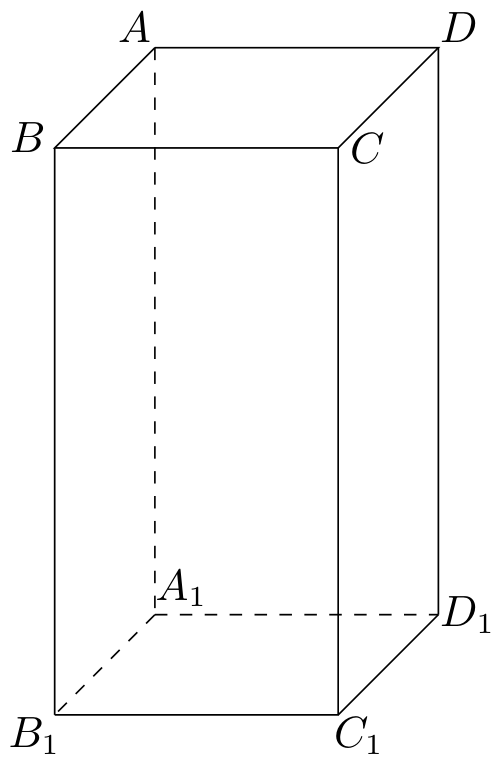
\includegraphics[width=5.0cm]{GaoKao/images/2011/shanghai_liberal/q20_fig1.png}
\end{center}

        \item 已知函数 \(f(x) = a \cdot 2^{x} + b \cdot 3^{x}\)，其中常数 \(a\)，\(b\) 满足 \(a \cdot b \neq 0\).
\begin{enumerate}
\item 若 \(a \cdot b > 0\)，判断函数 \(f(x)\) 的单调性；
\item 若 \(a \cdot b < 0\)，求 \(f(x + 1) > f(x)\) 时的 \(x\) 的取值范围.
\end{enumerate}

        \item 已知椭圆 \(C: \frac{x^2}{m^2} + y^{2} = 1\)（常数 \(m > 1\)），\(P\) 是曲线 \(C\) 上的动点，\(M\) 是曲线 \(C\) 的右顶点，定点 \(A\) 的坐标为 \((2,0)\).
\begin{enumerate}
\item 若 \(M\) 与 \(A\) 重合，求曲线 \(C\) 的焦点坐标；
\item 若 \(m = 3\)，求 \(|PA|\) 的最大值与最小值；
\item 若 \(|PA|\) 的最小值为 \(|MA|\)，求实数 \(m\) 的取值范围.
\end{enumerate}

        \item 已知数列 \(\{a_{n}\}\) 和 \(\{b_{n}\}\) 的通项公式分别为 \(a_{n} = 3n + 6\)，\(b_{n} = 2n + 7\)（\(n \in \mathbf{N}^{*}\)），将集合 \(\{x \mid x = a_{n}, n \in \mathbf{N}^{*}\} \cup \{x \mid x = b_{n}, n \in \mathbf{N}^{*}\}\) 中的元素从小到大依次排列，构成数列 \(c_{1}\)，\(c_{2}\)，\(c_{3}\)，\(\cdots\)，\(c_{n}\)，\(\cdots\).
\begin{enumerate}
\item 求三个最小的数，使它们既是数列 \(\{a_{n}\}\) 中的项，又是数列 \(\{b_{n}\}\) 中的项；
\item 数列 \(c_{1}\)，\(c_{2}\)，\(c_{3}\)，\(\cdots\)，\(c_{40}\) 中有多少项不是数列 \(\{b_{n}\}\) 中的项？请说明理由；
\item 求数列 \(\{c_{n}\}\) 的前 \(4n\) 项和 \(S_{4n}\)（\(n \in \mathbf{N}^{*}\)）.
\end{enumerate}

    \end{enumerate}

\end{description}


\subsection{2011年四川卷（理）}\label{gk:2011年四川卷（理）}

\begin{description}

    \item[一、选择题]

    \begin{enumerate}[leftmargin=5pt]

        \item 有一个容量为 66 的样本，数据的分组及各组的频数如下：
\begin{center}
\begin{tabular}{cccc}
\([11.5,15.5)\) & \([15.5,19.5)\) & \([19.5,23.5)\) & \([23.5,27.5)\)\\
2 & 4 & 9 & 18\\
\([27.5,31.5)\) & \([31.5,35.5)\) & \([35.5,39.5)\) & \([39.5,43.5)\)\\
11 & 12 & 7 & 3
\end{tabular}
\end{center}
根据样本的频率分布，估计数据落在 \([31.5,43.5)\) 的概率约是（\quad）

        {\centering\begin{tabular*}{\linewidth}{@{}@{\extracolsep{\fill}}llll@{}}
          \text{A. }\(\frac{1}{6}\)  &  \text{B. }\(\frac{1}{3}\)  &  \text{C. }\(\frac{1}{2}\)  &  \text{D. }\(\frac{2}{3}\)
        \end{tabular*}\par}

        \item 复数 \(-\i + \frac{1}{\i} =\)（\quad）

        {\centering\begin{tabular*}{\linewidth}{@{}@{\extracolsep{\fill}}llll@{}}
          \text{A. }\(-2\i\)  &  \text{B. }\(\frac{1}{2}\i\)  &  \text{C. }0  &  \text{D. }\(2\i\)
        \end{tabular*}\par}

        \item \(l_{1}\)，\(l_{2}\)，\(l_{3}\) 是空间三条不同的直线，则下列命题正确的是（\quad）

        {\centering\begin{tabular*}{\linewidth}{@{}@{\extracolsep{\fill}}llll@{}}
          \text{A. }\(l_{1} \perp l_{2}, l_{2} \perp l_{3} \Rightarrow l_{1} \parallel l_{3}\)  &  \text{B. }\(l_{1} \perp l_{2}\)，\(l_{2} \parallel l_{3} \Rightarrow l_{1} \perp l_{3}\)  &  \text{C. }\(l_{1} \parallel l_{2} \parallel l_{3} \Rightarrow l_{1}\)，\(l_{2}\)，\(l_{3}\) 共面  &  \text{D. }\(l_{1}\)，\(l_{2}\)，\(l_{3}\) 共点 \(\Rightarrow l_{1}\)，\(l_{2}\)，\(l_{3}\) 共面
        \end{tabular*}\par}

        \item 如图，正六边形 \(ABCDEF\) 中，\(\overrightarrow{BA} + \overrightarrow{CD} + \overrightarrow{EF} =\)（\quad）

\begin{center}
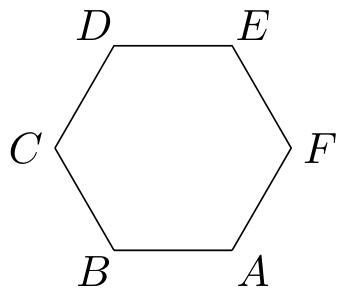
\includegraphics[width=4.3cm]{GaoKao/images/2011/sichuan_science/q4_fig1.png}
\end{center}

        {\centering\begin{tabular*}{\linewidth}{@{}@{\extracolsep{\fill}}llll@{}}
          \text{A. }0  &  \text{B. }\(\overrightarrow{BE}\)  &  \text{C. }\(\overrightarrow{AD}\)  &  \text{D. }\(\overrightarrow{CF}\)
        \end{tabular*}\par}

        \item “函数 \(f(x)\) 在点 \(x = x_0\) 处有定义”是“\(f(x)\) 在点 \(x = x_0\) 处连续”的（\quad）

        {\centering\begin{tabular*}{\linewidth}{@{}@{\extracolsep{\fill}}llll@{}}
          \text{A. }充分而不必要的条件  &  \text{B. }必要而不充分的条件  &  \text{C. }充要条件  &  \text{D. }既不充分也不必要的条件
        \end{tabular*}\par}

        \item 在 \(\triangle ABC\) 中，\(\sin^2 A \leqslant \sin^2 B + \sin^2 C - \sin B \sin C\)，则 \(A\) 的取值范围是（\quad）

        {\centering\begin{tabular*}{\linewidth}{@{}@{\extracolsep{\fill}}llll@{}}
          \text{A. }\(\left(0, \frac{\pi}{6}\right]\)  &  \text{B. }\(\left[\frac{\pi}{6},\pi\right)\)  &  \text{C. }\(\left(0, \frac{\pi}{3}\right]\)  &  \text{D. }\(\left[\frac{\pi}{3}, \pi\right)\)
        \end{tabular*}\par}

        \item 已知 \( f(x) \) 是 \( \mathbb{R} \) 上的奇函数，且当 \( x > 0 \) 时，\( f(x) = \left(\frac{1}{2}\right)^x + 1 \)，则 \( f(x) \) 的反函数的图象大致是（\quad）

        {\centering\begin{tabular*}{\linewidth}{@{}@{\extracolsep{\fill}}cccc@{}}
          \text{A. }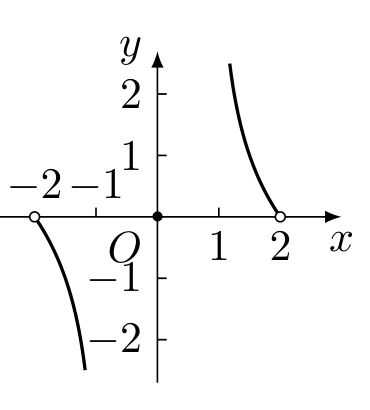
\includegraphics[width=0.15\paperwidth]{GaoKao/images/2011/sichuan_science/q7_choice_a.png}  &  \text{B. }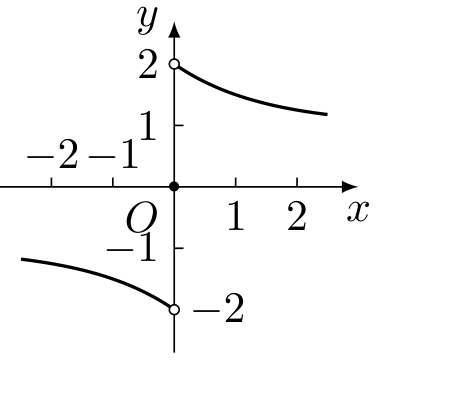
\includegraphics[width=0.15\paperwidth]{GaoKao/images/2011/sichuan_science/q7_choice_b.png}  &  \text{C. }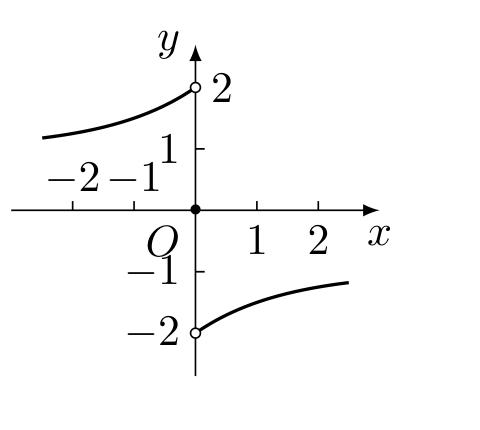
\includegraphics[width=0.15\paperwidth]{GaoKao/images/2011/sichuan_science/q7_choice_c.png}  &  \text{D. }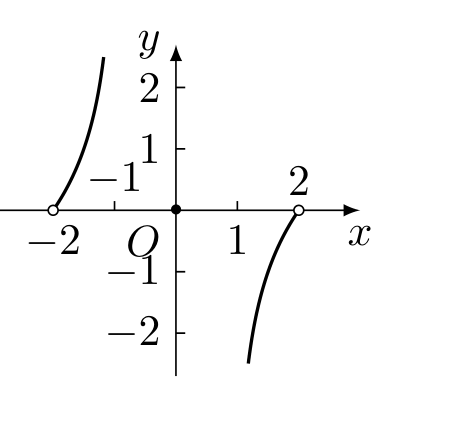
\includegraphics[width=0.15\paperwidth]{GaoKao/images/2011/sichuan_science/q7_choice_d.png}
        \end{tabular*}\par}

        \item 数列 \( \{a_{n}\} \) 的首项为 3，\( \{b_{n}\} \) 为等差数列且 \( b_{n}=a_{n+1}-a_{n} \)（\( n\in \mathbb{N}^{*} \)）. 若 \( b_{3}=-2 \)，\( b_{10}=12 \)，则 \( a_{8} =\)（\quad）

        {\centering\begin{tabular*}{\linewidth}{@{}@{\extracolsep{\fill}}llll@{}}
          \text{A. }0  &  \text{B. }3  &  \text{C. }8  &  \text{D. }11
        \end{tabular*}\par}

        \item 某运输公司有 12 名驾驶员和 19 名工人，有 8 辆载重量为 10 吨的甲型卡车和 7 辆载重量为 6 吨的乙型卡车. 某天需运往 \(A\) 地至少 72 吨的货物，派用的每辆车需载满且只能送一次，派用的每辆甲型卡车需配 2 名工人，运送一次可得利润 450 元；派用的每辆乙型卡车需配 1 名工人，运送一次可得利润 350 元. 该公司合理计划当天派用甲，乙卡车的车辆数，可得最大利润 \(z =\)（\quad）

        {\centering\begin{tabular*}{\linewidth}{@{}@{\extracolsep{\fill}}llll@{}}
          \text{A. }4650 元  &  \text{B. }4700 元  &  \text{C. }4900 元  &  \text{D. }5000 元
        \end{tabular*}\par}

        \item 在抛物线 \( y = x^{2} + ax - 5\) （\(a \neq 0\)）上取横坐标为 \(x_{1} = -4\)，\(x_{2} = 2\) 的两点，经过两点引一条割线，有平行于该割线的一条直线同时与抛物线和圆 \( 5x^{2} + 5y^{2} = 36 \) 相切，则抛物线顶点的坐标为（\quad）

        {\centering\begin{tabular*}{\linewidth}{@{}@{\extracolsep{\fill}}llll@{}}
          \text{A. }\((-2, -9)\)  &  \text{B. }\((0, -5)\)  &  \text{C. }\((2, -9)\)  &  \text{D. }\((1, -6)\)
        \end{tabular*}\par}

        \item 已知定义在 \( [0, +\infty) \) 上的函数 \( f(x) \) 满足 \( f(x) = 3f(x + 2) \)，当 \( x \in [0, 2) \) 时，\( f(x) = -x^{2} + 2x \). 设 \( f(x) \) 在 \( [2n - 2, 2n) \) 上的最大值为 \( a_{n} \) （\( n \in \mathbf{N}^{*} \)），且 \(\{a_{n}\}\) 的前 \(n\) 项和为 \(S_{n}\)，则 \(\lim\limits_{n\to\infty} S_{n} =\)（\quad）

        {\centering\begin{tabular*}{\linewidth}{@{}@{\extracolsep{\fill}}llll@{}}
          \text{A. }3  &  \text{B. }\(\frac{5}{2}\)  &  \text{C. }2  &  \text{D. }\(\frac{3}{2}\)
        \end{tabular*}\par}

        \item 在集合 \(\{1, 2, 3, 4, 5\}\) 中任取一个偶数 \(a\) 和一个奇数 \(b\) 构成以原点为起点的向量 \(\alpha = (a,b)\). 从所有得到的以原点为起点的向量中任取两个向量作为邻边作平行四边形. 记所有作成的平行四边形的个数为 \(n\)，其中面积不超过 4 的平行四边形的个数为 \(m\)，则 \(\frac{m}{n}=\)（\quad）

        {\centering\begin{tabular*}{\linewidth}{@{}@{\extracolsep{\fill}}llll@{}}
          \text{A. }\(\frac{4}{15}\)  &  \text{B. }\(\frac{1}{3}\)  &  \text{C. }\(\frac{2}{5}\)  &  \text{D. }\(\frac{2}{3}\)
        \end{tabular*}\par}

    \end{enumerate}

\end{description}

\begin{description}

    \item[二、填空题]

    \begin{enumerate}[leftmargin=5pt]

      \addtocounter{enumi}{+12}

        \item 计算 \(\left(\lg \frac{1}{4} - \lg 25\right) \div 100^{-\frac{1}{2}} =\rule[-0.3ex]{3em}{0.4pt}\).

        \item 双曲线 \(\frac{x^2}{64} - \frac{y^2}{36} = 1\) 上一点 \(P\) 到双曲线右焦点的距离是 4，那么点 \(P\) 到左准线的距离是\rule[-0.3ex]{3em}{0.4pt}.

        \item 如图，半径为 \(R\) 的球 \(O\) 中有一内接圆柱. 当圆柱的侧面积最大时，球的表面积与该圆柱的侧面积之差是\rule[-0.3ex]{3em}{0.4pt}.

\begin{center}
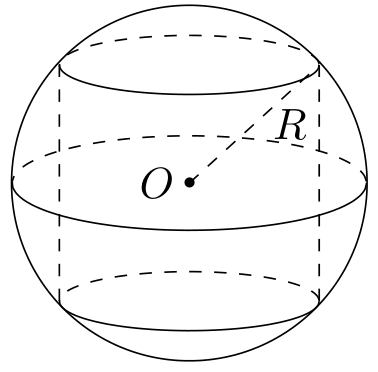
\includegraphics[width=4.4cm]{GaoKao/images/2011/sichuan_science/q15_fig1.png}
\end{center}

        \item 函数 \( f(x) \) 的定义域为 \(A\). 若 \(x_{1}\)，\(x_{2} \in A\) 且 \( f(x_{1}) = f(x_{2}) \) 时总有 \( x_{1} = x_{2} \)，则称 \( f(x) \) 为单函数. 例如，函数 \( f(x) = 2x + 1\) （\(x \in \mathbb{R}\)） 是单函数. 下列命题：
\begin{enumerate}
\item 函数 \( f(x)=x^{2} \)（\(x\in\mathbb{R}\)）是单函数；
\item 若 \(f(x)\) 为单函数，\(x_{1}\)，\(x_{2} \in A\) 且 \(x_{1} \neq x_{2}\)，则 \(f(x_{1}) \neq f(x_{2})\)；
\item 若 \(f: A \to B\) 为单函数，则对于任意 \(b \in B\)，它至多有一个原象；
\item 函数 \(f(x)\) 在某区间上具有单调性，
\end{enumerate}
则 \(f(x)\) 一定是单函数. 其中的真命题是\rule[-0.3ex]{3em}{0.4pt}.（写出所有真命题的编号）

    \end{enumerate}

\end{description}

\begin{description}

    \item[三、解答题]

    \begin{enumerate}[leftmargin=5pt]

      \addtocounter{enumi}{+16}

        \item 已知函数 \(f(x) = \sin \left( x + \frac{7\pi}{4} \right) + \cos \left( x - \frac{3\pi}{4} \right)\)，\(x \in \mathbb{R}\).
\begin{enumerate}
\item 求 \( f(x) \) 的最小正周期和最小值；
\item 已知 \(\cos(\beta-\alpha)=\frac{4}{5}\)，\(\cos(\beta+\alpha)=-\frac{4}{5}\)，\(0 < \alpha < \beta \leqslant \frac{\pi}{2}\)，求证： \(\left[f(\beta)\right]^2 - 2 = 0.\)
\end{enumerate}

        \item 本着健康，低碳的生活理念，租自行车骑游的人越来越多. 某自行车租车点的收费标准是每车每次租车时间不超过两小时免费，超过两小时的部分每小时收费 2 元（不足 1 小时的部分按 1 小时计算）. 有甲，乙两人相互独立来该租车点租车骑游（各租一车一次）. 设甲，乙不超过两小时还车的概率分别为 \(\frac{1}{4}\)，\(\frac{1}{2}\)；两小时以上且不超过三小时还车的概率分别是 \(\frac{1}{2}\)，\(\frac{1}{4}\)；两人租车时间都不会超过四小时.
\begin{enumerate}
\item 求甲，乙两人所付的租车费用相同的概率；
\item 设甲，乙两人所付的租车费用之和为随机变量 \(\xi\)，求 \(\xi\) 的分布列及数学期望 \(E(\xi)\).
\end{enumerate}

        \item 如图，在直三棱柱 \(ABC - A_{1}B_{1}C_{1}\) 中，\(\angle BAC = 90^{\circ}\)，\(AB = AC = AA_{1} = 1\). \(D\) 是棱 \(CC_{1}\) 上的一点，\(P\) 是 \(AD\) 的延长线与 \(A_{1}C_{1}\) 的延长线的交点，且 \(PB_{1} \parallel\) 平面 \(BDA_{1}\).
\begin{enumerate}
\item 求证： \(CD = C_{1}D\)；
\item 求二面角 \(A - A_{1}D - B\) 的平面角的余弦值；
\item 求点 \(C\) 到平面 \(B_{1}DP\) 的距离.
\end{enumerate}

\begin{center}
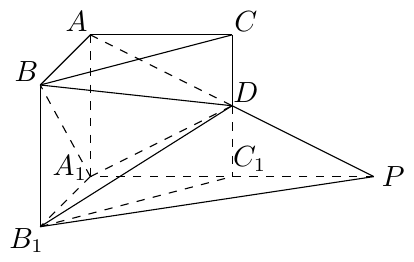
\includegraphics[width=3.4cm]{GaoKao/images/2011/sichuan_science/q19_fig1.png}
\end{center}

        \item 设 \(d\) 为非零实数，\(a_{n} = \frac{1}{n}\left[\mathrm{C}_{n}^{1}d + 2\mathrm{C}_{n}^{2}d^{2} + \dots + (n - 1)\mathrm{C}_{n}^{n - 1}d^{n - 1} + n\mathrm{C}_{n}^{n}d^{n}\right]\) （\(n\in \mathbf{N}^{*}\)）.
\begin{enumerate}
\item 写出 \(a_1\)，\(a_2\)，\(a_3\) 并判断 \(\{a_n\}\) 是否为等比数列. 若是，给出证明；若不是，说明理由；
\item 设 \( b_n = nda_n \) （\( n \in \mathbf{N}^* \)），求数列 \( \{b_n\} \) 的前 \( n \) 项和 \( S_n \).
\end{enumerate}

        \item 椭圆有两顶点 \(A(-1,0)\)，\(B(1,0)\)，过其焦点 \(F(0,1)\) 的直线 \(l\) 与椭圆交于 \(C\)，\(D\) 两点，并与 \(x\) 轴交于点 \(P\). 直线 \(AC\) 与直线 \(BD\) 交于点 \(Q\).
\begin{enumerate}
\item 当 \(|CD| = \frac{3}{2}\sqrt{2}\) 时，求直线 \(l\) 的方程.
\item 当点 \(P\) 异于 \(A\)，\(B\) 两点时，求证： \(\overrightarrow{OP} \cdot \overrightarrow{OQ}\) 为定值.
\end{enumerate}

\begin{center}
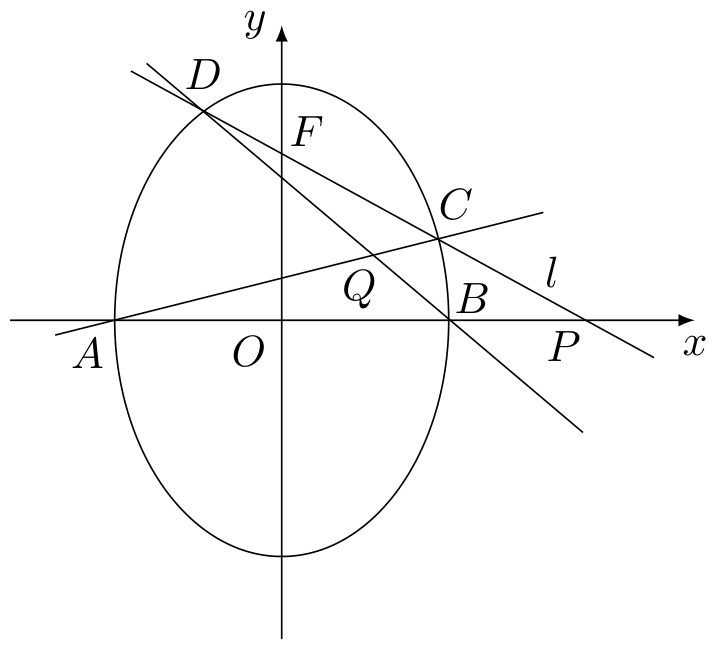
\includegraphics[width=8.9cm]{GaoKao/images/2011/sichuan_science/q21_fig1.png}
\end{center}

        \item 已知函数 \(f(x)=\frac{2}{3}x+\frac{1}{2}\)，\(h(x)=\sqrt{x}\).
\begin{enumerate}
\item 设函数 \(F(x)=f(x)-h(x)\)，求 \(F(x)\) 的单调区间与极值；
\item 设 \(a\in\mathbb{R}\)，解关于 \(x\) 的方程 \(\log_{4}\left[\frac{3}{2}f(x-1)-\frac{3}{4}\right]=\log_{2}h(a-x)-\log_{2}h(4-x)\)；
\item 试比较 \(f(100)h(100)-\displaystyle\sum_{k=1}^{100}h(k)\) 与 \(\frac{1}{6}\) 的大小.
\end{enumerate}

    \end{enumerate}

\end{description}


\subsection{2011年四川卷（文）}\label{gk:2011年四川卷（文）}

\begin{description}

    \item[一、选择题]

    \begin{enumerate}[leftmargin=5pt]

        \item 若全集 \(M = \{1, 2, 3, 4, 5\}\)，\(N = \{2, 4\}\)，则 \(\complement_{M}N =\)（\quad）

        {\centering\begin{tabular*}{\linewidth}{@{}@{\extracolsep{\fill}}llll@{}}
          \text{A. }\(\varnothing\)  &  \text{B. }\(\{1, 3, 5\}\)  &  \text{C. }\(\{2, 4\}\)  &  \text{D. }\(\{1, 2, 3, 4, 5\}\)
        \end{tabular*}\par}

        \item 有一容量为 \(66\) 的样本，数据的分组及各组的频数如下：
\begin{center}
\resizebox{\linewidth}{!}{%
\begin{tabular}{|c|c|c|c|c|c|c|c|}
\hline
\([11.5, 15.5)\) & \([15.5, 19.5)\) & \([19.5, 23.5)\) & \([23.5, 27.5)\) & \([27.5, 31.5)\) & \([31.5, 35.5)\) & \([35.5, 39.5)\) & \([39.5, 43.5)\) \\
\hline
2 & 4 & 9 & 18 & 11 & 12 & 7 & 3 \\
\hline
\end{tabular}%
}
\end{center}
根据样本的频率分布估计，大于或等于 \(31.5\) 的数据约占（\quad）

        {\centering\begin{tabular*}{\linewidth}{@{}@{\extracolsep{\fill}}llll@{}}
          \text{A. }\(\frac{2}{11}\)  &  \text{B. }\(\frac{1}{3}\)  &  \text{C. }\(\frac{1}{2}\)  &  \text{D. }\(\frac{2}{3}\)
        \end{tabular*}\par}

        \item 圆 \(x^2 + y^2 - 4x + 6y = 0\) 的圆心坐标是（\quad）

        {\centering\begin{tabular*}{\linewidth}{@{}@{\extracolsep{\fill}}llll@{}}
          \text{A. }\((2, 3)\)  &  \text{B. }\((-2, 3)\)  &  \text{C. }\((-2, -3)\)  &  \text{D. }\((2, -3)\)
        \end{tabular*}\par}

        \item 函数 \(y = \left(\frac{1}{2}\right)^x + 1\) 的图象关于直线 \(y = x\) 对称的图象大致是（\quad）

        {\centering\begin{tabular*}{\linewidth}{@{}@{\extracolsep{\fill}}cccc@{}}
          \text{A. }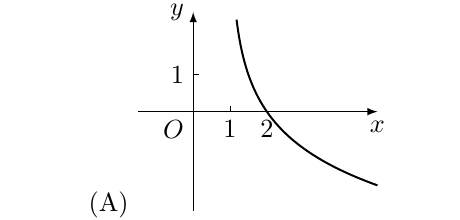
\includegraphics[width=0.15\paperwidth]{GaoKao/images/2011/sichuan_liberal/q4_choice_a.png}  &  \text{B. }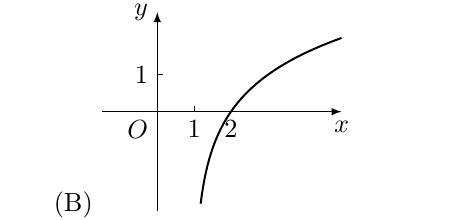
\includegraphics[width=0.15\paperwidth]{GaoKao/images/2011/sichuan_liberal/q4_choice_b.png}  &  \text{C. }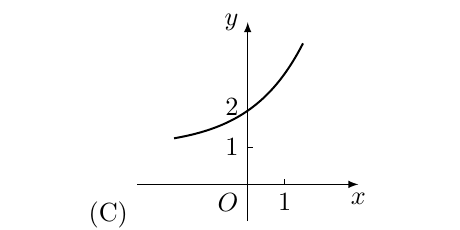
\includegraphics[width=0.15\paperwidth]{GaoKao/images/2011/sichuan_liberal/q4_choice_c.png}  &  \text{D. }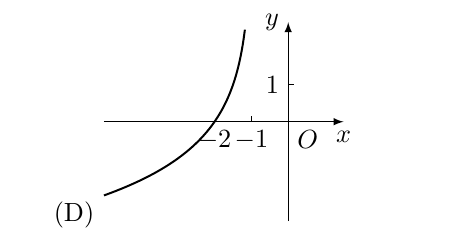
\includegraphics[width=0.15\paperwidth]{GaoKao/images/2011/sichuan_liberal/q4_choice_d.png}
        \end{tabular*}\par}

        \item “\(x = 3\)”是“\(x^2 = 9\)”的（\quad）

        {\centering\begin{tabular*}{\linewidth}{@{}@{\extracolsep{\fill}}llll@{}}
          \text{A. }充分而不必要的条件  &  \text{B. }必要而不充分的条件  &  \text{C. }充要条件  &  \text{D. }既不充分也不必要的条件
        \end{tabular*}\par}

        \item \(l_1\)，\(l_2\)，\(l_3\) 是空间三条不同的直线，则下列命题正确的是（\quad）

        {\centering\begin{tabular*}{\linewidth}{@{}@{\extracolsep{\fill}}llll@{}}
          \text{A. }\(l_1 \perp l_2, l_2 \perp l_3 \Rightarrow l_1 \parallel l_3\)  &  \text{B. }\(l_1 \perp l_2\)，\(l_2 \parallel l_3 \Rightarrow l_1 \perp l_3\)  &  \text{C. }\(l_1 \parallel l_2 \parallel l_3 \Rightarrow l_1\)，\(l_2\)，\(l_3\) 共面  &  \text{D. }\(l_1\)，\(l_2\)，\(l_3\) 共点 \(\Rightarrow l_1\)，\(l_2\)，\(l_3\) 共面
        \end{tabular*}\par}

        \item 如图，正六边形 \(ABCDEF\) 中，\(\overrightarrow{BA} + \overrightarrow{CD} + \overrightarrow{EF} =\)（\quad）

\begin{center}
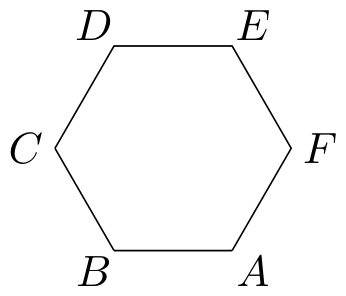
\includegraphics[width=4.3cm]{GaoKao/images/2011/sichuan_liberal/q7_fig1.png}
\end{center}

        {\centering\begin{tabular*}{\linewidth}{@{}@{\extracolsep{\fill}}llll@{}}
          \text{A. }\(0\)  &  \text{B. }\(\overrightarrow{BE}\)  &  \text{C. }\(\overrightarrow{AD}\)  &  \text{D. }\(\overrightarrow{CF}\)
        \end{tabular*}\par}

        \item 在 \(\triangle ABC\) 中，\(\sin^2 A \leqslant \sin^2 B + \sin^2 C - \sin B \sin C\)，则 \(A\) 的取值范围是（\quad）

        {\centering\begin{tabular*}{\linewidth}{@{}@{\extracolsep{\fill}}llll@{}}
          \text{A. }\((0, \frac{\pi}{6}]\)  &  \text{B. }\([\frac{\pi}{6}, \pi)\)  &  \text{C. }\((0, \frac{\pi}{3}]\)  &  \text{D. }\([\frac{\pi}{3}, \pi)\)
        \end{tabular*}\par}

        \item 数列 \(\{a_n\}\) 的前 \(n\) 项和为 \(S_n\)，若 \(a_1 = 1\)，\(a_{n+1} = 3S_n\)（\(n \geqslant 1\)），则 \(a_6 =\)（\quad）

        {\centering\begin{tabular*}{\linewidth}{@{}@{\extracolsep{\fill}}llll@{}}
          \text{A. }\(3 \times 4^4\)  &  \text{B. }\(3 \times 4^4 + 1\)  &  \text{C. }\(4^5\)  &  \text{D. }\(4^5 + 1\)
        \end{tabular*}\par}

        \item 某运输公司有 \(12\) 名驾驶员和 \(19\) 名工人，有 \(8\) 辆载重量为 \(10\text{ 吨}\) 的甲型卡车和 \(7\) 辆载重量为 \(6\text{ 吨}\) 的乙型卡车. 某天需运往 \(A\) 地至少 \(72\text{ 吨}\) 的货物，派用的每辆车需载满且只运送一次，派用的每辆甲型卡车需配 \(2\) 名工人，运送一次可得利润 \(450\text{ 元}\)；派用的每辆乙型卡车需配 \(1\) 名工人，运送一次可得利润 \(350\text{ 元}\)，该公司合理计划当天派用甲、乙卡车的车辆数，可得最大利润 \(z =\)（\quad）

        {\centering\begin{tabular*}{\linewidth}{@{}@{\extracolsep{\fill}}llll@{}}
          \text{A. }\(4650\text{ 元}\)  &  \text{B. }\(4700\text{ 元}\)  &  \text{C. }\(4900\text{ 元}\)  &  \text{D. }\(5000\text{ 元}\)
        \end{tabular*}\par}

        \item 在抛物线 \(y = x^2 + ax - 5\)（\(a \neq 0\)） 上取横坐标为 \(x_1 = -4\)，\(x_2 = 2\) 的两点，经过两点引一条割线，有平行于该割线的一条直线同时与抛物线和圆 \(5x^2 + 5y^2 = 36\) 相切，则抛物线顶点的坐标为（\quad）

        {\centering\begin{tabular*}{\linewidth}{@{}@{\extracolsep{\fill}}llll@{}}
          \text{A. }\((-2, -9)\)  &  \text{B. }\((0, -5)\)  &  \text{C. }\((2, -9)\)  &  \text{D. }\((1, -6)\)
        \end{tabular*}\par}

        \item 在集合 \(\{1, 2, 3, 4, 5\}\) 中任取一个偶数 \(a\) 和一个奇数 \(b\) 构成以原点为起点的向量 \(\alpha = (a, b)\). 从所有得到的以原点为起点的向量中任取两个向量为邻边作平行四边形，记所有作成的平行四边形的个数为 \(n\)，其中面积等于 2 的平行四边形的个数为 \(m\)，则 \(\frac{m}{n} =\)（\quad）

        {\centering\begin{tabular*}{\linewidth}{@{}@{\extracolsep{\fill}}llll@{}}
          \text{A. }\(\frac{2}{15}\)  &  \text{B. }\(\frac{1}{5}\)  &  \text{C. }\(\frac{4}{15}\)  &  \text{D. }\(\frac{1}{3}\)
        \end{tabular*}\par}

    \end{enumerate}

\end{description}

\begin{description}

    \item[二、填空题]

    \begin{enumerate}[leftmargin=5pt]

      \addtocounter{enumi}{+12}

        \item \((x + 1)^9\) 的展开式中 \(x^3\) 的系数是\rule[-0.3ex]{3em}{0.4pt}（用数字作答）

        \item 双曲线 \(\frac{x^2}{64} - \frac{y^2}{36} = 1\) 上一点 \(P\) 到双曲线右焦点的距离是 \(4\)，那么点 \(P\) 到左准线的距离是\rule[-0.3ex]{3em}{0.4pt}.

        \item 如图，半径为 \(4\) 的球 \(O\) 中有一内接圆柱. 当圆柱的侧面积最大时，球的表面积与该圆柱的侧面积之差是\rule[-0.3ex]{3em}{0.4pt}.

\begin{center}
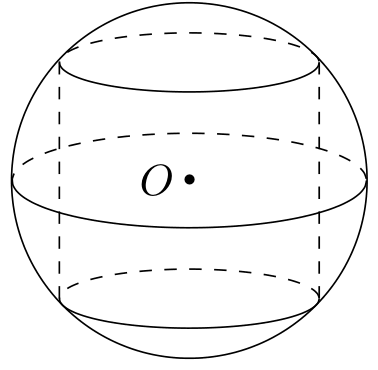
\includegraphics[width=3.4cm]{GaoKao/images/2011/sichuan_liberal/q15_fig1.png}
\end{center}

        \item 函数 \(f(x)\) 的定义域为 \(A\)，若 \(x_1\)，\(x_2 \in A\) 且 \(f(x_1) = f(x_2)\) 时总有 \(x_1 = x_2\)，则称 \(f(x)\) 为单函数. 例如，函数 \(f(x) = 2x + 1\)（\(x \in \mathbb{R}\)）是单函数. 下列命题：

\begin{enumerate}
\item \(f(x) = x^2\)（\(x \in \mathbb{R}\)）是单函数；
\item \(f(x) = 2^x\)（\(x \in \mathbb{R}\)）是单函数；
\item 若 \(f(x)\) 为单函数，\(x_1\)，\(x_2 \in A\) 且 \(x_1 \neq x_2\)，则 \(f(x_1) \neq f(x_2)\)；
\item 在定义域上具有单调性的函数一定是单函数.
\end{enumerate}

其中的真命题是\rule[-0.3ex]{3em}{0.4pt}.（写出所有真命题的编号）

    \end{enumerate}

\end{description}

\begin{description}

    \item[三、解答题]

    \begin{enumerate}[leftmargin=5pt]

      \addtocounter{enumi}{+16}

        \item 本着健康、低碳的生活理念，租自行车骑游的人越来越多. 某自行车租车点的收费标准是每车每次租车时间不超过两小时免费，超过两小时的部分每小时收费 \(2\text{ 元}\)（不足 \(1\) 小时的部分按 \(1\) 小时计算）. 有甲、乙两人相互独立来该租车点租车骑游（各租一车一次）. 设甲、乙不超过两小时还车的概率分别为 \(\frac{1}{4}\)，\(\frac{1}{2}\)；两小时以上且不超过三小时还车的概率分别为 \(\frac{1}{2}\)，\(\frac{1}{4}\)；两人租车时间都不会超过四小时.
\begin{enumerate}
\item 分别求出甲、乙在三小时以上且不超过四小时还车的概率；
\item 求甲、乙两人所付的租车费用之和小于 \(6\text{ 元}\) 的概率.
\end{enumerate}

        \item 已知函数 \(f(x) = \sin \left( x + \frac{7\pi}{4} \right) + \cos \left( x - \frac{3\pi}{4} \right)\)，\(x \in \mathbb{R}\).
\begin{enumerate}
\item 求 \(f(x)\) 的最小正周期和最小值；
\item 已知 \(\cos(\beta - \alpha) = \frac{4}{5}\)，\(\cos(\beta + \alpha) = -\frac{4}{5}\)，\(0 < \alpha < \beta \leqslant \frac{\pi}{2}\)，求证：\([f(\beta)]^2 - 2 = 0\).
\end{enumerate}

        \item 如图，在直三棱柱 \(ABC - A_{1}B_{1}C_{1}\) 中，\(\angle BAC = 90^{\circ}\)，\(AB = AC = AA_{1} = 1\). \(D\) 是棱 \(CC_{1}\) 上的一点，\(P\) 是 \(AD\) 的延长线与 \(A_{1}C_{1}\) 的延长线的交点，且 \(PB_{1} \parallel\) 平面 \(BDA_{1}\).
\begin{enumerate}
\item 求证：\(CD = C_{1}D\)；
\item 求二面角 \(A - A_{1}D - B\) 的平面角的余弦值；
\end{enumerate}
\begin{center}
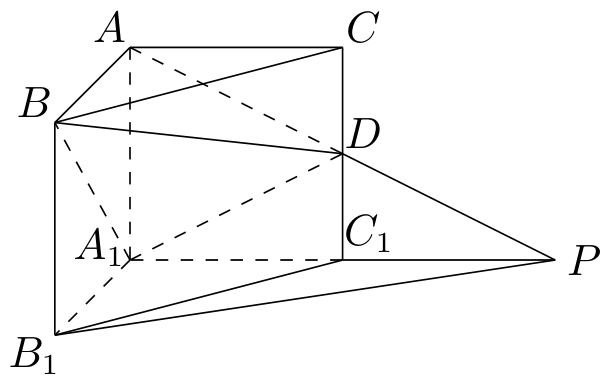
\includegraphics[width=6.3cm]{GaoKao/images/2011/sichuan_liberal/q19_fig1.png}
\end{center}

        \item 已知 \(\{a_n\}\) 是以 \(a\) 为首项，\(q\) 为公比的等比数列，\(S_n\) 为它的前 \(n\) 项和.
\begin{enumerate}
\item 当 \(S_1\)，\(S_3\)，\(S_4\) 成等差数列时，求 \(q\) 的值；
\item 当 \(S_m\)，\(S_n\)，\(S_l\) 成等差数列时，求证：对任意自然数 \(k\)，\(a_{m+k}\)，\(a_{n+k}\)，\(a_{l+k}\) 也成等差数列.
\end{enumerate}

        \item 过点 \(C(0, 1)\) 的椭圆 \(\frac{x^2}{a^2} + \frac{y^2}{b^2} = 1\)（\(a > b > 0\)） 的离心率为 \(\frac{\sqrt{3}}{2}\)，椭圆与 \(x\) 轴交于两点 \(A(a, 0)\)，\(B(-a, 0)\)，过点 \(C\) 的直线 \(l\) 与椭圆交于另一点 \(D\)，并与 \(x\) 轴交于点 \(P\)，直线 \(AC\) 与直线 \(BD\) 交于点 \(Q\).
\begin{enumerate}
\item 当直线 \(l\) 过椭圆右焦点时，求线段 \(CD\) 的长；
\item 当点 \(P\) 异于点 \(B\) 时，求证：\(\overrightarrow{OP} \cdot \overrightarrow{OQ}\) 为定值.
\end{enumerate}
\begin{center}
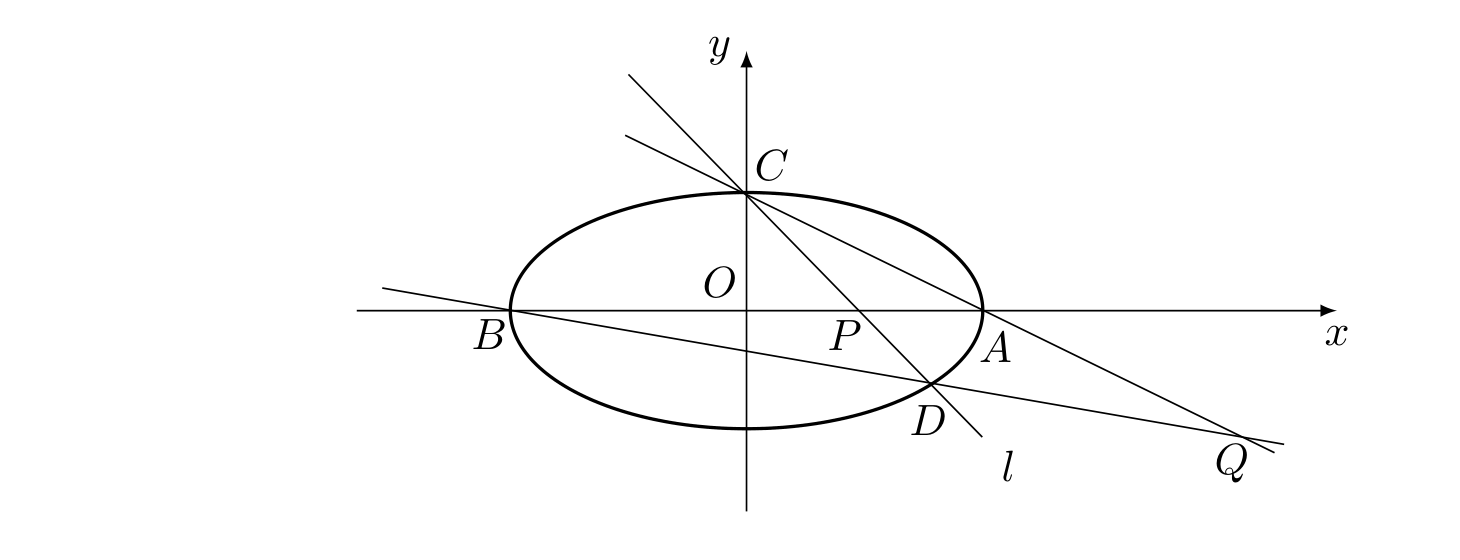
\includegraphics[width=0.90\linewidth]{GaoKao/images/2011/sichuan_liberal/q21_fig1.png}
\end{center}

        \item 已知函数 \(f(x) = \frac{2}{3}x + \frac{1}{2}\)，\(h(x) = \sqrt{x}\).
\begin{enumerate}
\item 设函数 \(F(x) = 18f(x) - x^2[h(x)]^2\)，求 \(F(x)\) 的单调区间与极值；
\item 设 \(a \in \mathbb{R}\)，解关于 \(x\) 的方程 \(\lg \left[ \frac{3}{2}f(x - 1) - \frac{3}{4} \right] = 2\lg h(a - x) - 2\lg h(4 - x)\)；
\item 设 \(n \in \mathbb{N}^{*}\)，证明：\(f(n)h(n) - [h(1) + h(2) + \cdots + h(n)] \geqslant \frac{1}{6}\).
\end{enumerate}

    \end{enumerate}

\end{description}


\subsection{2011年山东卷（理）}\label{gk:2011年山东卷（理）}

\begin{description}

    \item[一、选择题]

    \begin{enumerate}[leftmargin=5pt]

        \item 设集合 \(M = \{x \mid x^2 + x - 6 < 0\}\)，\(N = \{x \mid 1 \leqslant x \leqslant 3\}\). 则 \(M \cap N =\)（\quad）

        {\centering\begin{tabular*}{\linewidth}{@{}@{\extracolsep{\fill}}llll@{}}
          \text{A. }\([1, 2)\)  &  \text{B. }\([1, 2]\)  &  \text{C. }\((2, 3]\)  &  \text{D. }\([2, 3]\)
        \end{tabular*}\par}

        \item 复数 \(z = \frac{2 - \i}{2 + \i}\)（\(\i\) 为虚数单位）在复平面内对应的点所在的象限为（\quad）

        {\centering\begin{tabular*}{\linewidth}{@{}@{\extracolsep{\fill}}llll@{}}
          \text{A. }第一象限  &  \text{B. }第二象限  &  \text{C. }第三象限  &  \text{D. }第四象限
        \end{tabular*}\par}

        \item 若点 \((a,9)\) 在函数 \(y = 3^{x}\) 的图象上，则 \(\tan \frac{a\pi}{6}\) 的值为（\quad）

        {\centering\begin{tabular*}{\linewidth}{@{}@{\extracolsep{\fill}}llll@{}}
          \text{A. }0  &  \text{B. }\( \frac{\sqrt{3}}{3} \)  &  \text{C. }1  &  \text{D. }\(\sqrt{3}\)
        \end{tabular*}\par}

        \item 不等式 \( |x - 5| + |x + 3| \geqslant 10 \) 的解集是（\quad）

        {\centering\begin{tabular*}{\linewidth}{@{}@{\extracolsep{\fill}}llll@{}}
          \text{A. }\([-5,7]\)  &  \text{B. }\([-4,6]\)  &  \text{C. }\((- \infty, -5] \cup [7, +\infty)\)  &  \text{D. }\((- \infty, -4] \cup [6, +\infty)\)
        \end{tabular*}\par}

        \item 对于函数 \(y = f(x)\)，\(x \in \mathbb{R}\). “\( y = |f(x)| \) 的图象关于 \( y \) 轴对称”是“\( y = f(x) \) 是奇函数”的（\quad）

        {\centering\begin{tabular*}{\linewidth}{@{}@{\extracolsep{\fill}}llll@{}}
          \text{A. }充分而不必要条件  &  \text{B. }必要而不充分条件  &  \text{C. }充要条件  &  \text{D. }既不充分也不必要条件
        \end{tabular*}\par}

        \item 若函数 \( f(x) = \sin \omega x \)（\(\omega > 0\)）在区间 \(\left[0, \frac{\pi}{3}\right]\) 上单调递增，在区间 \(\left[\frac{\pi}{3}, \frac{\pi}{2}\right]\) 上单调递减，则 \(\omega =\)（\quad）

        {\centering\begin{tabular*}{\linewidth}{@{}@{\extracolsep{\fill}}llll@{}}
          \text{A. }3  &  \text{B. }2  &  \text{C. }\(\frac{3}{2}\)  &  \text{D. }\(\frac{2}{3}\)
        \end{tabular*}\par}

        \item 某产品的广告费用 \(x\) 与销售额 \(y\) 的统计数据如下表：

\begin{center}
\begin{tabular}{c|cccc}
广告费用 \(x\) （万元） & 4 & 2 & 3 & 5 \\
\hline
销售额 \(y\) （万元） & 49 & 26 & 39 & 54
\end{tabular}
\end{center}

根据上表可得回归方程 \( \hat{y} = \hat{b}x + \hat{a} \) 中的 \(\hat{b}\) 为 \(9.4\)，据此模型预报广告费用为 \(6\text{ 万元}\) 时销售额为（\quad）

        {\centering\begin{tabular*}{\linewidth}{@{}@{\extracolsep{\fill}}llll@{}}
          \text{A. }\(63.6\text{ 万元}\)  &  \text{B. }\(65.5\text{ 万元}\)  &  \text{C. }\(67.7\text{ 万元}\)  &  \text{D. }\(72.0\text{ 万元}\)
        \end{tabular*}\par}

        \item 已知双曲线 \(\frac{x^2}{a^2} - \frac{y^2}{b^2} = 1 \) （\(a > 0, b > 0\)）的两条渐近线均和圆 \(C: x^2 + y^2 - 6x + 5 = 0\) 相切，且双曲线右焦点为圆 \(C\) 的圆心，则该双曲线的方程为（\quad）

        {\centering\begin{tabular*}{\linewidth}{@{}@{\extracolsep{\fill}}llll@{}}
          \text{A. }\(\frac{x^2}{5} -\frac{y^2}{4} = 1\)  &  \text{B. }\(\frac{x^2}{4} -\frac{y^2}{5} = 1\)  &  \text{C. }\(\frac{x^2}{3} -\frac{y^2}{6} = 1\)  &  \text{D. }\(\frac{x^2}{6} -\frac{y^2}{3} = 1\)
        \end{tabular*}\par}

        \item 函数 \( y = \frac{x}{2} - 2\sin x \) 的图象大致是（\quad）

        {\centering\begin{tabular*}{\linewidth}{@{}@{\extracolsep{\fill}}cccc@{}}
          \text{A. }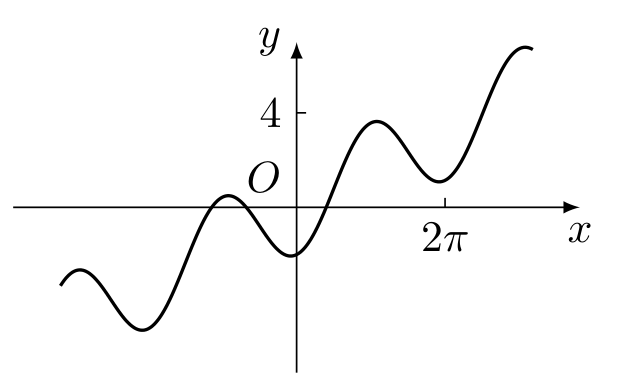
\includegraphics[width=0.15\paperwidth]{GaoKao/images/2011/shandong_science/q9_choice_a.png}  &  \text{B. }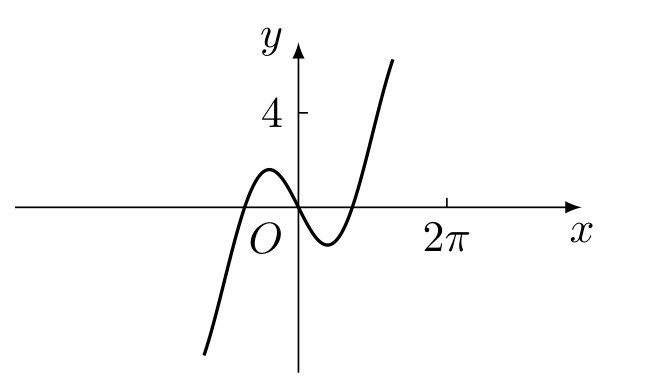
\includegraphics[width=0.15\paperwidth]{GaoKao/images/2011/shandong_science/q9_choice_b.png}  &  \text{C. }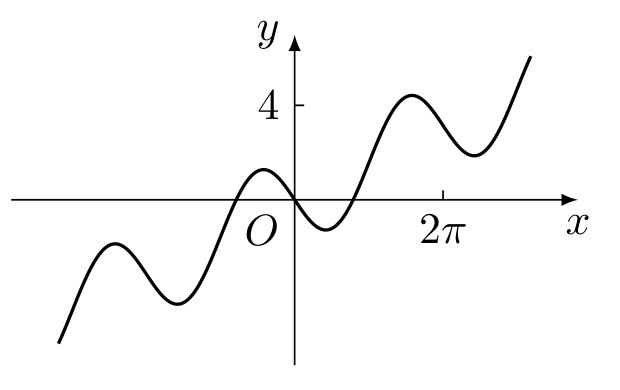
\includegraphics[width=0.15\paperwidth]{GaoKao/images/2011/shandong_science/q9_choice_c.png}  &  \text{D. }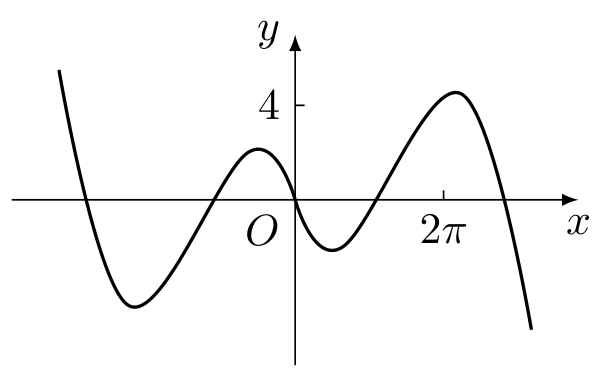
\includegraphics[width=0.15\paperwidth]{GaoKao/images/2011/shandong_science/q9_choice_d.png}
        \end{tabular*}\par}

        \item 已知 \( f(x) \) 是 \( \mathbb{R} \) 上最小正周期为 2 的周期函数，且当 \( 0 \leqslant x < 2 \) 时，\( f(x) = x^3 - x \)，则函数 \( y = f(x) \) 的图象在区间 \([0, 6]\) 上与 \( x \) 轴的交点的个数为（\quad）

        {\centering\begin{tabular*}{\linewidth}{@{}@{\extracolsep{\fill}}llll@{}}
          \text{A. }6  &  \text{B. }7  &  \text{C. }8  &  \text{D. }9
        \end{tabular*}\par}

        \item 如图是长和宽分别相等的两个矩形. 给定下列三个命题：

\begin{enumerate}
\item 存在三棱柱，其正（主）视图，俯视图如图；
\item 存在四棱柱，其正（主）视图，俯视图如图；
\item 存在圆柱，其正（主）视图，俯视图如图.
\end{enumerate}

其中真命题的个数是（\quad）
\begin{center}

\includegraphics[width=5.6cm]{GaoKao/images/2011/shandong_science/q11_fig1.png}
\end{center}

        {\centering\begin{tabular*}{\linewidth}{@{}@{\extracolsep{\fill}}llll@{}}
          \text{A. }3  &  \text{B. }2  &  \text{C. }1  &  \text{D. }0
        \end{tabular*}\par}

        \item 设 \(A_{1}\)，\(A_{2}\)，\(A_{3}\)，\(A_{4}\) 是平面直角坐标系中两两不同的四点. 若 \(\overrightarrow{A_{1}A_{3}} = \lambda \overrightarrow{A_{1}A_{2}}\) （\(\lambda \in \mathbb{R}\)），\(\overrightarrow{A_{1}A_{4}} = \mu \overrightarrow{A_{1}A_{2}}\) （\(\mu \in \mathbb{R}\)），且 \(\frac{1}{\lambda} + \frac{1}{\mu} = 2\)，则称 \(A_{3}\)，\(A_{4}\) 调和分割 \(A_{1}\)，\(A_{2}\). 已知平面上的点 \(C\)，\(D\) 调和分割点 \(A\)，\(B\)，则下面说法正确的是（\quad）

        {\centering\begin{tabular*}{\linewidth}{@{}@{\extracolsep{\fill}}llll@{}}
          \text{A. }\(C\) 可能是线段 \(AB\) 的中点  &  \text{B. }\(D\) 可能是线段 \(AB\) 的中点  &  \text{C. }\(C\)，\(D\) 可能同时在线段 \(AB\) 上  &  \text{D. }\(C\)，\(D\) 不可能同时在线段 \(AB\) 的延长线上
        \end{tabular*}\par}

    \end{enumerate}

\end{description}

\begin{description}

    \item[二、填空题]

    \begin{enumerate}[leftmargin=5pt]

      \addtocounter{enumi}{+12}

        \item 执行如图所示的程序框图，输入 \(l = 2\)，\(m = 3\)，\(n = 5\)，则输出的 \(y\) 的值是\rule[-0.3ex]{3em}{0.4pt}.

\begin{center}
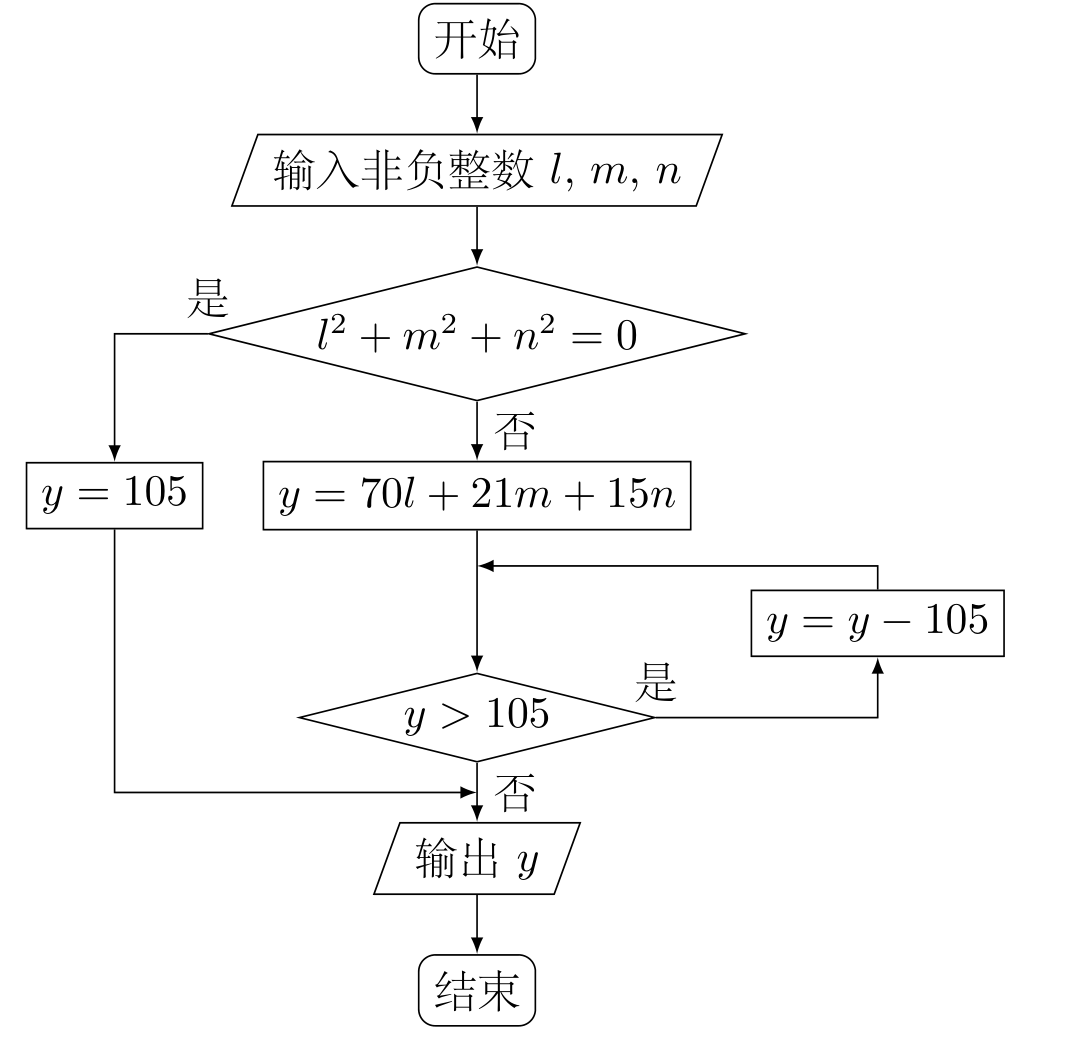
\includegraphics[width=6.5cm]{GaoKao/images/2011/shandong_science/q13_fig1.png}
\end{center}

        \item 若 \(\left(x - \frac{\sqrt{a}}{x^{2}}\right)^6\) 展开式的常数项为 60，则常数 \(a\) 的值为\rule[-0.3ex]{3em}{0.4pt}.

        \item 设函数 \(f(x) = \frac{x}{x + 2}\)（\(x > 0\)），观察：\(f_{1}(x) = f(x) = \frac{x}{x + 2}\)，\(f_{2}(x) = f\!\left(f_{1}(x)\right) = \frac{x}{3x + 4}\)，\(f_{3}(x) = f\!\left(f_{2}(x)\right) = \frac{x}{7x + 8}\)，\(f_{4}(x) = f\!\left(f_{3}(x)\right) = \frac{x}{15x + 16}\). 根据以上事实，由归纳推理可得：当 \(n \in \mathbb{N}^{*}\) 且 \(n \geqslant 2\) 时，\(f_n(x) = f(f_{n-1}(x)) =\)\rule[-0.3ex]{3em}{0.4pt}.

        \item 已知函数 \( f(x) = \log_a x + x - b \)（\(a > 0\)，且 \(a \neq 1\)）. 当 \( 2 < a < 3 < b < 4 \) 时，函数 \( f(x) \) 的零点 \(x_0 \in (n, n+1)\)，\(n \in \mathbb{N}^{*}\)，则 \( n = \)\rule[-0.3ex]{3em}{0.4pt}.

    \end{enumerate}

\end{description}

\begin{description}

    \item[三、解答题]

    \begin{enumerate}[leftmargin=5pt]

      \addtocounter{enumi}{+16}

        \item 在 \(\triangle ABC\) 中，内角 \(A\)，\(B\)，\(C\) 的对边分别为 \(a\)，\(b\)，\(c\)，已知 \(\frac{\cos A - 2 \cos C}{\cos B} = \frac{2c - a}{b}\).
\begin{enumerate}
\item 求 \(\frac{\sin C}{\sin A}\) 的值；
\item 若 \(\cos B = \frac{1}{4}\)，\(b = 2\)，求 \(\triangle ABC\) 的面积 \(S\).
\end{enumerate}

        \item 红队队员甲，乙，丙与蓝队队员 \(A\)，\(B\)，\(C\) 进行围棋比赛，甲对 \(A\)，乙对 \(B\)，丙对 \(C\) 各一盘. 已知甲胜 \(A\)，乙胜 \(B\)，丙胜 \(C\) 的概率分别为 \(0.6\)，\(0.5\)，\(0.5\). 假设各盘比赛结果相互独立.
\begin{enumerate}
\item 求红队至少两名队员获胜的概率；
\item 用 \(\xi\) 表示红队队员获胜的总数，求 \(\xi\) 的分布列和数学期望 \(E(\xi)\).
\end{enumerate}

        \item 在如图所示的几何体中，四边形 \(ABCD\) 为平行四边形，\(\angle ACB = 90^{\circ}\)，\(EA \perp\) 平面 \(ABCD\)，\(EF \parallel AB\)，\(FG \parallel BC\)，\(EG \parallel AC\)，\(AB = 2EF\).
\begin{enumerate}
\item 若 \(M\) 是线段 \(AD\) 的中点，求证：\(GM \parallel\) 平面 \(ABFE\)；
\item 若 \(AC = BC = 2AE\)，求二面角 \(A - BF - C\) 的大小.
\end{enumerate}

\begin{center}
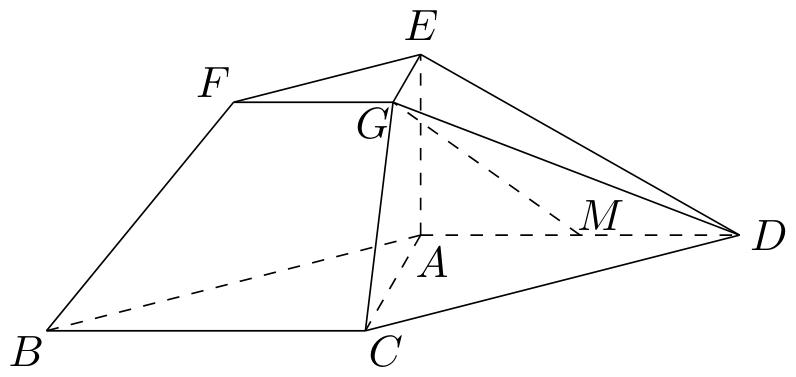
\includegraphics[width=9.9cm]{GaoKao/images/2011/shandong_science/q19_fig1.png}
\end{center}

        \item 等比数列 \(\{a_{n}\}\) 中，\(a_{1}\)，\(a_{2}\)，\(a_{3}\) 分别是下表第一，二，三行中的某一个数，且 \(a_{1}\)，\(a_{2}\)，\(a_{3}\) 中的任何两个数不在下表的同一列.

\begin{center}
\begin{tabular}{c|ccc}
 & 第一列 & 第二列 & 第三列 \\
\hline
第一行 & 3 & 2 & 10 \\
第二行 & 6 & 4 & 14 \\
第三行 & 9 & 8 & 18
\end{tabular}
\end{center}

\begin{enumerate}
\item 求数列 \(\{a_{n}\}\) 的通项公式；
\item 若数列 \(\{b_{n}\}\) 满足： \(b_{n} = a_{n} + (-1)^{n} \ln a_{n}\)，求数列 \(\{b_{n}\}\) 的前 \(n\) 项和 \(S_{n}\).
\end{enumerate}

        \item 某企业拟建造如图所示的容器（不计厚度，长度单位：米），其中容器的中间为圆柱形，左右两端均为半球形，按照设计要求容器的容积为 \(\frac{80\pi}{3}\text{ 立方米}\)，且 \(l\geqslant2r\). 假设该容器的建造费用仅与其表面积有关. 已知圆柱形部分每平方米建造费用为 \(3\text{ 千元}\)，半球形部分每平方米建造费用为 \(c\text{ 千元}\)（\(c>3\)）. 设该容器的建造费用为 \(y\text{ 千元}\).
\begin{enumerate}
\item 写出 \(y\) 关于 \(r\) 的函数表达式，并求该函数的定义域；
\item 求该容器的建造费用最小时的 \(r\).
\end{enumerate}

\begin{center}
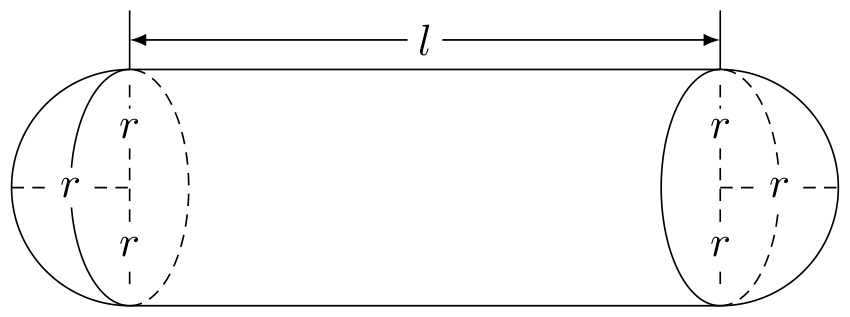
\includegraphics[width=15.5cm]{GaoKao/images/2011/shandong_science/q21_fig1.png}
\end{center}

        \item 已知动直线 \(l\) 与椭圆 \(C: \frac{x^2}{3} + \frac{y^2}{2} = 1\) 交于 \(P(x_1, y_1)\)，\(Q(x_2, y_2)\) 两不同点，且 \(\triangle OPQ\) 的面积 \(S_{\triangle OPQ} = \frac{\sqrt{6}}{2}\). 其中 \(O\) 为坐标原点.
\begin{enumerate}
\item 证明： \(x_1^2 + x_2^2\) 和 \(y_1^2 + y_2^2\) 均为定值；
\item 设线段 \(PQ\) 的中点为 \(M\)，求 \(|OM| \cdot |PQ|\) 的最大值；
\item 椭圆 \(C\) 上是否存在三点 \(D\)，\(E\)，\(G\)，使得 \(S_{\triangle DOE} = S_{\triangle ODG} = S_{\triangle OEG} = \frac{\sqrt{6}}{2}\)；若存在，判断 \(\triangle DEG\) 的形状；若不存在，请说明理由.
\end{enumerate}

    \end{enumerate}

\end{description}


\subsection{2011年山东卷（文）}\label{gk:2011年山东卷（文）}

\begin{description}

    \item[一、选择题]

    \begin{enumerate}[leftmargin=5pt]

        \item 设集合 \(M = \{x \mid (x + 3)(x - 2) < 0\}\)，\(N = \{x \mid 1 \leqslant x \leqslant 3\}\)，则 \(M \cap N =\)（\quad）

        {\centering\begin{tabular*}{\linewidth}{@{}@{\extracolsep{\fill}}llll@{}}
          \text{A. }\([1,2)\)  &  \text{B. }\([1,2]\)  &  \text{C. }\((2,3]\)  &  \text{D. }\([2,3]\)
        \end{tabular*}\par}

        \item 复数 \(z = \frac{2 - \i}{2 + \i}\)（\(\i\) 为虚数单位）在复平面内对应的点所在的象限为（\quad）

        {\centering\begin{tabular*}{\linewidth}{@{}@{\extracolsep{\fill}}llll@{}}
          \text{A. }第一象限  &  \text{B. }第二象限  &  \text{C. }第三象限  &  \text{D. }第四象限
        \end{tabular*}\par}

        \item 若点 \((a,9)\) 在函数 \(y = 3^{x}\) 的图象上，则 \(\tan \frac{a\pi}{6}\) 的值为（\quad）

        {\centering\begin{tabular*}{\linewidth}{@{}@{\extracolsep{\fill}}llll@{}}
          \text{A. }0  &  \text{B. }\(\frac{\sqrt{3}}{3}\)  &  \text{C. }1  &  \text{D. }\(\sqrt{3}\)
        \end{tabular*}\par}

        \item 曲线 \( y = x^{3} + 11 \) 在点 \( P(1,12) \) 处的切线与 \( y \) 轴交点的纵坐标是（\quad）

        {\centering\begin{tabular*}{\linewidth}{@{}@{\extracolsep{\fill}}llll@{}}
          \text{A. }\(-9\)  &  \text{B. }\(-3\)  &  \text{C. }9  &  \text{D. }15
        \end{tabular*}\par}

        \item 已知 \(a\)，\(b\)，\(c \in \mathbb{R}\)，命题“若 \(a + b + c = 3\)，则 \(a^2 + b^2 + c^2 \geqslant 3\)”的否命题是（\quad）

        {\centering\begin{tabular*}{\linewidth}{@{}@{\extracolsep{\fill}}llll@{}}
          \text{A. }若 \(a + b + c \neq 3\)，则 \(a^2 + b^2 + c^2 < 3\)  &  \text{B. }若 \(a + b + c = 3\)，则 \(a^2 + b^2 + c^2 < 3\)  &  \text{C. }若 \(a + b + c \neq 3\)，则 \(a^2 + b^2 + c^2 \geqslant 3\)  &  \text{D. }若 \(a^2 + b^2 + c^2 \geqslant 3\)，则 \(a + b + c = 3\)
        \end{tabular*}\par}

        \item 若函数 \(f(x) = \sin \omega x\)（\(\omega > 0\)） 在区间 \(\left[0, \frac{\pi}{3}\right]\) 上单调递增，在区间 \(\left[\frac{\pi}{3}, \frac{\pi}{2}\right]\) 上单调递减，则 \(\omega =\)（\quad）

        {\centering\begin{tabular*}{\linewidth}{@{}@{\extracolsep{\fill}}llll@{}}
          \text{A. }\(\frac{2}{3}\)  &  \text{B. }\(\frac{3}{2}\)  &  \text{C. }2  &  \text{D. }3
        \end{tabular*}\par}

        \item 设变量 \(x\)，\(y\) 满足约束条件 \(\begin{cases}
x + 2y - 5 \leqslant 0,\\
x - y - 2 \leqslant 0,\\
x \geqslant 0,
\end{cases}\) 则目标函数 \(z = 2x + 3y + 1\) 的最大值为（\quad）

        {\centering\begin{tabular*}{\linewidth}{@{}@{\extracolsep{\fill}}llll@{}}
          \text{A. }11  &  \text{B. }10  &  \text{C. }9  &  \text{D. }8.5
        \end{tabular*}\par}

        \item 某产品的广告费用 \(x\) 与销售额 \(y\) 的统计数据如下表：

\begin{center}
\begin{tabular}{c|cccc}
广告费用 \(x\)（万元） & 4 & 2 & 3 & 5 \\
\hline
销售额 \(y\)（万元） & 49 & 26 & 39 & 54
\end{tabular}
\end{center}

根据上表可得回归方程 \(\hat{y} = \hat{b}x + \hat{a}\) 中的 \(\hat{b}\) 为 9.4，据此模型预报广告费用为 6 万元时销售额为（\quad）

        {\centering\begin{tabular*}{\linewidth}{@{}@{\extracolsep{\fill}}llll@{}}
          \text{A. }\(63.6\text{ 万元}\)  &  \text{B. }\(65.5\text{ 万元}\)  &  \text{C. }\(67.7\text{ 万元}\)  &  \text{D. }\(72.0\text{ 万元}\)
        \end{tabular*}\par}

        \item 设 \(M(x_0, y_0)\) 为抛物线 \(C: x^2 = 8y\) 上一点，\(F\) 为抛物线 \(C\) 的焦点，以 \(F\) 为圆心，\(|FM|\) 为半径的圆和抛物线 \(C\) 的准线相交，则 \(y_0\) 的取值范围是（\quad）

        {\centering\begin{tabular*}{\linewidth}{@{}@{\extracolsep{\fill}}llll@{}}
          \text{A. }\((0,2)\)  &  \text{B. }\([0,2]\)  &  \text{C. }\((2, + \infty)\)  &  \text{D. }\([2, + \infty)\)
        \end{tabular*}\par}

        \item 函数 \( y = \frac{x}{2} - 2\sin x \) 的图象大致是（\quad）

        {\centering\begin{tabular*}{\linewidth}{@{}@{\extracolsep{\fill}}cccc@{}}
          \text{A. }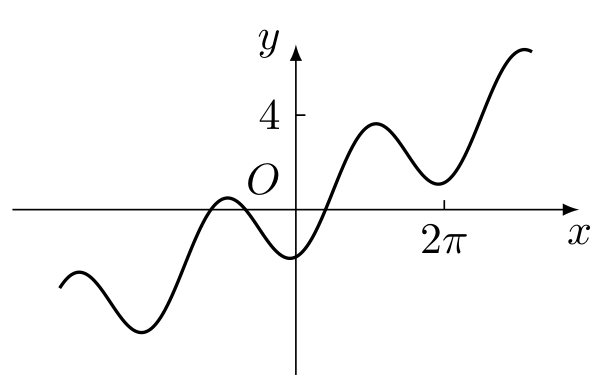
\includegraphics[width=0.15\paperwidth]{GaoKao/images/2011/shandong_liberal/q10_choice_a.png}  &  \text{B. }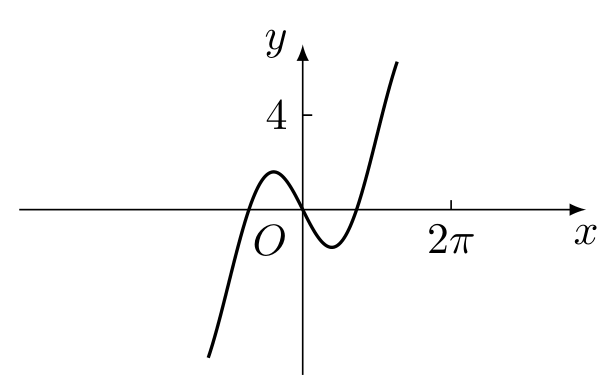
\includegraphics[width=0.15\paperwidth]{GaoKao/images/2011/shandong_liberal/q10_choice_b.png}  &  \text{C. }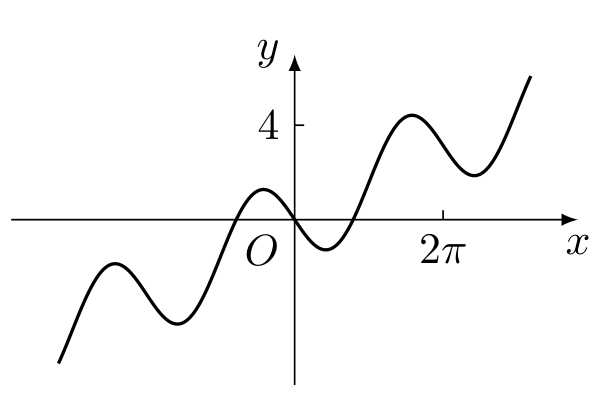
\includegraphics[width=0.15\paperwidth]{GaoKao/images/2011/shandong_liberal/q10_choice_c.png}  &  \text{D. }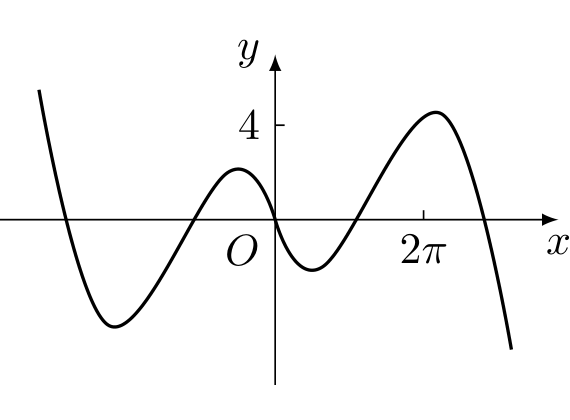
\includegraphics[width=0.15\paperwidth]{GaoKao/images/2011/shandong_liberal/q10_choice_d.png}
        \end{tabular*}\par}

        \item 如图是长和宽分别相等的两个矩形. 给定下列三个命题：
\begin{enumerate}
\item 存在三棱柱，其正（主）视图，俯视图如图；
\item 存在四棱柱，其正（主）视图，俯视图如图；
\item 存在圆柱，其正（主）视图，俯视图如图.
\end{enumerate}
其中真命题的个数是（\quad）

\begin{center}
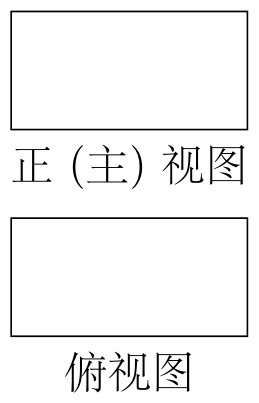
\includegraphics[width=2.5cm]{GaoKao/images/2011/shandong_liberal/q11_fig1.png}
\end{center}

        {\centering\begin{tabular*}{\linewidth}{@{}@{\extracolsep{\fill}}llll@{}}
          \text{A. }3  &  \text{B. }2  &  \text{C. }1  &  \text{D. }0
        \end{tabular*}\par}

        \item 设 \(A_{1}\)，\(A_{2}\)，\(A_{3}\)，\(A_{4}\) 是平面直角坐标系中两两不同的四点，若 \(\overrightarrow{A_{1}A_{3}} = \lambda \overrightarrow{A_{1}A_{2}}\) （\(\lambda \in \mathbb{R}\)），\(\overrightarrow{A_{1}A_{4}} = \mu \overrightarrow{A_{1}A_{2}}\) （\(\mu \in \mathbb{R}\)），且 \(\frac{1}{\lambda} + \frac{1}{\mu} = 2\)，则称 \(A_{3}\)，\(A_{4}\) 调和分割 \(A_{1}\)，\(A_{2}\). 已知点 \(C(c, 0)\)，\(D(d, 0)\) （\(c\)，\(d \in \mathbb{R}\)） 调和分割点 \(A(0, 0)\)，\(B(1, 0)\)，则下面说法正确的是（\quad）

        {\centering\begin{tabular*}{\linewidth}{@{}@{\extracolsep{\fill}}llll@{}}
          \text{A. }\(C\) 可能是线段 \(AB\) 的中点  &  \text{B. }\(D\) 可能是线段 \(AB\) 的中点  &  \text{C. }\(C\)，\(D\) 可能同时在线段 \(AB\) 上  &  \text{D. }\(C\)，\(D\) 不可能同时在线段 \(AB\) 的延长线上
        \end{tabular*}\par}

    \end{enumerate}

\end{description}

\begin{description}

    \item[二、填空题]

    \begin{enumerate}[leftmargin=5pt]

      \addtocounter{enumi}{+12}

        \item 某高校甲，乙，丙，丁四个专业分别有 150，150，400，300 名学生，为了解学生的就业倾向，用分层抽样的方法从该校这四个专业共抽取 40 名学生进行调查，应在丙专业抽取的学生人数为\rule[-0.3ex]{3em}{0.4pt}.

        \item 执行如图所示的程序框图，输入 \(l = 2\)，\(m = 3\)，\(n = 5\)，则输出的 \(y\) 的值是\rule[-0.3ex]{3em}{0.4pt}.

\begin{center}
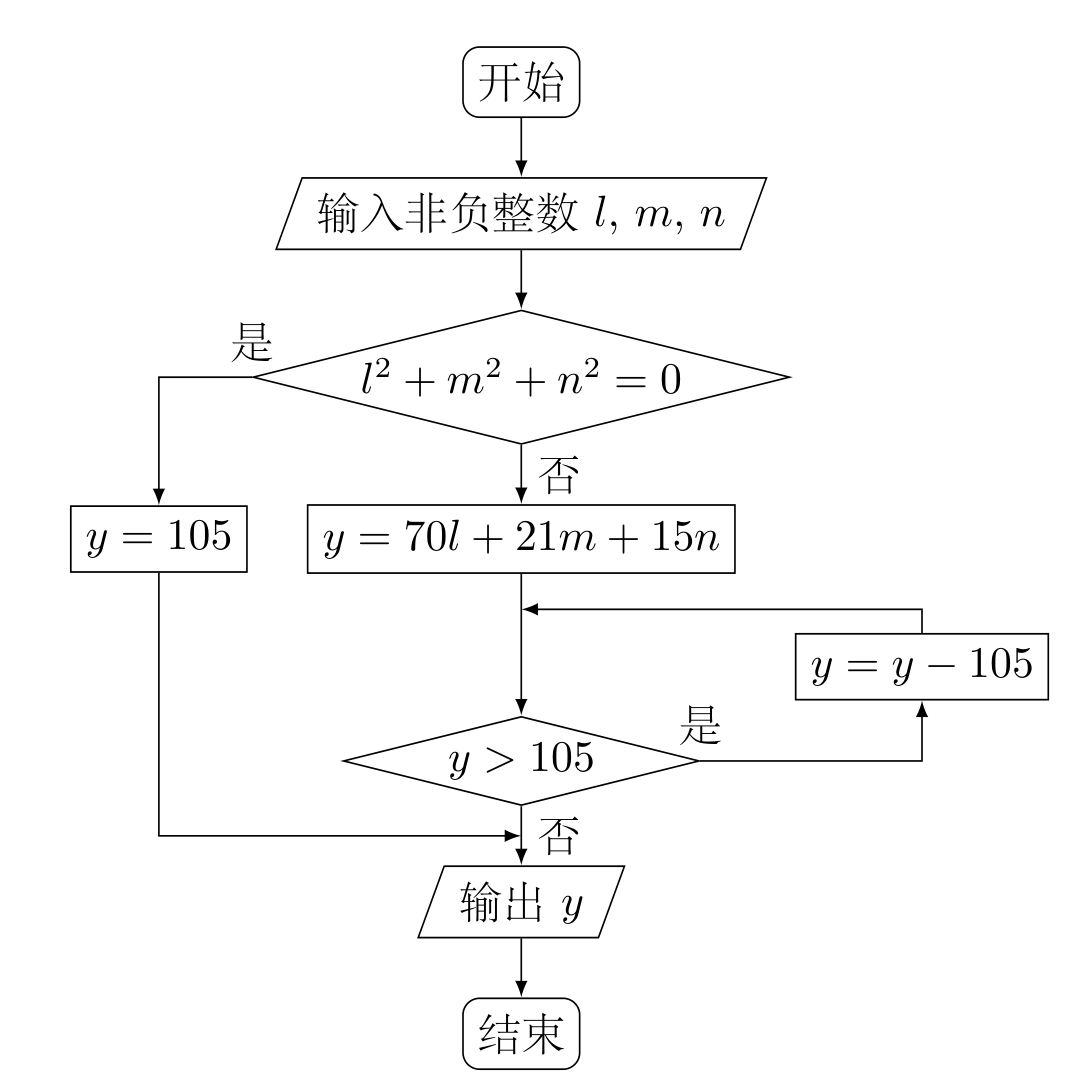
\includegraphics[width=6.8cm]{GaoKao/images/2011/shandong_liberal/q14_fig1.png}
\end{center}

        \item 已知双曲线 \(\frac{x^2}{a^2} - \frac{y^2}{b^2} = 1\)（\(a > 0\)，\(b > 0\)）和椭圆 \(\frac{x^2}{16} + \frac{y^2}{9} = 1\) 有相同的焦点，且双曲线的离心率是椭圆离心率的两倍，则双曲线的方程为\rule[-0.3ex]{3em}{0.4pt}.

        \item 已知函数 \(f(x) = \log_a x + x - b\)（\(a > 0\)，且 \(a \neq 1\)）. 当 \(2 < a < 3 < b < 4\) 时，函数 \(f(x)\) 的零点 \(x_0 \in (n, n + 1)\)，\(n \in \mathbb{N}^*\)，则 \(n = \)\rule[-0.3ex]{3em}{0.4pt}.

    \end{enumerate}

\end{description}

\begin{description}

    \item[三、解答题]

    \begin{enumerate}[leftmargin=5pt]

      \addtocounter{enumi}{+16}

        \item 在 \(\triangle ABC\) 中，内角 \(A\)，\(B\)，\(C\) 的对边分别为 \(a\)，\(b\)，\(c\)，已知 \(\frac{\cos A - 2\cos C}{\cos B} = \frac{2c - a}{b}\).
\begin{enumerate}
\item 求 \( \frac{\sin C}{\sin A} \) 的值；
\item 若 \( \cos B = \frac{1}{4} \)，\( \triangle ABC \) 的周长为 5，求 \(b\) 的长.
\end{enumerate}

        \item 甲，乙两校各有 3 名教师报名支教. 其中甲校 2 男 1 女，乙校 1 男 2 女.
\begin{enumerate}
\item 若从甲校和乙校报名的教师中各任选 1 名，写出所有可能的结果，并求选出的 2 名教师性别相同的概率；
\item 若从报名的 6 名教师中任选 2 名，写出所有可能的结果，并求选出的 2 名教师来自同一学校的概率.
\end{enumerate}

        \item 如图，在四棱台 \(ABCD - A_{1}B_{1}C_{1}D_{1}\) 中，\(D_{1}D \perp\) 平面 \(ABCD\)，底面 \(ABCD\) 是平行四边形，\(AB = 2AD\)，\(AD = A_{1}B_{1}\)，\(\angle BAD = 60^{\circ}\).
\begin{enumerate}
\item 证明： \(AA_{1} \perp BD\).
\item 证明：\(CC_{1} \parallel\) 平面 \(A_{1}BD\).
\end{enumerate}

\begin{center}
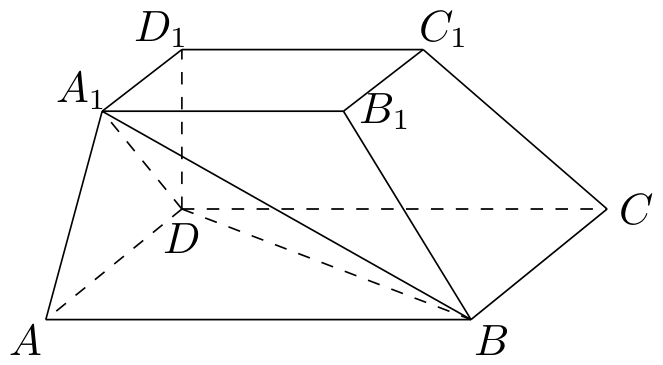
\includegraphics[width=6.8cm]{GaoKao/images/2011/shandong_liberal/q19_fig1.png}
\end{center}

        \item 等比数列 \(\{a_{n}\}\) 中，\(a_{1}\)，\(a_{2}\)，\(a_{3}\) 分别是下表第一、二、三行中的某一个数，且 \(a_{1}\)，\(a_{2}\)，\(a_{3}\) 中的任何两个数不在下表的同一列.

\begin{center}
\begin{tabular}{c|ccc}
 & 第一列 & 第二列 & 第三列 \\
\hline
第一行 & 3 & 2 & 10 \\
第二行 & 6 & 4 & 14 \\
第三行 & 9 & 8 & 18
\end{tabular}
\end{center}

\begin{enumerate}
\item 求数列 \(\{a_{n}\}\) 的通项公式；
\item 若数列 \(\{b_{n}\}\) 满足：\(b_{n}=a_{n}+(-1)^{n}\ln a_{n}\)，求数列 \(\{b_{n}\}\) 的前 \(2n\) 项和 \(S_{2n}\).
\end{enumerate}

        \item 某企业拟建造如图所示的容器（不计厚度，长度单位：米），其中容器的中间为圆柱形，左右两端均为半球形，按照设计要求容器的容积为 \(\frac{80\pi}{3}\) 立方米，且 \(l \geqslant 2r\). 假设该容器的建造费用仅与其表面积有关. 已知圆柱形部分每平方米建造费用为 3 千元，半球形部分每平方米建造费用为 \(c \) （\(c > 3\)）千元. 设该容器的建造费用为 \(y\) 千元.
\begin{enumerate}
\item 写出 \(y\) 关于 \(r\) 的函数表达式，并求该函数的定义域；
\item 求该容器的建造费用最小时的 \(r\).
\end{enumerate}

\begin{center}
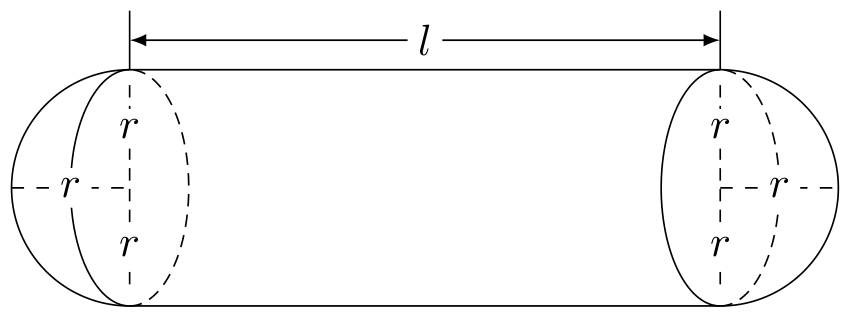
\includegraphics[width=14.2cm]{GaoKao/images/2011/shandong_liberal/q21_fig1.png}
\end{center}

        \item 在平面直角坐标系 \(xOy\) 中，已知椭圆 \(C: \frac{x^2}{3} + y^2 = 1\). 如图所示，斜率为 \(k \) （\(k > 0\)）且不过原点的直线 \(l\) 交椭圆 \(C\) 于 \(A\)，\(B\) 两点. 线段 \(AB\) 的中点为 \(E\). 射线 \(OE\) 交椭圆 \(C\) 于点 \(G\)，交直线 \(x = -3\) 于点 \(D(-3, m)\).
\begin{enumerate}
\item 求 \(m^{2} + k^{2}\) 的最小值；
\item 若 \(\left|OG\right|^{2}=\left|OD\right|\cdot\left|OE\right|\)，
\begin{enumerate}
\item 求证：直线 \(l\) 过定点；
\item 试问点 \(B\)，\(G\) 能否关于 \(x\) 轴对称？若能，求出此时 \(\triangle ABG\) 的外接圆方程. 若不能，请说明理由.
\end{enumerate}
\end{enumerate}

\begin{center}
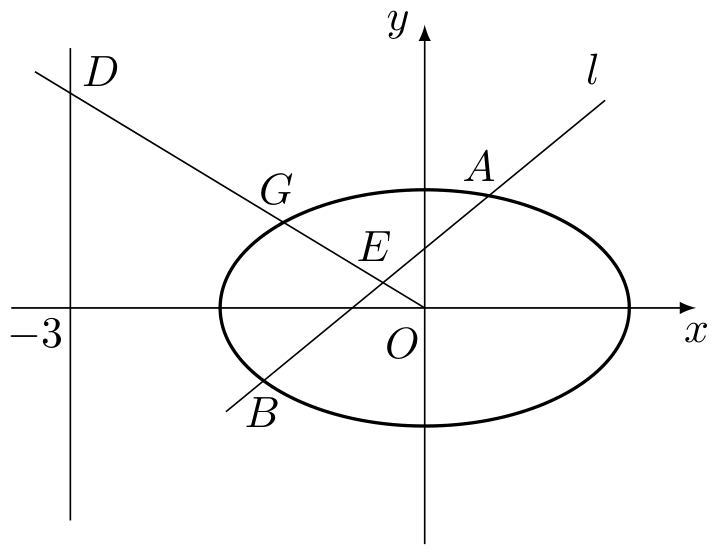
\includegraphics[width=9.5cm]{GaoKao/images/2011/shandong_liberal/q22_fig1.png}
\end{center}

    \end{enumerate}

\end{description}


\subsection{2011年陕西卷（理）}\label{gk:2011年陕西卷（理）}

\begin{description}

    \item[一、选择题]

    \begin{enumerate}[leftmargin=5pt]

        \item 设 \(\bm{a}\)，\(\bm{b}\) 是向量，命题“若 \(\bm{a} = -\bm{b}\)，则 \(|\bm{a}| = |\bm{b}|\)”的逆命题是（\quad）

        {\centering\begin{tabular*}{\linewidth}{@{}@{\extracolsep{\fill}}llll@{}}
          \text{A. }若 \(\bm{a} \neq -\bm{b}\)，则 \(|\bm{a}| \neq |\bm{b}|\).  &  \text{B. }若 \(\bm{a} = -\bm{b}\)，则 \(|\bm{a}| \neq |\bm{b}|\)  &  \text{C. }若 \(|\bm{a}| \neq |\bm{b}|\)，则 \(\bm{a} \neq -\bm{b}\)  &  \text{D. }若 \(|\bm{a}| = |\bm{b}|\)，则 \(\bm{a} = -\bm{b}\)
        \end{tabular*}\par}

        \item 设抛物线的顶点在原点，准线方程为 \(x = -2\)，则抛物线的方程是（\quad）

        {\centering\begin{tabular*}{\linewidth}{@{}@{\extracolsep{\fill}}llll@{}}
          \text{A. }\( y^{2} = -8x \)  &  \text{B. }\( y^{2} = -4x \)  &  \text{C. }\( y^{2} = 8x \)  &  \text{D. }\( y^{2} = 4x \)
        \end{tabular*}\par}

        \item 设函数 \( f(x) \) （\(x \in \mathbb{R}\)）满足 \(f(-x) = f(x)\)，\(f(x + 2) = f(x)\)，则 \( y = f(x) \) 的图象可能是（\quad）

        {\centering\begin{tabular*}{\linewidth}{@{}@{\extracolsep{\fill}}cccc@{}}
          \text{A. }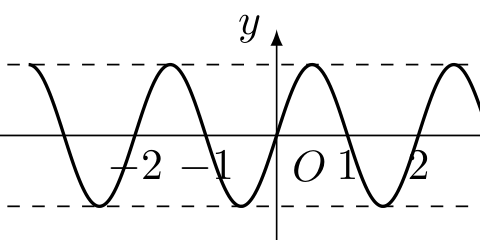
\includegraphics[width=0.15\paperwidth]{GaoKao/images/2011/shaanxi_science/q3_optA_clean.png}  &  \text{B. }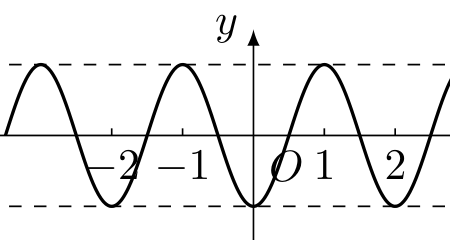
\includegraphics[width=0.15\paperwidth]{GaoKao/images/2011/shaanxi_science/q3_optB_clean.png}  &  \text{C. }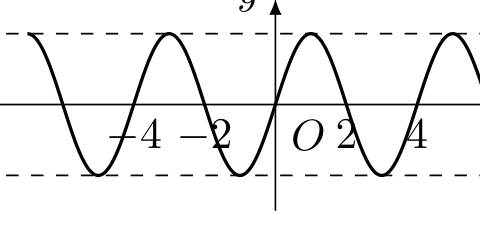
\includegraphics[width=0.15\paperwidth]{GaoKao/images/2011/shaanxi_science/q3_optC_clean.png}  &  \text{D. }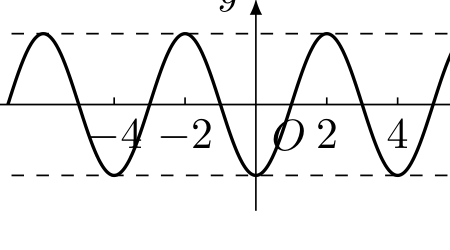
\includegraphics[width=0.15\paperwidth]{GaoKao/images/2011/shaanxi_science/q3_optD_clean.png}
        \end{tabular*}\par}

        \item \((4^{x} - 2^{-x})^{6}\)（\(x \in \mathbb{R}\)）展开式中的常数项是（\quad）

        {\centering\begin{tabular*}{\linewidth}{@{}@{\extracolsep{\fill}}llll@{}}
          \text{A. }\(-20\)  &  \text{B. }\(-15\)  &  \text{C. }15  &  \text{D. }20
        \end{tabular*}\par}

        \item 某几何体的三视图如图所示，则它的体积是（\quad）

\begin{center}
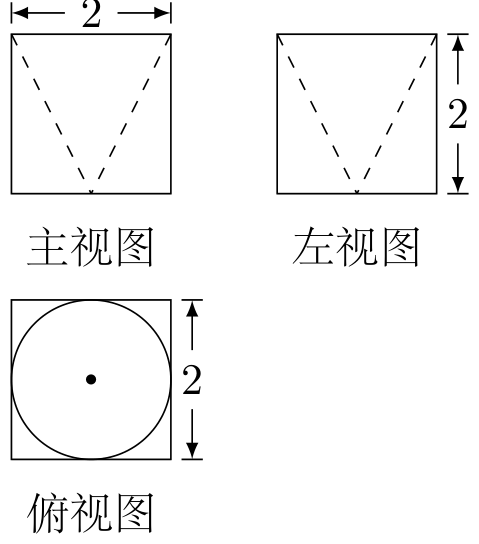
\includegraphics[width=4.7cm]{GaoKao/images/2011/shaanxi_science/q5_fig1.png}
\end{center}

        {\centering\begin{tabular*}{\linewidth}{@{}@{\extracolsep{\fill}}llll@{}}
          \text{A. }\(8 - \frac{2\pi}{3}\)  &  \text{B. }\(8 - \frac{\pi}{3}\)  &  \text{C. }\(8 - 2\pi\)  &  \text{D. }\(\frac{2\pi}{3}\)
        \end{tabular*}\par}

        \item 函数 \( f(x) = \sqrt{x} - \cos x \) 在 \([0, +\infty)\) 内（\quad）

        {\centering\begin{tabular*}{\linewidth}{@{}@{\extracolsep{\fill}}llll@{}}
          \text{A. }没有零点  &  \text{B. }有且仅有一个零点  &  \text{C. }有且仅有两个零点  &  \text{D. }有无穷多个零点
        \end{tabular*}\par}

        \item 设集合 \(M = \{y \mid y = |\cos^2 x - \sin^2 x|, x \in \mathbb{R}\}\)，\(N = \left\{x \mid \left|x - \frac{1}{\i}\right| < \sqrt{2}, x \in \mathbb{R}\right\}\)，其中 \(\i\) 为虚数单位，则 \(M \cap N\) 为（\quad）

        {\centering\begin{tabular*}{\linewidth}{@{}@{\extracolsep{\fill}}llll@{}}
          \text{A. }\((0,1)\)  &  \text{B. }\((0,1]\)  &  \text{C. }\([0,1)\)  &  \text{D. }\([0,1]\)
        \end{tabular*}\par}

        \item 如图，\(x_{1}\)，\(x_{2}\)，\(x_{3}\) 为某次考试三个评阅人对同一道题的独立评分，\(p\) 为该题的最终得分，当 \(x_{1} = 6\)，\(x_{2} = 9\)，\(p = 8.5\) 时，\(x_{3}\) 等于（\quad）

\begin{center}
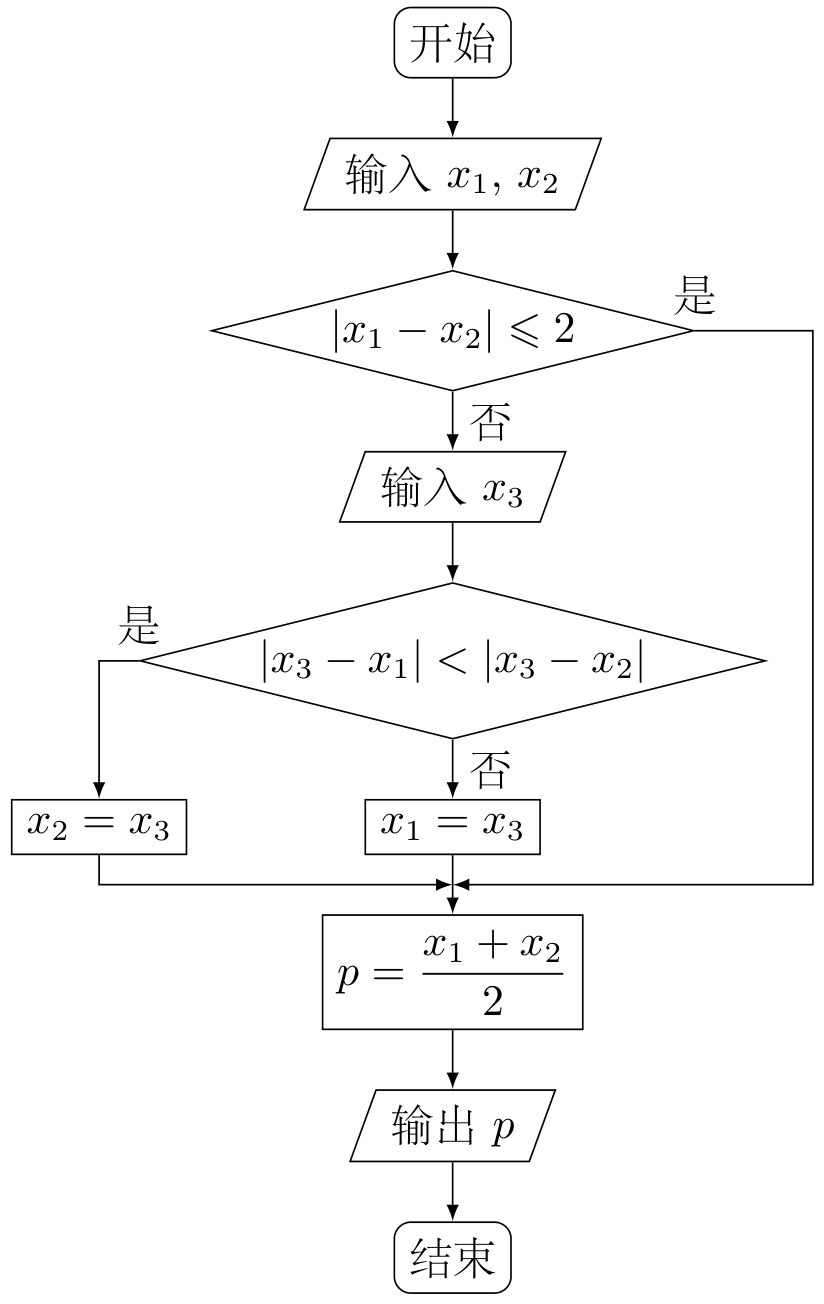
\includegraphics[width=4.7cm]{GaoKao/images/2011/shaanxi_science/q8_fig1.png}
\end{center}

        {\centering\begin{tabular*}{\linewidth}{@{}@{\extracolsep{\fill}}llll@{}}
          \text{A. }11  &  \text{B. }10  &  \text{C. }8  &  \text{D. }7
        \end{tabular*}\par}

        \item 设 \((x_{1}, y_{1})\)，\((x_{2}, y_{2})\)，\(\cdots\)，\((x_{n}, y_{n})\) 是变量 \(x\) 和 \(y\) 的 \(n\) 个样本，直线 \(l\) 是由这些样本点通过最小二乘法得到的线性回归直线（如图），以下结论中正确的是（\quad）

\begin{center}
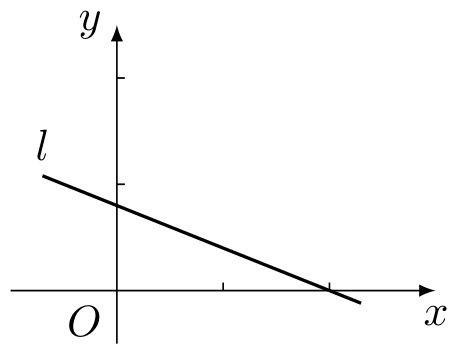
\includegraphics[width=5.3cm]{GaoKao/images/2011/shaanxi_science/q9_fig1.png}
\end{center}

        {\centering\begin{tabular*}{\linewidth}{@{}@{\extracolsep{\fill}}llll@{}}
          \text{A. }\(x\) 和 \(y\) 的相关系数为直线 \(l\) 的斜率  &  \text{B. }\(x\) 和 \(y\) 的相关系数在 \(0\) 到 \(1\) 之间  &  \text{C. }当 \(n\) 为偶数时，分布在 \(l\) 两侧的样本点的个数一定相同  &  \text{D. }直线 \(l\) 过点 \((\bar{x}, \bar{y})\)
        \end{tabular*}\par}

        \item 甲、乙两人一起去游“2011西安世园会”，他们约定：各自独立地从 \(1\) 到 \(6\) 号景点中任选 \(4\) 个进行游览，每个景点参观 \(1\text{ 小时}\)，则最后 \(1\text{ 小时}\) 他们同在一个景点的概率是（\quad）

        {\centering\begin{tabular*}{\linewidth}{@{}@{\extracolsep{\fill}}llll@{}}
          \text{A. }\( \frac{1}{36} \)  &  \text{B. }\( \frac{1}{9} \)  &  \text{C. }\( \frac{5}{36} \)  &  \text{D. }\( \frac{1}{6} \)
        \end{tabular*}\par}

    \end{enumerate}

\end{description}

\begin{description}

    \item[二、填空题]

    \begin{enumerate}[leftmargin=5pt]

      \addtocounter{enumi}{+10}

        \item 设 \(f(x)=\begin{cases}
\lg x, & x>0,\\
x+\int_{0}^{a} 3t^{2}\,dt, & x\leqslant 0
\end{cases}\)，若 \(f(f(1))=1\)，则 \(a=\rule[-0.3ex]{3em}{0.4pt}\).

        \item 设 \(n \in \mathbb{N}^*\)，一元二次方程 \(x^2 - 4x + n = 0\) 有整数根的充要条件是 \(n = \)\rule[-0.3ex]{3em}{0.4pt}.

        \item 观察下列等式 \(1 = 1\)，\(2 + 3 + 4 = 9\)，\(3 + 4 + 5 + 6 + 7 = 25\)，\(4 + 5 + 6 + 7 + 8 + 9 + 10 = 49\). 照此规律，第 \(n\) 个等式应为\rule[-0.3ex]{3em}{0.4pt}.

        \item 植树节某班 \(20\) 名同学在一段直线公路一侧植树，每人植一棵，相邻两棵树相距 \(10\text{ 米}\)，开始时需将树苗集中放置在某一树坑旁边，使每位同学从各自树坑出发前来领取树苗往返所走的路程总和最小，这个最小值为\rule[-0.3ex]{3em}{0.4pt}\(\text{米}\).

    \end{enumerate}

\end{description}

\begin{description}

    \item[三、选做题]

    \begin{enumerate}[leftmargin=5pt]

      \addtocounter{enumi}{+14}

        \item \textbf{【选修4-5：不等式选讲】}

若关于 \(x\) 的不等式 \(\left|a\right| \geqslant \left|x + 1\right| + \left|x - 2\right|\) 存在实数解，则实数 \(a\) 的取值范围是\rule[-0.3ex]{3em}{0.4pt}.

        \item 如图，\(\angle B = \angle D\)，\(AE \perp BC\)，\(\angle ACD = 90^{\circ}\)，且 \(AB = 6\)，\(AC = 4\)，\(AD = 12\)，则 \(BE =\rule[-0.3ex]{3em}{0.4pt}\).

\begin{center}
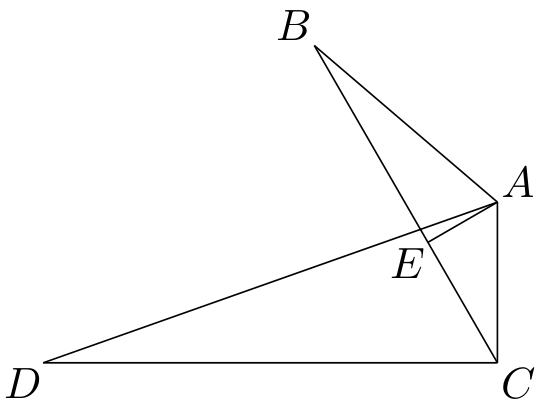
\includegraphics[width=6.8cm]{GaoKao/images/2011/shaanxi_science/q15_fig1.png}
\end{center}

        \item \textbf{【选修4-4：坐标系与参数方程】}

直角坐标系 \(xOy\) 中，以原点为极点，\(x\) 轴正半轴为极轴建立极坐标系，设点 \(A\)，\(B\) 分别在曲线 \( C_{1}:\begin{cases}
x=3+\cos\theta,\\
y=4+\sin\theta,
\end{cases} \)（\(\theta\) 为参数）和曲线 \( C_{2}:\rho=1 \) 上，则 \( |AB| \) 的最小值为\rule[-0.3ex]{3em}{0.4pt}.

    \end{enumerate}

\end{description}

\begin{description}

    \item[四、解答题]

    \begin{enumerate}[leftmargin=5pt]

      \addtocounter{enumi}{+17}

        \item 如图，在 \(\triangle ABC\) 中，\(\angle ABC = 60^{\circ}\)，\(\angle BAC = 90^{\circ}\)，\(AD\) 是 \(BC\) 上的高，沿 \(AD\) 把 \(\triangle ABD\) 折起，使 \(\angle BDC = 90^{\circ}\).
\begin{enumerate}
\item 证明：平面 \(ADB\perp\) 平面 \(BDC\)；
\item 设 \(E\) 为 \(BC\) 的中点，求 \(\overrightarrow{AE}\) 与 \(\overrightarrow{DB}\) 夹角的余弦值.
\end{enumerate}

\begin{center}
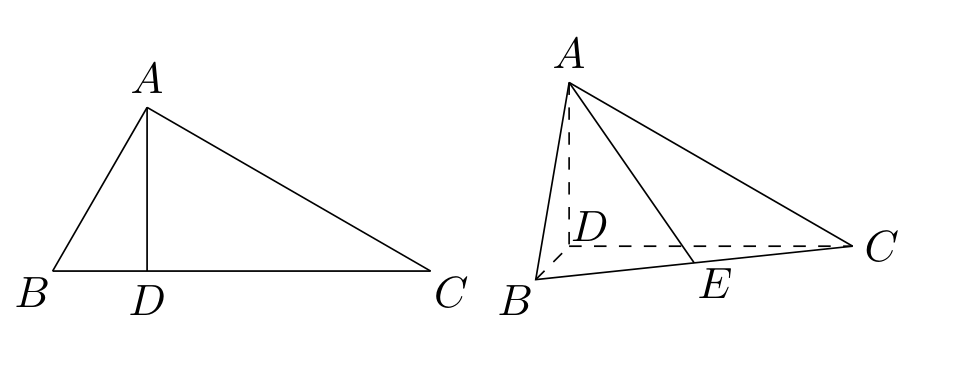
\includegraphics[width=10.5cm]{GaoKao/images/2011/shaanxi_science/q16_fig1.png}
\end{center}

        \item 如图，设 \(P\) 是圆 \(x^{2} + y^{2} = 25\) 上的动点，点 \(D\) 是 \(P\) 在 \(x\) 轴上的投影，\(M\) 为 \(PD\) 上一点，且 \(|MD| = \frac{4}{5} |PD|\).
\begin{enumerate}
\item 当 \(P\) 在圆上运动时，求点 \(M\) 的轨迹 \(C\) 的方程；
\item 求过点 \( (3,0) \) 且斜率为 \( \frac{4}{5} \) 的直线被 \(C\) 所截线段的长度.
\end{enumerate}

\begin{center}
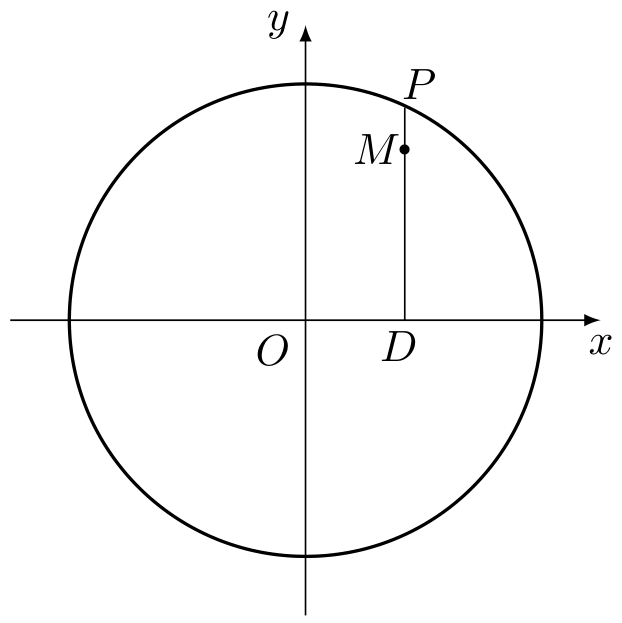
\includegraphics[width=7.7cm]{GaoKao/images/2011/shaanxi_science/q17_fig1.png}
\end{center}

        \item 叙述并证明余弦定理.

        \item 如图，从点 \(P_{1}(0,0)\) 作 \(x\) 轴的垂线交曲线 \(y = {\mathrm{e}}^{x}\) 于点 \(Q_{1}(0,1)\)，曲线在 \(Q_{1}\) 点处的切线与 \(x\) 轴交于点 \(P_{2}\)，再从 \(P_{2}\) 作 \(x\) 轴的垂线交曲线于点 \(Q_{2}\)，依次重复上述过程得到一系列点：\(P_{1}\)，\(Q_{1}\)；\(P_{2}\)，\(Q_{2}\)；\(\cdots\)；\(P_{n}\)，\(Q_{n}\)，记 \(P_{k}\) 点的坐标为 \((x_{k}, 0)\)（\(k = 1, 2, \cdots, n\)）.
\begin{enumerate}
\item 试求 \(x_{k}\) 与 \(x_{k-1}\) 的关系（\(2 \leqslant k \leqslant n\)）；
\item 求 \(\left|P_{1}Q_{1}\right|+\left|P_{2}Q_{2}\right|+\left|P_{3}Q_{3}\right|+\cdots+\left|P_{n}Q_{n}\right|\).
\end{enumerate}

\begin{center}
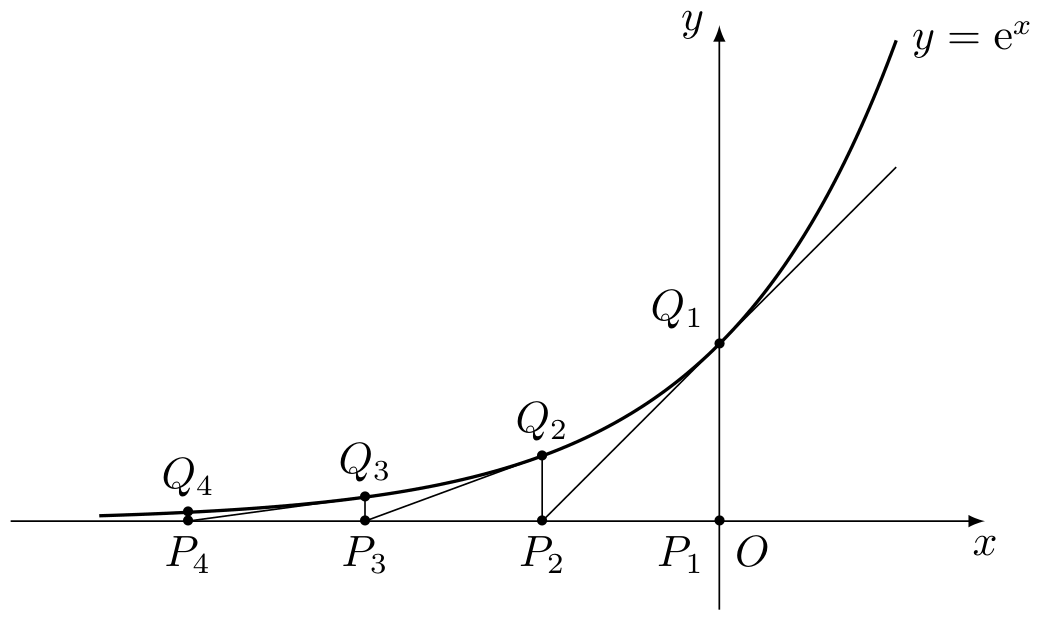
\includegraphics[width=9.9cm]{GaoKao/images/2011/shaanxi_science/q19_fig1.png}
\end{center}

        \item 如图，\(A\) 地到火车站共有两条路径 \(L_{1}\) 和 \(L_{2}\)，据统计，通过两条路径所用的时间互不影响，所用时间落在各时间段内的频率如下表：
\begin{center}
\begin{tabular}{c|ccccc}
\hline
所用时间（分钟） & \(10\sim20\) & \(20\sim30\) & \(30\sim40\) & \(40\sim50\) & \(50\sim60\) \\
\hline
选择 \(L_1\) 的人数 & \(6\) & \(12\) & \(18\) & \(12\) & \(12\) \\
选择 \(L_2\) 的人数 & \(0\) & \(4\) & \(16\) & \(16\) & \(4\) \\
\hline
\end{tabular}
\end{center}
现甲、乙两人分别有 \(40\text{ 分钟}\) 和 \(50\text{ 分钟}\) 时间用于赶往火车站.
\begin{enumerate}
\item 为了尽最大可能在各自允许的时间内赶到火车站，甲和乙应如何选择各自的路径？
\item 用 \(X\) 表示甲、乙两人中在允许的时间内能赶到火车站的人数，针对（1）的选择方案，求 \(X\) 的分布列和数学期望.
\end{enumerate}

\begingroup
\leftskip=0pt\relax
\begin{center}
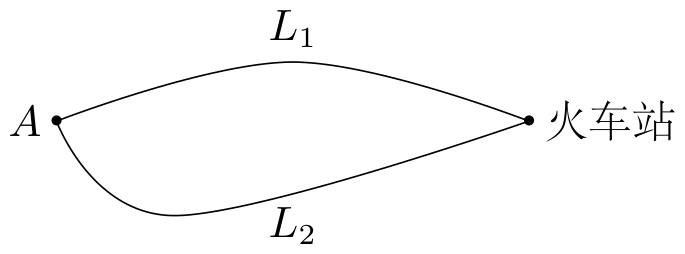
\includegraphics[width=6.9cm]{GaoKao/images/2011/shaanxi_science/q20_fig1.png}
\end{center}
\endgroup

        \item 设函数 \(f(x)\) 定义在 \((0, +\infty)\) 上，\(f(1) = 0\)，导函数 \(f'(x) = \frac{1}{x}\)，\(g(x) = f(x) + f'(x)\).
\begin{enumerate}
\item 求 \(g(x)\) 的单调区间和最小值；
\item 讨论 \(g(x)\) 与 \(g\left(\frac{1}{x}\right)\) 的大小关系；
\item 是否存在 \(x_0 > 0\)，使得 \(|g(x) - g(x_0)| < \frac{1}{2}\) 对任意 \(x > 0\) 成立？若存在，求出 \(x_0\) 的取值范围；若不存在，请说明理由.
\end{enumerate}

    \end{enumerate}

\end{description}


\subsection{2011年陕西卷（文）}\label{gk:2011年陕西卷（文）}

\begin{description}

    \item[一、选择题]

    \begin{enumerate}[leftmargin=5pt]

        \item 设 \(\bm{a}\)，\(\bm{b}\) 是向量，命题“若 \(\bm{a} = -\bm{b}\)，则 \(|\bm{a}| = |\bm{b}|\)”的逆命题是（\quad）

        {\centering\begin{tabular*}{\linewidth}{@{}@{\extracolsep{\fill}}llll@{}}
          \text{A. }若 \(\bm{a} \neq -\bm{b}\)，则 \(|\bm{a}| \neq |\bm{b}|\)  &  \text{B. }若 \(\bm{a} = -\bm{b}\)，则 \(|\bm{a}| \neq |\bm{b}|\)  &  \text{C. }若 \(|\bm{a}| \neq |\bm{b}|\)，则 \(\bm{a} \neq -\bm{b}\)  &  \text{D. }若 \(|\bm{a}| = |\bm{b}|\)，则 \(\bm{a} = -\bm{b}\)
        \end{tabular*}\par}

        \item 设抛物线的顶点在原点，准线方程为 \(x = -2\)，则抛物线的方程是（\quad）

        {\centering\begin{tabular*}{\linewidth}{@{}@{\extracolsep{\fill}}llll@{}}
          \text{A. }\( y^{2} = -8x \)  &  \text{B. }\( y^{2} = -4x \)  &  \text{C. }\( y^{2} = 8x \)  &  \text{D. }\( y^{2} = 4x \)
        \end{tabular*}\par}

        \item 设 \(0 < a < b\)，则下列不等式中正确的是（\quad）

        {\centering\begin{tabular*}{\linewidth}{@{}@{\extracolsep{\fill}}llll@{}}
          \text{A. }\(a < b < \sqrt{ab} < \frac{a + b}{2}\)  &  \text{B. }\(a < \sqrt{ab} < \frac{a + b}{2} < b\)  &  \text{C. }\(a < \sqrt{ab} < b < \frac{a + b}{2}\)  &  \text{D. }\(\sqrt{ab} < a < \frac{a + b}{2} < b\)
        \end{tabular*}\par}

        \item 函数 \( y = x^{\frac{1}{3}} \) 的图象是（\quad）

        {\centering\begin{tabular*}{\linewidth}{@{}@{\extracolsep{\fill}}cccc@{}}
          \text{A. }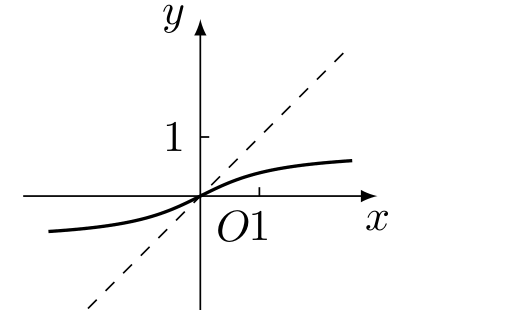
\includegraphics[width=0.15\paperwidth]{GaoKao/images/2011/shaanxi_liberal/q4_optA_clean.png}  &  \text{B. }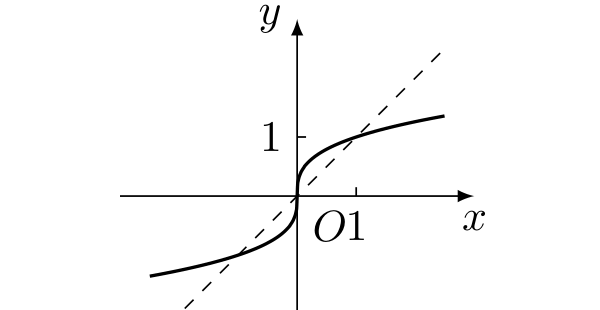
\includegraphics[width=0.15\paperwidth]{GaoKao/images/2011/shaanxi_liberal/q4_optB_clean.png}  &  \text{C. }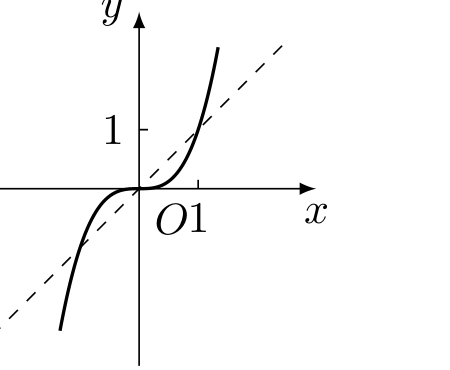
\includegraphics[width=0.15\paperwidth]{GaoKao/images/2011/shaanxi_liberal/q4_optC_clean.png}  &  \text{D. }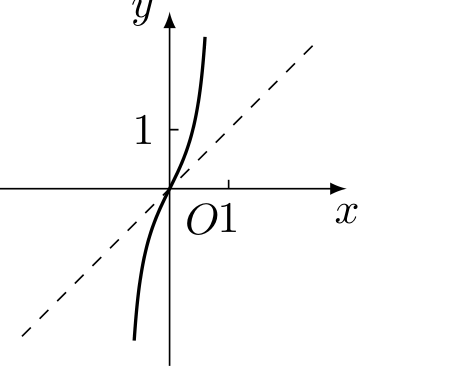
\includegraphics[width=0.15\paperwidth]{GaoKao/images/2011/shaanxi_liberal/q4_optD_clean.png}
        \end{tabular*}\par}

        \item 某几何体的三视图如图所示，则它的体积是（\quad）

\begin{center}
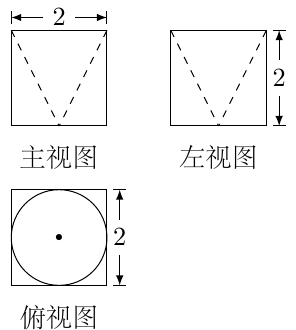
\includegraphics[width=2.4cm]{GaoKao/images/2011/shaanxi_liberal/q5_fig1.png}
\end{center}

        {\centering\begin{tabular*}{\linewidth}{@{}@{\extracolsep{\fill}}llll@{}}
          \text{A. }\(8 - \frac{2\pi}{3}\)  &  \text{B. }\(8 - \frac{\pi}{3}\)  &  \text{C. }\(8 - 2\pi\)  &  \text{D. }\(\frac{2\pi}{3}\)
        \end{tabular*}\par}

        \item 方程 \( |x| = \cos x \) 在 \((- \infty, + \infty)\) 内（\quad）

        {\centering\begin{tabular*}{\linewidth}{@{}@{\extracolsep{\fill}}llll@{}}
          \text{A. }没有根  &  \text{B. }有且仅有一个根  &  \text{C. }有且仅有两个根  &  \text{D. }有无穷多个根
        \end{tabular*}\par}

        \item 下面的框图中，当 \(x_{1} = 6\)，\(x_{2} = 9\)，\(p = 8.5\) 时，\(x_{3}\) 等于（\quad）

\begin{center}
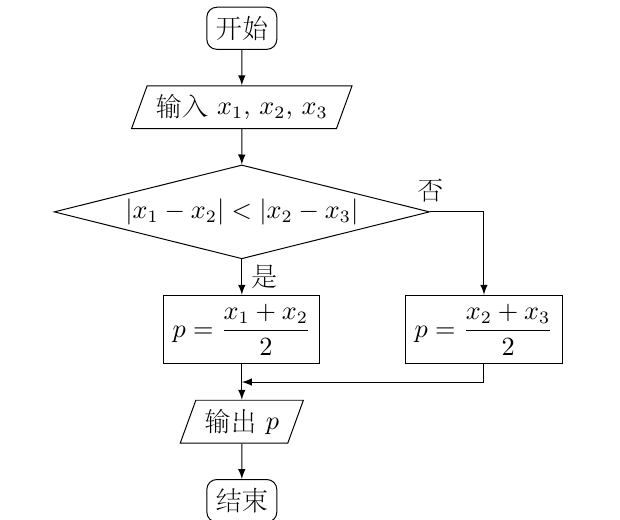
\includegraphics[width=0.52\linewidth]{GaoKao/images/2011/shaanxi_liberal/q7_fig1.png}
\end{center}

        {\centering\begin{tabular*}{\linewidth}{@{}@{\extracolsep{\fill}}llll@{}}
          \text{A. }7  &  \text{B. }8  &  \text{C. }10  &  \text{D. }11
        \end{tabular*}\par}

        \item 设集合 \(M = \{y \mid y = |\cos^2 x - \sin^2 x|, x \in \mathbb{R}\}\)，\(N = \left\{x \mid \left|\frac{x}{\i}\right| < 1,\ \i\text{ 为虚数单位},\ x \in \mathbb{R}\right\}\)，则 \(M \cap N\) 为（\quad）

        {\centering\begin{tabular*}{\linewidth}{@{}@{\extracolsep{\fill}}llll@{}}
          \text{A. }\((0,1)\)  &  \text{B. }\((0,1]\)  &  \text{C. }\([0,1)\)  &  \text{D. }\([0,1]\)
        \end{tabular*}\par}

        \item 设 \((x_{1}, y_{1})\)，\((x_{2}, y_{2})\)，\(\cdots\)，\((x_{n}, y_{n})\) 是变量 \(x\) 和 \(y\) 的 \(n\) 个样本点，直线 \(l\) 是由这些样本点通过最小二乘法得到的线性回归直线（如图），以下结论中正确的是（\quad）

\begin{center}
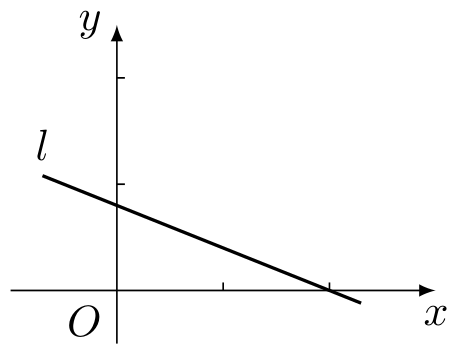
\includegraphics[width=5.3cm]{GaoKao/images/2011/shaanxi_liberal/q9_fig1.png}
\end{center}

        {\centering\begin{tabular*}{\linewidth}{@{}@{\extracolsep{\fill}}llll@{}}
          \text{A. }直线 \(l\) 过点 \((\overline{x}, \overline{y})\)  &  \text{B. }\(x\) 和 \(y\) 的相关系数为直线 \(l\) 的斜率  &  \text{C. }\(x\) 和 \(y\) 的相关系数在 \(0\) 到 \(1\) 之间  &  \text{D. }当 \(n\) 为偶数时，分布在 \(l\) 两侧的样本点的个数一定相同
        \end{tabular*}\par}

        \item 植树节某班 \(20\) 名同学在一段直线公路一侧植树，每人植一棵，相邻两棵树相距 \(10\text{ 米}\)，开始时需将树苗集中放置在某一树坑旁边，现将树坑从 \(1\) 到 \(20\) 依次编号，为使各位同学从各自树坑前来领取树苗所走的路程总和最小，树苗可以放置的两个最佳坑位的编号为（\quad）

        {\centering\begin{tabular*}{\linewidth}{@{}@{\extracolsep{\fill}}llll@{}}
          \text{A. }\(1\) 和 \(20\)  &  \text{B. }\(9\) 和 \(10\)  &  \text{C. }\(9\) 和 \(11\)  &  \text{D. }\(10\) 和 \(11\)
        \end{tabular*}\par}

    \end{enumerate}

\end{description}

\begin{description}

    \item[二、填空题]

    \begin{enumerate}[leftmargin=5pt]

      \addtocounter{enumi}{+10}

        \item 设函数 \( f(x) = \begin{cases}
\lg x, & x > 0,\\
10^x, & x \leqslant 0.
\end{cases} \) 则 \( f(f(-2)) = \)\rule[-0.3ex]{3em}{0.4pt}.

        \item 如图，点 \((x, y)\) 在四边形 \(ABCD\) 内部和边界上运动，那么 \(2x - y\) 的最小值为\rule[-0.3ex]{3em}{0.4pt}.

\begin{center}
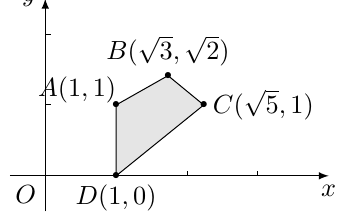
\includegraphics[width=4.4cm]{GaoKao/images/2011/shaanxi_liberal/q12_fig1.png}
\end{center}

        \item 观察下列等式 \(1 = 1\)，\(2 + 3 + 4 = 9\)，\(3 + 4 + 5 + 6 + 7 = 25\)，\(4 + 5 + 6 + 7 + 8 + 9 + 10 = 49\)，\(\dots\). 照此规律，第五个等式应为\rule[-0.3ex]{3em}{0.4pt}.

        \item 设 \(n \in \mathbb{N}_{+}\)，一元二次方程 \(x^{2} - 4x + n = 0\) 有整数根的充要条件是 \(n=\)\rule[-0.3ex]{3em}{0.4pt}.

    \end{enumerate}

\end{description}

\begin{description}

    \item[三、选做题]

    \begin{enumerate}[leftmargin=5pt]

      \addtocounter{enumi}{+14}

        \item \textbf{【选修4-5：不等式选讲】}

若不等式 \( |x+1|+|x-2|\geqslant a \) 对任意 \( x\in\mathbb{R} \) 恒成立，则 \(a\) 的取值范围是\rule[-0.3ex]{3em}{0.4pt}.

        \item 如图，\( \angle B = \angle D\)，\( AE \perp BC\)，\( \angle ACD = 90^{\circ}\)，且 \(AB = 6\)，\(AC = 4\)，\(AD = 12\)，则 \(AE =\)\rule[-0.3ex]{3em}{0.4pt}.

\begin{center}
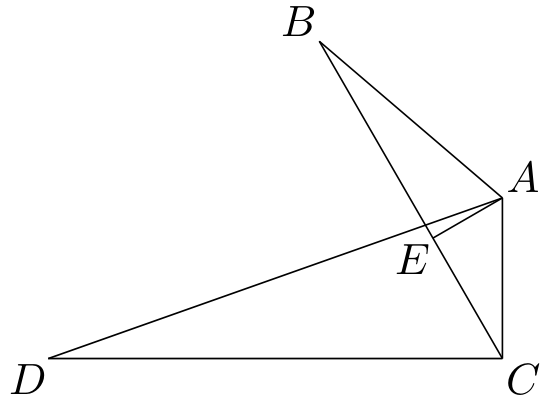
\includegraphics[width=6.8cm]{GaoKao/images/2011/shaanxi_liberal/q15_fig1.png}
\end{center}

        \item \textbf{【选修4-4：坐标系与参数方程】}

直角坐标系 \(xOy\) 中，以原点为极点，\(x\) 轴正半轴为极轴建立极坐标系，设点 \(A\)，\(B\) 分别在曲线 \(C_1: \begin{cases}
x = 3 + \cos \theta,\\
y = \sin \theta,
\end{cases}\) （\(\theta\) 为参数）和曲线 \(C_2: \rho = 1\) 上，则 \(|AB|\) 的最小值为\rule[-0.3ex]{3em}{0.4pt}.

    \end{enumerate}

\end{description}

\begin{description}

    \item[四、解答题]

    \begin{enumerate}[leftmargin=5pt]

      \addtocounter{enumi}{+17}

        \item 如图，在 \(\triangle ABC\) 中，\(\angle ABC = 45^{\circ}\)，\(\angle BAC = 90^{\circ}\)，\(AD\) 是 \(BC\) 上的高，沿 \(AD\) 把 \(\triangle ABD\) 折起，使 \(\angle BDC = 90^{\circ}\).

\begin{enumerate}
\item 证明：平面 \(ADB \perp\) 平面 \(BDC\)；
\item 若 \(BD = 1\)，求三棱锥 \(D - ABC\) 的表面积.
\end{enumerate}

\begin{center}
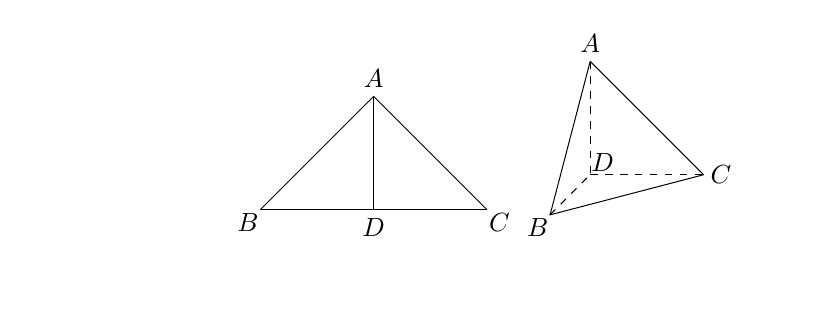
\includegraphics[width=10.5cm]{GaoKao/images/2011/shaanxi_liberal/q16_fig1.png}
\end{center}

        \item 设椭圆 \(C: \frac{x^2}{a^2} + \frac{y^2}{b^2} = 1\)（\(a > b > 0\)）过点 \((0,4)\)，离心率为 \(\frac{3}{5}\).

\begin{enumerate}
\item 求 \(C\) 的方程；
\item 求过点 \((3,0)\) 且斜率为 \(\frac{4}{5}\) 的直线被 \(C\) 所截线段的中点坐标.
\end{enumerate}

        \item 叙述并证明余弦定理.

        \item 如图，从点 \(P_{1}(0,0)\) 作 \(x\) 轴的垂线交曲线 \(y = {\mathrm{e}}^{x}\) 于点 \(Q_{1}(0,1)\)，曲线在 \(Q_{1}\) 点处的切线与 \(x\) 轴交于点 \(P_{2}\)，再从 \(P_{2}\) 作 \(x\) 轴的垂线交曲线于点 \(Q_{2}\)，依次重复上述过程得到一系列点：\(P_{1}\)，\(Q_{1}\)；\(P_{2}\)，\(Q_{2}\)；\(\cdots\)；\(P_{n}\)，\(Q_{n}\)，记 \(P_{k}\) 点的坐标为 \((x_{k}, 0)\)（\(k = 1\)，\(2\)，\(\cdots\)，\(n\)）.

\begin{enumerate}
\item 试求 \(x_{k}\) 与 \(x_{k-1}\) 的关系（\(2 \leqslant k \leqslant n\)）；
\item 求 \( \left|P_{1}Q_{1}\right|+\left|P_{2}Q_{2}\right|+\left|P_{3}Q_{3}\right|+\cdots+\left|P_{n}Q_{n}\right| \).
\end{enumerate}

\begin{center}
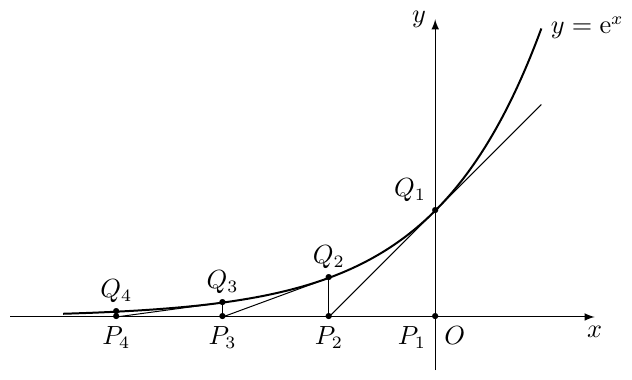
\includegraphics[width=10.3cm]{GaoKao/images/2011/shaanxi_liberal/q19_fig1.png}
\end{center}

        \item 如图，\(A\) 地到火车站共有两条路径 \(L_{1}\) 和 \(L_{2}\)，现随机抽取 \(100\) 位从 \(A\) 地到达火车站的人进行调查，调查结果如下：

\begin{center}
\begin{tabular}{c|ccccc}
\hline
所用时间（分钟） & \(10\sim20\) & \(20\sim30\) & \(30\sim40\) & \(40\sim50\) & \(50\sim60\) \\
\hline
选择 \(L_{1}\) 的人数 & \(6\) & \(12\) & \(18\) & \(12\) & \(12\) \\
选择 \(L_{2}\) 的人数 & \(0\) & \(4\) & \(16\) & \(16\) & \(4\) \\
\hline
\end{tabular}
\end{center}

\begin{enumerate}
\item 试估计 \(40\text{ 分钟}\) 内不能赶到火车站的概率；
\item 分别求通过路径 \(L_{1}\) 和 \(L_{2}\) 所用时间落在上表中各时间段内的频率；
\item 现甲，乙两人分别有 \(40\text{ 分钟}\) 和 \(50\text{ 分钟}\) 时间用于赶往火车站，为了尽最大可能在允许的时间内赶到火车站，试通过计算说明，他们应如何选择各自的路径.
\end{enumerate}

\begin{center}
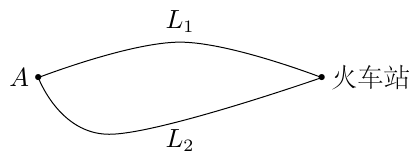
\includegraphics[width=7.4cm]{GaoKao/images/2011/shaanxi_liberal/q20_fig1.png}
\end{center}

        \item 设 \(f(x) = \ln x\)，\(g(x) = f(x) + f'(x)\).

\begin{enumerate}
\item 求 \(g(x)\) 的单调区间和最小值；
\item 讨论 \(g(x)\) 与 \(g\left(\frac{1}{x}\right)\) 的大小关系；
\item 求 \(a\) 的取值范围，使得 \(g(a) - g(x) < \frac{1}{a}\) 对任意 \(x > 0\) 成立.
\end{enumerate}

    \end{enumerate}

\end{description}


\subsection{2011年天津卷（理）}\label{gk:2011年天津卷（理）}

\begin{description}

    \item[一、选择题]

    \begin{enumerate}[leftmargin=5pt]

        \item \(i\) 是虚数单位，复数 \( \frac{1-3\i}{1-\i}= \)（\quad）

        {\centering\begin{tabular*}{\linewidth}{@{}@{\extracolsep{\fill}}llll@{}}
          \text{A. }\(2 + \i\)  &  \text{B. }\(2 - \i\)  &  \text{C. }\(-1 + 2\i\)  &  \text{D. }\(-1 - 2\i\)
        \end{tabular*}\par}

        \item 设 \(x\)，\(y \in \mathbb{R}\)，则“\(x \geqslant 2\) 且 \(y \geqslant 2\)”是“\(x^2 + y^2 \geqslant 4\)”的（\quad）

        {\centering\begin{tabular*}{\linewidth}{@{}@{\extracolsep{\fill}}llll@{}}
          \text{A. }充分而不必要条件  &  \text{B. }必要而不充分条件  &  \text{C. }充分必要条件  &  \text{D. }既不充分也不必要条件
        \end{tabular*}\par}

        \item 阅读下面的程序框图，运行相应的程序，则输出 \(i\) 的值为（\quad）

\begin{center}
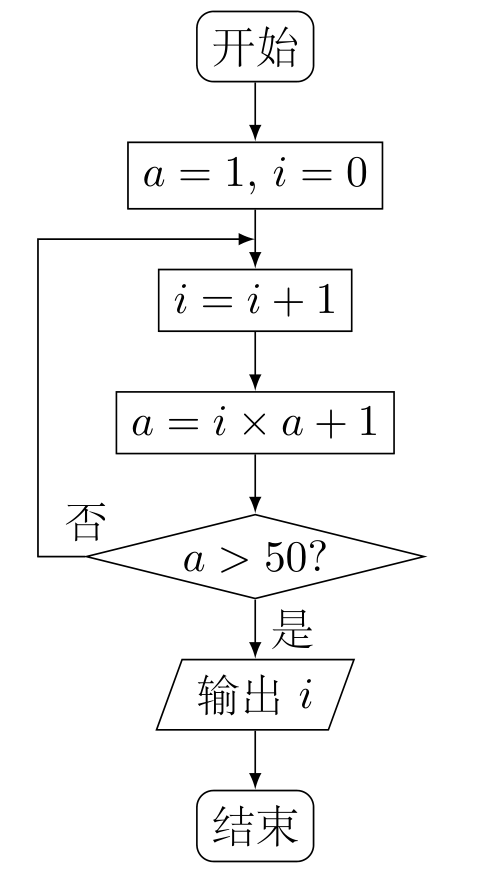
\includegraphics[width=0.70\linewidth]{GaoKao/images/2011/tianjin_science/q3_fig1.png}
\end{center}

        {\centering\begin{tabular*}{\linewidth}{@{}@{\extracolsep{\fill}}llll@{}}
          \text{A. }3  &  \text{B. }4  &  \text{C. }5  &  \text{D. }6
        \end{tabular*}\par}

        \item 已知 \( \{a_{n}\} \) 为等差数列，其公差为 \(-2\)，且 \( a_{7} \) 是 \( a_{3} \) 与 \( a_{9} \) 的等比中项，\( S_{n} \) 为 \( \{a_{n}\} \) 的前 \(n\) 项和，\( n \in \mathbb{N}^{*} \)，则 \(S_{10}\) 的值为（\quad）

        {\centering\begin{tabular*}{\linewidth}{@{}@{\extracolsep{\fill}}llll@{}}
          \text{A. }\(-110\)  &  \text{B. }\(-90\)  &  \text{C. }90  &  \text{D. }110
        \end{tabular*}\par}

        \item 在 \(\left(\frac{\sqrt{x}}{2} - \frac{2}{\sqrt{x}}\right)^{6}\) 的二项展开式中，\(x^{2}\) 的系数为（\quad）

        {\centering\begin{tabular*}{\linewidth}{@{}@{\extracolsep{\fill}}llll@{}}
          \text{A. }\(-\frac{15}{4}\)  &  \text{B. }\( \frac{15}{4} \)  &  \text{C. }\(-\frac{3}{8}\)  &  \text{D. }\(\frac{3}{8}\)
        \end{tabular*}\par}

        \item 如图所示，在 \(\triangle ABC\) 中，\(D\) 是边 \(AC\) 上的点，且 \(AB = AD\)，\(2AB = \sqrt{3}BD\)，\(BC = 2BD\)，则 \(\sin C\) 的值为（\quad）

\begin{center}
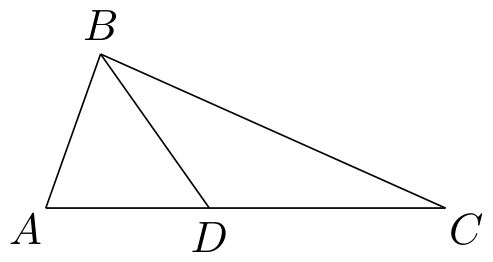
\includegraphics[width=6.1cm]{GaoKao/images/2011/tianjin_science/q6_fig1.png}
\end{center}

        {\centering\begin{tabular*}{\linewidth}{@{}@{\extracolsep{\fill}}llll@{}}
          \text{A. }\(\frac{\sqrt{3}}{3}\)  &  \text{B. }\(\frac{\sqrt{3}}{6}\)  &  \text{C. }\(\frac{\sqrt{6}}{3}\)  &  \text{D. }\(\frac{\sqrt{6}}{6}\)
        \end{tabular*}\par}

        \item 已知 \(a = 5^{\log_{2} 3^{4}}\)，\(b = 5^{\log_{4} 3^{6}}\)，\(c = \left(\frac{1}{5}\right)^{\log_{3} 0.3}\)，则（\quad）

        {\centering\begin{tabular*}{\linewidth}{@{}@{\extracolsep{\fill}}llll@{}}
          \text{A. }\(a > b > c\)  &  \text{B. }\(b > a > c\)  &  \text{C. }\(a > c > b\)  &  \text{D. }\(c > a > b\)
        \end{tabular*}\par}

        \item 对实数 \(a\) 与 \(b\)，定义运算“\(\otimes\)”： \(a \otimes b = \begin{cases}
a, & a - b \leqslant 1,\\
b, & a - b > 1.
\end{cases}\) 设函数 \(f(x) = (x^2 - 2) \otimes (x - x^2)\)，\(x \in \mathbb{R}\). 若函数 \(y = f(x) - c\) 的图象与 \(x\) 轴恰有两个公共点，则实数 \(c\) 的取值范围是（\quad）

        {\centering\begin{tabular*}{\linewidth}{@{}@{\extracolsep{\fill}}llll@{}}
          \text{A. }\((- \infty, -2] \cup \left(-1, \frac{3}{2}\right)\)  &  \text{B. }\((-\infty, -2] \cup \left(-1, -\frac{3}{4}\right)\)  &  \text{C. }\(\left(-1, \frac{1}{4}\right) \cup \left(\frac{1}{4}, +\infty\right)\)  &  \text{D. }\(\left(-1, -\frac{3}{4}\right) \cup \left[\frac{1}{4}, +\infty\right)\)
        \end{tabular*}\par}

    \end{enumerate}

\end{description}

\begin{description}

    \item[二、填空题]

    \begin{enumerate}[leftmargin=5pt]

      \addtocounter{enumi}{+8}

        \item 一支田径队有男运动员 48 人，女运动员 36 人，若用分层抽样的方法从该队的全体运动员中抽取一个容量为 21 的样本，则抽取男运动员的人数为\rule[-0.3ex]{3em}{0.4pt}.

        \item 一个几何体的三视图如图所示（单位：m），则这个几何体的体积为\rule[-0.3ex]{3em}{0.4pt} \(\text{m}^{3}\).

\begin{center}
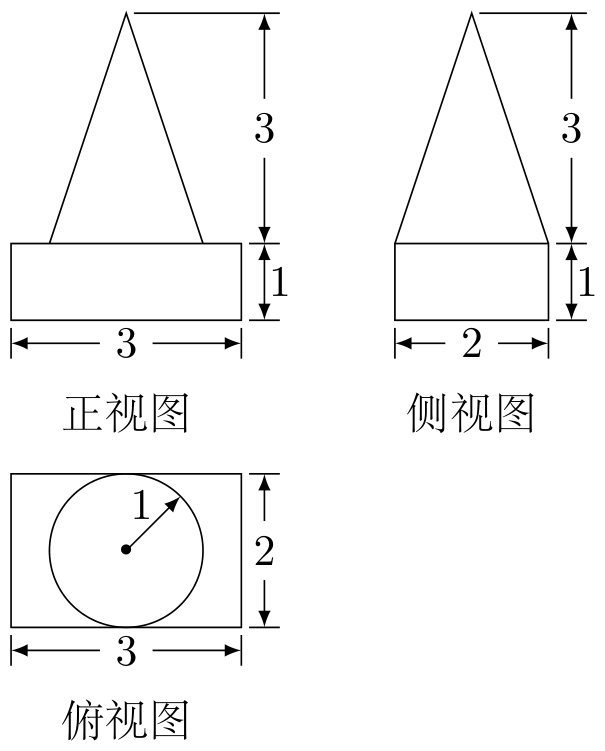
\includegraphics[width=5.9cm]{GaoKao/images/2011/tianjin_science/q10_fig1.png}
\end{center}

        \item 已知抛物线 \(C\) 的参数方程为
\(\begin{cases}
x = 8t^{2},\\
y = 8t,
\end{cases}\)
（\(t\) 为参数），若斜率为 1 的直线经过抛物线 \(C\) 的焦点，且与圆 \( (x - 4)^{2} + y^{2} = r^{2} \) （\(r > 0\)）相切，则 \(r =\)\rule[-0.3ex]{3em}{0.4pt}.

        \item 如图，已知圆中两条弦 \(AB\) 与 \(CD\) 相交于点 \(F\)，\(E\) 是 \(AB\) 延长线上一点，且 \(DF = CF = \sqrt{2}\)，\(AF:FB:BE = 4:2:1\).
若 \(CE\) 与圆相切，则 \(CE\) 的长为\rule[-0.3ex]{3em}{0.4pt}.

\begin{center}
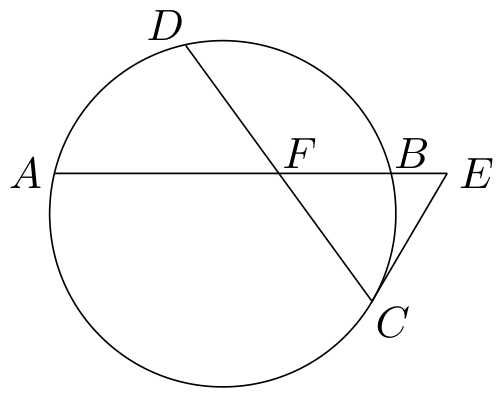
\includegraphics[width=6.2cm]{GaoKao/images/2011/tianjin_science/q12_fig1.png}
\end{center}

        \item 已知集合 \(A = \{x \in \mathbb{R} \mid |x + 3| + |x - 4| \leqslant 9\}\)，\(B = \left\{x \in \mathbb{R} \mid x = 4t + \frac{1}{t} - 6, t \in (0, +\infty)\right\}\)，则集合 \(A \cap B = \)\rule[-0.3ex]{3em}{0.4pt}.

        \item 已知直角梯形 \(ABCD\) 中，\(AD \parallel BC\)，\(\angle ADC = 90^{\circ}\)，\(AD = 2\)，\(BC = 1\)，\(P\) 是腰 \(DC\) 上的动点，则 \(\left|\overrightarrow{PA} + 3\overrightarrow{PB}\right|\) 的最小值为\rule[-0.3ex]{3em}{0.4pt}.

    \end{enumerate}

\end{description}

\begin{description}

    \item[三、解答题]

    \begin{enumerate}[leftmargin=5pt]

      \addtocounter{enumi}{+14}

        \item 已知函数 \( f(x) = \tan \left(2x + \frac{\pi}{4}\right) \).
\begin{enumerate}
\item 求 \( f(x) \) 的定义域与最小正周期；
\item 设 \(\alpha \in (0, \frac{\pi}{4})\)，若 \(f\left(\frac{\alpha}{2}\right) = 2\cos 2\alpha\)，求 \(\alpha\) 的大小.
\end{enumerate}

        \item 学校游园活动有这样一个游戏项目：甲箱子里装有3个白球，2个黑球，乙箱子里装有1个白球，2个黑球，这些球除颜色外完全相同. 每次游戏从这两个箱子里各随机摸出2个球，若摸出的白球不少于2个，则获奖. （每次游戏结束后将球放回原箱）
\begin{enumerate}
\item 求在一次游戏中
\begin{enumerate}
    \item 摸出 3 个白球的概率；
    \item 获奖的概率.
\end{enumerate}
\item 求在两次中获奖次数 X 的分布列及数学期望 \( E(X) \).
\end{enumerate}

        \item 如图，在三棱柱 \(ABC - A_{1}B_{1}C_{1}\) 中，\(H\) 是正方形 \(AA_{1}B_{1}B\) 的中心，\(AA_{1} = 2\sqrt{2}\)，\(C_{1}H \perp\) 平面 \(AA_{1}B_{1}B\)，且 \(C_{1}H = \sqrt{5}\).
\begin{enumerate}
\item 求异面直线 \(AC\) 与 \(A_{1}B_{1}\) 所成角的余弦值；
\item 求二面角 \(A - A_{1}C_{1} - B_{1}\) 的正弦值；
\item 设 \(N\) 为棱 \(B_{1}C_{1}\) 的中点，点 \(M\) 在平面 \(AA_{1}B_{1}B\) 内，且 \(MN \perp\) 平面 \(A_{1}B_{1}C_{1}\)，求线段 \(BM\) 的长.
\end{enumerate}
\begin{center}
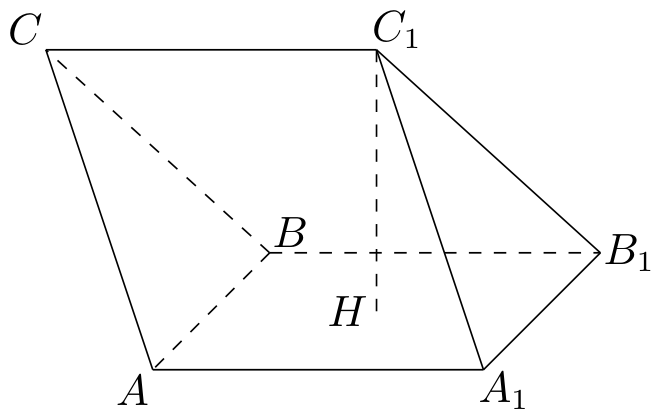
\includegraphics[width=6.5cm]{GaoKao/images/2011/tianjin_science/q17_fig1.png}
\end{center}

        \item 已知 \(a > 0\)，函数 \(f(x) = \ln x - ax^2\)，\(x > 0\).（\(f(x)\) 的图象连续不断）
\begin{enumerate}
\item 求 \( f(x) \) 的单调区间；
\item 当 \(a = \frac{1}{8}\) 时，证明：存在 \(x_0 \in (2, +\infty)\)，使 \(f(x_0) = f\left(\frac{3}{2}\right)\).
\item 若存在均属于区间 \([1,3]\) 的 \(\alpha\)，\(\beta\)，且 \(\beta - \alpha \geqslant 1\)，使 \(f(\alpha) = f(\beta)\). 证明： \(\frac{\ln 3 - \ln 2}{5} \leqslant a \leqslant \frac{\ln 2}{3}\).
\end{enumerate}

        \item 已知数列 \(\{a_{n}\}\) 与 \(\{b_{n}\}\) 满足： \(b_{n}a_{n} + a_{n + 1} + b_{n + 1}a_{n + 2} = 0\)，\(b_{n} = \frac{3 + (-1)^{n}}{2}\)，\(n \in \mathbb{N}^{*}\)，且 \(a_{1} = 2\)，\(a_{2} = 4\)，
\begin{enumerate}
\item 求 \(a_{3}\)，\(a_{4}\)，\(a_{5}\) 的值；
\item 设 \(c_{n} = a_{2n - 1} + a_{2n + 1}\)，\(n \in \mathbb{N}^{*}\)，证明： \(\{c_{n}\}\) 是等比数列；
\item 设 \(S_{k} = a_{2} + a_{4} + \dots + a_{2k}\)，\(k \in \mathbb{N}^{*}\)，证明： \(\sum_{k=1}^{n} \frac{S_{k}}{a_{k}} < \frac{7}{6}\)（\(n \in \mathbb{N}^{*}\)）.
\end{enumerate}

        \item 在平面直角坐标系 \(xOy\) 中，点 \(P(a,b)\) （\(a > b > 0\)） 为动点，\(F_{1}\)，\(F_{2}\) 分别为椭圆 \(\frac{x^2}{a^2} + \frac{y^2}{b^2} = 1\) 的左，右焦点. 已知 \(\triangle F_1PF_2\) 为等腰三角形.
\begin{enumerate}
\item 求椭圆的离心率 \(e\)；
\item 设直线 \(PF_{2}\) 与椭圆相交于 \(A\)，\(B\) 两点，\(M\) 是直线 \(PF_{2}\) 上的点，满足 \(\overrightarrow{AM} \cdot \overrightarrow{BM} = -2\)，求点 \(M\) 的轨迹方程.
\end{enumerate}

    \end{enumerate}

\end{description}


\subsection{2011年天津卷（文）}\label{gk:2011年天津卷（文）}

\begin{description}

    \item[一、选择题]

    \begin{enumerate}[leftmargin=5pt]

        \item \(\i\) 是虚数单位，复数 \(\frac{1 - 3\i}{1 - \i} =\)（\quad）

        {\centering\begin{tabular*}{\linewidth}{@{}@{\extracolsep{\fill}}llll@{}}
          \text{A. }\(2 - \i\)  &  \text{B. }\(2 + \i\)  &  \text{C. }\(-1 - 2\i\)  &  \text{D. }\(-1 + 2\i\)
        \end{tabular*}\par}

        \item 设变量 \(x\)，\(y\) 满足的约束条件 \(\begin{cases}
x\geqslant 1,\\
x+y-4\leqslant 0,\\
x-3y+4\leqslant 0
\end{cases}\)，则目标函数 \(z = 3x - y\) 的最大值为（\quad）

        {\centering\begin{tabular*}{\linewidth}{@{}@{\extracolsep{\fill}}llll@{}}
          \text{A. }\(-4\)  &  \text{B. }\(0\)  &  \text{C. }\( \frac{4}{3} \)  &  \text{D. }\(4\)
        \end{tabular*}\par}

        \item 阅读程序框图，运行相应的程序，若输入 \(x\) 的值为 \(-4\)，则输出 \(y\) 的值为（\quad）

\begin{center}
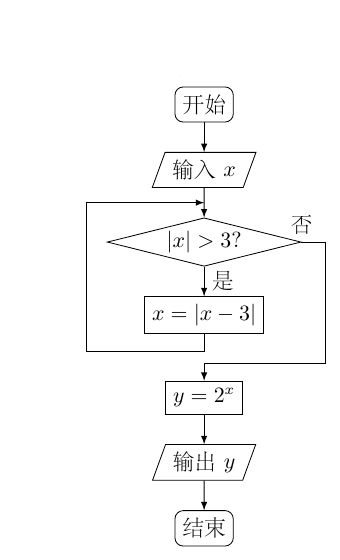
\includegraphics[width=0.70\linewidth]{GaoKao/images/2011/tianjin_liberal/q3_fig1.png}
\end{center}

        {\centering\begin{tabular*}{\linewidth}{@{}@{\extracolsep{\fill}}llll@{}}
          \text{A. }\(0.5\)  &  \text{B. }\(1\)  &  \text{C. }\(2\)  &  \text{D. }\(4\)
        \end{tabular*}\par}

        \item 设集合 \(A = \{x \in \mathbb{R} \mid x - 2 > 0\}\)，\(B = \{x \in \mathbb{R} \mid x < 0\}\)，\(C = \{x \in \mathbb{R} \mid x(x - 2) > 0\}\)，则“\(x \in A \cup B\)”是“\(x \in C\)”的（\quad）

        {\centering\begin{tabular*}{\linewidth}{@{}@{\extracolsep{\fill}}llll@{}}
          \text{A. }充分而不必要条件  &  \text{B. }必要而不充分条件  &  \text{C. }充分必要条件  &  \text{D. }既不充分也不必要条件
        \end{tabular*}\par}

        \item 已知 \(a = \log_2 3.6\)，\(b = \log_4 3.2\)，\(c = \log_4 3.6\) 则（\quad）

        {\centering\begin{tabular*}{\linewidth}{@{}@{\extracolsep{\fill}}llll@{}}
          \text{A. }\(a > b > c\)  &  \text{B. }\(a > c > b\)  &  \text{C. }\(b > a > c\)  &  \text{D. }\(c > a > b\)
        \end{tabular*}\par}

        \item 已知双曲线 \(\frac{x^2}{a^{2}} - \frac{y^2}{b^{2}} = 1 \) （\(a > 0, b > 0\)）的左顶点与抛物线 \(y^2 = 2px\) （\(p > 0\)） 的焦点的距离为4，且双曲线的一条渐近线与抛物线的准线的交点坐标为 \((-2, -1)\)，则双曲线的焦距为（\quad）

        {\centering\begin{tabular*}{\linewidth}{@{}@{\extracolsep{\fill}}llll@{}}
          \text{A. }\(2\sqrt{3}\)  &  \text{B. }\(2\sqrt{5}\)  &  \text{C. }\(4\sqrt{3}\)  &  \text{D. }\(4\sqrt{5}\)
        \end{tabular*}\par}

        \item 已知函数 \(f(x) = 2\sin (\omega x + \varphi)\)，\(x \in \mathbb{R}\)，其中 \(\omega > 0\)，\(-\pi < \varphi \leqslant \pi\). 若 \( f(x) \) 的最小正周期为 \( 6\pi \)，且当 \( x = \frac{\pi}{2} \) 时，\( f(x) \) 取得最大值，则（\quad）

        {\centering\begin{tabular*}{\linewidth}{@{}@{\extracolsep{\fill}}llll@{}}
          \text{A. }\(f(x)\) 在区间 \([-2\pi, 0]\) 上是增函数  &  \text{B. }\(f(x)\) 在区间 \([-3\pi, -\pi]\) 上是增函数  &  \text{C. }\(f(x)\) 在区间 \([3\pi, 5\pi]\) 上是减函数  &  \text{D. }\(f(x)\) 在区间 \([4\pi, 6\pi]\) 上是减函数
        \end{tabular*}\par}

        \item 对实数 \(a\) 和 \(b\)，定义运算“\(\otimes\)”： \( a \otimes b = \begin{cases}
a, & a - b \leqslant 1,\\
b, & a - b > 1.
\end{cases} \) 设函数 \(f(x) = (x^{2} - 2) \otimes (x - 1)\)，\(x \in \mathbb{R}\). 若函数 \( y = f(x) - c \) 的图象与 \(x\) 轴恰有两个公共点，则实数 \(c\) 的取值范围是（\quad）

        {\centering\begin{tabular*}{\linewidth}{@{}@{\extracolsep{\fill}}llll@{}}
          \text{A. }\((-1,1]\cup (2, + \infty)\)  &  \text{B. }\((-2, - 1] \cup (1, 2]\)  &  \text{C. }\((-\infty, -2) \cup (1, 2]\)  &  \text{D. }\([-2, - 1]\)
        \end{tabular*}\par}

    \end{enumerate}

\end{description}

\begin{description}

    \item[二、填空题]

    \begin{enumerate}[leftmargin=5pt]

      \addtocounter{enumi}{+8}

        \item 已知集合 \(A = \{x \in \mathbb{R} \mid |x - 1| < 2\}\)，\(\mathbb{Z}\) 为整数集，则集合 \(A \cap \mathbb{Z}\) 中所有元素的和等于\rule[-0.3ex]{3em}{0.4pt}.

        \item 一个几何体的三视图如图所示（单位：m），则这个几何体的体积为\rule[-0.3ex]{3em}{0.4pt}\(\mathrm{m}^{3}\).

\begin{center}
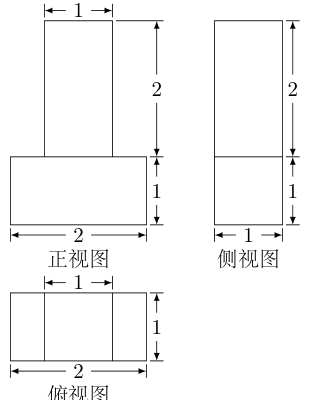
\includegraphics[width=5.5cm]{GaoKao/images/2011/tianjin_liberal/q10_fig1.png}
\end{center}

        \item 已知 \( \{a_{n}\} \) 为等差数列，\( S_{n} \) 为其前 \(n\) 项和. \( n \in \mathbb{N}^{*} \). 若 \( a_{3} = 16 \)，\( S_{20} = 20 \)，则 \(S_{10}\) 的值为\rule[-0.3ex]{3em}{0.4pt}.

        \item 已知 \(\log_2 a + \log_2 b \geqslant 1\)，则 \(3^a + 9^b\) 的最小值为\rule[-0.3ex]{3em}{0.4pt}.

        \item 如图，已知圆中两条弦 \(AB\) 与 \(CD\) 相交于点 \(F\)，\(E\) 是 \(AB\) 延长线上一点，且 \(DF = CF = \sqrt{2}\)，\(AF:FB:BE = 4:2:1\). 若 \(CE\) 与圆相切，则 \(CE\) 的长为\rule[-0.3ex]{3em}{0.4pt}.

\begin{center}
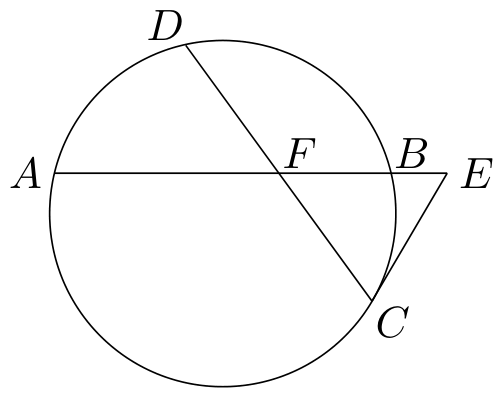
\includegraphics[width=6.0cm]{GaoKao/images/2011/tianjin_liberal/q13_fig1.png}
\end{center}

        \item 已知直角梯形 \(ABCD\) 中，\(AD \parallel BC\)，\(\angle ADC = 90^{\circ}\)，\(AD = 2\)，\(BC = 1\)，\(P\) 是腰 \(DC\) 上的动点，则 \(\left|\overrightarrow{PA}+3\overrightarrow{PB}\right|\) 的最小值为\rule[-0.3ex]{3em}{0.4pt}.

    \end{enumerate}

\end{description}

\begin{description}

    \item[三、解答题]

    \begin{enumerate}[leftmargin=5pt]

      \addtocounter{enumi}{+14}

        \item 编号分别为 \(A_{1}\)，\(A_{2}\)，\(\cdots\)，\(A_{16}\) 名篮球运动员在某次训练比赛中的得分记录如下：

\begin{center}
\begin{tabular}{|c|c|c|c|c|c|c|c|c|}
\hline
运动员编号 & \(A_{1}\) & \(A_{2}\) & \(A_{3}\) & \(A_{4}\) & \(A_{5}\) & \(A_{6}\) & \(A_{7}\) & \(A_{8}\) \\
\hline
得分 & 15 & 35 & 21 & 28 & 25 & 36 & 18 & 34 \\
\hline
运动员编号 & \(A_{9}\) & \(A_{10}\) & \(A_{11}\) & \(A_{12}\) & \(A_{13}\) & \(A_{14}\) & \(A_{15}\) & \(A_{16}\) \\
\hline
得分 & 17 & 26 & 25 & 33 & 22 & 12 & 31 & 38 \\
\hline
\end{tabular}
\end{center}

\begin{enumerate}
    \item 将得分在对应区间内的人数填入相应的空格；
    \begin{center}
    \begin{tabular}{|c|c|c|c|}
    \hline
    区间 & \([10,20)\) & \([20,30)\) & \([30,40]\) \\
    \hline
    人数 &\rule[-0.3ex]{3em}{0.4pt}&\rule[-0.3ex]{3em}{0.4pt}&\rule[-0.3ex]{3em}{0.4pt} \\
    \hline
    \end{tabular}
    \end{center}
    \item 从得分在区间 \([20, 30)\) 内的运动员中随机抽取 2 人，
    \begin{enumerate}
    \item 用运动员编号列出所有可能的抽取结果；
    \item 求这 2 人得分之和大于 50 的概率.
    \end{enumerate}
\end{enumerate}

        \item 在 \(\triangle ABC\) 中，内角 \(A\)，\(B\)，\(C\) 的对边分别为 \(a\)，\(b\)，\(c\)，已知 \(B = C\)，\(2b = \sqrt{3}a\).
\begin{enumerate}
\item 求 \(\cos A\) 的值；
\item \(\cos \left(2A + \frac{\pi}{4}\right)\) 的值.
\end{enumerate}

        \item 如图，在四棱锥 \(P - ABCD\) 中，底面 \(ABCD\) 为平行四边形，\(\angle ADC = 45^{\circ}\)，\(AD = AC = 1\)，\(O\) 为 \(AC\) 中点，\(PO \perp\) 平面 \(ABCD\)，\(PO = 2\)，\(M\) 为 \(PD\) 中点.
\begin{enumerate}
\item 证明： \(PB \parallel\) 平面 \(ACM\)；
\item 证明： \(AD \perp\) 平面 \(PAC\)；
\item 求直线 \(AM\) 与平面 \(ABCD\) 所成角的正切值.
\end{enumerate}

\begin{center}
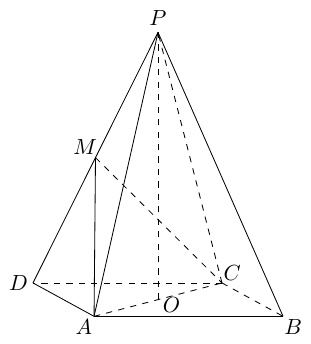
\includegraphics[width=7.7cm]{GaoKao/images/2011/tianjin_liberal/q17_fig1.png}
\end{center}

        \item 设椭圆 \(\frac{x^2}{a^{2}} + \frac{y^2}{b^{2}} = 1 \) （\(a > b > 0\)）的左、右焦点分别为 \(F_1\)，\(F_2\). 点 \(P(a, b)\) 满足 \(|PF_2| = |F_1F_2|\).
\begin{enumerate}
\item 求椭圆的离心率 \( e \)；
\item 设直线 \(PF_{2}\) 与椭圆相交于 \(A\)，\(B\) 两点，若直线 \(PF_{2}\) 与圆 \((x + 1)^{2} + (y - \sqrt{3})^{2} = 16\) 相交于 \(M\)，\(N\) 两点，且 \(|MN| = \frac{5}{8} |AB|\)，求椭圆的方程.
\end{enumerate}

        \item 已知函数 \(f(x) = 4x^{3} + 3tx^{2} - 6t^{2}x + t - 1\)，\(x \in \mathbb{R}\)，其中 \( t \in \mathbb{R}\).
\begin{enumerate}
\item 当 \(t = 1\) 时，求曲线 \(y = f(x)\) 在点 \((0, f(0))\) 处的切线方程；
\item 当 \(t \neq 0\) 时，求 \(f(x)\) 的单调区间；
\item 证明：对任意的 \(t \in (0, +\infty)\)，\(f(x)\) 在区间 \((0, 1)\) 内均存在零点.
\end{enumerate}

        \item 已知数列 \(\{a_{n}\}\) 与 \(\{b_{n}\}\) 满足： \(b_{n+1}a_{n} + b_{n}a_{n+1} = (-2)^{n} + 1\)，\(b_{n} = \frac{3 + (-1)^{n-1}}{2}\)，\(n \in \mathbb{N}^{*}\)，且 \(a_{1} = 2\).
\begin{enumerate}
\item 求 \(a_{2}\)，\(a_{3}\) 的值；
\item 设 \(c_{n} = a_{2n + 1} - a_{2n - 1}\)，\(n \in \mathbb{N}^{*}\)，证明：数列 \(\{c_{n}\}\) 是等比数列；
\item 设 \(S_{n}\) 为 \(\{a_{n}\}\) 的前 \(n\) 项和，证明 \(\frac{S_{1}}{a_{1}} + \frac{S_{2}}{a_{2}} + \ldots + \frac{S_{2n-1}}{a_{2n-1}} + \frac{S_{2n}}{a_{2n}} \leqslant n - \frac{1}{3}\) （\(n \in \mathbb{N}^{*}\)）.
\end{enumerate}

    \end{enumerate}

\end{description}


\subsection{2011年浙江卷（理）}\label{gk:2011年浙江卷（理）}

\begin{description}

    \item[一、选择题]

    \begin{enumerate}[leftmargin=5pt]

        \item 设函数 \( f(x) = \begin{cases}
-x, & x \leqslant 0,\\
x^2, & x > 0
\end{cases} \) 若 \( f(\alpha) = 4 \)，则实数 \( \alpha = \)（\quad）

        {\centering\begin{tabular*}{\linewidth}{@{}@{\extracolsep{\fill}}llll@{}}
          \text{A. }\(-4\) 或 \(-2\)  &  \text{B. }\(-4\) 或 2  &  \text{C. }\(-2\) 或 4  &  \text{D. }\(-2\) 或 2
        \end{tabular*}\par}

        \item 把复数 \(z\) 的共轭复数记作 \(\overline{z}\)，\(i\) 为虚数单位，若 \(z = 1 + \i\)，则 \((1 + z)\cdot \overline{z} =\)（\quad）

        {\centering\begin{tabular*}{\linewidth}{@{}@{\extracolsep{\fill}}llll@{}}
          \text{A. }\(3 - \i\)  &  \text{B. }\( 3 + \i \)  &  \text{C. }\( 1 + 3\i \)  &  \text{D. }\(3\)
        \end{tabular*}\par}

        \item 若某几何体的三视图如图所示，则这个几何体的直观图可以是（\quad）

\begin{center}
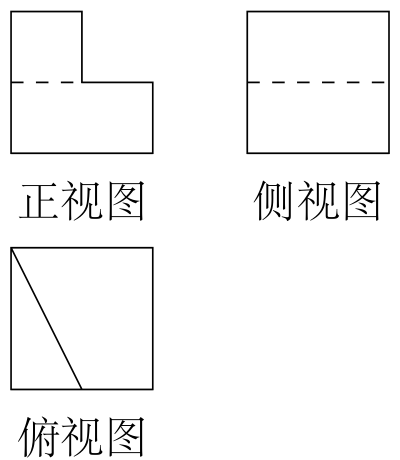
\includegraphics[width=3.9cm]{GaoKao/images/2011/zhejiang_science/q3_fig1.png}
\end{center}

        {\centering\begin{tabular*}{\linewidth}{@{}@{\extracolsep{\fill}}cccc@{}}
          \text{A. }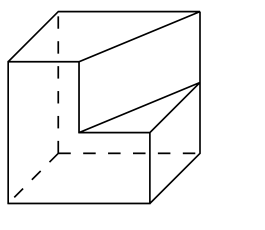
\includegraphics[width=0.15\paperwidth]{GaoKao/images/2011/zhejiang_science/q3_optA.png}  &  \text{B. }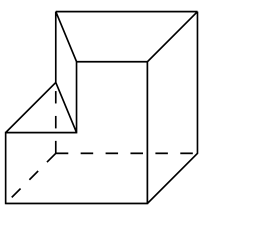
\includegraphics[width=0.15\paperwidth]{GaoKao/images/2011/zhejiang_science/q3_optB.png}  &  \text{C. }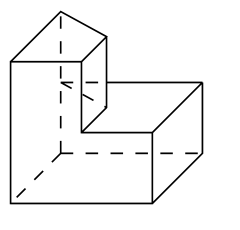
\includegraphics[width=0.15\paperwidth]{GaoKao/images/2011/zhejiang_science/q3_optC.png}  &  \text{D. }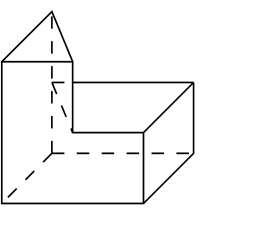
\includegraphics[width=0.15\paperwidth]{GaoKao/images/2011/zhejiang_science/q3_optD.png}
        \end{tabular*}\par}

        \item 下列命题中错误的是（\quad）

        {\centering\begin{tabular*}{\linewidth}{@{}@{\extracolsep{\fill}}llll@{}}
          \text{A. }如果平面 \(\alpha \perp\) 平面 \(\beta\)，那么平面 \(\alpha\) 内一定存在直线平行于平面 \(\beta\)  &  \text{B. }如果平面 \( \alpha \) 不垂直于平面 \( \beta \)，那么平面 \( \alpha \) 内一定不存在直线垂直于平面 \( \beta \)  &  \text{C. }如果平面 \(\alpha \perp\) 平面 \(\gamma\)，平面 \(\beta \perp\) 平面 \(\gamma\)，\(\alpha \cap \beta = l\)，那么 \(l \perp\) 平面 \(\gamma\)  &  \text{D. }如果平面 \(\alpha \perp\) 平面 \(\beta\)，那么平面 \(\alpha\) 内所有直线都垂直于平面 \(\beta\)
        \end{tabular*}\par}

        \item 设实数 \(x\)，\(y\) 满足不等式组 \(\begin{cases}
x + 2y - 5 > 0,\\
2x + y - 7 > 0,\\
x \geqslant 0, y \geqslant 0.
\end{cases}\) 若 \(x\)，\(y\) 为整数，则 \(3x + 4y\) 的最小值是（\quad）

        {\centering\begin{tabular*}{\linewidth}{@{}@{\extracolsep{\fill}}llll@{}}
          \text{A. }14  &  \text{B. }16  &  \text{C. }17  &  \text{D. }19
        \end{tabular*}\par}

        \item 若 \(0 < \alpha < \frac{\pi}{2}\)，\(-\frac{\pi}{2} < \beta < 0\)，\(\cos \left(\frac{\pi}{4} + \alpha\right) = \frac{1}{3}\)，\(\cos \left(\frac{\pi}{4} - \frac{\beta}{2}\right) = \frac{\sqrt{3}}{3}\)，则 \(\cos \left(\alpha + \frac{\beta}{2}\right) =\)（\quad）

        {\centering\begin{tabular*}{\linewidth}{@{}@{\extracolsep{\fill}}llll@{}}
          \text{A. }\(\frac{\sqrt{3}}{3}\)  &  \text{B. }\(-\frac{\sqrt{3}}{3}\)  &  \text{C. }\(\frac{5\sqrt{3}}{9}\)  &  \text{D. }\(-\frac{\sqrt{6}}{9}\)
        \end{tabular*}\par}

        \item 若 \(a\)，\(b\) 为实数，则 \(0 < ab < 1\) 是“\(a < \frac{1}{b}\) 或 \(b > \frac{1}{a}\)”的（\quad）

        {\centering\begin{tabular*}{\linewidth}{@{}@{\extracolsep{\fill}}llll@{}}
          \text{A. }充分而不必要条件  &  \text{B. }必要而不充分条件  &  \text{C. }充分必要条件  &  \text{D. }既不充分也不必要条件
        \end{tabular*}\par}

        \item 已知椭圆 \(C_{1}: \frac{x^{2}}{a^{2}} + \frac{y^{2}}{b^{2}} = 1\) （\(a > b > 0\)）与双曲线 \(C_2:  x^{2} - \frac{y^{2}}{4} = 1\) 有公共的焦点，\(C_2\) 的一条渐近线与以 \(C_1\) 的长轴为直径的圆相交于 \(A\)，\(B\) 两点. 若 \(C_1\) 恰好将线段 \(AB\) 三等分，则（\quad）

        {\centering\begin{tabular*}{\linewidth}{@{}@{\extracolsep{\fill}}llll@{}}
          \text{A. }\(a^2 = \frac{13}{2}\)  &  \text{B. }\(a^2 = 13\)  &  \text{C. }\(b^{2} = \frac{1}{2}\)  &  \text{D. }\(b^{2} = 2\)
        \end{tabular*}\par}

        \item 有 5 本不同的书，其中语文书 2 本，数学书 2 本，物理书 1 本. 若将其随机地抽取并摆放在书架的同一层上，则同一科目的书都不相邻的概率为（\quad）

        {\centering\begin{tabular*}{\linewidth}{@{}@{\extracolsep{\fill}}llll@{}}
          \text{A. }\(\frac{1}{5}\)  &  \text{B. }\(\frac{2}{5}\)  &  \text{C. }\(\frac{3}{5}\)  &  \text{D. }\(\frac{4}{5}\)
        \end{tabular*}\par}

        \item 设 \(a\)，\(b\)，\(c\) 为实数，\(f(x) = (x + a)(x^2 + bx + c)\)，\(g(x) = (ax + 1)(cx^2 + bx + 1)\). 记集合 \(S = \{x \mid f(x) = 0, x \in \mathbb{R}\}\)，\(T = \{x \mid g(x) = 0, x \in \mathbb{R}\}\)，若 \(|S|\)，\(|T|\) 分别为集合 \(S\)，\(T\) 的元素个数，则下列结论不可能的是（\quad）

        {\centering\begin{tabular*}{\linewidth}{@{}@{\extracolsep{\fill}}llll@{}}
          \text{A. }\( |S| = 1 \) 且 \( |T| = 0 \)  &  \text{B. }\( |S| = 1 \) 且 \( |T| = 1 \)  &  \text{C. }\( |S| = 2 \) 且 \( |T| = 2 \)  &  \text{D. }\( |S| = 2 \) 且 \( |T| = 3 \)
        \end{tabular*}\par}

    \end{enumerate}

\end{description}

\begin{description}

    \item[二、填空题]

    \begin{enumerate}[leftmargin=5pt]

      \addtocounter{enumi}{+10}

        \item 若函数 \( f(x) = x^2 - |x + a| \) 为偶函数，则实数 \( a = \)\rule[-0.3ex]{3em}{0.4pt}.

        \item 某程序框图如图所示，则该程序运行后输出的 \(k\) 的值是\rule[-0.3ex]{3em}{0.4pt}.

\begin{center}
\begin{center}
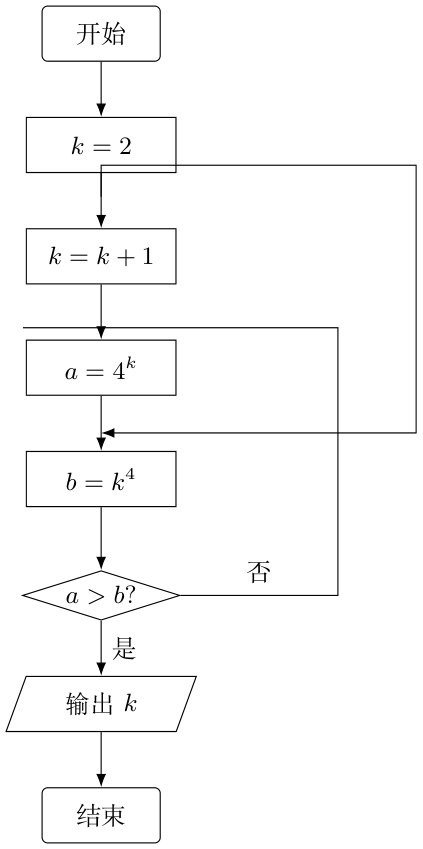
\includegraphics[width=0.70\linewidth]{GaoKao/images/2011/zhejiang_science/q12_fig1.png}
\end{center}
\end{center}

        \item 设二项式 \(\left(x - \frac{a}{\sqrt{x}}\right)^6\) （\(a > 0\)）的展开式中 \(x^3\) 的系数为 \(A\)，常数项为 \(B\). 若 \(B = 4A\)，则 \(a\) 的值是\rule[-0.3ex]{3em}{0.4pt}.

        \item 若平面向量 \(\alpha\)，\(\beta\) 满足 \(|\alpha| = 1\)，\(|\beta| \leqslant 1\)，且以向量 \(\alpha\)，\(\beta\) 为邻边的平行四边形的面积为 \(\frac{1}{2}\)，则 \(\alpha\) 和 \(\beta\) 的夹角 \(\theta\) 的取值范围是\rule[-0.3ex]{3em}{0.4pt}.

        \item 某毕业生参加人才招聘会，分别向甲，乙，丙三个公司投递了个人简历，假定该毕业生得到甲公司面试的概率为 \(\frac{2}{3}\)，得到乙，丙公司面试的概率均为 \(p\)，且三个公司是否让其面试是相互独立的. 记 \(X\) 为该毕业生得到面试的公司个数. 若 \(P(X = 0) = \frac{1}{12}\)，则随机变量 \(X\) 的数学期望 \(E(X) =\rule[-0.3ex]{3em}{0.4pt}\).

        \item 设 \(x\)，\(y\) 为实数. 若 \(4x^{2} + y^{2} + xy = 1\)，则 \(2x + y\) 的最大值是\rule[-0.3ex]{3em}{0.4pt}.

        \item 设 \(F_{1}\)，\(F_{2}\) 分别为椭圆 \(\frac{x^{2}}{3} + y^{2} = 1\) 的焦点，点 \(A\)，\(B\) 在椭圆上. 若 \(\overrightarrow{F_{1}A} = 5\overrightarrow{F_{2}B}\)，则点 \(A\) 的坐标是\rule[-0.3ex]{3em}{0.4pt}.

    \end{enumerate}

\end{description}

\begin{description}

    \item[三、解答题]

    \begin{enumerate}[leftmargin=5pt]

      \addtocounter{enumi}{+17}

        \item 在 \(\triangle ABC\) 中，角 \(A\)，\(B\)，\(C\) 所对的边分别为 \(a\)，\(b\)，\(c\). 已知 \(\sin A + \sin C = p \sin B\) （\(p \in \mathbb{R}\)），且 \(ac = \frac{1}{4} b^2\).
\begin{enumerate}
\item 当 \(p = \frac{5}{4}\)，\(b = 1\) 时，求 \(a\)，\(c\) 的值；
\item 若角 \(B\) 为锐角，求 \(p\) 的取值范围.
\end{enumerate}

        \item 已知公差不为 \(0\) 的等差数列 \(\{a_{n}\}\) 的首项 \(a_{1}\) 为 \(a\) （\(a\in\mathbb{R}\)）. 设数列的前 \(n\) 项和为 \(S_{n}\)，且 \(\frac{1}{a_{1}}\)，\(\frac{1}{a_{2}}\)，\(\frac{1}{a_{4}}\) 成等比数列.
\begin{enumerate}
\item 求数列 \( \{a_{n}\} \) 的通项公式及 \( S_{n} \)；
\item 记 \(A_{n} = \frac{1}{S_{1}} + \frac{1}{S_{2}} + \frac{1}{S_{3}} + \cdots + \frac{1}{S_{n}}\)，\(B_{n} = \frac{1}{a_{1}} + \frac{1}{a_{2}} + \frac{1}{a_{2^{2}}} + \cdots + \frac{1}{a_{2^{n-1}}}\) 当 \(n \geqslant 2\) 时，试比较 \(A_{n}\) 与 \(B_{n}\) 的大小.
\end{enumerate}

        \item 如图，在三棱锥 \(P - ABC\) 中，\(AB = AC\)，\(D\) 为 \(BC\) 的中点，\(PO \perp\) 平面 \(ABC\)，垂足 \(O\) 落在线段 \(AD\) 上，已知 \(BC = 8\)，\(PO = 4\)，\(AO = 3\)，\(OD = 2\).
\begin{enumerate}
\item 证明： \(AP \perp BC\)；
\item 在线段 \(AP\) 上是否存在点 \(M\)，使得二面角 \(A - MC - B\) 为直二面角. 若存在，求出 \(AM\) 的长；若不存在，请说明理由.
\end{enumerate}

\begin{center}
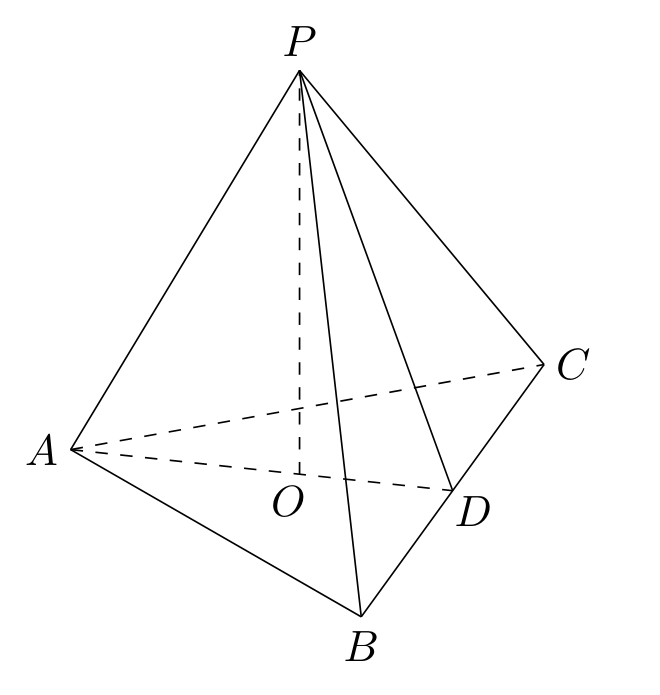
\includegraphics[width=7.0cm]{GaoKao/images/2011/zhejiang_science/q20_fig1.png}
\end{center}

        \item 已知抛物线 \(C_1: x^2 = y\)，圆 \(C_2: x^2 + (y - 4)^2 = 1\) 的圆心为点 \(M\).
\begin{enumerate}
\item 求点 \(M\) 到抛物线 \(C_{1}\) 的准线的距离；
\item 已知点 \(P\) 是抛物线 \(C_{1}\) 上一点 （异于原点），过点 \(P\) 作圆 \(C_{2}\) 的两条切线，交抛物线 \(C_{1}\) 于 \(A\)，\(B\) 两点，若过 \(M\)，\(P\) 两点的直线 \(l\) 垂直于 \(AB\)，求直线 \(l\) 的方程.
\end{enumerate}

\begin{center}
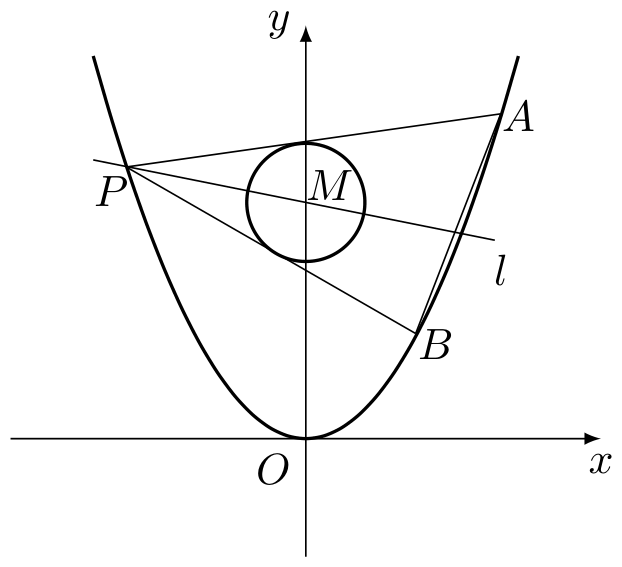
\includegraphics[width=7.2cm]{GaoKao/images/2011/zhejiang_science/q21_fig1.png}
\end{center}

        \item 设函数 \(f(x) = (x - a)^2 \ln x\)，\(a \in \mathbb{R}\).
\begin{enumerate}
\item 若 \(x = {\mathrm{e}}\) 为 \(y = f(x)\) 的极值点，求实数 \(a\)；
\item 求实数 \(a\) 的取值范围，使得对任意的 \(x \in (0,3{\mathrm{e}}]\)，恒有 \(f(x) \leqslant 4{\mathrm{e}}^2\) 成立. 注：\({\mathrm{e}}\) 为自然对数的底数.
\end{enumerate}

    \end{enumerate}

\end{description}


\subsection{2011年浙江卷（文）}\label{gk:2011年浙江卷（文）}

\begin{description}

    \item[一、选择题]

    \begin{enumerate}[leftmargin=5pt]

        \item 若 \(P = \{x \mid x < 1\}\)，\(Q = \{x \mid x > -1\}\)，则（\quad）

        {\centering\begin{tabular*}{\linewidth}{@{}@{\extracolsep{\fill}}llll@{}}
          \text{A. }\(P \subseteq Q\)  &  \text{B. }\(Q \subseteq P\)  &  \text{C. }\(\complement_{\mathbb{R}} P\subseteq Q\)  &  \text{D. }\(Q \subseteq \complement_{\mathbb{R}} P\)
        \end{tabular*}\par}

        \item 若复数 \(z = 1 + \i\)，\(\i\) 为虚数单位，则 \((1 + z)\cdot z =\)（\quad）

        {\centering\begin{tabular*}{\linewidth}{@{}@{\extracolsep{\fill}}llll@{}}
          \text{A. }\(1 + 3\i\)  &  \text{B. }\(3 + 3\i\)  &  \text{C. }\(3 - \i\)  &  \text{D. }\(3\)
        \end{tabular*}\par}

        \item 若实数 \(x\)，\(y\) 满足不等式组 \(\begin{cases}
x + 2y - 5 \geqslant 0,\\
2x + y - 7 \geqslant 0,\\
x \geqslant 0,\\
y \geqslant 0,
\end{cases}\) 则 \(3x + 4y\) 的最小值是（\quad）

        {\centering\begin{tabular*}{\linewidth}{@{}@{\extracolsep{\fill}}llll@{}}
          \text{A. }\(13\)  &  \text{B. }\(15\)  &  \text{C. }\(20\)  &  \text{D. }\(28\)
        \end{tabular*}\par}

        \item 若直线 \(l\) 不平行于平面 \(\alpha\)，且 \(l \not\subset \alpha\)，则（\quad）

        {\centering\begin{tabular*}{\linewidth}{@{}@{\extracolsep{\fill}}llll@{}}
          \text{A. }\(\alpha\) 内的所有直线与 \(l\) 异面  &  \text{B. }\(\alpha\) 内不存在与 \(l\) 平行的直线  &  \text{C. }\(\alpha\) 内存在唯一的直线与 \(l\) 平行  &  \text{D. }\(\alpha\) 内的直线与 \(l\) 都相交
        \end{tabular*}\par}

        \item 在 \(\triangle ABC\) 中，角 \(A\)，\(B\)，\(C\) 所对的边分别为 \(a\)，\(b\)，\(c\). 若 \(a \cos A = b \sin B\)，则 \(\sin A \cos A + \cos^2 B =\)（\quad）

        {\centering\begin{tabular*}{\linewidth}{@{}@{\extracolsep{\fill}}llll@{}}
          \text{A. }\(-\frac{1}{2}\)  &  \text{B. }\(\frac{1}{2}\)  &  \text{C. }\(-1\)  &  \text{D. }\(1\)
        \end{tabular*}\par}

        \item 若 \(a\)，\(b\) 为实数，则“\(0 < ab < 1\)”是“\(b < \frac{1}{a}\)”的（\quad）

        {\centering\begin{tabular*}{\linewidth}{@{}@{\extracolsep{\fill}}llll@{}}
          \text{A. }充分而不必要条件  &  \text{B. }必要而不充分条件  &  \text{C. }充分必要条件  &  \text{D. }既不充分也不必要条件
        \end{tabular*}\par}

        \item 若某几何体的三视图如图所示，则这个几何体的直观图可以是（\quad）

\begin{center}
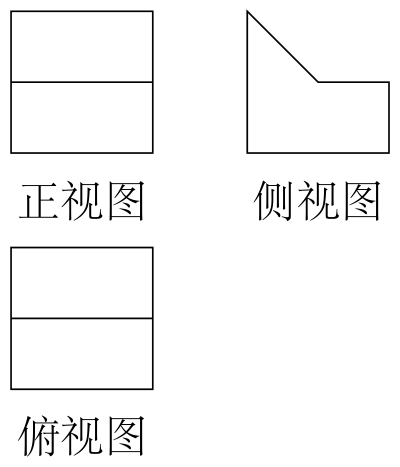
\includegraphics[width=3.9cm]{GaoKao/images/2011/zhejiang_liberal/q7_fig1.png}
\end{center}

        {\centering\begin{tabular*}{\linewidth}{@{}@{\extracolsep{\fill}}cccc@{}}
          \text{A. }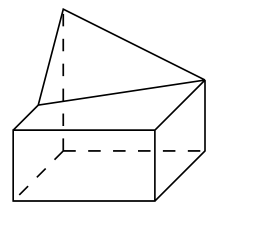
\includegraphics[width=0.15\paperwidth]{GaoKao/images/2011/zhejiang_liberal/q7_optA.png}  &  \text{B. }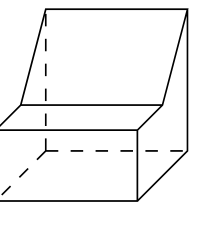
\includegraphics[width=0.15\paperwidth]{GaoKao/images/2011/zhejiang_liberal/q7_optB.png}  &  \text{C. }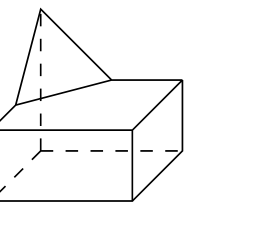
\includegraphics[width=0.15\paperwidth]{GaoKao/images/2011/zhejiang_liberal/q7_optC.png}  &  \text{D. }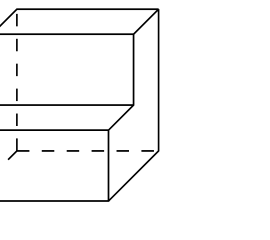
\includegraphics[width=0.15\paperwidth]{GaoKao/images/2011/zhejiang_liberal/q7_optD.png}
        \end{tabular*}\par}

        \item 从装有 3 个红球，2 个白球的袋中任取 3 个球，则所取的 3 个球中至少有 1 个白球的概率是（\quad）

        {\centering\begin{tabular*}{\linewidth}{@{}@{\extracolsep{\fill}}llll@{}}
          \text{A. }\( \frac{1}{10} \)  &  \text{B. }\( \frac{3}{10} \)  &  \text{C. }\( \frac{3}{5} \)  &  \text{D. }\( \frac{9}{10} \)
        \end{tabular*}\par}

        \item 已知椭圆 \(C_{1}: \frac{x^{2}}{a^{2}} + \frac{y^{2}}{b^{2}} = 1\) （\(a>b>0\)） 与双曲线 \(C_2: x^{2} - \frac{y^{2}}{4} = 1\) 有公共的焦点， \(C_2\) 的一条渐近线与以 \(C_1\) 的长轴为直径的圆相交于 \(A\)，\(B\) 两点. 若 \(C_1\) 恰好将线段 \(AB\) 三等分，则（\quad）

        {\centering\begin{tabular*}{\linewidth}{@{}@{\extracolsep{\fill}}llll@{}}
          \text{A. }\(a^2 = \frac{13}{2}\)  &  \text{B. }\(a^2 = 13\)  &  \text{C. }\(b^{2} = \frac{1}{2}\)  &  \text{D. }\(b^{2} = 2\)
        \end{tabular*}\par}

        \item 设函数 \( f(x) = ax^2 + bx + c \)，（\(a\)，\(b\)，\(c\in\mathbb{R}\)）. 若 \(x = -1\) 为函数 \( y = f(x){\mathrm{e}}^x \) 的一个极值点，则下列图象不可能为 \( y = f(x) \) 图象的是（\quad）

        {\centering\begin{tabular*}{\linewidth}{@{}@{\extracolsep{\fill}}cccc@{}}
          \text{A. }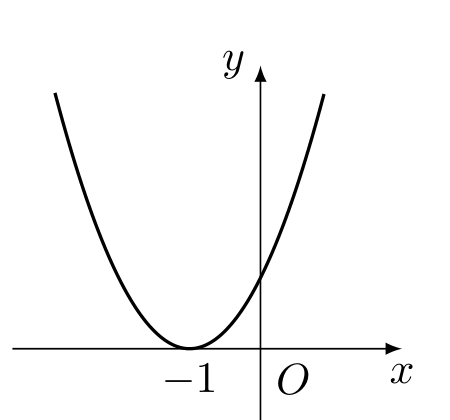
\includegraphics[width=0.15\paperwidth]{GaoKao/images/2011/zhejiang_liberal/q10_optA.png}  &  \text{B. }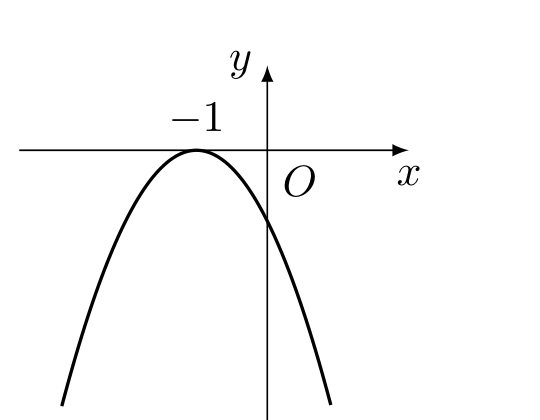
\includegraphics[width=0.15\paperwidth]{GaoKao/images/2011/zhejiang_liberal/q10_optB.png}  &  \text{C. }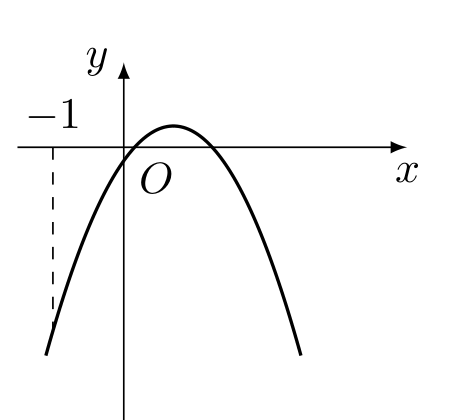
\includegraphics[width=0.15\paperwidth]{GaoKao/images/2011/zhejiang_liberal/q10_optC.png}  &  \text{D. }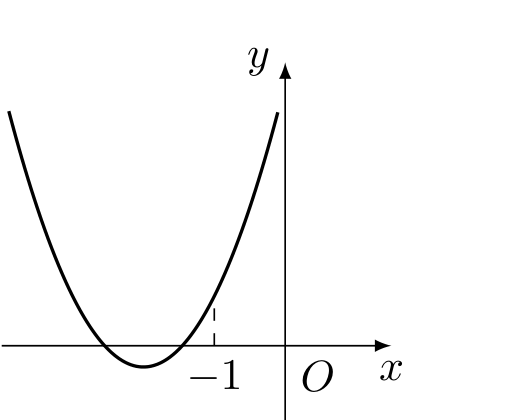
\includegraphics[width=0.15\paperwidth]{GaoKao/images/2011/zhejiang_liberal/q10_optD.png}
        \end{tabular*}\par}

    \end{enumerate}

\end{description}

\begin{description}

    \item[二、填空题]

    \begin{enumerate}[leftmargin=5pt]

      \addtocounter{enumi}{+10}

        \item 设函数 \( f(x) = \frac{4}{1 - x} \). 若 \( f(a) = 2 \)，则实数 \( a = \)\rule[-0.3ex]{3em}{0.4pt}.

        \item 若直线 \(x - 2y + 5 = 0\) 与直线 \(2x + my - 6 = 0\) 互相垂直，则实数 \(m = \)\rule[-0.3ex]{3em}{0.4pt}.

        \item 某小学为了解学生数学课程的学习情况，在 \(3000\) 名学生中随机抽取 \(200\) 名，并统计这 \(200\) 名学生的某次数学考试成绩，得到了样本的频率分布直方图（如图）. 根据频率分布直方图，\(3000\) 名学生在该次数学考试中成绩小于 \(60\) 分的学生数是\rule[-0.3ex]{3em}{0.4pt}.
\begin{center}
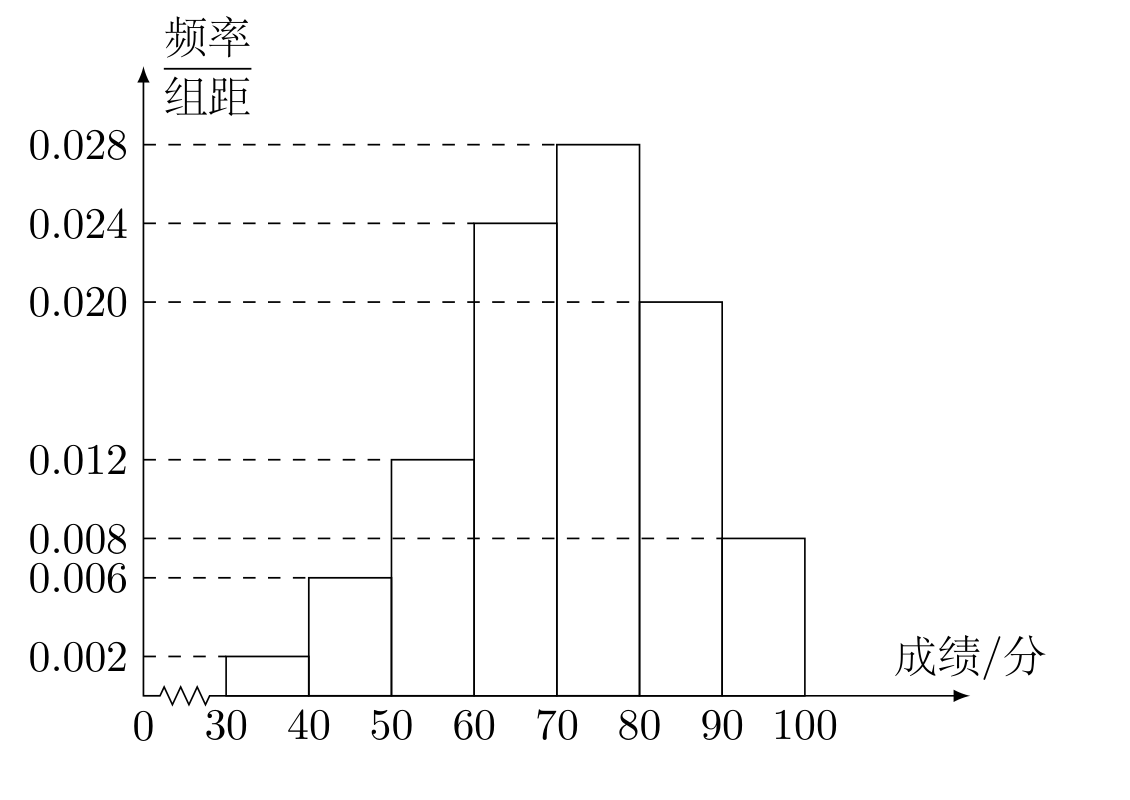
\includegraphics[width=0.42\linewidth]{GaoKao/images/2011/zhejiang_liberal/q13_fig1.png}
\end{center}

        \item 某程序框图如图所示，则该程序运行后输出的 \(k\) 的值是\rule[-0.3ex]{3em}{0.4pt}.
\begin{center}
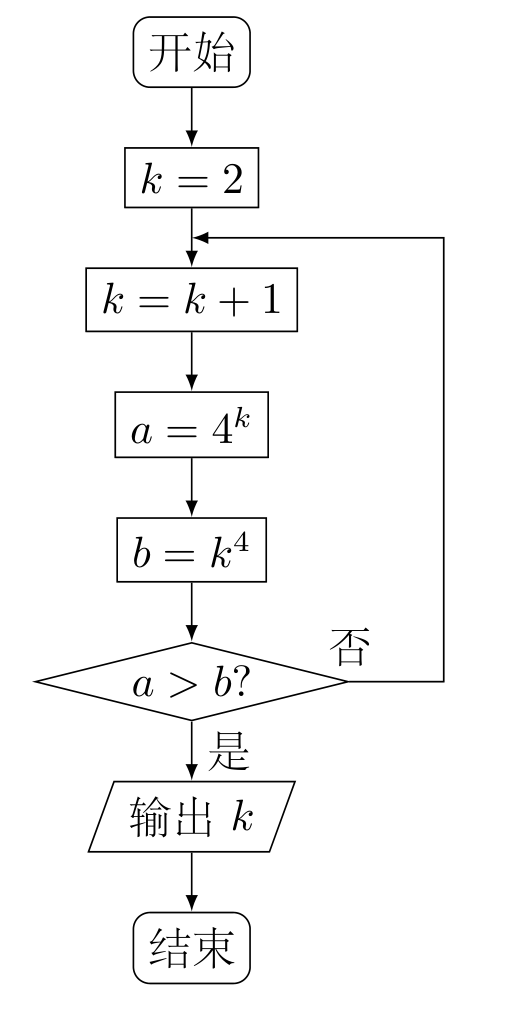
\includegraphics[width=0.70\linewidth]{GaoKao/images/2011/zhejiang_liberal/q14_fig1.png}
\end{center}

        \item 若平面向量 \(\bm{\alpha}\)，\(\bm{\beta}\) 满足 \(|\bm{\alpha}| = 1\)，\(|\bm{\beta}| \leqslant 1\)，且以向量 \(\bm{\alpha}\)，\(\bm{\beta}\) 为邻边的平行四边形的面积为 \(\frac{1}{2}\)，则 \(\bm{\alpha}\) 和 \(\bm{\beta}\) 的夹角 \(\theta\) 的取值范围是\rule[-0.3ex]{3em}{0.4pt}.

        \item 若实数 \(x\)，\(y\) 满足 \(x^{2} + y^{2} + xy = 1\)，则 \(x + y\) 的最大值是\rule[-0.3ex]{3em}{0.4pt}.

        \item 若数列 \(\left\{n(n + 4)\left(\frac{2}{3}\right)^n\right\}\) 中的最大项是第 \(k\) 项，则 \(k = \)\rule[-0.3ex]{3em}{0.4pt}.

    \end{enumerate}

\end{description}

\begin{description}

    \item[三、解答题]

    \begin{enumerate}[leftmargin=5pt]

      \addtocounter{enumi}{+17}

        \item 已知函数 \( f(x) = A \sin \left( \frac{\pi}{3} x + \varphi \right) \)，\( x \in \mathbb{R} \)，\(A > 0\)，\(0 < \varphi < \frac{\pi}{2}\). \( y = f(x) \) 的部分图象如图所示，\(P\)，\(Q\) 分别为该图象的最高点和最低点，点 \(P\) 的坐标为 \((1,A)\).

\begin{enumerate}
\item 求 \( f(x) \) 的最小正周期及 \( \varphi \) 的值；
\item 若点 \(R\) 的坐标为 \((1,0)\)，\(\angle PRQ = \frac{2\pi}{3}\)，求 \(A\) 的值.
\end{enumerate}

\begin{center}
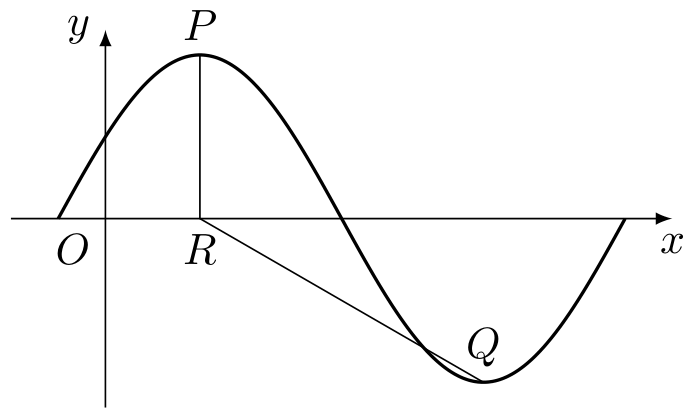
\includegraphics[width=4.0cm]{GaoKao/images/2011/zhejiang_liberal/q18_fig1.png}
\end{center}

        \item 已知公差不为 0 的等差数列 \(\{a_{n}\}\) 的首项 \(a_{1}\) 为 \(a\) （\(a \in \mathbb{R}\)），且 \(\frac{1}{a_1}\)，\(\frac{1}{a_2}\)，\(\frac{1}{a_4}\) 成等比数列.
\begin{enumerate}
\item 求数列 \( \{a_{n}\} \) 的通项公式；
\item 对 \(n \in \mathbb{N}^*\)，试比较 \(\frac{1}{a_2} + \frac{1}{a_{2^2}} + \frac{1}{a_{2^3}} + \cdots + \frac{1}{a_{2^n}}\) 与 \(\frac{1}{a_1}\) 的大小.
\end{enumerate}

        \item 如图，在三棱锥 \(P - ABC\) 中，\(AB = AC\)，\(D\) 为 \(BC\) 的中点，\(PO \perp\) 平面 \(ABC\)，垂足 \(O\) 落在线段 \(AD\) 上.
\begin{enumerate}
\item 证明： \(AP \perp BC\)；
\item 已知 \(BC = 8\)，\(PO = 4\)，\(AO = 3\)，\(OD = 2\). 求二面角 \(B - AP - C\) 的大小.
\end{enumerate}
\begin{center}
\includegraphics[width=7.7cm]{GaoKao/images/2011/zhejiang_liberal/q20_fig1.png}
\end{center}

        \item 设函数 \(f(x) = a^2 \ln x - x^2 + ax\)，\(a > 0\).
\begin{enumerate}
\item 求 \( f(x) \) 的单调区间；
\item 求所有实数 \(a\)，使 \({\mathrm{e}} - 1 \leqslant f(x) \leqslant {\mathrm{e}}^{2}\) 对 \(x \in [1, {\mathrm{e}}]\) 恒成立. 注：\({\mathrm{e}}\) 为自然对数的底数.
\end{enumerate}

        \item 如图，设 \(P\) 为抛物线 \(C_1: x^2 = y\) 上的动点，过点 \(P\) 做圆 \(C_2: x^2 + (y + 3)^2 = 1\) 的两条切线，交直线 \(l: y = -3\) 于 \(A\)，\(B\) 两点.
\begin{enumerate}
\item 求 \(C_{2}\) 的圆心 \(M\) 到抛物线 \(C_{1}\) 准线的距离.
\item 是否存在点 \(P\)，使线段 \(AB\) 被抛物线 \(C_1\) 在点 \(P\) 处的切线平分，若存在，求出点 \(P\) 的坐标；若不存在，请说明理由.
\end{enumerate}
\begin{center}
\includegraphics[width=5.5cm]{GaoKao/images/2011/zhejiang_liberal/q22_fig1.png}
\end{center}

    \end{enumerate}

\end{description}
